%% =====================================================================
%%  Electromagnetismo I · Tema 6 · Teoría del potencial (Parte I)
%%  Apuntes formalizados: Poisson y Laplace, identidades de Green,
%%  representación integral, unicidad y método de las imágenes.
%%  Compilar con:  pdflatex (dos pasadas)  ·  latexmk -pdf
%% =====================================================================
\documentclass[11pt,a4paper,twoside]{article}
\usepackage{estilo/tema6-estilo}

\hypersetup{pdftitle={Tema 6. Teoría del potencial (Parte I)},
            pdfauthor={Daniel Martín Guerrero},
            pdfsubject={Electromagnetismo I}}

\begin{document}

%% ------------------------------------------------------------- PORTADA
\begin{titlepage}
  \newgeometry{top=1.6cm,bottom=1.6cm,left=2.4cm,right=2.4cm}
  \centering
  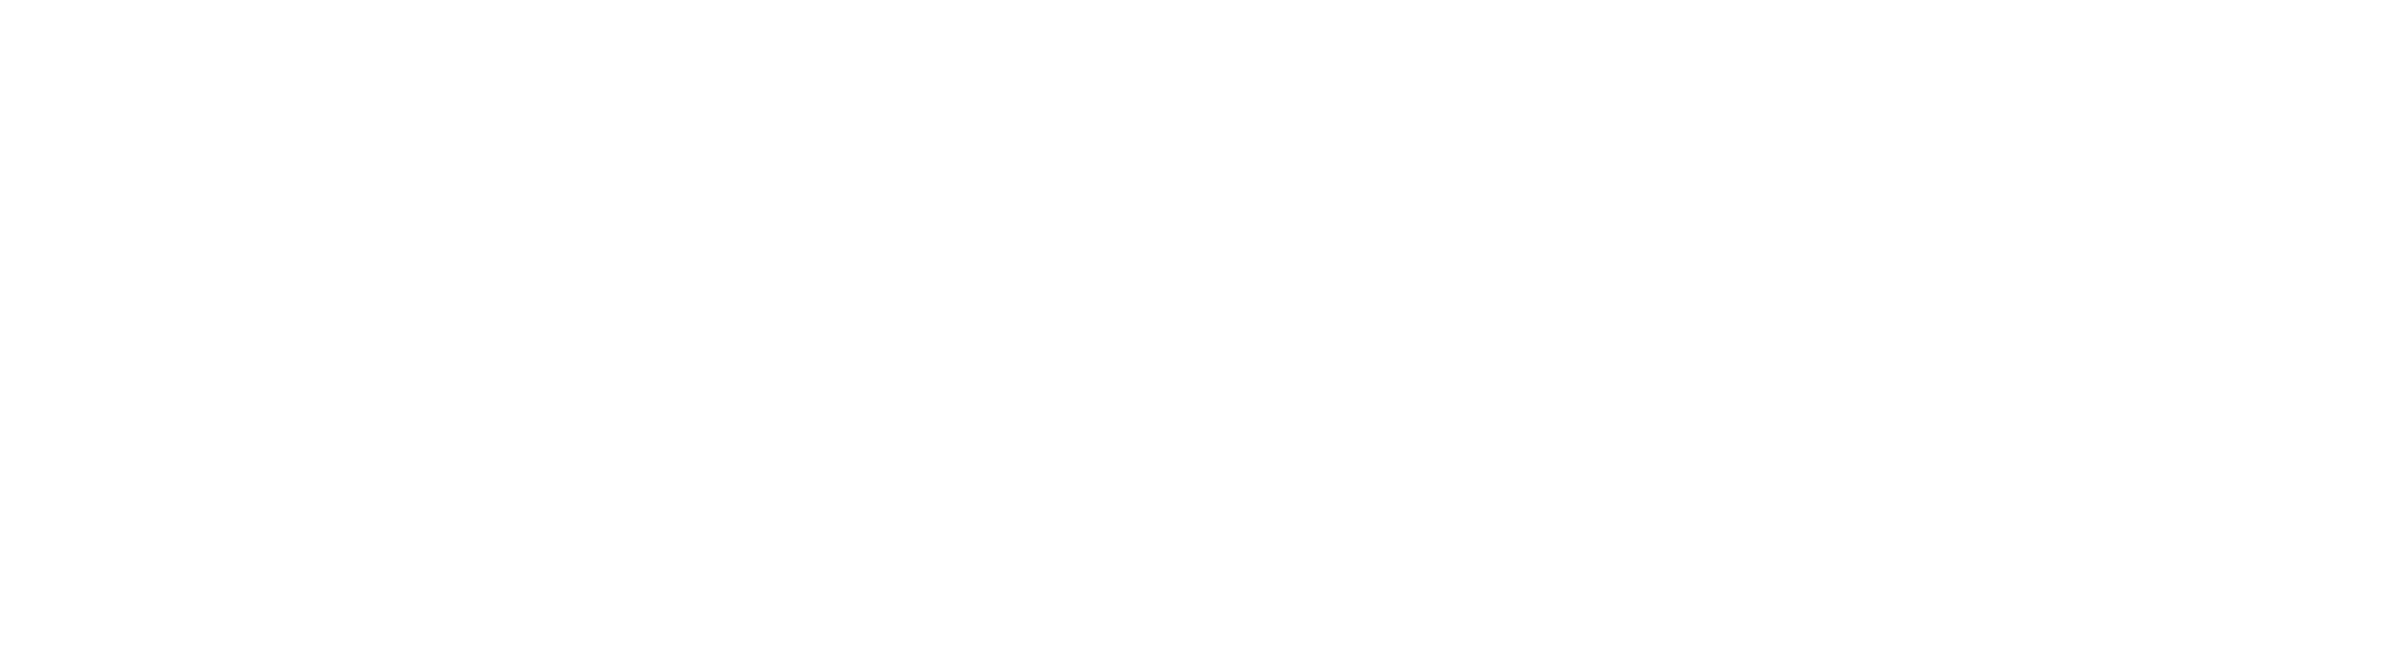
\includegraphics[width=4.4cm]{estilo/logo-usal.png}\par
  \vspace{0.55cm}
  {\color{gristexto}\rule{\textwidth}{0.4pt}}\par\vspace{0.35cm}
  {\color{gristexto}\textsc{Facultad de Ciencias \quad$\cdot$\quad Grado en Física}}\par
  \vspace{0.9cm}
  {\color{azul}\large\textsc{Electromagnetismo I}}\par\vspace{0.12cm}
  {\color{gristexto}\textsc{Tema 6 \textperiodcentered{} Parte I}}\par
  \vspace{0.7cm}
  {\fontsize{29}{34}\selectfont\bfseries\color{texto} Teoría del potencial}\par
  \vspace{0.45cm}
  {\color{gristexto}\rule{3.2cm}{0.4pt}}\par\vspace{0.4cm}
  {\color{gristexto}\itshape Ecuaciones de Poisson y Laplace \,$\cdot$\, Identidades de Green
   y representación integral\\ Unicidad de la solución \,$\cdot$\, Método de las imágenes}\par
  \vspace{0.7cm}
  % =====================================================================
% Figura de portada (minimalista): carga puntual frente a una esfera conductora a tierra.
% Líneas de campo exactas (método de las imágenes, a = 1, d = 2) con
% degradado azul -> oro según el ángulo de salida; equipotenciales
% punteadas. Datos: figuras/datos/portada.tex (generar_figuras.py).
% =====================================================================
\begin{tikzpicture}
  \def\esc{1.7}
  \begin{scope}
    \clip (-2.25*\esc,-2.3*\esc) rectangle (5.05*\esc,2.3*\esc);
    % Generado automáticamente por generar_figuras.py; no editar.
\draw[line width=0.55pt, color={rgb,255:red,60;green,110;blue,200}, opacity=0.9] plot coordinates {(3.318,0.023) (3.253,0.042) (3.187,0.061) (3.122,0.079) (3.057,0.097) (2.991,0.116) (2.925,0.134) (2.860,0.151) (2.794,0.169) (2.728,0.185) (2.662,0.202) (2.596,0.217) (2.530,0.232) (2.463,0.246) (2.396,0.259) (2.329,0.270) (2.262,0.280) (2.194,0.288) (2.127,0.294) (2.059,0.299) (1.991,0.301) (1.923,0.300) (1.855,0.297) (1.787,0.291) (1.720,0.283) (1.677,0.277)};
\draw[line width=0.55pt, color={rgb,255:red,60;green,110;blue,200}, opacity=0.9] plot coordinates {(3.318,-0.023) (3.253,-0.042) (3.187,-0.061) (3.122,-0.079) (3.057,-0.097) (2.991,-0.116) (2.925,-0.134) (2.860,-0.151) (2.794,-0.169) (2.728,-0.185) (2.662,-0.202) (2.596,-0.217) (2.530,-0.232) (2.463,-0.246) (2.396,-0.259) (2.329,-0.270) (2.262,-0.280) (2.194,-0.288) (2.127,-0.294) (2.059,-0.299) (1.991,-0.301) (1.923,-0.300) (1.855,-0.297) (1.787,-0.291) (1.720,-0.283) (1.677,-0.277)};
\draw[line width=0.55pt, color={rgb,255:red,64;green,119;blue,204}, opacity=0.9] plot coordinates {(3.325,0.040) (3.265,0.071) (3.204,0.103) (3.144,0.134) (3.084,0.166) (3.023,0.197) (2.963,0.227) (2.902,0.257) (2.840,0.287) (2.779,0.316) (2.717,0.344) (2.655,0.372) (2.592,0.398) (2.529,0.423) (2.465,0.446) (2.400,0.467) (2.335,0.487) (2.269,0.504) (2.203,0.518) (2.136,0.530) (2.068,0.538) (2.001,0.543) (1.933,0.544) (1.865,0.540) (1.797,0.533) (1.730,0.522) (1.664,0.506) (1.626,0.496)};
\draw[line width=0.55pt, color={rgb,255:red,64;green,119;blue,204}, opacity=0.9] plot coordinates {(3.325,-0.040) (3.265,-0.071) (3.204,-0.103) (3.144,-0.134) (3.084,-0.166) (3.023,-0.197) (2.963,-0.227) (2.902,-0.257) (2.840,-0.287) (2.779,-0.316) (2.717,-0.344) (2.655,-0.372) (2.592,-0.398) (2.529,-0.423) (2.465,-0.446) (2.400,-0.467) (2.335,-0.487) (2.269,-0.504) (2.203,-0.518) (2.136,-0.530) (2.068,-0.538) (2.001,-0.543) (1.933,-0.544) (1.865,-0.540) (1.797,-0.533) (1.730,-0.522) (1.664,-0.506) (1.626,-0.496)};
\draw[line width=0.55pt, color={rgb,255:red,69;green,128;blue,209}, opacity=0.9] plot coordinates {(3.331,0.050) (3.276,0.090) (3.221,0.130) (3.166,0.170) (3.111,0.209) (3.055,0.249) (3.000,0.288) (2.944,0.326) (2.887,0.364) (2.830,0.401) (2.773,0.438) (2.715,0.473) (2.656,0.507) (2.596,0.540) (2.536,0.571) (2.475,0.601) (2.413,0.628) (2.349,0.653) (2.285,0.676) (2.220,0.695) (2.154,0.711) (2.087,0.723) (2.019,0.731) (1.952,0.735) (1.884,0.734) (1.816,0.729) (1.749,0.718) (1.682,0.703) (1.618,0.682) (1.566,0.662)};
\draw[line width=0.55pt, color={rgb,255:red,69;green,128;blue,209}, opacity=0.9] plot coordinates {(3.331,-0.050) (3.276,-0.090) (3.221,-0.130) (3.166,-0.170) (3.111,-0.209) (3.055,-0.249) (3.000,-0.288) (2.944,-0.326) (2.887,-0.364) (2.830,-0.401) (2.773,-0.438) (2.715,-0.473) (2.656,-0.507) (2.596,-0.540) (2.536,-0.571) (2.475,-0.601) (2.413,-0.628) (2.349,-0.653) (2.285,-0.676) (2.220,-0.695) (2.154,-0.711) (2.087,-0.723) (2.019,-0.731) (1.952,-0.735) (1.884,-0.734) (1.816,-0.729) (1.749,-0.718) (1.682,-0.703) (1.618,-0.682) (1.566,-0.662)};
\draw[line width=0.55pt, color={rgb,255:red,74;green,138;blue,214}, opacity=0.9] plot coordinates {(3.338,0.058) (3.288,0.104) (3.238,0.151) (3.188,0.197) (3.138,0.243) (3.088,0.288) (3.037,0.334) (2.986,0.378) (2.934,0.423) (2.882,0.466) (2.829,0.509) (2.776,0.551) (2.721,0.592) (2.666,0.631) (2.609,0.669) (2.552,0.706) (2.493,0.740) (2.434,0.772) (2.372,0.802) (2.310,0.829) (2.246,0.853) (2.182,0.874) (2.116,0.891) (2.049,0.903) (1.982,0.912) (1.914,0.915) (1.846,0.913) (1.778,0.906) (1.711,0.894) (1.646,0.876) (1.582,0.854) (1.520,0.825) (1.494,0.812)};
\draw[line width=0.55pt, color={rgb,255:red,74;green,138;blue,214}, opacity=0.9] plot coordinates {(3.338,-0.058) (3.288,-0.104) (3.238,-0.151) (3.188,-0.197) (3.138,-0.243) (3.088,-0.288) (3.037,-0.334) (2.986,-0.378) (2.934,-0.423) (2.882,-0.466) (2.829,-0.509) (2.776,-0.551) (2.721,-0.592) (2.666,-0.631) (2.609,-0.669) (2.552,-0.706) (2.493,-0.740) (2.434,-0.772) (2.372,-0.802) (2.310,-0.829) (2.246,-0.853) (2.182,-0.874) (2.116,-0.891) (2.049,-0.903) (1.982,-0.912) (1.914,-0.915) (1.846,-0.913) (1.778,-0.906) (1.711,-0.894) (1.646,-0.876) (1.582,-0.854) (1.520,-0.825) (1.494,-0.812)};
\draw[line width=0.55pt, color={rgb,255:red,79;green,147;blue,219}, opacity=0.9] plot coordinates {(3.344,0.064) (3.300,0.116) (3.255,0.167) (3.210,0.218) (3.165,0.269) (3.120,0.320) (3.074,0.370) (3.028,0.420) (2.982,0.469) (2.934,0.518) (2.886,0.566) (2.837,0.614) (2.787,0.660) (2.737,0.705) (2.685,0.749) (2.631,0.791) (2.577,0.832) (2.521,0.871) (2.464,0.908) (2.405,0.942) (2.345,0.974) (2.284,1.003) (2.221,1.028) (2.156,1.050) (2.091,1.068) (2.024,1.082) (1.957,1.091) (1.889,1.095) (1.821,1.095) (1.753,1.088) (1.686,1.076) (1.621,1.059) (1.557,1.036) (1.495,1.007) (1.436,0.974) (1.407,0.955)};
\draw[line width=0.55pt, color={rgb,255:red,79;green,147;blue,219}, opacity=0.9] plot coordinates {(3.344,-0.064) (3.300,-0.116) (3.255,-0.167) (3.210,-0.218) (3.165,-0.269) (3.120,-0.320) (3.074,-0.370) (3.028,-0.420) (2.982,-0.469) (2.934,-0.518) (2.886,-0.566) (2.837,-0.614) (2.787,-0.660) (2.737,-0.705) (2.685,-0.749) (2.631,-0.791) (2.577,-0.832) (2.521,-0.871) (2.464,-0.908) (2.405,-0.942) (2.345,-0.974) (2.284,-1.003) (2.221,-1.028) (2.156,-1.050) (2.091,-1.068) (2.024,-1.082) (1.957,-1.091) (1.889,-1.095) (1.821,-1.095) (1.753,-1.088) (1.686,-1.076) (1.621,-1.059) (1.557,-1.036) (1.495,-1.007) (1.436,-0.974) (1.407,-0.955)};
\draw[line width=0.55pt, color={rgb,255:red,84;green,157;blue,224}, opacity=0.9] plot coordinates {(3.351,0.069) (3.312,0.125) (3.272,0.180) (3.233,0.236) (3.193,0.291) (3.153,0.346) (3.112,0.400) (3.071,0.454) (3.029,0.508) (2.987,0.561) (2.943,0.614) (2.899,0.665) (2.854,0.716) (2.808,0.766) (2.761,0.815) (2.713,0.863) (2.663,0.909) (2.612,0.954) (2.559,0.997) (2.505,1.038) (2.449,1.077) (2.391,1.113) (2.332,1.147) (2.272,1.178) (2.210,1.206) (2.146,1.230) (2.081,1.250) (2.015,1.266) (1.948,1.277) (1.881,1.284) (1.813,1.286) (1.745,1.282) (1.677,1.273) (1.611,1.258) (1.546,1.238) (1.483,1.212) (1.423,1.181) (1.365,1.145) (1.311,1.104) (1.300,1.095)};
\draw[line width=0.55pt, color={rgb,255:red,84;green,157;blue,224}, opacity=0.9] plot coordinates {(3.351,-0.069) (3.312,-0.125) (3.272,-0.180) (3.233,-0.236) (3.193,-0.291) (3.153,-0.346) (3.112,-0.400) (3.071,-0.454) (3.029,-0.508) (2.987,-0.561) (2.943,-0.614) (2.899,-0.665) (2.854,-0.716) (2.808,-0.766) (2.761,-0.815) (2.713,-0.863) (2.663,-0.909) (2.612,-0.954) (2.559,-0.997) (2.505,-1.038) (2.449,-1.077) (2.391,-1.113) (2.332,-1.147) (2.272,-1.178) (2.210,-1.206) (2.146,-1.230) (2.081,-1.250) (2.015,-1.266) (1.948,-1.277) (1.881,-1.284) (1.813,-1.286) (1.745,-1.282) (1.677,-1.273) (1.611,-1.258) (1.546,-1.238) (1.483,-1.212) (1.423,-1.181) (1.365,-1.145) (1.311,-1.104) (1.300,-1.095)};
\draw[line width=0.55pt, color={rgb,255:red,88;green,166;blue,228}, opacity=0.9] plot coordinates {(3.357,0.074) (3.323,0.132) (3.289,0.191) (3.255,0.250) (3.220,0.308) (3.185,0.367) (3.150,0.425) (3.113,0.482) (3.077,0.540) (3.039,0.596) (3.001,0.653) (2.962,0.708) (2.922,0.763) (2.881,0.817) (2.839,0.871) (2.795,0.923) (2.750,0.974) (2.704,1.024) (2.656,1.072) (2.607,1.119) (2.556,1.164) (2.504,1.208) (2.450,1.249) (2.394,1.287) (2.336,1.324) (2.277,1.357) (2.216,1.388) (2.154,1.415) (2.090,1.438) (2.025,1.458) (1.959,1.474) (1.892,1.485) (1.824,1.491) (1.756,1.493) (1.688,1.489) (1.621,1.480) (1.555,1.465) (1.490,1.445) (1.427,1.420) (1.366,1.389) (1.308,1.354) (1.253,1.313) (1.202,1.269) (1.168,1.235)};
\draw[line width=0.55pt, color={rgb,255:red,88;green,166;blue,228}, opacity=0.9] plot coordinates {(3.357,-0.074) (3.323,-0.132) (3.289,-0.191) (3.255,-0.250) (3.220,-0.308) (3.185,-0.367) (3.150,-0.425) (3.113,-0.482) (3.077,-0.540) (3.039,-0.596) (3.001,-0.653) (2.962,-0.708) (2.922,-0.763) (2.881,-0.817) (2.839,-0.871) (2.795,-0.923) (2.750,-0.974) (2.704,-1.024) (2.656,-1.072) (2.607,-1.119) (2.556,-1.164) (2.504,-1.208) (2.450,-1.249) (2.394,-1.287) (2.336,-1.324) (2.277,-1.357) (2.216,-1.388) (2.154,-1.415) (2.090,-1.438) (2.025,-1.458) (1.959,-1.474) (1.892,-1.485) (1.824,-1.491) (1.756,-1.493) (1.688,-1.489) (1.621,-1.480) (1.555,-1.465) (1.490,-1.445) (1.427,-1.420) (1.366,-1.389) (1.308,-1.354) (1.253,-1.313) (1.202,-1.269) (1.168,-1.235)};
\draw[line width=0.55pt, color={rgb,255:red,90;green,172;blue,225}, opacity=0.9] plot coordinates {(3.364,0.077) (3.335,0.139) (3.306,0.200) (3.277,0.262) (3.247,0.323) (3.218,0.384) (3.187,0.445) (3.156,0.505) (3.125,0.566) (3.093,0.625) (3.059,0.685) (3.026,0.744) (2.991,0.802) (2.955,0.860) (2.917,0.917) (2.879,0.973) (2.840,1.028) (2.799,1.082) (2.756,1.136) (2.712,1.187) (2.667,1.238) (2.620,1.287) (2.571,1.335) (2.521,1.380) (2.468,1.424) (2.415,1.466) (2.359,1.505) (2.302,1.542) (2.243,1.576) (2.183,1.607) (2.121,1.635) (2.058,1.660) (1.993,1.681) (1.927,1.699) (1.861,1.712) (1.793,1.721) (1.725,1.725) (1.657,1.724) (1.590,1.719) (1.523,1.708) (1.456,1.692) (1.392,1.671) (1.329,1.645) (1.269,1.614) (1.211,1.578) (1.157,1.537) (1.106,1.492) (1.059,1.443) (1.015,1.391) (1.002,1.373)};
\draw[line width=0.55pt, color={rgb,255:red,90;green,172;blue,225}, opacity=0.9] plot coordinates {(3.364,-0.077) (3.335,-0.139) (3.306,-0.200) (3.277,-0.262) (3.247,-0.323) (3.218,-0.384) (3.187,-0.445) (3.156,-0.505) (3.125,-0.566) (3.093,-0.625) (3.059,-0.685) (3.026,-0.744) (2.991,-0.802) (2.955,-0.860) (2.917,-0.917) (2.879,-0.973) (2.840,-1.028) (2.799,-1.082) (2.756,-1.136) (2.712,-1.187) (2.667,-1.238) (2.620,-1.287) (2.571,-1.335) (2.521,-1.380) (2.468,-1.424) (2.415,-1.466) (2.359,-1.505) (2.302,-1.542) (2.243,-1.576) (2.183,-1.607) (2.121,-1.635) (2.058,-1.660) (1.993,-1.681) (1.927,-1.699) (1.861,-1.712) (1.793,-1.721) (1.725,-1.725) (1.657,-1.724) (1.590,-1.719) (1.523,-1.708) (1.456,-1.692) (1.392,-1.671) (1.329,-1.645) (1.269,-1.614) (1.211,-1.578) (1.157,-1.537) (1.106,-1.492) (1.059,-1.443) (1.015,-1.391) (1.002,-1.373)};
\draw[line width=0.55pt, color={rgb,255:red,90;green,177;blue,218}, opacity=0.9] plot coordinates {(3.371,0.080) (3.347,0.144) (3.323,0.207) (3.299,0.271) (3.275,0.334) (3.250,0.398) (3.225,0.461) (3.199,0.524) (3.173,0.586) (3.146,0.649) (3.118,0.711) (3.089,0.773) (3.060,0.834) (3.029,0.894) (2.997,0.954) (2.964,1.014) (2.930,1.073) (2.894,1.131) (2.857,1.188) (2.819,1.244) (2.779,1.299) (2.738,1.353) (2.695,1.406) (2.651,1.457) (2.605,1.507) (2.557,1.556) (2.508,1.603) (2.457,1.648) (2.404,1.691) (2.350,1.732) (2.294,1.770) (2.236,1.807) (2.177,1.840) (2.117,1.871) (2.055,1.899) (1.991,1.924) (1.927,1.945) (1.861,1.963) (1.795,1.977) (1.727,1.987) (1.660,1.993) (1.592,1.995) (1.524,1.992) (1.456,1.984) (1.389,1.972) (1.324,1.955) (1.259,1.932) (1.197,1.905) (1.137,1.874) (1.079,1.838) (1.025,1.797) (0.974,1.752) (0.926,1.704) (0.882,1.652) (0.842,1.596) (0.807,1.539) (0.789,1.506)};
\draw[line width=0.55pt, color={rgb,255:red,90;green,177;blue,218}, opacity=0.9] plot coordinates {(3.371,-0.080) (3.347,-0.144) (3.323,-0.207) (3.299,-0.271) (3.275,-0.334) (3.250,-0.398) (3.225,-0.461) (3.199,-0.524) (3.173,-0.586) (3.146,-0.649) (3.118,-0.711) (3.089,-0.773) (3.060,-0.834) (3.029,-0.894) (2.997,-0.954) (2.964,-1.014) (2.930,-1.073) (2.894,-1.131) (2.857,-1.188) (2.819,-1.244) (2.779,-1.299) (2.738,-1.353) (2.695,-1.406) (2.651,-1.457) (2.605,-1.507) (2.557,-1.556) (2.508,-1.603) (2.457,-1.648) (2.404,-1.691) (2.350,-1.732) (2.294,-1.770) (2.236,-1.807) (2.177,-1.840) (2.117,-1.871) (2.055,-1.899) (1.991,-1.924) (1.927,-1.945) (1.861,-1.963) (1.795,-1.977) (1.727,-1.987) (1.660,-1.993) (1.592,-1.995) (1.524,-1.992) (1.456,-1.984) (1.389,-1.972) (1.324,-1.955) (1.259,-1.932) (1.197,-1.905) (1.137,-1.874) (1.079,-1.838) (1.025,-1.797) (0.974,-1.752) (0.926,-1.704) (0.882,-1.652) (0.842,-1.596) (0.807,-1.539) (0.789,-1.506)};
\draw[line width=0.55pt, color={rgb,255:red,90;green,182;blue,212}, opacity=0.9] plot coordinates {(3.377,0.082) (3.359,0.147) (3.340,0.213) (3.321,0.278) (3.302,0.343) (3.283,0.408) (3.263,0.474) (3.242,0.538) (3.221,0.603) (3.199,0.667) (3.177,0.731) (3.153,0.795) (3.129,0.859) (3.103,0.922) (3.077,0.985) (3.050,1.047) (3.021,1.108) (2.991,1.169) (2.960,1.230) (2.927,1.290) (2.893,1.349) (2.858,1.407) (2.821,1.464) (2.783,1.520) (2.744,1.575) (2.702,1.630) (2.660,1.682) (2.615,1.734) (2.569,1.784) (2.522,1.833) (2.473,1.880) (2.422,1.925) (2.370,1.969) (2.317,2.011) (2.261,2.050) (2.205,2.088) (2.146,2.123) (2.087,2.156) (2.026,2.186) (1.964,2.214) (1.900,2.238) (1.836,2.260) (1.771,2.279) (1.704,2.294) (1.637,2.305) (1.570,2.314) (1.502,2.318) (1.434,2.318) (1.366,2.314) (1.299,2.306) (1.232,2.294) (1.166,2.277) (1.101,2.256) (1.038,2.231) (0.977,2.201) (0.918,2.167) (0.862,2.129) (0.809,2.087) (0.759,2.041) (0.712,1.991) (0.669,1.938) (0.630,1.883) (0.595,1.825) (0.563,1.764) (0.536,1.702) (0.513,1.638) (0.508,1.622)};
\draw[line width=0.55pt, color={rgb,255:red,90;green,182;blue,212}, opacity=0.9] plot coordinates {(3.377,-0.082) (3.359,-0.147) (3.340,-0.213) (3.321,-0.278) (3.302,-0.343) (3.283,-0.408) (3.263,-0.474) (3.242,-0.538) (3.221,-0.603) (3.199,-0.667) (3.177,-0.731) (3.153,-0.795) (3.129,-0.859) (3.103,-0.922) (3.077,-0.985) (3.050,-1.047) (3.021,-1.108) (2.991,-1.169) (2.960,-1.230) (2.927,-1.290) (2.893,-1.349) (2.858,-1.407) (2.821,-1.464) (2.783,-1.520) (2.744,-1.575) (2.702,-1.630) (2.660,-1.682) (2.615,-1.734) (2.569,-1.784) (2.522,-1.833) (2.473,-1.880) (2.422,-1.925) (2.370,-1.969) (2.317,-2.011) (2.261,-2.050) (2.205,-2.088) (2.146,-2.123) (2.087,-2.156) (2.026,-2.186) (1.964,-2.214) (1.900,-2.238) (1.836,-2.260) (1.771,-2.279) (1.704,-2.294) (1.637,-2.305) (1.570,-2.314) (1.502,-2.318) (1.434,-2.318) (1.366,-2.314) (1.299,-2.306) (1.232,-2.294) (1.166,-2.277) (1.101,-2.256) (1.038,-2.231) (0.977,-2.201) (0.918,-2.167) (0.862,-2.129) (0.809,-2.087) (0.759,-2.041) (0.712,-1.991) (0.669,-1.938) (0.630,-1.883) (0.595,-1.825) (0.563,-1.764) (0.536,-1.702) (0.513,-1.638) (0.508,-1.622)};
\draw[line width=0.55pt, color={rgb,255:red,90;green,187;blue,206}, opacity=0.9] plot coordinates {(3.384,0.083) (3.370,0.150) (3.357,0.217) (3.344,0.283) (3.330,0.350) (3.315,0.416) (3.301,0.483) (3.285,0.549) (3.270,0.615) (3.253,0.681) (3.236,0.747) (3.218,0.813) (3.199,0.878) (3.179,0.943) (3.158,1.008) (3.136,1.072) (3.113,1.136) (3.089,1.199) (3.063,1.263) (3.037,1.325) (3.009,1.387) (2.980,1.449) (2.949,1.509) (2.918,1.570) (2.884,1.629) (2.850,1.688) (2.814,1.745) (2.777,1.802) (2.738,1.858) (2.698,1.913) (2.656,1.967) (2.613,2.019) (2.568,2.070) (2.522,2.121) (2.475,2.169) (2.426,2.217) (2.376,2.262) (2.324,2.306) (2.271,2.349) (2.216,2.390) (2.161,2.428) (2.104,2.465) (2.045,2.500) (1.986,2.533) (1.925,2.564) (1.863,2.592) (1.800,2.618) (1.736,2.641) (1.672,2.662) (1.606,2.680) (1.540,2.695) (1.473,2.707) (1.405,2.716) (1.338,2.722) (1.270,2.725) (1.202,2.724) (1.134,2.720) (1.066,2.712) (0.999,2.700) (0.933,2.685) (0.868,2.666) (0.804,2.643) (0.741,2.616) (0.681,2.586) (0.622,2.551) (0.566,2.513) (0.512,2.471) (0.461,2.426) (0.413,2.378) (0.369,2.326) (0.328,2.272) (0.291,2.215) (0.257,2.156) (0.227,2.095) (0.201,2.032) (0.179,1.968) (0.161,1.902) (0.147,1.836) (0.136,1.769) (0.129,1.701) (0.128,1.695)};
\draw[line width=0.55pt, color={rgb,255:red,90;green,187;blue,206}, opacity=0.9] plot coordinates {(3.384,-0.083) (3.370,-0.150) (3.357,-0.217) (3.344,-0.283) (3.330,-0.350) (3.315,-0.416) (3.301,-0.483) (3.285,-0.549) (3.270,-0.615) (3.253,-0.681) (3.236,-0.747) (3.218,-0.813) (3.199,-0.878) (3.179,-0.943) (3.158,-1.008) (3.136,-1.072) (3.113,-1.136) (3.089,-1.199) (3.063,-1.263) (3.037,-1.325) (3.009,-1.387) (2.980,-1.449) (2.949,-1.509) (2.918,-1.570) (2.884,-1.629) (2.850,-1.688) (2.814,-1.745) (2.777,-1.802) (2.738,-1.858) (2.698,-1.913) (2.656,-1.967) (2.613,-2.019) (2.568,-2.070) (2.522,-2.121) (2.475,-2.169) (2.426,-2.217) (2.376,-2.262) (2.324,-2.306) (2.271,-2.349) (2.216,-2.390) (2.161,-2.428) (2.104,-2.465) (2.045,-2.500) (1.986,-2.533) (1.925,-2.564) (1.863,-2.592) (1.800,-2.618) (1.736,-2.641) (1.672,-2.662) (1.606,-2.680) (1.540,-2.695) (1.473,-2.707) (1.405,-2.716) (1.338,-2.722) (1.270,-2.725) (1.202,-2.724) (1.134,-2.720) (1.066,-2.712) (0.999,-2.700) (0.933,-2.685) (0.868,-2.666) (0.804,-2.643) (0.741,-2.616) (0.681,-2.586) (0.622,-2.551) (0.566,-2.513) (0.512,-2.471) (0.461,-2.426) (0.413,-2.378) (0.369,-2.326) (0.328,-2.272) (0.291,-2.215) (0.257,-2.156) (0.227,-2.095) (0.201,-2.032) (0.179,-1.968) (0.161,-1.902) (0.147,-1.836) (0.136,-1.769) (0.129,-1.701) (0.128,-1.695)};
\draw[line width=0.55pt, color={rgb,255:red,90;green,192;blue,199}, opacity=0.9] plot coordinates {(3.390,0.084) (3.382,0.152) (3.374,0.219) (3.366,0.287) (3.357,0.354) (3.348,0.422) (3.339,0.489) (3.329,0.556) (3.318,0.624) (3.307,0.691) (3.295,0.758) (3.282,0.824) (3.269,0.891) (3.254,0.957) (3.239,1.024) (3.223,1.090) (3.205,1.155) (3.187,1.221) (3.167,1.286) (3.147,1.351) (3.125,1.415) (3.102,1.479) (3.078,1.543) (3.053,1.606) (3.027,1.669) (2.999,1.731) (2.970,1.792) (2.940,1.853) (2.908,1.914) (2.875,1.973) (2.841,2.032) (2.806,2.090) (2.769,2.147) (2.731,2.204) (2.692,2.259) (2.651,2.314) (2.609,2.367) (2.566,2.420) (2.522,2.471) (2.476,2.521) (2.429,2.571) (2.381,2.619) (2.331,2.665) (2.280,2.711) (2.229,2.755) (2.176,2.797) (2.122,2.838) (2.066,2.878) (2.010,2.916) (1.953,2.953) (1.894,2.987) (1.835,3.020) (1.774,3.052) (1.713,3.081) (1.651,3.109) (1.588,3.134) (1.524,3.158) (1.460,3.179) (1.394,3.199) (1.329,3.216) (1.262,3.231) (1.195,3.243) (1.128,3.253) (1.061,3.261) (0.993,3.266) (0.925,3.269) (0.857,3.269) (0.789,3.266) (0.721,3.260) (0.654,3.252) (0.587,3.240) (0.520,3.226) (0.455,3.208) (0.390,3.188) (0.326,3.164) (0.263,3.138) (0.202,3.108) (0.143,3.075) (0.085,3.039) (0.030,2.999) (-0.024,2.957) (-0.075,2.912) (-0.123,2.864) (-0.168,2.814) (-0.210,2.760) (-0.250,2.705) (-0.285,2.647) (-0.318,2.587) (-0.347,2.526) (-0.372,2.463) (-0.393,2.398) (-0.411,2.332) (-0.426,2.266) (-0.436,2.199) (-0.444,2.131) (-0.447,2.063) (-0.448,1.995) (-0.445,1.927) (-0.439,1.860) (-0.430,1.792) (-0.419,1.725) (-0.404,1.659) (-0.402,1.652)};
\draw[line width=0.55pt, color={rgb,255:red,90;green,192;blue,199}, opacity=0.9] plot coordinates {(3.390,-0.084) (3.382,-0.152) (3.374,-0.219) (3.366,-0.287) (3.357,-0.354) (3.348,-0.422) (3.339,-0.489) (3.329,-0.556) (3.318,-0.624) (3.307,-0.691) (3.295,-0.758) (3.282,-0.824) (3.269,-0.891) (3.254,-0.957) (3.239,-1.024) (3.223,-1.090) (3.205,-1.155) (3.187,-1.221) (3.167,-1.286) (3.147,-1.351) (3.125,-1.415) (3.102,-1.479) (3.078,-1.543) (3.053,-1.606) (3.027,-1.669) (2.999,-1.731) (2.970,-1.792) (2.940,-1.853) (2.908,-1.914) (2.875,-1.973) (2.841,-2.032) (2.806,-2.090) (2.769,-2.147) (2.731,-2.204) (2.692,-2.259) (2.651,-2.314) (2.609,-2.367) (2.566,-2.420) (2.522,-2.471) (2.476,-2.521) (2.429,-2.571) (2.381,-2.619) (2.331,-2.665) (2.280,-2.711) (2.229,-2.755) (2.176,-2.797) (2.122,-2.838) (2.066,-2.878) (2.010,-2.916) (1.953,-2.953) (1.894,-2.987) (1.835,-3.020) (1.774,-3.052) (1.713,-3.081) (1.651,-3.109) (1.588,-3.134) (1.524,-3.158) (1.460,-3.179) (1.394,-3.199) (1.329,-3.216) (1.262,-3.231) (1.195,-3.243) (1.128,-3.253) (1.061,-3.261) (0.993,-3.266) (0.925,-3.269) (0.857,-3.269) (0.789,-3.266) (0.721,-3.260) (0.654,-3.252) (0.587,-3.240) (0.520,-3.226) (0.455,-3.208) (0.390,-3.188) (0.326,-3.164) (0.263,-3.138) (0.202,-3.108) (0.143,-3.075) (0.085,-3.039) (0.030,-2.999) (-0.024,-2.957) (-0.075,-2.912) (-0.123,-2.864) (-0.168,-2.814) (-0.210,-2.760) (-0.250,-2.705) (-0.285,-2.647) (-0.318,-2.587) (-0.347,-2.526) (-0.372,-2.463) (-0.393,-2.398) (-0.411,-2.332) (-0.426,-2.266) (-0.436,-2.199) (-0.444,-2.131) (-0.447,-2.063) (-0.448,-1.995) (-0.445,-1.927) (-0.439,-1.860) (-0.430,-1.792) (-0.419,-1.725) (-0.404,-1.659) (-0.402,-1.652)};
\draw[line width=0.55pt, color={rgb,255:red,90;green,197;blue,193}, opacity=0.9] plot coordinates {(3.397,0.085) (3.394,0.153) (3.391,0.221) (3.388,0.289) (3.385,0.357) (3.381,0.425) (3.377,0.492) (3.372,0.560) (3.367,0.628) (3.361,0.696) (3.354,0.763) (3.347,0.831) (3.339,0.899) (3.330,0.966) (3.320,1.033) (3.310,1.101) (3.298,1.168) (3.286,1.234) (3.272,1.301) (3.258,1.367) (3.242,1.434) (3.226,1.500) (3.208,1.565) (3.190,1.631) (3.170,1.696) (3.149,1.760) (3.127,1.825) (3.104,1.889) (3.079,1.952) (3.054,2.015) (3.027,2.078) (3.000,2.140) (2.971,2.202) (2.941,2.263) (2.910,2.323) (2.878,2.383) (2.844,2.442) (2.810,2.501) (2.774,2.559) (2.737,2.616) (2.699,2.672) (2.660,2.728) (2.620,2.783) (2.579,2.837) (2.537,2.890) (2.493,2.943) (2.449,2.994) (2.404,3.045) (2.357,3.095) (2.310,3.144) (2.262,3.191) (2.213,3.238) (2.162,3.284) (2.111,3.329) (2.059,3.373) (2.006,3.415) (1.952,3.457) (1.898,3.497) (1.842,3.537) (1.786,3.575) (1.729,3.612) (1.671,3.647) (1.612,3.682) (1.553,3.715) (1.493,3.747) (1.432,3.777) (1.371,3.807) (1.309,3.835) (1.246,3.861) (1.183,3.886) (1.119,3.910)};
\draw[line width=0.55pt, color={rgb,255:red,90;green,197;blue,193}, opacity=0.9] plot coordinates {(3.397,-0.085) (3.394,-0.153) (3.391,-0.221) (3.388,-0.289) (3.385,-0.357) (3.381,-0.425) (3.377,-0.492) (3.372,-0.560) (3.367,-0.628) (3.361,-0.696) (3.354,-0.763) (3.347,-0.831) (3.339,-0.899) (3.330,-0.966) (3.320,-1.033) (3.310,-1.101) (3.298,-1.168) (3.286,-1.234) (3.272,-1.301) (3.258,-1.367) (3.242,-1.434) (3.226,-1.500) (3.208,-1.565) (3.190,-1.631) (3.170,-1.696) (3.149,-1.760) (3.127,-1.825) (3.104,-1.889) (3.079,-1.952) (3.054,-2.015) (3.027,-2.078) (3.000,-2.140) (2.971,-2.202) (2.941,-2.263) (2.910,-2.323) (2.878,-2.383) (2.844,-2.442) (2.810,-2.501) (2.774,-2.559) (2.737,-2.616) (2.699,-2.672) (2.660,-2.728) (2.620,-2.783) (2.579,-2.837) (2.537,-2.890) (2.493,-2.943) (2.449,-2.994) (2.404,-3.045) (2.357,-3.095) (2.310,-3.144) (2.262,-3.191) (2.213,-3.238) (2.162,-3.284) (2.111,-3.329) (2.059,-3.373) (2.006,-3.415) (1.952,-3.457) (1.898,-3.497) (1.842,-3.537) (1.786,-3.575) (1.729,-3.612) (1.671,-3.647) (1.612,-3.682) (1.553,-3.715) (1.493,-3.747) (1.432,-3.777) (1.371,-3.807) (1.309,-3.835) (1.246,-3.861) (1.183,-3.886) (1.119,-3.910)};
\draw[line width=0.55pt, color={rgb,255:red,99;green,198;blue,182}, opacity=0.9] plot coordinates {(3.403,0.085) (3.406,0.153) (3.408,0.221) (3.410,0.289) (3.412,0.357) (3.414,0.425) (3.415,0.493) (3.415,0.561) (3.415,0.629) (3.415,0.697) (3.414,0.765) (3.412,0.833) (3.409,0.901) (3.406,0.969) (3.402,1.036) (3.397,1.104) (3.392,1.172) (3.385,1.240) (3.378,1.307) (3.369,1.375) (3.360,1.442) (3.350,1.509) (3.339,1.577) (3.327,1.643) (3.313,1.710) (3.299,1.777) (3.284,1.843) (3.268,1.909) (3.251,1.975) (3.233,2.040) (3.214,2.106) (3.194,2.171) (3.173,2.235) (3.151,2.300) (3.128,2.364) (3.104,2.427) (3.079,2.491) (3.053,2.553) (3.026,2.616) (2.998,2.678) (2.969,2.739) (2.939,2.801) (2.909,2.861) (2.877,2.921) (2.844,2.981) (2.811,3.040) (2.776,3.099) (2.741,3.157) (2.705,3.214) (2.668,3.271) (2.630,3.328) (2.591,3.384) (2.552,3.439) (2.511,3.494) (2.470,3.548) (2.428,3.601) (2.385,3.654) (2.342,3.706) (2.297,3.758) (2.252,3.809) (2.206,3.859) (2.160,3.909) (2.148,3.921)};
\draw[line width=0.55pt, color={rgb,255:red,99;green,198;blue,182}, opacity=0.9] plot coordinates {(3.403,-0.085) (3.406,-0.153) (3.408,-0.221) (3.410,-0.289) (3.412,-0.357) (3.414,-0.425) (3.415,-0.493) (3.415,-0.561) (3.415,-0.629) (3.415,-0.697) (3.414,-0.765) (3.412,-0.833) (3.409,-0.901) (3.406,-0.969) (3.402,-1.036) (3.397,-1.104) (3.392,-1.172) (3.385,-1.240) (3.378,-1.307) (3.369,-1.375) (3.360,-1.442) (3.350,-1.509) (3.339,-1.577) (3.327,-1.643) (3.313,-1.710) (3.299,-1.777) (3.284,-1.843) (3.268,-1.909) (3.251,-1.975) (3.233,-2.040) (3.214,-2.106) (3.194,-2.171) (3.173,-2.235) (3.151,-2.300) (3.128,-2.364) (3.104,-2.427) (3.079,-2.491) (3.053,-2.553) (3.026,-2.616) (2.998,-2.678) (2.969,-2.739) (2.939,-2.801) (2.909,-2.861) (2.877,-2.921) (2.844,-2.981) (2.811,-3.040) (2.776,-3.099) (2.741,-3.157) (2.705,-3.214) (2.668,-3.271) (2.630,-3.328) (2.591,-3.384) (2.552,-3.439) (2.511,-3.494) (2.470,-3.548) (2.428,-3.601) (2.385,-3.654) (2.342,-3.706) (2.297,-3.758) (2.252,-3.809) (2.206,-3.859) (2.160,-3.909) (2.148,-3.921)};
\draw[line width=0.55pt, color={rgb,255:red,119;green,194;blue,166}, opacity=0.9] plot coordinates {(3.410,0.084) (3.418,0.152) (3.425,0.220) (3.433,0.287) (3.440,0.355) (3.446,0.422) (3.453,0.490) (3.459,0.558) (3.464,0.626) (3.469,0.694) (3.473,0.761) (3.477,0.829) (3.480,0.897) (3.482,0.965) (3.484,1.033) (3.485,1.101) (3.485,1.169) (3.485,1.237) (3.483,1.305) (3.481,1.373) (3.478,1.441) (3.474,1.509) (3.470,1.577) (3.464,1.645) (3.458,1.712) (3.450,1.780) (3.442,1.847) (3.433,1.915) (3.423,1.982) (3.413,2.049) (3.401,2.116) (3.389,2.183) (3.375,2.250) (3.361,2.316) (3.346,2.383) (3.330,2.449) (3.313,2.515) (3.296,2.580) (3.277,2.646) (3.258,2.711) (3.238,2.776) (3.217,2.841) (3.195,2.905) (3.173,2.969) (3.150,3.033) (3.126,3.097) (3.101,3.160) (3.075,3.223) (3.049,3.286) (3.022,3.348) (2.994,3.410) (2.966,3.472) (2.936,3.533) (2.906,3.594) (2.876,3.655) (2.845,3.715) (2.813,3.776) (2.780,3.835) (2.747,3.895) (2.730,3.924)};
\draw[line width=0.55pt, color={rgb,255:red,119;green,194;blue,166}, opacity=0.9] plot coordinates {(3.410,-0.084) (3.418,-0.152) (3.425,-0.220) (3.433,-0.287) (3.440,-0.355) (3.446,-0.422) (3.453,-0.490) (3.459,-0.558) (3.464,-0.626) (3.469,-0.694) (3.473,-0.761) (3.477,-0.829) (3.480,-0.897) (3.482,-0.965) (3.484,-1.033) (3.485,-1.101) (3.485,-1.169) (3.485,-1.237) (3.483,-1.305) (3.481,-1.373) (3.478,-1.441) (3.474,-1.509) (3.470,-1.577) (3.464,-1.645) (3.458,-1.712) (3.450,-1.780) (3.442,-1.847) (3.433,-1.915) (3.423,-1.982) (3.413,-2.049) (3.401,-2.116) (3.389,-2.183) (3.375,-2.250) (3.361,-2.316) (3.346,-2.383) (3.330,-2.449) (3.313,-2.515) (3.296,-2.580) (3.277,-2.646) (3.258,-2.711) (3.238,-2.776) (3.217,-2.841) (3.195,-2.905) (3.173,-2.969) (3.150,-3.033) (3.126,-3.097) (3.101,-3.160) (3.075,-3.223) (3.049,-3.286) (3.022,-3.348) (2.994,-3.410) (2.966,-3.472) (2.936,-3.533) (2.906,-3.594) (2.876,-3.655) (2.845,-3.715) (2.813,-3.776) (2.780,-3.835) (2.747,-3.895) (2.730,-3.924)};
\draw[line width=0.55pt, color={rgb,255:red,139;green,191;blue,151}, opacity=0.9] plot coordinates {(3.416,0.083) (3.429,0.150) (3.442,0.217) (3.455,0.284) (3.467,0.351) (3.479,0.418) (3.491,0.485) (3.502,0.552) (3.513,0.619) (3.523,0.686) (3.533,0.753) (3.542,0.821) (3.551,0.888) (3.559,0.956) (3.566,1.023) (3.573,1.091) (3.579,1.159) (3.585,1.226) (3.589,1.294) (3.593,1.362) (3.596,1.430) (3.599,1.498) (3.601,1.566) (3.602,1.634) (3.602,1.702) (3.601,1.770) (3.600,1.838) (3.598,1.906) (3.595,1.974) (3.592,2.042) (3.588,2.110) (3.583,2.177) (3.577,2.245) (3.570,2.313) (3.563,2.380) (3.555,2.448) (3.547,2.515) (3.537,2.583) (3.527,2.650) (3.516,2.717) (3.505,2.784) (3.493,2.851) (3.480,2.918) (3.466,2.984) (3.452,3.051) (3.437,3.117) (3.421,3.184) (3.405,3.250) (3.389,3.315) (3.371,3.381) (3.353,3.447) (3.334,3.512) (3.315,3.577) (3.295,3.642) (3.275,3.707) (3.254,3.772) (3.232,3.836) (3.210,3.901) (3.205,3.917)};
\draw[line width=0.55pt, color={rgb,255:red,139;green,191;blue,151}, opacity=0.9] plot coordinates {(3.416,-0.083) (3.429,-0.150) (3.442,-0.217) (3.455,-0.284) (3.467,-0.351) (3.479,-0.418) (3.491,-0.485) (3.502,-0.552) (3.513,-0.619) (3.523,-0.686) (3.533,-0.753) (3.542,-0.821) (3.551,-0.888) (3.559,-0.956) (3.566,-1.023) (3.573,-1.091) (3.579,-1.159) (3.585,-1.226) (3.589,-1.294) (3.593,-1.362) (3.596,-1.430) (3.599,-1.498) (3.601,-1.566) (3.602,-1.634) (3.602,-1.702) (3.601,-1.770) (3.600,-1.838) (3.598,-1.906) (3.595,-1.974) (3.592,-2.042) (3.588,-2.110) (3.583,-2.177) (3.577,-2.245) (3.570,-2.313) (3.563,-2.380) (3.555,-2.448) (3.547,-2.515) (3.537,-2.583) (3.527,-2.650) (3.516,-2.717) (3.505,-2.784) (3.493,-2.851) (3.480,-2.918) (3.466,-2.984) (3.452,-3.051) (3.437,-3.117) (3.421,-3.184) (3.405,-3.250) (3.389,-3.315) (3.371,-3.381) (3.353,-3.447) (3.334,-3.512) (3.315,-3.577) (3.295,-3.642) (3.275,-3.707) (3.254,-3.772) (3.232,-3.836) (3.210,-3.901) (3.205,-3.917)};
\draw[line width=0.55pt, color={rgb,255:red,159;green,187;blue,136}, opacity=0.9] plot coordinates {(3.423,0.082) (3.441,0.147) (3.459,0.213) (3.477,0.279) (3.495,0.344) (3.512,0.410) (3.529,0.476) (3.546,0.542) (3.562,0.608) (3.578,0.674) (3.593,0.740) (3.608,0.807) (3.622,0.873) (3.636,0.940) (3.649,1.006) (3.661,1.073) (3.673,1.140) (3.685,1.207) (3.695,1.274) (3.705,1.342) (3.715,1.409) (3.724,1.476) (3.732,1.544) (3.740,1.611) (3.746,1.679) (3.753,1.747) (3.758,1.815) (3.763,1.882) (3.767,1.950) (3.771,2.018) (3.774,2.086) (3.776,2.154) (3.778,2.222) (3.779,2.290) (3.780,2.358) (3.780,2.426) (3.779,2.494) (3.777,2.562) (3.775,2.630) (3.773,2.698) (3.770,2.766) (3.766,2.834) (3.762,2.902) (3.757,2.969) (3.751,3.037) (3.745,3.105) (3.739,3.173) (3.731,3.240) (3.724,3.308) (3.716,3.375) (3.707,3.443) (3.698,3.510) (3.688,3.577) (3.678,3.645) (3.667,3.712) (3.656,3.779) (3.644,3.846) (3.632,3.913)};
\draw[line width=0.55pt, color={rgb,255:red,159;green,187;blue,136}, opacity=0.9] plot coordinates {(3.423,-0.082) (3.441,-0.147) (3.459,-0.213) (3.477,-0.279) (3.495,-0.344) (3.512,-0.410) (3.529,-0.476) (3.546,-0.542) (3.562,-0.608) (3.578,-0.674) (3.593,-0.740) (3.608,-0.807) (3.622,-0.873) (3.636,-0.940) (3.649,-1.006) (3.661,-1.073) (3.673,-1.140) (3.685,-1.207) (3.695,-1.274) (3.705,-1.342) (3.715,-1.409) (3.724,-1.476) (3.732,-1.544) (3.740,-1.611) (3.746,-1.679) (3.753,-1.747) (3.758,-1.815) (3.763,-1.882) (3.767,-1.950) (3.771,-2.018) (3.774,-2.086) (3.776,-2.154) (3.778,-2.222) (3.779,-2.290) (3.780,-2.358) (3.780,-2.426) (3.779,-2.494) (3.777,-2.562) (3.775,-2.630) (3.773,-2.698) (3.770,-2.766) (3.766,-2.834) (3.762,-2.902) (3.757,-2.969) (3.751,-3.037) (3.745,-3.105) (3.739,-3.173) (3.731,-3.240) (3.724,-3.308) (3.716,-3.375) (3.707,-3.443) (3.698,-3.510) (3.688,-3.577) (3.678,-3.645) (3.667,-3.712) (3.656,-3.779) (3.644,-3.846) (3.632,-3.913)};
\draw[line width=0.55pt, color={rgb,255:red,179;green,184;blue,120}, opacity=0.9] plot coordinates {(3.429,0.080) (3.453,0.144) (3.476,0.207) (3.499,0.271) (3.522,0.335) (3.545,0.400) (3.567,0.464) (3.589,0.528) (3.611,0.593) (3.632,0.657) (3.653,0.722) (3.673,0.787) (3.693,0.852) (3.712,0.917) (3.731,0.982) (3.750,1.048) (3.768,1.113) (3.785,1.179) (3.802,1.245) (3.818,1.311) (3.834,1.377) (3.849,1.444) (3.863,1.510) (3.877,1.576) (3.891,1.643) (3.904,1.710) (3.916,1.777) (3.928,1.844) (3.939,1.911) (3.950,1.978) (3.960,2.045) (3.970,2.113) (3.979,2.180) (3.987,2.247) (3.995,2.315) (4.003,2.382) (4.010,2.450) (4.016,2.518) (4.022,2.586) (4.028,2.653) (4.033,2.721) (4.037,2.789) (4.041,2.857) (4.044,2.925) (4.047,2.993) (4.050,3.061) (4.052,3.129) (4.054,3.197) (4.055,3.265) (4.056,3.333) (4.056,3.401) (4.056,3.469) (4.055,3.537) (4.054,3.605) (4.053,3.673) (4.051,3.741) (4.049,3.809) (4.046,3.876) (4.045,3.910)};
\draw[line width=0.55pt, color={rgb,255:red,179;green,184;blue,120}, opacity=0.9] plot coordinates {(3.429,-0.080) (3.453,-0.144) (3.476,-0.207) (3.499,-0.271) (3.522,-0.335) (3.545,-0.400) (3.567,-0.464) (3.589,-0.528) (3.611,-0.593) (3.632,-0.657) (3.653,-0.722) (3.673,-0.787) (3.693,-0.852) (3.712,-0.917) (3.731,-0.982) (3.750,-1.048) (3.768,-1.113) (3.785,-1.179) (3.802,-1.245) (3.818,-1.311) (3.834,-1.377) (3.849,-1.444) (3.863,-1.510) (3.877,-1.576) (3.891,-1.643) (3.904,-1.710) (3.916,-1.777) (3.928,-1.844) (3.939,-1.911) (3.950,-1.978) (3.960,-2.045) (3.970,-2.113) (3.979,-2.180) (3.987,-2.247) (3.995,-2.315) (4.003,-2.382) (4.010,-2.450) (4.016,-2.518) (4.022,-2.586) (4.028,-2.653) (4.033,-2.721) (4.037,-2.789) (4.041,-2.857) (4.044,-2.925) (4.047,-2.993) (4.050,-3.061) (4.052,-3.129) (4.054,-3.197) (4.055,-3.265) (4.056,-3.333) (4.056,-3.401) (4.056,-3.469) (4.055,-3.537) (4.054,-3.605) (4.053,-3.673) (4.051,-3.741) (4.049,-3.809) (4.046,-3.876) (4.045,-3.910)};
\draw[line width=0.55pt, color={rgb,255:red,199;green,180;blue,105}, opacity=0.9] plot coordinates {(3.436,0.077) (3.465,0.139) (3.493,0.200) (3.522,0.262) (3.550,0.324) (3.578,0.386) (3.605,0.448) (3.633,0.510) (3.660,0.573) (3.687,0.635) (3.713,0.698) (3.739,0.761) (3.764,0.824) (3.789,0.887) (3.814,0.950) (3.838,1.014) (3.862,1.078) (3.885,1.142) (3.908,1.206) (3.931,1.270) (3.953,1.334) (3.974,1.399) (3.995,1.463) (4.015,1.528) (4.036,1.593) (4.055,1.658) (4.074,1.724) (4.093,1.789) (4.111,1.855) (4.129,1.920) (4.146,1.986) (4.163,2.052) (4.179,2.118) (4.195,2.184) (4.210,2.250) (4.225,2.317) (4.240,2.383) (4.254,2.450) (4.267,2.516) (4.281,2.583) (4.294,2.650) (4.306,2.717) (4.318,2.783) (4.330,2.850) (4.341,2.917) (4.352,2.985) (4.362,3.052) (4.372,3.119) (4.382,3.186) (4.392,3.254) (4.401,3.321) (4.409,3.389) (4.417,3.456) (4.425,3.524) (4.433,3.591) (4.440,3.659) (4.447,3.726) (4.454,3.794) (4.460,3.862) (4.465,3.913)};
\draw[line width=0.55pt, color={rgb,255:red,199;green,180;blue,105}, opacity=0.9] plot coordinates {(3.436,-0.077) (3.465,-0.139) (3.493,-0.200) (3.522,-0.262) (3.550,-0.324) (3.578,-0.386) (3.605,-0.448) (3.633,-0.510) (3.660,-0.573) (3.687,-0.635) (3.713,-0.698) (3.739,-0.761) (3.764,-0.824) (3.789,-0.887) (3.814,-0.950) (3.838,-1.014) (3.862,-1.078) (3.885,-1.142) (3.908,-1.206) (3.931,-1.270) (3.953,-1.334) (3.974,-1.399) (3.995,-1.463) (4.015,-1.528) (4.036,-1.593) (4.055,-1.658) (4.074,-1.724) (4.093,-1.789) (4.111,-1.855) (4.129,-1.920) (4.146,-1.986) (4.163,-2.052) (4.179,-2.118) (4.195,-2.184) (4.210,-2.250) (4.225,-2.317) (4.240,-2.383) (4.254,-2.450) (4.267,-2.516) (4.281,-2.583) (4.294,-2.650) (4.306,-2.717) (4.318,-2.783) (4.330,-2.850) (4.341,-2.917) (4.352,-2.985) (4.362,-3.052) (4.372,-3.119) (4.382,-3.186) (4.392,-3.254) (4.401,-3.321) (4.409,-3.389) (4.417,-3.456) (4.425,-3.524) (4.433,-3.591) (4.440,-3.659) (4.447,-3.726) (4.454,-3.794) (4.460,-3.862) (4.465,-3.913)};
\draw[line width=0.55pt, color={rgb,255:red,214;green,176;blue,93}, opacity=0.9] plot coordinates {(3.442,0.074) (3.476,0.133) (3.510,0.192) (3.544,0.251) (3.577,0.310) (3.611,0.369) (3.644,0.429) (3.677,0.488) (3.709,0.548) (3.741,0.608) (3.773,0.668) (3.805,0.728) (3.836,0.789) (3.866,0.849) (3.897,0.910) (3.927,0.971) (3.957,1.032) (3.986,1.094) (4.015,1.155) (4.043,1.217) (4.071,1.279) (4.099,1.341) (4.127,1.403) (4.153,1.466) (4.180,1.528) (4.206,1.591) (4.232,1.654) (4.257,1.717) (4.282,1.780) (4.307,1.844) (4.331,1.907) (4.355,1.971) (4.378,2.035) (4.401,2.099) (4.424,2.163) (4.446,2.227) (4.468,2.291) (4.490,2.356) (4.511,2.420) (4.532,2.485) (4.553,2.550) (4.573,2.615) (4.593,2.680) (4.613,2.745) (4.632,2.810) (4.651,2.875) (4.670,2.941) (4.688,3.006) (4.706,3.072) (4.724,3.137) (4.741,3.203) (4.758,3.269) (4.775,3.335) (4.792,3.401) (4.808,3.467) (4.824,3.533) (4.840,3.599) (4.855,3.665) (4.871,3.731) (4.886,3.798) (4.900,3.864) (4.911,3.914)};
\draw[line width=0.55pt, color={rgb,255:red,214;green,176;blue,93}, opacity=0.9] plot coordinates {(3.442,-0.074) (3.476,-0.133) (3.510,-0.192) (3.544,-0.251) (3.577,-0.310) (3.611,-0.369) (3.644,-0.429) (3.677,-0.488) (3.709,-0.548) (3.741,-0.608) (3.773,-0.668) (3.805,-0.728) (3.836,-0.789) (3.866,-0.849) (3.897,-0.910) (3.927,-0.971) (3.957,-1.032) (3.986,-1.094) (4.015,-1.155) (4.043,-1.217) (4.071,-1.279) (4.099,-1.341) (4.127,-1.403) (4.153,-1.466) (4.180,-1.528) (4.206,-1.591) (4.232,-1.654) (4.257,-1.717) (4.282,-1.780) (4.307,-1.844) (4.331,-1.907) (4.355,-1.971) (4.378,-2.035) (4.401,-2.099) (4.424,-2.163) (4.446,-2.227) (4.468,-2.291) (4.490,-2.356) (4.511,-2.420) (4.532,-2.485) (4.553,-2.550) (4.573,-2.615) (4.593,-2.680) (4.613,-2.745) (4.632,-2.810) (4.651,-2.875) (4.670,-2.941) (4.688,-3.006) (4.706,-3.072) (4.724,-3.137) (4.741,-3.203) (4.758,-3.269) (4.775,-3.335) (4.792,-3.401) (4.808,-3.467) (4.824,-3.533) (4.840,-3.599) (4.855,-3.665) (4.871,-3.731) (4.886,-3.798) (4.900,-3.864) (4.911,-3.914)};
\draw[line width=0.55pt, color={rgb,255:red,217;green,169;blue,90}, opacity=0.9] plot coordinates {(3.449,0.069) (3.488,0.125) (3.527,0.181) (3.566,0.236) (3.605,0.292) (3.644,0.348) (3.682,0.404) (3.720,0.461) (3.758,0.517) (3.796,0.574) (3.833,0.630) (3.870,0.687) (3.907,0.745) (3.944,0.802) (3.980,0.860) (4.016,0.917) (4.051,0.975) (4.087,1.033) (4.122,1.092) (4.156,1.150) (4.190,1.209) (4.224,1.268) (4.258,1.327) (4.291,1.386) (4.324,1.446) (4.357,1.505) (4.390,1.565) (4.422,1.625) (4.453,1.685) (4.485,1.746) (4.516,1.806) (4.547,1.867) (4.577,1.927) (4.607,1.988) (4.637,2.049) (4.667,2.111) (4.696,2.172) (4.725,2.233) (4.754,2.295) (4.783,2.357) (4.811,2.419) (4.839,2.481) (4.866,2.543) (4.894,2.605) (4.921,2.667) (4.948,2.730) (4.974,2.792) (5.001,2.855) (5.027,2.918) (5.053,2.981) (5.078,3.044) (5.104,3.107) (5.129,3.170) (5.154,3.233) (5.179,3.296) (5.203,3.360) (5.228,3.423) (5.252,3.487) (5.276,3.551) (5.299,3.614) (5.323,3.678) (5.346,3.742) (5.369,3.806) (5.392,3.870) (5.409,3.918)};
\draw[line width=0.55pt, color={rgb,255:red,217;green,169;blue,90}, opacity=0.9] plot coordinates {(3.449,-0.069) (3.488,-0.125) (3.527,-0.181) (3.566,-0.236) (3.605,-0.292) (3.644,-0.348) (3.682,-0.404) (3.720,-0.461) (3.758,-0.517) (3.796,-0.574) (3.833,-0.630) (3.870,-0.687) (3.907,-0.745) (3.944,-0.802) (3.980,-0.860) (4.016,-0.917) (4.051,-0.975) (4.087,-1.033) (4.122,-1.092) (4.156,-1.150) (4.190,-1.209) (4.224,-1.268) (4.258,-1.327) (4.291,-1.386) (4.324,-1.446) (4.357,-1.505) (4.390,-1.565) (4.422,-1.625) (4.453,-1.685) (4.485,-1.746) (4.516,-1.806) (4.547,-1.867) (4.577,-1.927) (4.607,-1.988) (4.637,-2.049) (4.667,-2.111) (4.696,-2.172) (4.725,-2.233) (4.754,-2.295) (4.783,-2.357) (4.811,-2.419) (4.839,-2.481) (4.866,-2.543) (4.894,-2.605) (4.921,-2.667) (4.948,-2.730) (4.974,-2.792) (5.001,-2.855) (5.027,-2.918) (5.053,-2.981) (5.078,-3.044) (5.104,-3.107) (5.129,-3.170) (5.154,-3.233) (5.179,-3.296) (5.203,-3.360) (5.228,-3.423) (5.252,-3.487) (5.276,-3.551) (5.299,-3.614) (5.323,-3.678) (5.346,-3.742) (5.369,-3.806) (5.392,-3.870) (5.409,-3.918)};
\draw[line width=0.55pt, color={rgb,255:red,220;green,163;blue,86}, opacity=0.9] plot coordinates {(3.456,0.064) (3.500,0.116) (3.544,0.167) (3.589,0.219) (3.633,0.271) (3.677,0.323) (3.720,0.375) (3.764,0.427) (3.807,0.479) (3.850,0.532) (3.893,0.585) (3.936,0.637) (3.979,0.691) (4.021,0.744) (4.063,0.797) (4.105,0.851) (4.146,0.905) (4.187,0.959) (4.228,1.013) (4.269,1.068) (4.310,1.122) (4.350,1.177) (4.390,1.232) (4.429,1.287) (4.469,1.343) (4.508,1.398) (4.547,1.454) (4.586,1.510) (4.624,1.566) (4.662,1.622) (4.700,1.679) (4.738,1.735) (4.775,1.792) (4.813,1.849) (4.850,1.906) (4.886,1.963) (4.923,2.021) (4.959,2.078) (4.995,2.136) (5.031,2.193) (5.067,2.251) (5.102,2.309) (5.138,2.368) (5.173,2.426) (5.208,2.484) (5.242,2.543) (5.277,2.601) (5.311,2.660) (5.345,2.719) (5.379,2.778) (5.413,2.837) (5.446,2.896) (5.479,2.955) (5.513,3.015) (5.546,3.074) (5.578,3.134) (5.611,3.193) (5.643,3.253) (5.676,3.313) (5.708,3.373) (5.740,3.433) (5.772,3.493) (5.803,3.553) (5.835,3.613) (5.866,3.674) (5.898,3.734) (5.929,3.795) (5.960,3.855) (5.990,3.916)};
\draw[line width=0.55pt, color={rgb,255:red,220;green,163;blue,86}, opacity=0.9] plot coordinates {(3.456,-0.064) (3.500,-0.116) (3.544,-0.167) (3.589,-0.219) (3.633,-0.271) (3.677,-0.323) (3.720,-0.375) (3.764,-0.427) (3.807,-0.479) (3.850,-0.532) (3.893,-0.585) (3.936,-0.637) (3.979,-0.691) (4.021,-0.744) (4.063,-0.797) (4.105,-0.851) (4.146,-0.905) (4.187,-0.959) (4.228,-1.013) (4.269,-1.068) (4.310,-1.122) (4.350,-1.177) (4.390,-1.232) (4.429,-1.287) (4.469,-1.343) (4.508,-1.398) (4.547,-1.454) (4.586,-1.510) (4.624,-1.566) (4.662,-1.622) (4.700,-1.679) (4.738,-1.735) (4.775,-1.792) (4.813,-1.849) (4.850,-1.906) (4.886,-1.963) (4.923,-2.021) (4.959,-2.078) (4.995,-2.136) (5.031,-2.193) (5.067,-2.251) (5.102,-2.309) (5.138,-2.368) (5.173,-2.426) (5.208,-2.484) (5.242,-2.543) (5.277,-2.601) (5.311,-2.660) (5.345,-2.719) (5.379,-2.778) (5.413,-2.837) (5.446,-2.896) (5.479,-2.955) (5.513,-3.015) (5.546,-3.074) (5.578,-3.134) (5.611,-3.193) (5.643,-3.253) (5.676,-3.313) (5.708,-3.373) (5.740,-3.433) (5.772,-3.493) (5.803,-3.553) (5.835,-3.613) (5.866,-3.674) (5.898,-3.734) (5.929,-3.795) (5.960,-3.855) (5.990,-3.916)};
\draw[line width=0.55pt, color={rgb,255:red,223;green,156;blue,83}, opacity=0.9] plot coordinates {(3.462,0.058) (3.512,0.104) (3.561,0.151) (3.611,0.198) (3.660,0.244) (3.710,0.291) (3.759,0.338) (3.808,0.385) (3.857,0.433) (3.905,0.480) (3.954,0.528) (4.002,0.576) (4.050,0.624) (4.098,0.672) (4.146,0.720) (4.194,0.769) (4.241,0.818) (4.288,0.867) (4.335,0.916) (4.382,0.965) (4.429,1.015) (4.475,1.064) (4.521,1.114) (4.567,1.164) (4.613,1.214) (4.659,1.265) (4.704,1.315) (4.749,1.366) (4.795,1.417) (4.839,1.468) (4.884,1.519) (4.929,1.571) (4.973,1.622) (5.017,1.674) (5.061,1.726) (5.105,1.778) (5.149,1.830) (5.192,1.882) (5.236,1.934) (5.279,1.987) (5.322,2.040) (5.365,2.092) (5.408,2.145) (5.450,2.198) (5.492,2.251) (5.535,2.305) (5.577,2.358) (5.619,2.412) (5.661,2.465) (5.702,2.519) (5.744,2.573) (5.785,2.627) (5.827,2.681) (5.868,2.735) (5.909,2.789) (5.950,2.843) (5.990,2.898) (6.031,2.952) (6.072,3.007) (6.112,3.062) (6.152,3.116) (6.192,3.171) (6.232,3.226) (6.272,3.281) (6.312,3.336) (6.352,3.392) (6.392,3.447) (6.431,3.502) (6.470,3.558) (6.510,3.613) (6.549,3.669) (6.588,3.724) (6.627,3.780) (6.666,3.836) (6.705,3.892) (6.724,3.920)};
\draw[line width=0.55pt, color={rgb,255:red,223;green,156;blue,83}, opacity=0.9] plot coordinates {(3.462,-0.058) (3.512,-0.104) (3.561,-0.151) (3.611,-0.198) (3.660,-0.244) (3.710,-0.291) (3.759,-0.338) (3.808,-0.385) (3.857,-0.433) (3.905,-0.480) (3.954,-0.528) (4.002,-0.576) (4.050,-0.624) (4.098,-0.672) (4.146,-0.720) (4.194,-0.769) (4.241,-0.818) (4.288,-0.867) (4.335,-0.916) (4.382,-0.965) (4.429,-1.015) (4.475,-1.064) (4.521,-1.114) (4.567,-1.164) (4.613,-1.214) (4.659,-1.265) (4.704,-1.315) (4.749,-1.366) (4.795,-1.417) (4.839,-1.468) (4.884,-1.519) (4.929,-1.571) (4.973,-1.622) (5.017,-1.674) (5.061,-1.726) (5.105,-1.778) (5.149,-1.830) (5.192,-1.882) (5.236,-1.934) (5.279,-1.987) (5.322,-2.040) (5.365,-2.092) (5.408,-2.145) (5.450,-2.198) (5.492,-2.251) (5.535,-2.305) (5.577,-2.358) (5.619,-2.412) (5.661,-2.465) (5.702,-2.519) (5.744,-2.573) (5.785,-2.627) (5.827,-2.681) (5.868,-2.735) (5.909,-2.789) (5.950,-2.843) (5.990,-2.898) (6.031,-2.952) (6.072,-3.007) (6.112,-3.062) (6.152,-3.116) (6.192,-3.171) (6.232,-3.226) (6.272,-3.281) (6.312,-3.336) (6.352,-3.392) (6.392,-3.447) (6.431,-3.502) (6.470,-3.558) (6.510,-3.613) (6.549,-3.669) (6.588,-3.724) (6.627,-3.780) (6.666,-3.836) (6.705,-3.892) (6.724,-3.920)};
\draw[line width=0.55pt, color={rgb,255:red,226;green,150;blue,80}, opacity=0.9] plot coordinates {(3.469,0.050) (3.524,0.090) (3.578,0.130) (3.633,0.171) (3.688,0.211) (3.743,0.252) (3.797,0.292) (3.851,0.333) (3.906,0.374) (3.960,0.415) (4.014,0.456) (4.068,0.498) (4.122,0.539) (4.175,0.581) (4.229,0.623) (4.282,0.665) (4.336,0.707) (4.389,0.750) (4.442,0.792) (4.495,0.835) (4.548,0.878) (4.600,0.921) (4.653,0.964) (4.705,1.008) (4.757,1.051) (4.809,1.095) (4.861,1.139) (4.913,1.183) (4.965,1.227) (5.016,1.271) (5.068,1.316) (5.119,1.360) (5.170,1.405) (5.221,1.450) (5.272,1.495) (5.323,1.540) (5.374,1.585) (5.424,1.631) (5.475,1.676) (5.525,1.722) (5.576,1.768) (5.626,1.814) (5.676,1.860) (5.726,1.906) (5.776,1.952) (5.825,1.999) (5.875,2.045) (5.925,2.092) (5.974,2.138) (6.023,2.185) (6.073,2.232) (6.122,2.279) (6.171,2.326) (6.220,2.373) (6.269,2.420) (6.318,2.468) (6.366,2.515) (6.415,2.563) (6.464,2.610) (6.512,2.658) (6.560,2.706) (6.609,2.754) (6.657,2.802) (6.705,2.850) (6.753,2.898) (6.801,2.946) (6.849,2.994) (6.897,3.042) (6.945,3.091) (6.992,3.139) (7.040,3.188) (7.088,3.236) (7.135,3.285) (7.183,3.334) (7.230,3.382) (7.277,3.431) (7.325,3.480) (7.372,3.529) (7.419,3.578) (7.466,3.627) (7.513,3.676) (7.560,3.726) (7.607,3.775) (7.654,3.824) (7.700,3.873) (7.735,3.911)};
\draw[line width=0.55pt, color={rgb,255:red,226;green,150;blue,80}, opacity=0.9] plot coordinates {(3.469,-0.050) (3.524,-0.090) (3.578,-0.130) (3.633,-0.171) (3.688,-0.211) (3.743,-0.252) (3.797,-0.292) (3.851,-0.333) (3.906,-0.374) (3.960,-0.415) (4.014,-0.456) (4.068,-0.498) (4.122,-0.539) (4.175,-0.581) (4.229,-0.623) (4.282,-0.665) (4.336,-0.707) (4.389,-0.750) (4.442,-0.792) (4.495,-0.835) (4.548,-0.878) (4.600,-0.921) (4.653,-0.964) (4.705,-1.008) (4.757,-1.051) (4.809,-1.095) (4.861,-1.139) (4.913,-1.183) (4.965,-1.227) (5.016,-1.271) (5.068,-1.316) (5.119,-1.360) (5.170,-1.405) (5.221,-1.450) (5.272,-1.495) (5.323,-1.540) (5.374,-1.585) (5.424,-1.631) (5.475,-1.676) (5.525,-1.722) (5.576,-1.768) (5.626,-1.814) (5.676,-1.860) (5.726,-1.906) (5.776,-1.952) (5.825,-1.999) (5.875,-2.045) (5.925,-2.092) (5.974,-2.138) (6.023,-2.185) (6.073,-2.232) (6.122,-2.279) (6.171,-2.326) (6.220,-2.373) (6.269,-2.420) (6.318,-2.468) (6.366,-2.515) (6.415,-2.563) (6.464,-2.610) (6.512,-2.658) (6.560,-2.706) (6.609,-2.754) (6.657,-2.802) (6.705,-2.850) (6.753,-2.898) (6.801,-2.946) (6.849,-2.994) (6.897,-3.042) (6.945,-3.091) (6.992,-3.139) (7.040,-3.188) (7.088,-3.236) (7.135,-3.285) (7.183,-3.334) (7.230,-3.382) (7.277,-3.431) (7.325,-3.480) (7.372,-3.529) (7.419,-3.578) (7.466,-3.627) (7.513,-3.676) (7.560,-3.726) (7.607,-3.775) (7.654,-3.824) (7.700,-3.873) (7.735,-3.911)};
\draw[line width=0.55pt, color={rgb,255:red,229;green,143;blue,77}, opacity=0.9] plot coordinates {(3.475,0.040) (3.535,0.071) (3.595,0.103) (3.656,0.135) (3.716,0.167) (3.775,0.199) (3.835,0.231) (3.895,0.264) (3.955,0.296) (4.015,0.328) (4.074,0.361) (4.134,0.394) (4.193,0.427) (4.253,0.460) (4.312,0.493) (4.371,0.527) (4.431,0.560) (4.490,0.594) (4.549,0.627) (4.608,0.661) (4.667,0.695) (4.725,0.730) (4.784,0.764) (4.843,0.798) (4.901,0.833) (4.960,0.868) (5.018,0.902) (5.076,0.937) (5.135,0.973) (5.193,1.008) (5.251,1.043) (5.309,1.078) (5.367,1.114) (5.425,1.150) (5.483,1.186) (5.540,1.221) (5.598,1.257) (5.656,1.294) (5.713,1.330) (5.771,1.366) (5.828,1.402) (5.886,1.439) (5.943,1.476) (6.000,1.512) (6.057,1.549) (6.114,1.586) (6.171,1.623) (6.228,1.660) (6.285,1.697) (6.342,1.734) (6.399,1.772) (6.456,1.809) (6.513,1.847) (6.569,1.884) (6.626,1.922) (6.683,1.960) (6.739,1.997) (6.796,2.035) (6.852,2.073) (6.908,2.111) (6.965,2.149) (7.021,2.187) (7.077,2.226) (7.133,2.264) (7.190,2.302) (7.246,2.341) (7.302,2.379) (7.358,2.418) (7.414,2.456) (7.470,2.495) (7.526,2.534) (7.582,2.572) (7.637,2.611) (7.693,2.650) (7.749,2.689) (7.805,2.728) (7.860,2.767) (7.916,2.806) (7.971,2.845) (8.027,2.885) (8.083,2.924) (8.138,2.963) (8.194,3.002) (8.249,3.042) (8.304,3.081) (8.360,3.121) (8.415,3.160) (8.470,3.200) (8.526,3.239) (8.581,3.279) (8.595,3.289)};
\draw[line width=0.55pt, color={rgb,255:red,229;green,143;blue,77}, opacity=0.9] plot coordinates {(3.475,-0.040) (3.535,-0.071) (3.595,-0.103) (3.656,-0.135) (3.716,-0.167) (3.775,-0.199) (3.835,-0.231) (3.895,-0.264) (3.955,-0.296) (4.015,-0.328) (4.074,-0.361) (4.134,-0.394) (4.193,-0.427) (4.253,-0.460) (4.312,-0.493) (4.371,-0.527) (4.431,-0.560) (4.490,-0.594) (4.549,-0.627) (4.608,-0.661) (4.667,-0.695) (4.725,-0.730) (4.784,-0.764) (4.843,-0.798) (4.901,-0.833) (4.960,-0.868) (5.018,-0.902) (5.076,-0.937) (5.135,-0.973) (5.193,-1.008) (5.251,-1.043) (5.309,-1.078) (5.367,-1.114) (5.425,-1.150) (5.483,-1.186) (5.540,-1.221) (5.598,-1.257) (5.656,-1.294) (5.713,-1.330) (5.771,-1.366) (5.828,-1.402) (5.886,-1.439) (5.943,-1.476) (6.000,-1.512) (6.057,-1.549) (6.114,-1.586) (6.171,-1.623) (6.228,-1.660) (6.285,-1.697) (6.342,-1.734) (6.399,-1.772) (6.456,-1.809) (6.513,-1.847) (6.569,-1.884) (6.626,-1.922) (6.683,-1.960) (6.739,-1.997) (6.796,-2.035) (6.852,-2.073) (6.908,-2.111) (6.965,-2.149) (7.021,-2.187) (7.077,-2.226) (7.133,-2.264) (7.190,-2.302) (7.246,-2.341) (7.302,-2.379) (7.358,-2.418) (7.414,-2.456) (7.470,-2.495) (7.526,-2.534) (7.582,-2.572) (7.637,-2.611) (7.693,-2.650) (7.749,-2.689) (7.805,-2.728) (7.860,-2.767) (7.916,-2.806) (7.971,-2.845) (8.027,-2.885) (8.083,-2.924) (8.138,-2.963) (8.194,-3.002) (8.249,-3.042) (8.304,-3.081) (8.360,-3.121) (8.415,-3.160) (8.470,-3.200) (8.526,-3.239) (8.581,-3.279) (8.595,-3.289)};
\draw[line width=0.55pt, color={rgb,255:red,232;green,137;blue,74}, opacity=0.9] plot coordinates {(3.482,0.023) (3.547,0.042) (3.612,0.061) (3.678,0.080) (3.743,0.098) (3.808,0.117) (3.874,0.136) (3.939,0.155) (4.004,0.174) (4.070,0.194) (4.135,0.213) (4.200,0.232) (4.265,0.252) (4.330,0.271) (4.395,0.291) (4.460,0.310) (4.526,0.330) (4.591,0.350) (4.656,0.370) (4.721,0.390) (4.786,0.410) (4.850,0.430) (4.915,0.451) (4.980,0.471) (5.045,0.491) (5.110,0.512) (5.175,0.533) (5.240,0.553) (5.304,0.574) (5.369,0.595) (5.434,0.616) (5.498,0.637) (5.563,0.658) (5.628,0.679) (5.692,0.700) (5.757,0.721) (5.822,0.742) (5.886,0.764) (5.951,0.785) (6.015,0.807) (6.080,0.828) (6.144,0.850) (6.209,0.872) (6.273,0.893) (6.337,0.915) (6.402,0.937) (6.466,0.959) (6.531,0.981) (6.595,1.003) (6.659,1.025) (6.724,1.047) (6.788,1.069) (6.852,1.091) (6.916,1.114) (6.981,1.136) (7.045,1.158) (7.109,1.181) (7.173,1.203) (7.237,1.225) (7.302,1.248) (7.366,1.271) (7.430,1.293) (7.494,1.316) (7.558,1.339) (7.622,1.361) (7.686,1.384) (7.750,1.407) (7.814,1.430) (7.878,1.453) (7.942,1.476) (8.006,1.499) (8.070,1.522) (8.134,1.545) (8.198,1.568) (8.262,1.591) (8.326,1.614) (8.390,1.637) (8.454,1.660) (8.518,1.684) (8.582,1.707) (8.598,1.713)};
\draw[line width=0.55pt, color={rgb,255:red,232;green,137;blue,74}, opacity=0.9] plot coordinates {(3.482,-0.023) (3.547,-0.042) (3.612,-0.061) (3.678,-0.080) (3.743,-0.098) (3.808,-0.117) (3.874,-0.136) (3.939,-0.155) (4.004,-0.174) (4.070,-0.194) (4.135,-0.213) (4.200,-0.232) (4.265,-0.252) (4.330,-0.271) (4.395,-0.291) (4.460,-0.310) (4.526,-0.330) (4.591,-0.350) (4.656,-0.370) (4.721,-0.390) (4.786,-0.410) (4.850,-0.430) (4.915,-0.451) (4.980,-0.471) (5.045,-0.491) (5.110,-0.512) (5.175,-0.533) (5.240,-0.553) (5.304,-0.574) (5.369,-0.595) (5.434,-0.616) (5.498,-0.637) (5.563,-0.658) (5.628,-0.679) (5.692,-0.700) (5.757,-0.721) (5.822,-0.742) (5.886,-0.764) (5.951,-0.785) (6.015,-0.807) (6.080,-0.828) (6.144,-0.850) (6.209,-0.872) (6.273,-0.893) (6.337,-0.915) (6.402,-0.937) (6.466,-0.959) (6.531,-0.981) (6.595,-1.003) (6.659,-1.025) (6.724,-1.047) (6.788,-1.069) (6.852,-1.091) (6.916,-1.114) (6.981,-1.136) (7.045,-1.158) (7.109,-1.181) (7.173,-1.203) (7.237,-1.225) (7.302,-1.248) (7.366,-1.271) (7.430,-1.293) (7.494,-1.316) (7.558,-1.339) (7.622,-1.361) (7.686,-1.384) (7.750,-1.407) (7.814,-1.430) (7.878,-1.453) (7.942,-1.476) (8.006,-1.499) (8.070,-1.522) (8.134,-1.545) (8.198,-1.568) (8.262,-1.591) (8.326,-1.614) (8.390,-1.637) (8.454,-1.660) (8.518,-1.684) (8.582,-1.707) (8.598,-1.713)};
\draw[line width=0.35pt, color=gristexto!55!black, dash pattern=on 1.2pt off 1.2pt] plot coordinates {(-0.604,3.910) (-0.582,3.850) (-0.557,3.790) (-0.531,3.730) (-0.503,3.669) (-0.474,3.612) (-0.441,3.549) (-0.407,3.489) (-0.375,3.435) (-0.334,3.369) (-0.301,3.318) (-0.253,3.248) (-0.209,3.188) (-0.164,3.128) (-0.127,3.080) (-0.077,3.018) (-0.028,2.958) (0.022,2.900) (0.072,2.843) (0.112,2.797) (0.167,2.737) (0.221,2.679) (0.270,2.625) (0.320,2.573) (0.363,2.526) (0.419,2.468) (0.469,2.416) (0.519,2.364) (0.563,2.316) (0.618,2.258) (0.667,2.205) (0.717,2.152) (0.759,2.105) (0.813,2.045) (0.866,1.986) (0.916,1.928) (0.965,1.870) (1.015,1.809) (1.065,1.747) (1.113,1.684) (1.158,1.624) (1.202,1.564) (1.238,1.513) (1.285,1.444) (1.323,1.384) (1.361,1.323) (1.396,1.263) (1.430,1.203) (1.462,1.144) (1.493,1.083) (1.521,1.023) (1.549,0.962) (1.574,0.902) (1.598,0.842) (1.620,0.782) (1.641,0.722) (1.660,0.662) (1.677,0.602) (1.692,0.541) (1.706,0.481) (1.718,0.421) (1.729,0.361) (1.738,0.301) (1.745,0.241) (1.751,0.180) (1.755,0.120) (1.758,0.060) (1.758,0.000) (1.758,-0.060) (1.755,-0.120) (1.751,-0.180) (1.745,-0.241) (1.738,-0.301) (1.729,-0.361) (1.718,-0.421) (1.706,-0.481) (1.692,-0.541) (1.677,-0.602) (1.660,-0.659) (1.641,-0.722) (1.620,-0.782) (1.598,-0.842) (1.574,-0.902) (1.549,-0.962) (1.521,-1.023) (1.493,-1.083) (1.462,-1.143) (1.430,-1.203) (1.396,-1.263) (1.362,-1.320) (1.323,-1.384) (1.288,-1.439) (1.244,-1.504) (1.202,-1.564) (1.164,-1.617) (1.114,-1.683) (1.067,-1.744) (1.019,-1.805) (0.969,-1.865) (0.918,-1.925) (0.866,-1.985) (0.816,-2.042) (0.767,-2.097) (0.717,-2.152) (0.676,-2.196) (0.620,-2.256) (0.568,-2.311) (0.519,-2.364) (0.469,-2.416) (0.421,-2.466) (0.370,-2.520) (0.320,-2.573) (0.278,-2.617) (0.222,-2.677) (0.171,-2.733) (0.121,-2.787) (0.072,-2.843) (0.022,-2.900) (-0.019,-2.948) (-0.069,-3.008) (-0.117,-3.068) (-0.164,-3.128) (-0.201,-3.178) (-0.251,-3.246) (-0.294,-3.308) (-0.334,-3.369) (-0.371,-3.429) (-0.407,-3.489) (-0.441,-3.549) (-0.473,-3.609) (-0.503,-3.669) (-0.531,-3.730) (-0.557,-3.790) (-0.582,-3.850) (-0.604,-3.910)};
\draw[line width=0.35pt, color=gristexto!55!black, dash pattern=on 1.2pt off 1.2pt] plot coordinates {(7.119,-3.910) (7.170,-3.868) (7.220,-3.827) (7.270,-3.785) (7.319,-3.742) (7.366,-3.699) (7.418,-3.651) (7.463,-3.609) (7.518,-3.555) (7.567,-3.505) (7.612,-3.459) (7.667,-3.401) (7.716,-3.346) (7.766,-3.289) (7.816,-3.231) (7.865,-3.171) (7.915,-3.109) (7.965,-3.045) (8.014,-2.978) (8.058,-2.917) (8.100,-2.857) (8.138,-2.801) (8.180,-2.737) (8.213,-2.686) (8.255,-2.617) (8.287,-2.563) (8.326,-2.496) (8.359,-2.436) (8.392,-2.376) (8.423,-2.316) (8.454,-2.256) (8.483,-2.196) (8.511,-2.138) (8.535,-2.084) (8.560,-2.028) (8.585,-1.970)};
\draw[line width=0.35pt, color=gristexto!55!black, dash pattern=on 1.2pt off 1.2pt] plot coordinates {(8.585,1.970) (8.560,2.028) (8.535,2.084) (8.511,2.138) (8.483,2.196) (8.454,2.256) (8.423,2.316) (8.392,2.376) (8.362,2.432) (8.326,2.496) (8.291,2.557) (8.255,2.617) (8.218,2.677) (8.180,2.737) (8.141,2.797) (8.100,2.857) (8.064,2.909) (8.014,2.978) (7.970,3.038) (7.923,3.098) (7.876,3.158) (7.826,3.218) (7.775,3.278) (7.723,3.339) (7.668,3.399) (7.617,3.454) (7.567,3.505) (7.524,3.549) (7.468,3.604) (7.418,3.651) (7.369,3.697) (7.319,3.742) (7.270,3.785) (7.220,3.827) (7.170,3.868) (7.121,3.908) (7.119,3.910)};
\draw[line width=0.35pt, color=gristexto!55!black, dash pattern=on 1.2pt off 1.2pt] plot coordinates {(1.984,3.910) (1.933,3.852) (1.884,3.792) (1.836,3.730) (1.793,3.669) (1.752,3.609) (1.715,3.549) (1.680,3.489) (1.647,3.429) (1.617,3.369) (1.589,3.308) (1.564,3.248) (1.540,3.188) (1.519,3.128) (1.499,3.068) (1.482,3.008) (1.467,2.948) (1.453,2.887) (1.441,2.827) (1.432,2.767) (1.423,2.707) (1.417,2.647) (1.412,2.587) (1.409,2.526) (1.407,2.466) (1.407,2.406) (1.409,2.346) (1.412,2.286) (1.416,2.226) (1.421,2.166) (1.428,2.105) (1.436,2.045) (1.445,1.985) (1.455,1.925) (1.466,1.865) (1.478,1.805) (1.491,1.744) (1.504,1.684) (1.518,1.624) (1.533,1.564) (1.548,1.504) (1.564,1.444) (1.579,1.384) (1.595,1.323) (1.611,1.263) (1.627,1.203) (1.643,1.143) (1.659,1.083) (1.674,1.023) (1.689,0.962) (1.703,0.902) (1.717,0.842) (1.730,0.782) (1.743,0.722) (1.754,0.662) (1.765,0.602) (1.775,0.541) (1.785,0.481) (1.793,0.421) (1.800,0.361) (1.806,0.301) (1.811,0.241) (1.815,0.180) (1.818,0.120) (1.820,0.060) (1.820,0.000) (1.820,-0.060) (1.818,-0.120) (1.815,-0.180) (1.811,-0.241) (1.806,-0.301) (1.800,-0.361) (1.793,-0.421) (1.785,-0.481) (1.775,-0.541) (1.765,-0.602) (1.754,-0.662) (1.743,-0.722) (1.730,-0.782) (1.717,-0.842) (1.703,-0.902) (1.689,-0.962) (1.674,-1.023) (1.659,-1.083) (1.643,-1.143) (1.627,-1.203) (1.611,-1.263) (1.595,-1.323) (1.579,-1.384) (1.564,-1.444) (1.548,-1.504) (1.533,-1.564) (1.518,-1.624) (1.504,-1.684) (1.491,-1.744) (1.478,-1.805) (1.466,-1.865) (1.455,-1.925) (1.445,-1.985) (1.436,-2.045) (1.428,-2.105) (1.421,-2.166) (1.416,-2.226) (1.412,-2.286) (1.409,-2.346) (1.407,-2.406) (1.407,-2.466) (1.409,-2.526) (1.412,-2.587) (1.417,-2.647) (1.423,-2.707) (1.432,-2.767) (1.441,-2.827) (1.453,-2.887) (1.467,-2.948) (1.482,-3.008) (1.499,-3.068) (1.519,-3.128) (1.540,-3.188) (1.564,-3.248) (1.589,-3.308) (1.617,-3.369) (1.647,-3.429) (1.680,-3.489) (1.710,-3.541) (1.752,-3.609) (1.793,-3.669) (1.834,-3.727) (1.882,-3.790) (1.931,-3.850) (1.983,-3.909) (1.984,-3.910)};
\draw[line width=0.35pt, color=gristexto!55!black, dash pattern=on 1.2pt off 1.2pt] plot coordinates {(3.844,-3.069) (3.919,-3.071) (3.993,-3.072) (4.068,-3.070) (4.142,-3.066) (4.217,-3.060) (4.291,-3.051) (4.366,-3.041) (4.440,-3.028) (4.515,-3.013) (4.589,-2.996) (4.660,-2.978) (4.738,-2.955) (4.812,-2.931) (4.887,-2.905) (4.961,-2.877) (5.036,-2.846) (5.110,-2.812) (5.185,-2.776) (5.259,-2.737) (5.313,-2.707) (5.365,-2.677) (5.433,-2.635) (5.507,-2.587) (5.557,-2.552) (5.607,-2.516) (5.656,-2.479) (5.706,-2.440) (5.756,-2.399) (5.805,-2.356) (5.850,-2.316) (5.904,-2.265) (5.954,-2.216) (6.003,-2.166) (6.053,-2.111) (6.103,-2.055) (6.153,-1.995) (6.202,-1.933) (6.252,-1.867) (6.297,-1.805) (6.337,-1.744) (6.376,-1.684) (6.413,-1.624) (6.448,-1.564) (6.481,-1.504) (6.513,-1.444) (6.543,-1.384) (6.571,-1.323) (6.598,-1.263) (6.623,-1.203) (6.647,-1.143) (6.670,-1.083) (6.691,-1.023) (6.710,-0.962) (6.729,-0.902) (6.746,-0.842) (6.762,-0.782) (6.776,-0.722) (6.790,-0.662) (6.802,-0.602) (6.813,-0.541) (6.823,-0.481) (6.831,-0.421) (6.839,-0.361) (6.845,-0.301) (6.850,-0.241) (6.854,-0.180) (6.857,-0.120) (6.859,-0.060) (6.859,0.000) (6.859,0.060) (6.857,0.120) (6.854,0.180) (6.850,0.241) (6.845,0.301) (6.839,0.361) (6.831,0.421) (6.823,0.480) (6.813,0.541) (6.802,0.602) (6.790,0.662) (6.776,0.722) (6.762,0.782) (6.746,0.842) (6.729,0.902) (6.710,0.962) (6.691,1.023) (6.670,1.083) (6.647,1.143) (6.624,1.200) (6.599,1.260) (6.575,1.315) (6.543,1.384) (6.513,1.444) (6.481,1.504) (6.450,1.559) (6.413,1.624) (6.376,1.684) (6.337,1.744) (6.302,1.797) (6.254,1.865) (6.209,1.925) (6.161,1.985) (6.111,2.045) (6.058,2.105) (6.004,2.165) (5.954,2.216) (5.904,2.265) (5.855,2.311) (5.805,2.356) (5.756,2.399) (5.706,2.440) (5.656,2.479) (5.607,2.516) (5.557,2.552) (5.507,2.586) (5.458,2.619) (5.383,2.666) (5.313,2.707) (5.259,2.737) (5.202,2.767) (5.142,2.797) (5.085,2.824) (5.011,2.856) (4.936,2.886) (4.862,2.914) (4.788,2.940) (4.713,2.963) (4.639,2.983) (4.564,3.002) (4.490,3.018) (4.415,3.032) (4.341,3.044) (4.266,3.054) (4.192,3.062) (4.117,3.067) (4.043,3.071) (3.968,3.072) (3.894,3.071) (3.827,3.068) (3.745,3.062) (3.671,3.054) (3.596,3.044) (3.522,3.031) (3.447,3.016) (3.373,2.999) (3.298,2.978) (3.224,2.955) (3.149,2.929) (3.075,2.900) (3.000,2.868) (2.926,2.832) (2.860,2.797) (2.808,2.767) (2.752,2.733) (2.678,2.683) (2.628,2.647) (2.579,2.609) (2.529,2.567) (2.483,2.526) (2.430,2.475) (2.380,2.423) (2.338,2.376) (2.289,2.316) (2.243,2.256) (2.206,2.202) (2.164,2.135) (2.132,2.079) (2.098,2.015) (2.070,1.955) (2.044,1.895) (2.020,1.835) (2.000,1.775) (1.981,1.714) (1.964,1.654) (1.950,1.594) (1.937,1.534) (1.927,1.474) (1.917,1.414) (1.910,1.353) (1.904,1.293) (1.899,1.233) (1.895,1.173) (1.893,1.113) (1.891,1.053) (1.891,0.993) (1.891,0.932) (1.892,0.872) (1.893,0.812) (1.895,0.752) (1.897,0.692) (1.899,0.632) (1.902,0.571) (1.904,0.511) (1.907,0.451) (1.909,0.391) (1.911,0.331) (1.913,0.271) (1.915,0.211) (1.916,0.150) (1.917,0.090) (1.917,0.030) (1.917,-0.030) (1.917,-0.090) (1.916,-0.150) (1.915,-0.211) (1.913,-0.271) (1.911,-0.331) (1.909,-0.391) (1.907,-0.451) (1.904,-0.511) (1.902,-0.571) (1.899,-0.632) (1.897,-0.692) (1.895,-0.752) (1.893,-0.812) (1.892,-0.872) (1.891,-0.932) (1.891,-0.993) (1.891,-1.053) (1.893,-1.113) (1.895,-1.173) (1.899,-1.233) (1.904,-1.293) (1.910,-1.353) (1.917,-1.414) (1.927,-1.474) (1.937,-1.534) (1.950,-1.594) (1.964,-1.654) (1.981,-1.714) (2.000,-1.775) (2.020,-1.835) (2.044,-1.895) (2.070,-1.955) (2.098,-2.015) (2.130,-2.075) (2.164,-2.135) (2.202,-2.196) (2.243,-2.256) (2.281,-2.306) (2.330,-2.367) (2.380,-2.423) (2.421,-2.466) (2.479,-2.523) (2.529,-2.567) (2.579,-2.609) (2.628,-2.647) (2.678,-2.683) (2.727,-2.717) (2.802,-2.764) (2.860,-2.797) (2.917,-2.827) (2.976,-2.856) (3.045,-2.887) (3.119,-2.917) (3.199,-2.947) (3.274,-2.971) (3.348,-2.992) (3.410,-3.008) (3.472,-3.022) (3.547,-3.036) (3.621,-3.048) (3.695,-3.057) (3.770,-3.064) (3.844,-3.069)};
\draw[line width=0.35pt, color=gristexto!55!black, dash pattern=on 1.2pt off 1.2pt] plot coordinates {(3.547,-1.986) (3.621,-1.990) (3.695,-1.991) (3.770,-1.988) (3.844,-1.983) (3.919,-1.974) (3.993,-1.962) (4.068,-1.947) (4.142,-1.928) (4.217,-1.906) (4.291,-1.881) (4.366,-1.852) (4.440,-1.819) (4.515,-1.783) (4.585,-1.744) (4.639,-1.712) (4.713,-1.664) (4.763,-1.629) (4.812,-1.591) (4.862,-1.551) (4.912,-1.508) (4.961,-1.462) (5.010,-1.414) (5.061,-1.360) (5.110,-1.303) (5.160,-1.241) (5.209,-1.173) (5.251,-1.113) (5.284,-1.060) (5.323,-0.993) (5.355,-0.932) (5.383,-0.876) (5.408,-0.822) (5.433,-0.763) (5.458,-0.698) (5.480,-0.632) (5.499,-0.571) (5.516,-0.511) (5.530,-0.451) (5.543,-0.391) (5.553,-0.331) (5.562,-0.271) (5.570,-0.211) (5.575,-0.150) (5.578,-0.090) (5.580,-0.030) (5.580,0.030) (5.578,0.090) (5.575,0.150) (5.570,0.211) (5.562,0.271) (5.553,0.331) (5.543,0.391) (5.530,0.451) (5.516,0.511) (5.499,0.571) (5.480,0.632) (5.460,0.692) (5.437,0.752) (5.412,0.812) (5.385,0.872) (5.358,0.926) (5.323,0.993) (5.288,1.053) (5.251,1.113) (5.210,1.173) (5.166,1.233) (5.118,1.293) (5.066,1.353) (5.011,1.413) (4.961,1.462) (4.916,1.504) (4.862,1.551) (4.812,1.591) (4.763,1.629) (4.713,1.664) (4.663,1.697) (4.589,1.742) (4.530,1.775) (4.471,1.805) (4.415,1.831) (4.341,1.862) (4.266,1.890) (4.192,1.914) (4.117,1.935) (4.043,1.952) (3.968,1.966) (3.894,1.977) (3.820,1.985) (3.745,1.989) (3.671,1.991) (3.596,1.989) (3.522,1.984) (3.447,1.975) (3.373,1.963) (3.298,1.948) (3.224,1.928) (3.149,1.905) (3.075,1.878) (3.000,1.847) (2.926,1.810) (2.862,1.775) (2.802,1.737) (2.752,1.703) (2.703,1.666) (2.653,1.626) (2.603,1.582) (2.555,1.534) (2.504,1.479) (2.454,1.419) (2.406,1.353) (2.366,1.293) (2.330,1.234) (2.298,1.173) (2.269,1.113) (2.243,1.053) (2.220,0.993) (2.199,0.932) (2.181,0.874) (2.165,0.812) (2.151,0.752) (2.138,0.692) (2.127,0.632) (2.118,0.571) (2.110,0.511) (2.103,0.451) (2.098,0.391) (2.093,0.331) (2.089,0.271) (2.086,0.211) (2.084,0.150) (2.083,0.090) (2.082,0.030) (2.082,-0.030) (2.083,-0.090) (2.084,-0.150) (2.086,-0.211) (2.089,-0.271) (2.093,-0.331) (2.098,-0.391) (2.103,-0.451) (2.110,-0.511) (2.118,-0.571) (2.127,-0.632) (2.138,-0.692) (2.151,-0.752) (2.165,-0.812) (2.181,-0.872) (2.199,-0.932) (2.220,-0.993) (2.243,-1.053) (2.269,-1.113) (2.298,-1.173) (2.330,-1.233) (2.366,-1.293) (2.405,-1.352) (2.450,-1.414) (2.499,-1.474) (2.554,-1.533) (2.603,-1.582) (2.651,-1.624) (2.703,-1.666) (2.752,-1.703) (2.802,-1.737) (2.862,-1.775) (2.916,-1.805) (2.975,-1.835) (3.042,-1.865) (3.100,-1.888) (3.174,-1.914) (3.249,-1.935) (3.323,-1.953) (3.398,-1.968) (3.472,-1.978) (3.540,-1.985) (3.547,-1.986)};
\draw[line width=0.35pt, color=gristexto!55!black, dash pattern=on 1.2pt off 1.2pt] plot coordinates {(3.298,-1.297) (3.373,-1.308) (3.447,-1.315) (3.522,-1.317) (3.596,-1.315) (3.671,-1.307) (3.745,-1.296) (3.820,-1.279) (3.894,-1.258) (3.964,-1.233) (4.035,-1.203) (4.093,-1.175) (4.150,-1.143) (4.217,-1.101) (4.266,-1.066) (4.316,-1.027) (4.366,-0.984) (4.415,-0.937) (4.465,-0.884) (4.515,-0.824) (4.564,-0.757) (4.606,-0.692) (4.639,-0.635) (4.671,-0.571) (4.698,-0.511) (4.721,-0.451) (4.741,-0.391) (4.757,-0.331) (4.771,-0.271) (4.782,-0.211) (4.790,-0.150) (4.796,-0.090) (4.799,-0.030) (4.799,0.030) (4.796,0.090) (4.790,0.150) (4.782,0.211) (4.771,0.271) (4.757,0.331) (4.741,0.391) (4.721,0.451) (4.698,0.511) (4.671,0.571) (4.641,0.632) (4.606,0.692) (4.568,0.752) (4.524,0.812) (4.475,0.872) (4.420,0.932) (4.366,0.984) (4.316,1.027) (4.266,1.066) (4.217,1.101) (4.150,1.143) (4.096,1.173) (4.043,1.199) (3.968,1.231) (3.894,1.258) (3.820,1.279) (3.756,1.293) (3.695,1.304) (3.621,1.313) (3.547,1.317) (3.472,1.316) (3.398,1.311) (3.323,1.301) (3.249,1.287) (3.174,1.267) (3.100,1.242) (3.025,1.211) (2.951,1.173) (2.899,1.143) (2.827,1.094) (2.777,1.056) (2.727,1.013) (2.678,0.964) (2.628,0.909) (2.579,0.846) (2.535,0.782) (2.499,0.722) (2.467,0.662) (2.440,0.602) (2.415,0.541) (2.395,0.481) (2.377,0.421) (2.362,0.361) (2.349,0.301) (2.339,0.241) (2.332,0.180) (2.326,0.120) (2.323,0.060) (2.322,0.000) (2.323,-0.060) (2.326,-0.120) (2.332,-0.180) (2.339,-0.241) (2.349,-0.301) (2.362,-0.361) (2.377,-0.421) (2.395,-0.481) (2.415,-0.541) (2.440,-0.602) (2.467,-0.662) (2.499,-0.722) (2.535,-0.782) (2.576,-0.842) (2.623,-0.902) (2.676,-0.962) (2.727,-1.013) (2.773,-1.053) (2.827,-1.094) (2.876,-1.129) (2.950,-1.173) (3.009,-1.203) (3.075,-1.232) (3.149,-1.259) (3.224,-1.281) (3.298,-1.297)};
\draw[line width=0.35pt, color=gristexto!55!black, dash pattern=on 1.2pt off 1.2pt] plot coordinates {(3.398,-0.843) (3.472,-0.843) (3.547,-0.837) (3.621,-0.824) (3.695,-0.803) (3.751,-0.782) (3.816,-0.752) (3.869,-0.722) (3.919,-0.689) (3.968,-0.651) (4.018,-0.606) (4.068,-0.553) (4.117,-0.490) (4.161,-0.421) (4.192,-0.362) (4.217,-0.303) (4.238,-0.241) (4.253,-0.180) (4.264,-0.120) (4.271,-0.060) (4.273,0.000) (4.271,0.060) (4.264,0.120) (4.253,0.180) (4.238,0.241) (4.218,0.301) (4.192,0.361) (4.161,0.421) (4.123,0.481) (4.078,0.541) (4.023,0.602) (3.968,0.651) (3.919,0.689) (3.869,0.722) (3.816,0.752) (3.751,0.782) (3.695,0.803) (3.621,0.824) (3.547,0.837) (3.472,0.843) (3.398,0.843) (3.323,0.836) (3.249,0.822) (3.174,0.800) (3.100,0.770) (3.025,0.731) (2.966,0.692) (2.901,0.640) (2.852,0.592) (2.808,0.541) (2.764,0.481) (2.727,0.422) (2.697,0.361) (2.673,0.301) (2.653,0.241) (2.639,0.180) (2.628,0.120) (2.622,0.060) (2.620,0.000) (2.622,-0.060) (2.628,-0.120) (2.639,-0.180) (2.653,-0.239) (2.673,-0.301) (2.697,-0.361) (2.727,-0.421) (2.764,-0.481) (2.802,-0.534) (2.852,-0.592) (2.901,-0.640) (2.951,-0.681) (3.000,-0.715) (3.064,-0.752) (3.125,-0.781) (3.199,-0.808) (3.274,-0.827) (3.348,-0.839) (3.398,-0.843)};
\draw[line width=0.35pt, color=gristexto!55!black, dash pattern=on 1.2pt off 1.2pt] plot coordinates {(3.249,-0.485) (3.323,-0.504) (3.398,-0.511) (3.472,-0.507) (3.547,-0.493) (3.621,-0.465) (3.695,-0.423) (3.745,-0.384) (3.795,-0.334) (3.842,-0.271) (3.874,-0.211) (3.896,-0.150) (3.911,-0.090) (3.918,-0.030) (3.918,0.030) (3.911,0.090) (3.896,0.150) (3.874,0.211) (3.844,0.266) (3.798,0.331) (3.745,0.384) (3.698,0.421) (3.646,0.453) (3.581,0.481) (3.522,0.499) (3.447,0.510) (3.373,0.510) (3.298,0.499) (3.239,0.481) (3.174,0.453) (3.122,0.421) (3.050,0.361) (3.000,0.303) (2.961,0.241) (2.934,0.180) (2.916,0.120) (2.905,0.060) (2.902,0.000) (2.905,-0.060) (2.916,-0.120) (2.934,-0.180) (2.961,-0.241) (2.999,-0.301) (3.050,-0.361) (3.100,-0.405) (3.149,-0.439) (3.224,-0.476) (3.249,-0.485)};

  \end{scope}
  % esfera conductora: silueta plana y fina, sin volumen, para no romper
  % la ligereza de las líneas
  \fill[fondo] (0,0) circle (\esc);
  \draw[gristexto!80,line width=0.5pt] (0,0) circle (\esc);
  % carga puntual: punto plano
  \fill[texto] (2*\esc,0) circle (1.6pt);
\end{tikzpicture}
\par
  \vspace{0.55cm}
  {\color{texto}\small
   $\displaystyle \nablav\!\cdot\!\bigl(\eps\,\nablav\varphi\bigr)=-\rhof,\qquad
   \int_{V}\bigl(\varphi\lap\psi-\psi\lap\varphi\bigr)\dV
   =\oint_{S}\bigl(\varphi\,\nablav\psi-\psi\,\nablav\varphi\bigr)\dSv$}\par
  \vfill
  {\color{gristexto}\rule{\textwidth}{0.4pt}}\par\vspace{0.3cm}
  \begin{minipage}[t]{0.32\textwidth}\centering
    {\color{azul}\scriptsize\textsc{Autor}}\\[2pt]{\small Daniel Martín Guerrero}
  \end{minipage}\hfill
  \begin{minipage}[t]{0.32\textwidth}\centering
    {\color{azul}\scriptsize\textsc{Asignatura}}\\[2pt]{\small Electromagnetismo I}\\
    {\color{gristexto}\footnotesize Teoría y seminario de problemas}
  \end{minipage}\hfill
  \begin{minipage}[t]{0.32\textwidth}\centering
    {\color{azul}\scriptsize\textsc{Apuntes formalizados}}\\[2pt]{\small\color{gristexto} Salamanca, curso 2026/2027}
  \end{minipage}
  \restoregeometry
\end{titlepage}

%% ------------------------------------------------------------- ÍNDICE
\thispagestyle{plain}
\tableofcontents
\vspace{1cm}
\begin{nota}{Convenios de notación}
Vectores en negrita cursiva ($\vr,\vE,\vD$) y unitarios con acento ($\un,\uR,\uvec{u}_r$).
$\vr$ es el \emph{punto de campo} (donde se evalúa $\varphi$) y $\vrp$ el \emph{punto fuente}
(variable de integración); $\vR\defeq\vr-\vrp$, $R\defeq\abs{\vR}$, $\uR\defeq\vR/R$.
Los operadores primados ($\gradp$, $\lapp$) derivan respecto de $\vrp$. $V$ es un recinto
acotado de frontera $S=\partial V$ regular a trozos, con normal unitaria \emph{exterior} $\un$,
$\dd\bm S=\un\dS$ y $\partial/\partial n\defeq\un\cdot\nablav$ (derivada normal).
El medio es lineal e isótropo de permitividad $\eps(\vr)>0$; $\rho\equiv\rhof$ es la densidad
de carga libre.
\end{nota}
\clearpage

%% =====================================================================
\section{El problema fundamental de la teoría del potencial}
%% =====================================================================

Hasta ahora, conocida la distribución de carga \emph{en todo el espacio}, el potencial se
obtenía por integración directa y el campo mediante $\vE=-\nablav\varphi$. Este método deja de
ser aplicable en cuanto los datos del problema son de otra naturaleza: es habitual conocer
la carga sólo dentro de una región acotada $V$ y, en cambio, disponer de cierta información
sobre el potencial (o el campo) en la frontera $S$ (\cref{fig:region}).

\begin{nota}{Motivación}
Queremos hallar el potencial \emph{dentro} de un recinto $V$ cuando las fuentes exteriores
(conductores, cargas inducidas, dieléctricos\dots) son desconocidas. Estos problemas no se
enmarcan en los vistos hasta ahora: la información que falta sobre el exterior debe
sustituirse por \emph{condiciones de contorno} sobre $S$.
\end{nota}

\begin{figure}[!htb]
  \centering
  % =====================================================================
% Figura: planteamiento del problema de contorno (recinto V, frontera S).
% Estilo de los apuntes de Mecánica: sin marco, superficies azules
% translúcidas y trazos finos. Fuentes rayadas: conocidas dentro de V
% (celeste, contorno continuo) y desconocidas fuera (gris, contorno
% punteado). Vectores r, r', R; elemento dS' con su normal exterior.
% =====================================================================
\begin{tikzpicture}[scale=1.0]
  % ---------------------------------------------------- recinto V y S
  \path[fill=azul,fill opacity=0.17,draw=azul,line width=0.75pt]
    plot[smooth cycle,tension=0.75] coordinates
    {(0,0) (2.2,-0.5) (4.6,0.2) (5.2,2.0) (3.8,3.3) (1.4,3.0) (-0.3,1.8)};
  % ---------------------------------------------------- fuentes conocidas (en V)
  \tikzset{fuenteV/.style={pattern={Lines[angle=45,distance=2.3pt,line width=0.45pt]},
      pattern color=celeste,draw=celeste,line width=0.55pt},
    fuenteExt/.style={pattern={Lines[angle=-45,distance=2.6pt,line width=0.4pt]},
      pattern color=gristexto!80,draw=gristexto!80,line width=0.5pt,
      dash pattern=on 1.6pt off 1.2pt}}
  \path[fuenteV] plot[smooth cycle,tension=0.8] coordinates
    {(0.72,1.15) (1.05,0.82) (1.6,0.92) (1.72,1.38) (1.3,1.66) (0.85,1.55)};
  \path[fuenteV] plot[smooth cycle,tension=0.8] coordinates
    {(3.62,0.72) (3.95,0.5) (4.3,0.7) (4.22,1.02) (3.85,1.08)};
  \node[rotulo,text=celeste,anchor=east] at (0.62,1.25) {$\rho(\vrp)$};
  % ---------------------------------------------------- fuentes exteriores
  \path[fuenteExt] plot[smooth cycle,tension=0.8] coordinates
    {(6.6,3.05) (7.0,2.75) (7.55,2.95) (7.45,3.4) (6.95,3.5)};
  \path[fuenteExt] plot[smooth cycle,tension=0.8] coordinates
    {(6.35,-0.55) (6.7,-0.8) (7.05,-0.55) (6.85,-0.25) (6.5,-0.25)};
  \path[fuenteExt] plot[smooth cycle,tension=0.8] coordinates
    {(-1.25,3.25) (-0.95,3.0) (-0.55,3.2) (-0.7,3.5) (-1.1,3.55)};
  \node[rotulogris,anchor=north] at (6.75,-0.95) {fuentes exteriores};
  % ---------------------------------------------------- elemento dS' y normales
  \draw[celeste,line width=1.3pt,line cap=butt]
    ($(5.2,2.0)+(-0.25*0.27,-0.25*0.963)$) -- ($(5.2,2.0)+(0.25*0.27,0.25*0.963)$);
  \draw[vectorgris,draw=celeste] (5.2,2.0) -- ++(0.963*0.75,-0.27*0.75)
    node[right,rotulo,text=celeste] {$\un$};
  \node[rotulo,text=celeste,anchor=west] at (5.32,2.38) {$\dd S'$};
  \draw[vectorgris,draw=celeste] (1.4,3.0) -- ++(-0.17*0.7,0.985*0.7)
    node[above,rotulo,text=celeste] {$\un$};
  % ---------------------------------------------------- vectores de posición
  \coordinate (O) at (-0.9,-1.55);
  \coordinate (rp) at (1.2,1.25);
  \coordinate (r) at (3.9,2.15);
  \draw[gristexto,line width=0.5pt,-{Stealth[length=4.5pt,width=3.6pt]}] (O) -- (rp)
    node[pos=0.45,left=1pt,rotulo,text=gristexto] {$\vrp$};
  \draw[gristexto,line width=0.5pt,-{Stealth[length=4.5pt,width=3.6pt]}] (O) -- (r)
    node[pos=0.42,below right=-1pt,rotulo,text=gristexto] {$\vr$};
  \draw[vector] (rp) -- (r) node[pos=0.47,above=1pt,rotulo,text=azul] {$\vR=\vr-\vrp$};
  \fill[texto] (O) circle (1.3pt) node[left=1pt,rotulogris] {$O$};
  \fill[texto] (rp) circle (1.3pt);
  \fill[texto] (r) circle (1.6pt) node[right=2pt,rotulo] {$P$};
  % ---------------------------------------------------- rótulos del recinto
  \node[rotulo,text=azul] at (2.6,2.7) {$V$};
  \node[rotulo,text=azul,anchor=west] at (4.75,0.05) {$S=\partial V$};
\end{tikzpicture}

  \caption{Planteamiento general. En el recinto $V$ (frontera $S$, normal exterior $\un$) se
  conoce $\rho(\vrp)$; las fuentes exteriores son desconocidas. $P$ es el punto de campo
  $\vr$ y $\vrp$ recorre las fuentes; $\vR=\vr-\vrp$.}
  \label{fig:region}
\end{figure}

\subsection{Herramientas de análisis vectorial}

\begin{teorema}[de la divergencia, Gauss--Ostrogradski]\label{teo:gauss}
Sea $V\subset\R^{3}$ un recinto acotado con frontera $S$ regular a trozos y normal exterior
$\un$, y sea $\vA\in\Cont^{1}(V)\cap\Cont^{0}(\overline{V})$. Entonces
\begin{equation}\label{eq:gauss}
  \int_{V}\nablav\cdot\vA\dV=\oint_{S}\vA\dSv .
\end{equation}
\end{teorema}

\begin{teorema}[de Stokes]\label{teo:stokes}
Sea $\Sigma$ una superficie orientada regular a trozos con borde $\partial\Sigma$ recorrido
en sentido positivo y $\vA\in\Cont^{1}$. Entonces
\begin{equation}\label{eq:stokes}
  \oint_{\partial\Sigma}\vA\cdot\dd\bm{l}=\int_{\Sigma}\bigl(\rot\vA\bigr)\cdot\dd\bm S .
\end{equation}
\end{teorema}

\begin{observacion}[Existencia del potencial]
En electrostática $\rot\vE=\bm 0$. Por \eqref{eq:stokes}, la circulación de $\vE$ es nula
sobre toda curva cerrada de una región simplemente conexa, la integral de línea no depende
del camino y existe $\varphi$ con $\vE=-\nablav\varphi$, definido salvo una constante aditiva.
\end{observacion}

\subsection{Ecuación de Poisson generalizada}

\begin{proposicion}[Ecuación de Poisson generalizada]\label{prop:poisson}
En un medio lineal e isótropo de permitividad $\eps(\vr)$, no necesariamente homogéneo, el
potencial electrostático verifica
\begin{equation}\label{eq:poisson-gen}
  \caja{\nablav\cdot\bigl(\eps\,\nablav\varphi\bigr)=-\rho}
\end{equation}
o, equivalentemente,
\begin{equation}\label{eq:poisson-desarrollada}
  \lap\varphi=-\frac{1}{\eps}\Bigl(\rho+\nablav\eps\cdot\nablav\varphi\Bigr).
\end{equation}
\end{proposicion}

\begin{demostracion}
De $\nablav\cdot\vD=\rho$, $\vD=\eps\vE$ y $\vE=-\nablav\varphi$ se sigue
$\nablav\cdot(-\eps\nablav\varphi)=\rho$, que es \eqref{eq:poisson-gen}. Desarrollando la
divergencia de un producto,
$\nablav\cdot(\eps\nablav\varphi)=\nablav\eps\cdot\nablav\varphi+\eps\lap\varphi=-\rho$, y
despejando $\lap\varphi$ (pues $\eps>0$) se obtiene \eqref{eq:poisson-desarrollada}.
\end{demostracion}

\begin{observacion}[Problema directo e inverso]
\eqref{eq:poisson-gen} relaciona cargas, potencial y medio. Conocidos $\eps$ y $\varphi$,
calcular $\rho$ es un problema \emph{directo}: sólo exige derivar. El problema \emph{inverso}
---hallar $\varphi$--- es mucho más difícil: tiene carácter integral, el medio puede no ser
homogéneo y, en general, $\rho$ sólo se conoce en una región, con información adicional en su
frontera. Este segundo problema es el objeto de la teoría del potencial.
\end{observacion}

\begin{corolario}[Ecuaciones de Poisson y de Laplace]\label{cor:poisson-laplace}
Si el medio es homogéneo ($\eps=\cte$, por tanto $\nablav\eps=\bm 0$),
\begin{equation}\label{eq:poisson}
  \lap\varphi=-\frac{\rho}{\eps}\qquad\Bigl(\text{en el vacío: }\lap\varphi=-\frac{\rho}{\epsz}\Bigr),
\end{equation}
y en las regiones sin carga ($\rho=0$) el potencial satisface la \emph{ecuación de Laplace}
\begin{equation}\label{eq:laplace}
  \caja{\lap\varphi=0.}
\end{equation}
Las soluciones de \eqref{eq:laplace} se denominan \emph{funciones armónicas}.
\end{corolario}

\subsection{La función $1/R$ y la solución en espacio libre}

\begin{lema}[Derivadas de $1/R$]\label{lem:1R}
Sea $\vR=\vr-\vrp$, $R=\abs{\vR}$. Para $R\neq0$,
\begin{equation}\label{eq:grad1R}
  \nablav\Bigl(\frac1R\Bigr)=-\frac{\uR}{R^{2}},\qquad
  \gradp\Bigl(\frac1R\Bigr)=+\frac{\uR}{R^{2}},
\end{equation}
y, en el sentido de las distribuciones,
\begin{equation}\label{eq:lap1R}
  \caja{\lap\Bigl(\frac1R\Bigr)=\lapp\Bigl(\frac1R\Bigr)=-4\pi\,\delta^{3}(\vr-\vrp).}
\end{equation}
\end{lema}

\begin{demostracion}
$R^{2}=\sum_i(x_i-x_i')^{2}$ da $\partial_{x_i}R=(x_i-x_i')/R$ y
$\partial_{x_i'}R=-(x_i-x_i')/R$; por la regla de la cadena
$\partial_{x_i}(1/R)=-(x_i-x_i')/R^{3}$, que es \eqref{eq:grad1R}; el cambio de signo para
$\gradp$ procede de $\partial_{x_i'}R=-\partial_{x_i}R$.
Para $R\neq0$, $\nablav\cdot(\vR/R^{3})=3/R^{3}-3R^{2}/R^{5}=0$, luego $\lap(1/R)=0$ fuera de
$\vr=\vrp$. Integrando sobre una esfera $B_\epsilon$ centrada en $\vrp$ y aplicando
\eqref{eq:gauss},
\[
  \int_{B_\epsilon}\lap\Bigl(\frac1R\Bigr)\dV
  =\oint_{\partial B_\epsilon}\Bigl(-\frac{\uR}{R^{2}}\Bigr)\cdot\uR\,R^{2}\,\dd\Omega=-4\pi ,
\]
independientemente de $\epsilon$. Una distribución nula fuera de un punto y de integral $-4\pi$
en todo entorno suyo es $-4\pi\delta^{3}(\vr-\vrp)$. Como $1/R$ es simétrica en
$\vr\leftrightarrow\vrp$, lo mismo vale para $\lapp$.
\end{demostracion}

\begin{proposicion}[Potencial con todas las fuentes conocidas]\label{prop:coulomb}
Si la densidad $\rho$ se conoce en todo el espacio, está acotada y tiene soporte compacto, y
el medio es el vacío, la función
\begin{equation}\label{eq:coulomb}
  \varphi(\vr)=\frac{1}{4\pi\epsz}\int_{\R^{3}}\frac{\rho(\vrp)}{\abs{\vr-\vrp}}\dVp
\end{equation}
es solución de \eqref{eq:poisson} y se anula en el infinito.
\end{proposicion}

\begin{demostracion}
Derivando bajo el signo integral y usando \eqref{eq:lap1R},
\[
  \lap\varphi(\vr)=\frac{1}{4\pi\epsz}\int\rho(\vrp)\,\lap\Bigl(\frac{1}{\abs{\vr-\vrp}}\Bigr)\dVp
  =\frac{1}{4\pi\epsz}\int\rho(\vrp)\bigl[-4\pi\delta^{3}(\vr-\vrp)\bigr]\dVp=-\frac{\rho(\vr)}{\epsz}.
\]
Para $r\to\infty$, $\varphi\simeq Q/(4\pi\epsz r)\to0$.
\end{demostracion}

\subsection{La ecuación de Laplace en una dimensión}

\begin{ejemplo}[Solución general 1D]
Si $\varphi=\varphi(x)$, \eqref{eq:laplace} se reduce a $\varphi''(x)=0$, luego
$\varphi(x)=Ax+B$, con $A,B$ fijadas por las condiciones de contorno, es decir, por el valor
de $\varphi$ o de $\varphi'$ en la frontera de la región.
\end{ejemplo}

\begin{proposicion}[Valor medio y ausencia de extremos]\label{prop:valormedio}
Si $\varphi$ es armónica en una región:
\begin{enumerate}
  \item \emph{(Valor medio.)} En 1D, $\varphi(x)=\tfrac12\bigl[\varphi(x+a)+\varphi(x-a)\bigr]$;
  en 3D, $\varphi(\vr)$ es el promedio de $\varphi$ sobre cualquier esfera centrada en $\vr$
  contenida en la región.
  \item \emph{(Extremos.)} $\varphi$ no posee máximos ni mínimos locales estrictos en el
  interior: sus extremos se alcanzan en la frontera.
\end{enumerate}
\end{proposicion}

\begin{demostracion}[(caso 1D)]
(i) $\tfrac12[A(x+a)+B+A(x-a)+B]=Ax+B$. (ii) Si $x_0$ fuese un máximo estricto,
$\varphi(x_0\pm a)<\varphi(x_0)$ para $a$ pequeño y su promedio sería menor que
$\varphi(x_0)$, contradiciendo (i). El caso 3D se sigue igual de la propiedad del valor medio
esférico.
\end{demostracion}

\begin{observacion}[Consecuencia física]
Una carga de prueba no puede estar en equilibrio estable bajo fuerzas puramente
electrostáticas en una región sin carga (teorema de Earnshaw): $\varphi$ no tiene allí mínimos.
\end{observacion}

%% =====================================================================
\section{Identidades de Green y representación integral}
%% =====================================================================

\subsection{Primera y segunda identidad de Green}

\begin{teorema}[Primera identidad de Green]\label{teo:green1}
Sean $\varphi,\psi\in\Cont^{2}(V)\cap\Cont^{1}(\overline V)$. Entonces
\begin{equation}\label{eq:green1}
  \caja{\int_{V}\Bigl(\varphi\,\lap\psi+\nablav\varphi\cdot\nablav\psi\Bigr)\dV
  =\oint_{S}\varphi\,\nablav\psi\dSv
  =\oint_{S}\varphi\,\pdn{\psi}\dS .}
\end{equation}
\end{teorema}

\begin{demostracion}
Se aplica \eqref{eq:gauss} al campo $\vA\defeq\varphi\,\nablav\psi$, cuya divergencia es
$\nablav\cdot(\varphi\nablav\psi)=\varphi\lap\psi+\nablav\varphi\cdot\nablav\psi$. La segunda
igualdad usa $\nablav\psi\cdot\un\dS=(\partial\psi/\partial n)\dS$.
\end{demostracion}

\begin{teorema}[Segunda identidad de Green]\label{teo:green2}
Con las mismas hipótesis,
\begin{equation}\label{eq:green2}
  \caja{\int_{V}\Bigl(\varphi\,\lap\psi-\psi\,\lap\varphi\Bigr)\dV
  =\oint_{S}\Bigl(\varphi\,\nablav\psi-\psi\,\nablav\varphi\Bigr)\dSv
  =\oint_{S}\Bigl(\varphi\,\pdn{\psi}-\psi\,\pdn{\varphi}\Bigr)\dS .}
\end{equation}
\end{teorema}

\begin{demostracion}
Intercambiando $\varphi\leftrightarrow\psi$ en \eqref{eq:green1},
$\int_V(\psi\lap\varphi+\nablav\psi\cdot\nablav\varphi)\dV=\oint_S\psi\nablav\varphi\dSv$.
Restando de \eqref{eq:green1}, el término simétrico $\nablav\varphi\cdot\nablav\psi$ se cancela.
\end{demostracion}

\subsection{Representación integral del potencial}

Aplicamos \eqref{eq:green2} con la variable de integración $\vrp\in V$ y el punto de campo
$\vr\in V$ fijo, eligiendo (\cref{fig:region})
\begin{equation}\label{eq:eleccion}
  \varphi\equiv\varphi(\vrp)\ \text{(el potencial)},\qquad
  \psi\equiv\frac1R=\frac{1}{\abs{\vr-\vrp}} .
\end{equation}

\begin{teorema}[Representación integral del potencial]\label{teo:repr}
Sea $\varphi$ solución de \eqref{eq:poisson-gen} en $V$. Para todo $\vr\in V$,
\begin{equation}\label{eq:repr}
  \caja{\varphi(\vr)=\frac{1}{4\pi}\int_{V}\frac{\rho+\gradp\eps\cdot\gradp\varphi}{\eps\,R}\dVp
  +\frac{1}{4\pi}\oint_{S}\Bigl[\frac1R\,\pdnp{\varphi}-\varphi\,\frac{\uR\cdot\un}{R^{2}}\Bigr]\dSp .}
\end{equation}
\end{teorema}

\begin{demostracion}
Con \eqref{eq:eleccion}, la segunda identidad \eqref{eq:green2} en las variables primadas es
\begin{equation}\label{eq:repr-paso1}
  \int_{V}\Bigl[\varphi(\vrp)\,\lapp\Bigl(\frac1R\Bigr)-\frac1R\,\lapp\varphi(\vrp)\Bigr]\dVp
  =\oint_{S}\varphi\,\gradp\Bigl(\frac1R\Bigr)\dSvp-\oint_{S}\frac1R\,\gradp\varphi\dSvp .
\end{equation}
Se evalúa cada término:
\begin{enumerate}
  \item Por \eqref{eq:lap1R}, como $\vrp$ recorre $V$ y pasa por $\vrp=\vr$:
  $\displaystyle\int_V\varphi(\vrp)\bigl[-4\pi\delta^{3}(\vr-\vrp)\bigr]\dVp=-4\pi\varphi(\vr)$.
  \item Por \eqref{eq:poisson-desarrollada} en las variables primadas,
  $\displaystyle-\frac1R\lapp\varphi=+\frac{\rho+\gradp\eps\cdot\gradp\varphi}{\eps R}$.
  \item Por \eqref{eq:grad1R} y $\dd\bm S'=\un\dSp$:
  $\displaystyle\gradp\Bigl(\frac1R\Bigr)\dSvp=\frac{\uR\cdot\un}{R^{2}}\dSp$
  (sin signo $-$, pues se deriva respecto de $\vrp$).
  \item $\displaystyle\gradp\varphi\dSvp=\pdnp{\varphi}\dSp$.
\end{enumerate}
Sustituyendo en \eqref{eq:repr-paso1},
\[
  -4\pi\varphi(\vr)+\int_V\frac{\rho+\gradp\eps\cdot\gradp\varphi}{\eps R}\dVp
  =\oint_S\varphi\,\frac{\uR\cdot\un}{R^{2}}\dSp-\oint_S\frac1R\,\pdnp{\varphi}\dSp ,
\]
y despejando $\varphi(\vr)$ resulta \eqref{eq:repr}.
\end{demostracion}

\begin{observacion}[Punto exterior]
Si $\vr\notin\overline V$, la delta del apartado (i) no actúa y el primer miembro de
\eqref{eq:repr} se sustituye por $0$: la combinación de volumen y superficie se anula fuera
de $V$. La representación sólo describe el potencial \emph{dentro} del recinto.
\end{observacion}

\begin{corolario}[Medio homogéneo]\label{cor:repr-homog}
Si $\eps=\cte$ en $V$ ($\gradp\eps=\bm0$),
\begin{equation}\label{eq:repr-homog}
  \caja{\varphi(\vr)=\frac{1}{4\pi\eps}\int_{V}\frac{\rho(\vrp)}{R}\dVp
  +\frac{1}{4\pi}\oint_{S}\Bigl(\frac1R\,\pdnp{\varphi}-\varphi\,\frac{\uR\cdot\un}{R^{2}}\Bigr)\dSp .}
\end{equation}
\end{corolario}

\begin{observacion}[El término de volumen: carga libre más ligada]
Con $\bm{P}=(\eps-\epsz)\vE$ y $\rho_b=-\nablav\cdot\bm{P}$,
$\epsz\nablav\cdot\vE=\rho+\rho_b$; por otra parte \eqref{eq:poisson-desarrollada} da
$-\epsz\lap\varphi=(\epsz/\eps)(\rho+\nablav\eps\cdot\nablav\varphi)$. Luego
$(\rho+\nablav\eps\cdot\nablav\varphi)/\eps=(\rho+\rho_b)/\epsz$: el primer término de
\eqref{eq:repr} es el potencial coulombiano de \emph{toda} la carga (libre y de polarización)
contenida en $V$.
\end{observacion}

\begin{proposicion}[Estrato equivalente de Green]\label{prop:estrato}
La integral de superficie de \eqref{eq:repr-homog} es el potencial creado, en un medio
$\eps$, por una capa simple y una capa doble situadas sobre $S$,
\begin{equation}\label{eq:estrato}
  \sigma_{\mathrm{eq}}=\eps\,\pdnp{\varphi},\qquad
  \bm\tau_{\mathrm{eq}}=-\eps\,\varphi\,\un ,
\end{equation}
con $\bm\tau$ el momento dipolar por unidad de área. Este \emph{estrato de Green} reproduce en
$V$ la contribución de todas las fuentes exteriores al recinto.
\end{proposicion}

\begin{demostracion}
Una carga $\sigma_{\mathrm{eq}}\dSp$ en $\vrp$ crea en $\vr$ el potencial
$\sigma_{\mathrm{eq}}\dSp/(4\pi\eps R)$, que es el primer sumando con
$\sigma_{\mathrm{eq}}=\eps\,\partial\varphi/\partial n'$. Un dipolo $\dd\bm p=\bm\tau\dSp$
crea $\dd\bm p\cdot\vR/(4\pi\eps R^{3})=\bm\tau\cdot\uR\dSp/(4\pi\eps R^{2})$, que coincide
con el segundo sumando, $-\varphi\,\uR\cdot\un/(4\pi R^{2})$, si $\bm\tau=-\eps\varphi\un$.
\end{demostracion}

\begin{corolario}[Recinto infinito]\label{cor:infinito}
Si $S$ es una esfera de radio $r_S\to\infty$ y $\varphi=\mathcal O(1/r)$,
$\partial\varphi/\partial n=\mathcal O(1/r^{2})$, la integral de superficie es
$\mathcal O(1/r_S^{3})\cdot r_S^{2}\to0$ y se recupera
\begin{equation}\label{eq:repr-inf}
  \varphi(\vr)=\frac{1}{4\pi\eps}\int_{\R^{3}}\frac{\rho(\vrp)}{\abs{\vr-\vrp}}\dVp .
\end{equation}
\end{corolario}

\begin{observacion}[Condiciones de Cauchy: exceso de datos]
\eqref{eq:repr} expresa $\varphi$ en $V$ mediante las cargas de $V$ y el par
$\bigl(\varphi,\partial\varphi/\partial n\bigr)$ sobre $S$ (\emph{condiciones de Cauchy}). Pero
\emph{no} pueden prescribirse ambas arbitrariamente. En 1D, $\varphi=Ax+B$ con $\varphi(0)=0$,
$\varphi(1)=1$ da ya $B=0$, $A=1$, es decir, $\varphi(x)=x$; añadir además $\varphi'(0)=2$
haría el problema incompatible. La cuestión natural es: \emph{¿qué datos de contorno bastan
para que la solución sea única?}
\end{observacion}

%% =====================================================================
\section{Unicidad de la solución}
%% =====================================================================

\begin{definicion}[Condiciones de contorno]\label{def:cc}
Sea el problema de Poisson \eqref{eq:poisson-gen} en $V$. Se prescribe sobre $S$:
\begin{itemize}
  \item \textbf{Dirichlet}: el valor del potencial, $\varphi\big|_S=f$.
  \item \textbf{Neumann}: la derivada normal, $\partial\varphi/\partial n\big|_S=g$, es decir,
  la componente normal del campo ($E_n=-\partial\varphi/\partial n$).
  \item \textbf{Mixtas}: $S=S_D\cup S_N$ disjuntas, Dirichlet en $S_D$ y Neumann en $S_N$
  (en cada punto, $\varphi$ \emph{o} $\partial\varphi/\partial n$).
  \item \textbf{Cauchy}: $\varphi$ \emph{y} $\partial\varphi/\partial n$ sobre la misma
  porción de $S$.
\end{itemize}
\end{definicion}

\begin{lema}[Identidad energética]\label{lem:energia}
Si $\Phi$ verifica $\nablav\cdot(\eps\nablav\Phi)=0$ en $V$, entonces
\begin{equation}\label{eq:energia}
  \caja{\int_{V}\eps\,\abs{\nablav\Phi}^{2}\dV=\oint_{S}\eps\,\Phi\,\pdn{\Phi}\dS .}
\end{equation}
\end{lema}

\begin{demostracion}
En la primera identidad \eqref{eq:green1}, escrita como
$\int_V(\psi\lap\varphi+\nablav\psi\cdot\nablav\varphi)\dV=\oint_S\psi\nablav\varphi\dSv$, se
toma $\varphi\equiv\Phi$ y $\psi\equiv\eps\Phi$:
\[
  \int_V\Bigl[\eps\Phi\lap\Phi+\nablav(\eps\Phi)\cdot\nablav\Phi\Bigr]\dV
  =\oint_S\eps\Phi\,\nablav\Phi\dSv .
\]
Como $\nablav(\eps\Phi)=\Phi\nablav\eps+\eps\nablav\Phi$, el integrando vale
\[
  \Phi\underbrace{\bigl(\eps\lap\Phi+\nablav\eps\cdot\nablav\Phi\bigr)}_{=\nablav\cdot(\eps\nablav\Phi)=0}
  +\eps\abs{\nablav\Phi}^{2}=\eps\abs{\nablav\Phi}^{2},
\]
y $\nablav\Phi\dSv=(\partial\Phi/\partial n)\dS$.
\end{demostracion}

\begin{teorema}[Unicidad]\label{teo:unicidad}
Sea $\eps>0$ en $\overline V$. La solución de \eqref{eq:poisson-gen} en $V$ es única si sobre
$S$ se prescriben condiciones de Dirichlet o mixtas (con $S_D\neq\varnothing$), y es única
salvo una constante aditiva ---es decir, el campo $\vE$ es único--- con condiciones de
Neumann.
\end{teorema}

\begin{demostracion}
Sean $\varphi_1,\varphi_2$ dos soluciones con los mismos datos:
$\nablav\cdot(\eps\nablav\varphi_1)=\nablav\cdot(\eps\nablav\varphi_2)=-\rho$. Su diferencia
$\Phi\defeq\varphi_1-\varphi_2$ verifica $\nablav\cdot(\eps\nablav\Phi)=0$ y, por
\eqref{eq:energia},
\[
  \int_V\eps\abs{\nablav\Phi}^{2}\dV=\oint_S\eps\,\Phi\,\pdn{\Phi}\dS .
\]
\begin{itemize}
  \item \emph{Dirichlet.} $\varphi_1=\varphi_2$ en $S\Rightarrow\Phi|_S=0$ y el segundo miembro
  se anula. El integrando del primero es continuo y no negativo ($\eps>0$), luego
  $\nablav\Phi=\bm0$ en $V$: $\varphi_1=\varphi_2+\cte$. Por continuidad hasta $S$, donde
  $\Phi=0$, la constante es nula y $\varphi_1\equiv\varphi_2$.
  \item \emph{Neumann.} $\partial\varphi_1/\partial n=\partial\varphi_2/\partial n$ en
  $S\Rightarrow\partial\Phi/\partial n|_S=0$; de nuevo $\nablav\Phi=\bm0$ y
  $\varphi_1=\varphi_2+\cte$, ahora sin poder fijar la constante: el potencial queda
  determinado salvo una constante y el campo $\vE=-\nablav\varphi$ es único.
  \item \emph{Mixtas.} En cada punto de $S$ se anula $\Phi$ o $\partial\Phi/\partial n$; el
  producto es nulo en todo $S$ y $\nablav\Phi=\bm0$. Si $S_D\neq\varnothing$, $\Phi=0$ en
  $S_D$ fija la constante a cero.
\end{itemize}
\end{demostracion}

\begin{observacion}[Cauchy: problema sobredeterminado]
Prescribir simultáneamente $\varphi$ y $\partial\varphi/\partial n$ en todo $S$ es más de lo
necesario: en general los datos son incompatibles y el problema \emph{no tiene solución}
(ejemplo 1D de la sección anterior). Un problema bien planteado especifica, en cada punto de
$S$, uno solo de los dos datos.
\end{observacion}

\begin{observacion}[Compatibilidad en Neumann]
Por \eqref{eq:gauss} aplicado a $\eps\nablav\varphi$,
$\oint_S\eps\,\partial\varphi/\partial n\dS=-\int_V\rho\dV$: los datos de Neumann no son
arbitrarios, deben respetar la ley de Gauss.
\end{observacion}

\begin{corolario}[Principio de superposición para conductores]\label{cor:superposicion}
Sea $V$ la región exterior a $N$ conductores de superficies $S_1,\dots,S_N$ (más, en su caso,
una frontera lejana a potencial nulo), sin carga en $V$ y con los conductores a potenciales
$V_1,\dots,V_N$. Si $\varphi_k$ es la solución de Laplace con $\varphi_k|_{S_j}=\delta_{jk}$,
\begin{equation}\label{eq:superposicion}
  \varphi(\vr)=\sum_{k=1}^{N}V_k\,\varphi_k(\vr)
\end{equation}
es \emph{la} solución del problema.
\end{corolario}

\begin{demostracion}
$\lap$ es lineal, luego $\lap\varphi=\sum_kV_k\lap\varphi_k=0$, y en $S_j$,
$\varphi=\sum_kV_k\delta_{jk}=V_j$. Por el teorema de unicidad~\ref{teo:unicidad} (Dirichlet), es la única.
\end{demostracion}

\begin{figure}[!htb]
  \centering
  % =====================================================================
% Figura: principio de superposición para el problema de Dirichlet.
% Ecuación de Laplace 2D resuelta por diferencias finitas (ver
% generar_figuras.py). En cada panel un conductor está a potencial 1
% (relleno dorado) y los demás, junto con el marco lejano, a potencial 0.
% Mapa de color: datos PNG sin texto; equipotenciales vectoriales.
% =====================================================================
\definecolor{cm0}{HTML}{0E1014}\definecolor{cm1}{HTML}{13283A}
\definecolor{cm2}{HTML}{1F4B6E}\definecolor{cm3}{HTML}{3C83BD}
\definecolor{cm4}{HTML}{5AA9E6}\definecolor{cm5}{HTML}{A9C9B0}
\definecolor{cm6}{HTML}{D6B25E}\definecolor{cm7}{HTML}{F2E3B3}
\pgfdeclarehorizontalshading{mapatema}{100bp}{color(0bp)=(cm0);
  color(25bp)=(cm0); color(32.1bp)=(cm1); color(39.3bp)=(cm2); color(46.4bp)=(cm3);
  color(53.6bp)=(cm4); color(60.7bp)=(cm5); color(67.9bp)=(cm6); color(75bp)=(cm7);
  color(100bp)=(cm7)}
\tikzset{activo/.style={fill=oro,draw=white,line width=0.8pt},
         inactivo/.style={fill=conductorosc,draw=gristexto,line width=0.5pt}}
\newcommand{\conductoresSup}[1]{% #1 = índice del conductor activo (1..4)
  \tikzset{c1/.style=inactivo,c2/.style=inactivo,c3/.style=inactivo,
           c4/.style=inactivo,c#1/.style=activo}%
  \filldraw[c1] (0.32,0.62)--(0.82,0.18)--(1.85,1.42)--cycle;
  \filldraw[c2] (0.85,2.0) rectangle (1.85,2.72);
  \filldraw[c3] (2.35,2.18) rectangle (3.55,2.34);
  \filldraw[c4] (2.18,1.62) circle (0.24);}
\newcommand{\panelSup}[2]{% #1 índice, #2 rótulo
  \begin{scope}[x=1.5cm,y=1.5cm]
    \node[anchor=south west,inner sep=0pt] at (0,0)
      {\includegraphics[width=6cm,height=4.5cm]{figuras/superposicion-#1.png}};
    \begin{scope}
      \clip (0,0) rectangle (4,3);
      \input{figuras/datos/superposicion-#1.tex}
    \end{scope}
    \conductoresSup{#1}
    \draw[azulborde,line width=0.5pt] (0,0) rectangle (4,3);
    \node[rotulogris,anchor=south west] at (0,3.03) {#2};
  \end{scope}}
\begin{tikzpicture}
  \begin{scope}[shift={(0,5.25)}]\panelSup{1}{(a) $\varphi_1$: cuña a $V=1$}\end{scope}
  \begin{scope}[shift={(6.5,5.25)}]\panelSup{2}{(b) $\varphi_2$: placa a $V=1$}\end{scope}
  \begin{scope}[shift={(0,0)}]\panelSup{3}{(c) $\varphi_3$: barra a $V=1$}\end{scope}
  \begin{scope}[shift={(6.5,0)}]\panelSup{4}{(d) $\varphi_4$: disco a $V=1$}\end{scope}
  % barra de color (escala no lineal: posición = sqrt(phi), como el mapa)
  \shade[shading=mapatema] (3.0,-0.8) rectangle (9.5,-0.62);
  \draw[azulborde,line width=0.4pt] (3.0,-0.8) rectangle (9.5,-0.62);
  \foreach \v/\t in {0/0,0.5/0.25,0.7071/0.5,1/1}
    {\draw[gristexto,line width=0.3pt] ({3+6.5*\v},-0.8)--({3+6.5*\v},-0.88)
       node[below,rotulogris,inner sep=1pt] {$\t$};}
  \node[rotulogris,anchor=east] at (2.9,-0.71) {$\varphi_k$};
\end{tikzpicture}

  \caption{Funciones base $\varphi_k$ de \eqref{eq:superposicion} para cuatro conductores
  (solución numérica de $\lap\varphi=0$). En cada panel el conductor dorado está a
  potencial $1$ y los demás a $0$; líneas blancas: equipotenciales. Cualquier
  configuración $(V_1,\dots,V_4)$ se obtiene combinando linealmente los cuatro paneles.}
  \label{fig:superposicion}
\end{figure}

\begin{ejemplo}[Cavidad vacía en un conductor]\label{ej:cavidad}
Sea un conductor con una cavidad $V$ sin carga (\cref{fig:cavidad}b). Todo el conductor es
equipotencial, $\varphi|_{S_a}=V_0$ (Dirichlet). La función constante $\varphi\equiv V_0$
satisface $\lap\varphi=0$ y la condición de contorno; por el teorema~\ref{teo:unicidad} es la
solución. Así $\vE=\bm0$ en la cavidad y $\sigma_a=\epsz E_n=0$: la carga del conductor
reside íntegramente en su superficie exterior, cualesquiera que sean las fuentes de fuera.
\end{ejemplo}

\begin{ejemplo}[Apantallamiento electrostático]\label{ej:apantallamiento}
Si la cavidad contiene una carga $q$ (\cref{fig:cavidad}a), el problema interior queda
determinado por $q$ y por $\varphi|_{S_a}=V_0$: las fuentes externas sólo cambian $V_0$, es
decir, una constante, y no modifican $\vE$ dentro. Todas las líneas de $q$ mueren en la
pared, que adquiere una carga total $-q$; si la corteza es neutra, su superficie exterior
lleva $+q$, distribuida según el campo exterior y \emph{no} según la posición de $q$.
\end{ejemplo}

\begin{figure}[!htb]
  \centering
  % =====================================================================
% Figura: apantallamiento electrostático (cavidad en un conductor).
% (a) Corteza conductora neutra (radios a<b) con una carga q excéntrica en
%     la cavidad y una carga exterior q_e. Líneas de campo exactas (imágenes):
%     dentro, q + imagen respecto de r=a; fuera, q_e + imagen respecto de
%     r=b + carga central (q - q_1). Las marcas -/+ se colocan donde nacen o
%     mueren las líneas: su densidad es proporcional a |sigma|.
% (b) Cavidad vacía en un conductor a tierra: Dirichlet + Laplace => phi=0.
% =====================================================================
\begin{tikzpicture}
  \def\esc{1.2}
  % ---------------- (a)
  \begin{scope}
    \clip (-4.3*\esc,-2.45*\esc) rectangle (3.4*\esc,2.45*\esc);
    \fill[panel] (-4.3*\esc,-2.45*\esc) rectangle (3.4*\esc,2.45*\esc);
    % corteza conductora (anillo) con sombreado radial sobrio
    \fill[even odd rule,inner color=conductor,outer color=conductorosc]
      (0,0) circle (1.5*\esc) (0,0) circle (1.0*\esc);
    \draw[gristexto,line width=0.5pt] (0,0) circle (1.5*\esc) (0,0) circle (1.0*\esc);
    \fill[fondo] (0,0) circle (1.0*\esc);
    % Generado automáticamente por generar_figuras.py; no editar.
\draw[flinea, flecha=0.352cm] plot coordinates {(0.518,0.037) (0.559,0.062) (0.600,0.086) (0.642,0.110) (0.683,0.134) (0.725,0.158) (0.767,0.181) (0.810,0.203) (0.852,0.225) (0.895,0.246) (0.939,0.266) (0.983,0.286) (1.028,0.304) (1.073,0.320) (1.118,0.336) (1.149,0.346)};
\draw[flinea, flecha=0.352cm] plot coordinates {(0.518,-0.037) (0.559,-0.062) (0.600,-0.086) (0.642,-0.110) (0.683,-0.134) (0.725,-0.158) (0.767,-0.181) (0.810,-0.203) (0.852,-0.225) (0.895,-0.246) (0.939,-0.266) (0.983,-0.286) (1.028,-0.304) (1.073,-0.320) (1.118,-0.336) (1.149,-0.346)};
\draw[flinea, flecha=0.389cm] plot coordinates {(0.497,0.059) (0.525,0.098) (0.553,0.138) (0.581,0.176) (0.609,0.215) (0.638,0.253) (0.668,0.291) (0.698,0.328) (0.729,0.365) (0.762,0.400) (0.795,0.435) (0.829,0.469) (0.864,0.501) (0.901,0.532) (0.938,0.562) (0.977,0.590) (1.018,0.616) (1.026,0.622)};
\draw[flinea, flecha=0.389cm] plot coordinates {(0.497,-0.059) (0.525,-0.098) (0.553,-0.138) (0.581,-0.176) (0.609,-0.215) (0.638,-0.253) (0.668,-0.291) (0.698,-0.328) (0.729,-0.365) (0.762,-0.400) (0.795,-0.435) (0.829,-0.469) (0.864,-0.501) (0.901,-0.532) (0.938,-0.562) (0.977,-0.590) (1.018,-0.616) (1.026,-0.622)};
\draw[flinea, flecha=0.433cm] plot coordinates {(0.477,0.069) (0.490,0.115) (0.505,0.161) (0.519,0.207) (0.534,0.252) (0.550,0.297) (0.567,0.342) (0.584,0.387) (0.603,0.432) (0.622,0.475) (0.643,0.519) (0.665,0.561) (0.689,0.603) (0.714,0.644) (0.741,0.684) (0.769,0.722) (0.799,0.760) (0.831,0.796) (0.865,0.830) (0.866,0.831)};
\draw[flinea, flecha=0.433cm] plot coordinates {(0.477,-0.069) (0.490,-0.115) (0.505,-0.161) (0.519,-0.207) (0.534,-0.252) (0.550,-0.297) (0.567,-0.342) (0.584,-0.387) (0.603,-0.432) (0.622,-0.475) (0.643,-0.519) (0.665,-0.561) (0.689,-0.603) (0.714,-0.644) (0.741,-0.684) (0.769,-0.722) (0.799,-0.760) (0.831,-0.796) (0.865,-0.830) (0.866,-0.831)};
\draw[flinea, flecha=0.485cm] plot coordinates {(0.456,0.072) (0.456,0.120) (0.457,0.168) (0.458,0.216) (0.459,0.264) (0.461,0.312) (0.464,0.360) (0.468,0.408) (0.472,0.455) (0.478,0.503) (0.485,0.551) (0.494,0.598) (0.503,0.645) (0.515,0.691) (0.528,0.738) (0.542,0.783) (0.559,0.828) (0.577,0.873) (0.598,0.916) (0.620,0.959) (0.645,1.000) (0.650,1.009)};
\draw[flinea, flecha=0.485cm] plot coordinates {(0.456,-0.072) (0.456,-0.120) (0.457,-0.168) (0.458,-0.216) (0.459,-0.264) (0.461,-0.312) (0.464,-0.360) (0.468,-0.408) (0.472,-0.455) (0.478,-0.503) (0.485,-0.551) (0.494,-0.598) (0.503,-0.645) (0.515,-0.691) (0.528,-0.738) (0.542,-0.783) (0.559,-0.828) (0.577,-0.873) (0.598,-0.916) (0.620,-0.959) (0.645,-1.000) (0.650,-1.009)};
\draw[flinea, flecha=0.549cm] plot coordinates {(0.435,0.069) (0.422,0.115) (0.409,0.161) (0.396,0.207) (0.383,0.254) (0.371,0.300) (0.360,0.347) (0.350,0.394) (0.340,0.441) (0.331,0.488) (0.323,0.535) (0.316,0.583) (0.311,0.630) (0.307,0.678) (0.304,0.726) (0.302,0.774) (0.302,0.822) (0.304,0.870) (0.307,0.918) (0.313,0.966) (0.320,1.013) (0.329,1.060) (0.340,1.107) (0.351,1.147)};
\draw[flinea, flecha=0.549cm] plot coordinates {(0.435,-0.069) (0.422,-0.115) (0.409,-0.161) (0.396,-0.207) (0.383,-0.254) (0.371,-0.300) (0.360,-0.347) (0.350,-0.394) (0.340,-0.441) (0.331,-0.488) (0.323,-0.535) (0.316,-0.583) (0.311,-0.630) (0.307,-0.678) (0.304,-0.726) (0.302,-0.774) (0.302,-0.822) (0.304,-0.870) (0.307,-0.918) (0.313,-0.966) (0.320,-1.013) (0.329,-1.060) (0.340,-1.107) (0.351,-1.147)};
\draw[flinea, flecha=0.629cm] plot coordinates {(0.415,0.059) (0.388,0.099) (0.360,0.138) (0.334,0.178) (0.307,0.218) (0.281,0.258) (0.255,0.299) (0.230,0.339) (0.205,0.381) (0.181,0.422) (0.157,0.464) (0.135,0.506) (0.113,0.549) (0.091,0.592) (0.071,0.635) (0.052,0.679) (0.034,0.724) (0.016,0.769) (0.000,0.814) (-0.015,0.859) (-0.029,0.905) (-0.041,0.952) (-0.052,0.998) (-0.061,1.046) (-0.069,1.093) (-0.075,1.141) (-0.080,1.188) (-0.080,1.197)};
\draw[flinea, flecha=0.629cm] plot coordinates {(0.415,-0.059) (0.388,-0.099) (0.360,-0.138) (0.334,-0.178) (0.307,-0.218) (0.281,-0.258) (0.255,-0.299) (0.230,-0.339) (0.205,-0.381) (0.181,-0.422) (0.157,-0.464) (0.135,-0.506) (0.113,-0.549) (0.091,-0.592) (0.071,-0.635) (0.052,-0.679) (0.034,-0.724) (0.016,-0.769) (0.000,-0.814) (-0.015,-0.859) (-0.029,-0.905) (-0.041,-0.952) (-0.052,-0.998) (-0.061,-1.046) (-0.069,-1.093) (-0.075,-1.141) (-0.080,-1.188) (-0.080,-1.197)};
\draw[flinea, flecha=0.730cm] plot coordinates {(0.394,0.037) (0.353,0.062) (0.312,0.087) (0.271,0.112) (0.230,0.137) (0.190,0.163) (0.149,0.188) (0.109,0.214) (0.069,0.241) (0.029,0.267) (-0.011,0.294) (-0.050,0.321) (-0.090,0.349) (-0.129,0.377) (-0.167,0.406) (-0.205,0.435) (-0.243,0.464) (-0.281,0.494) (-0.318,0.524) (-0.355,0.555) (-0.391,0.587) (-0.427,0.619) (-0.462,0.651) (-0.497,0.684) (-0.532,0.718) (-0.565,0.752) (-0.598,0.787) (-0.631,0.822) (-0.662,0.858) (-0.693,0.895) (-0.724,0.932) (-0.736,0.948)};
\draw[flinea, flecha=0.730cm] plot coordinates {(0.394,-0.037) (0.353,-0.062) (0.312,-0.087) (0.271,-0.112) (0.230,-0.137) (0.190,-0.163) (0.149,-0.188) (0.109,-0.214) (0.069,-0.241) (0.029,-0.267) (-0.011,-0.294) (-0.050,-0.321) (-0.090,-0.349) (-0.129,-0.377) (-0.167,-0.406) (-0.205,-0.435) (-0.243,-0.464) (-0.281,-0.494) (-0.318,-0.524) (-0.355,-0.555) (-0.391,-0.587) (-0.427,-0.619) (-0.462,-0.651) (-0.497,-0.684) (-0.532,-0.718) (-0.565,-0.752) (-0.598,-0.787) (-0.631,-0.822) (-0.662,-0.858) (-0.693,-0.895) (-0.724,-0.932) (-0.736,-0.948)};
\draw[flinea, flecha=1.728cm] plot coordinates {(-3.884,0.037) (-3.841,0.058) (-3.798,0.078) (-3.755,0.099) (-3.712,0.120) (-3.668,0.141) (-3.625,0.162) (-3.582,0.183) (-3.539,0.204) (-3.496,0.226) (-3.453,0.247) (-3.410,0.268) (-3.367,0.289) (-3.324,0.310) (-3.281,0.332) (-3.238,0.353) (-3.195,0.375) (-3.152,0.396) (-3.109,0.418) (-3.066,0.439) (-3.023,0.461) (-2.980,0.483) (-2.938,0.504) (-2.895,0.526) (-2.852,0.548) (-2.810,0.570) (-2.767,0.592) (-2.724,0.614) (-2.682,0.636) (-2.639,0.658) (-2.596,0.680) (-2.554,0.703) (-2.511,0.725) (-2.469,0.747) (-2.426,0.769) (-2.383,0.791) (-2.340,0.812) (-2.298,0.834) (-2.255,0.856) (-2.212,0.877) (-2.169,0.898) (-2.126,0.919) (-2.082,0.940) (-2.039,0.961) (-1.996,0.981) (-1.952,1.002) (-1.909,1.022) (-1.865,1.043) (-1.822,1.063) (-1.779,1.085) (-1.737,1.108) (-1.696,1.133) (-1.657,1.161) (-1.622,1.194) (-1.594,1.232) (-1.572,1.275) (-1.557,1.321) (-1.546,1.368) (-1.539,1.415) (-1.533,1.463) (-1.528,1.510) (-1.525,1.558) (-1.522,1.606) (-1.519,1.654) (-1.516,1.702) (-1.513,1.750) (-1.511,1.798) (-1.508,1.846) (-1.506,1.894) (-1.503,1.942) (-1.500,1.990) (-1.497,2.037) (-1.494,2.085) (-1.491,2.133) (-1.487,2.181) (-1.484,2.229) (-1.481,2.277) (-1.477,2.325) (-1.473,2.373) (-1.469,2.420) (-1.465,2.468) (-1.461,2.516) (-1.457,2.564) (-1.453,2.612) (-1.449,2.660) (-1.444,2.707) (-1.440,2.755) (-1.435,2.803) (-1.430,2.851) (-1.426,2.898) (-1.421,2.946)};
\draw[flinea, flecha=1.728cm] plot coordinates {(-3.884,-0.037) (-3.841,-0.058) (-3.798,-0.078) (-3.755,-0.099) (-3.712,-0.120) (-3.668,-0.141) (-3.625,-0.162) (-3.582,-0.183) (-3.539,-0.204) (-3.496,-0.226) (-3.453,-0.247) (-3.410,-0.268) (-3.367,-0.289) (-3.324,-0.310) (-3.281,-0.332) (-3.238,-0.353) (-3.195,-0.375) (-3.152,-0.396) (-3.109,-0.418) (-3.066,-0.439) (-3.023,-0.461) (-2.980,-0.483) (-2.938,-0.504) (-2.895,-0.526) (-2.852,-0.548) (-2.810,-0.570) (-2.767,-0.592) (-2.724,-0.614) (-2.682,-0.636) (-2.639,-0.658) (-2.596,-0.680) (-2.554,-0.703) (-2.511,-0.725) (-2.469,-0.747) (-2.426,-0.769) (-2.383,-0.791) (-2.340,-0.812) (-2.298,-0.834) (-2.255,-0.856) (-2.212,-0.877) (-2.169,-0.898) (-2.126,-0.919) (-2.082,-0.940) (-2.039,-0.961) (-1.996,-0.981) (-1.952,-1.002) (-1.909,-1.022) (-1.865,-1.043) (-1.822,-1.063) (-1.779,-1.085) (-1.737,-1.108) (-1.696,-1.133) (-1.657,-1.161) (-1.622,-1.194) (-1.594,-1.232) (-1.572,-1.275) (-1.557,-1.321) (-1.546,-1.368) (-1.539,-1.415) (-1.533,-1.463) (-1.528,-1.510) (-1.525,-1.558) (-1.522,-1.606) (-1.519,-1.654) (-1.516,-1.702) (-1.513,-1.750) (-1.511,-1.798) (-1.508,-1.846) (-1.506,-1.894) (-1.503,-1.942) (-1.500,-1.990) (-1.497,-2.037) (-1.494,-2.085) (-1.491,-2.133) (-1.487,-2.181) (-1.484,-2.229) (-1.481,-2.277) (-1.477,-2.325) (-1.473,-2.373) (-1.469,-2.420) (-1.465,-2.468) (-1.461,-2.516) (-1.457,-2.564) (-1.453,-2.612) (-1.449,-2.660) (-1.444,-2.707) (-1.440,-2.755) (-1.435,-2.803) (-1.430,-2.851) (-1.426,-2.898) (-1.421,-2.946)};
\draw[flinea, flecha=1.382cm] plot coordinates {(-3.901,0.060) (-3.868,0.094) (-3.834,0.129) (-3.800,0.163) (-3.767,0.197) (-3.733,0.232) (-3.700,0.266) (-3.666,0.300) (-3.633,0.335) (-3.600,0.369) (-3.566,0.404) (-3.533,0.438) (-3.500,0.473) (-3.467,0.508) (-3.434,0.543) (-3.401,0.577) (-3.368,0.612) (-3.335,0.647) (-3.302,0.683) (-3.270,0.718) (-3.237,0.753) (-3.205,0.789) (-3.172,0.824) (-3.140,0.860) (-3.108,0.896) (-3.077,0.932) (-3.045,0.968) (-3.014,1.004) (-2.982,1.041) (-2.952,1.077) (-2.921,1.114) (-2.890,1.151) (-2.860,1.189) (-2.831,1.226) (-2.801,1.264) (-2.772,1.302) (-2.743,1.341) (-2.715,1.380) (-2.687,1.419) (-2.660,1.459) (-2.634,1.498) (-2.608,1.539) (-2.582,1.580) (-2.558,1.621) (-2.534,1.662) (-2.510,1.704) (-2.488,1.747) (-2.466,1.789) (-2.445,1.833) (-2.425,1.876) (-2.406,1.920) (-2.387,1.965) (-2.370,2.009) (-2.353,2.054) (-2.337,2.099) (-2.321,2.145) (-2.307,2.191) (-2.293,2.237) (-2.280,2.283) (-2.267,2.329) (-2.255,2.375) (-2.244,2.422) (-2.233,2.469) (-2.223,2.516) (-2.213,2.563) (-2.203,2.610) (-2.194,2.657) (-2.186,2.704) (-2.178,2.751) (-2.170,2.799) (-2.162,2.846) (-2.155,2.894) (-2.148,2.941)};
\draw[flinea, flecha=1.382cm] plot coordinates {(-3.901,-0.060) (-3.868,-0.094) (-3.834,-0.129) (-3.800,-0.163) (-3.767,-0.197) (-3.733,-0.232) (-3.700,-0.266) (-3.666,-0.300) (-3.633,-0.335) (-3.600,-0.369) (-3.566,-0.404) (-3.533,-0.438) (-3.500,-0.473) (-3.467,-0.508) (-3.434,-0.543) (-3.401,-0.577) (-3.368,-0.612) (-3.335,-0.647) (-3.302,-0.683) (-3.270,-0.718) (-3.237,-0.753) (-3.205,-0.789) (-3.172,-0.824) (-3.140,-0.860) (-3.108,-0.896) (-3.077,-0.932) (-3.045,-0.968) (-3.014,-1.004) (-2.982,-1.041) (-2.952,-1.077) (-2.921,-1.114) (-2.890,-1.151) (-2.860,-1.189) (-2.831,-1.226) (-2.801,-1.264) (-2.772,-1.302) (-2.743,-1.341) (-2.715,-1.380) (-2.687,-1.419) (-2.660,-1.459) (-2.634,-1.498) (-2.608,-1.539) (-2.582,-1.580) (-2.558,-1.621) (-2.534,-1.662) (-2.510,-1.704) (-2.488,-1.747) (-2.466,-1.789) (-2.445,-1.833) (-2.425,-1.876) (-2.406,-1.920) (-2.387,-1.965) (-2.370,-2.009) (-2.353,-2.054) (-2.337,-2.099) (-2.321,-2.145) (-2.307,-2.191) (-2.293,-2.237) (-2.280,-2.283) (-2.267,-2.329) (-2.255,-2.375) (-2.244,-2.422) (-2.233,-2.469) (-2.223,-2.516) (-2.213,-2.563) (-2.203,-2.610) (-2.194,-2.657) (-2.186,-2.704) (-2.178,-2.751) (-2.170,-2.799) (-2.162,-2.846) (-2.155,-2.894) (-2.148,-2.941)};
\draw[flinea, flecha=1.243cm] plot coordinates {(-3.918,0.073) (-3.894,0.114) (-3.870,0.156) (-3.846,0.198) (-3.822,0.239) (-3.798,0.281) (-3.774,0.322) (-3.751,0.364) (-3.727,0.406) (-3.703,0.448) (-3.680,0.489) (-3.656,0.531) (-3.633,0.573) (-3.609,0.615) (-3.586,0.657) (-3.563,0.699) (-3.540,0.741) (-3.517,0.783) (-3.494,0.826) (-3.472,0.868) (-3.449,0.910) (-3.427,0.953) (-3.405,0.996) (-3.383,1.038) (-3.361,1.081) (-3.340,1.124) (-3.319,1.167) (-3.298,1.210) (-3.277,1.254) (-3.257,1.297) (-3.237,1.341) (-3.217,1.384) (-3.197,1.428) (-3.178,1.472) (-3.160,1.517) (-3.141,1.561) (-3.123,1.605) (-3.106,1.650) (-3.089,1.695) (-3.072,1.740) (-3.056,1.785) (-3.040,1.830) (-3.025,1.876) (-3.010,1.922) (-2.996,1.967) (-2.982,2.013) (-2.968,2.060) (-2.956,2.106) (-2.943,2.152) (-2.932,2.199) (-2.920,2.245) (-2.909,2.292) (-2.899,2.339) (-2.889,2.386) (-2.880,2.433) (-2.871,2.480) (-2.862,2.527) (-2.854,2.575) (-2.846,2.622) (-2.839,2.670) (-2.832,2.717) (-2.826,2.765) (-2.819,2.812) (-2.814,2.860) (-2.808,2.908) (-2.804,2.943)};
\draw[flinea, flecha=1.243cm] plot coordinates {(-3.918,-0.073) (-3.894,-0.114) (-3.870,-0.156) (-3.846,-0.198) (-3.822,-0.239) (-3.798,-0.281) (-3.774,-0.322) (-3.751,-0.364) (-3.727,-0.406) (-3.703,-0.448) (-3.680,-0.489) (-3.656,-0.531) (-3.633,-0.573) (-3.609,-0.615) (-3.586,-0.657) (-3.563,-0.699) (-3.540,-0.741) (-3.517,-0.783) (-3.494,-0.826) (-3.472,-0.868) (-3.449,-0.910) (-3.427,-0.953) (-3.405,-0.996) (-3.383,-1.038) (-3.361,-1.081) (-3.340,-1.124) (-3.319,-1.167) (-3.298,-1.210) (-3.277,-1.254) (-3.257,-1.297) (-3.237,-1.341) (-3.217,-1.384) (-3.197,-1.428) (-3.178,-1.472) (-3.160,-1.517) (-3.141,-1.561) (-3.123,-1.605) (-3.106,-1.650) (-3.089,-1.695) (-3.072,-1.740) (-3.056,-1.785) (-3.040,-1.830) (-3.025,-1.876) (-3.010,-1.922) (-2.996,-1.967) (-2.982,-2.013) (-2.968,-2.060) (-2.956,-2.106) (-2.943,-2.152) (-2.932,-2.199) (-2.920,-2.245) (-2.909,-2.292) (-2.899,-2.339) (-2.889,-2.386) (-2.880,-2.433) (-2.871,-2.480) (-2.862,-2.527) (-2.854,-2.575) (-2.846,-2.622) (-2.839,-2.670) (-2.832,-2.717) (-2.826,-2.765) (-2.819,-2.812) (-2.814,-2.860) (-2.808,-2.908) (-2.804,-2.943)};
\draw[flinea, flecha=1.171cm] plot coordinates {(-3.935,0.080) (-3.920,0.126) (-3.906,0.172) (-3.892,0.218) (-3.877,0.263) (-3.863,0.309) (-3.849,0.355) (-3.835,0.401) (-3.821,0.447) (-3.807,0.493) (-3.793,0.539) (-3.779,0.585) (-3.765,0.631) (-3.751,0.677) (-3.738,0.723) (-3.725,0.769) (-3.711,0.815) (-3.698,0.861) (-3.685,0.907) (-3.672,0.953) (-3.660,1.000) (-3.647,1.046) (-3.635,1.093) (-3.623,1.139) (-3.611,1.186) (-3.599,1.232) (-3.588,1.279) (-3.577,1.325) (-3.566,1.372) (-3.555,1.419) (-3.545,1.466) (-3.535,1.513) (-3.525,1.560) (-3.516,1.607) (-3.507,1.654) (-3.498,1.701) (-3.489,1.748) (-3.481,1.796) (-3.473,1.843) (-3.466,1.890) (-3.459,1.938) (-3.452,1.985) (-3.445,2.033) (-3.439,2.081) (-3.434,2.128) (-3.428,2.176) (-3.423,2.224) (-3.418,2.271) (-3.414,2.319) (-3.410,2.367) (-3.406,2.415) (-3.403,2.463) (-3.400,2.511) (-3.397,2.559) (-3.395,2.607) (-3.393,2.655) (-3.391,2.703) (-3.390,2.751) (-3.389,2.799) (-3.388,2.847) (-3.387,2.895) (-3.387,2.943)};
\draw[flinea, flecha=1.171cm] plot coordinates {(-3.935,-0.080) (-3.920,-0.126) (-3.906,-0.172) (-3.892,-0.218) (-3.877,-0.263) (-3.863,-0.309) (-3.849,-0.355) (-3.835,-0.401) (-3.821,-0.447) (-3.807,-0.493) (-3.793,-0.539) (-3.779,-0.585) (-3.765,-0.631) (-3.751,-0.677) (-3.738,-0.723) (-3.725,-0.769) (-3.711,-0.815) (-3.698,-0.861) (-3.685,-0.907) (-3.672,-0.953) (-3.660,-1.000) (-3.647,-1.046) (-3.635,-1.093) (-3.623,-1.139) (-3.611,-1.186) (-3.599,-1.232) (-3.588,-1.279) (-3.577,-1.325) (-3.566,-1.372) (-3.555,-1.419) (-3.545,-1.466) (-3.535,-1.513) (-3.525,-1.560) (-3.516,-1.607) (-3.507,-1.654) (-3.498,-1.701) (-3.489,-1.748) (-3.481,-1.796) (-3.473,-1.843) (-3.466,-1.890) (-3.459,-1.938) (-3.452,-1.985) (-3.445,-2.033) (-3.439,-2.081) (-3.434,-2.128) (-3.428,-2.176) (-3.423,-2.224) (-3.418,-2.271) (-3.414,-2.319) (-3.410,-2.367) (-3.406,-2.415) (-3.403,-2.463) (-3.400,-2.511) (-3.397,-2.559) (-3.395,-2.607) (-3.393,-2.655) (-3.391,-2.703) (-3.390,-2.751) (-3.389,-2.799) (-3.388,-2.847) (-3.387,-2.895) (-3.387,-2.943)};
\draw[flinea, flecha=1.147cm] plot coordinates {(-3.952,0.084) (-3.947,0.131) (-3.942,0.179) (-3.937,0.227) (-3.933,0.275) (-3.928,0.322) (-3.923,0.370) (-3.919,0.418) (-3.914,0.466) (-3.910,0.514) (-3.906,0.561) (-3.901,0.609) (-3.897,0.657) (-3.893,0.705) (-3.889,0.753) (-3.886,0.801) (-3.882,0.848) (-3.878,0.896) (-3.875,0.944) (-3.872,0.992) (-3.869,1.040) (-3.866,1.088) (-3.863,1.136) (-3.861,1.184) (-3.858,1.232) (-3.856,1.280) (-3.854,1.328) (-3.853,1.376) (-3.851,1.424) (-3.850,1.472) (-3.849,1.519) (-3.848,1.567) (-3.848,1.615) (-3.847,1.663) (-3.847,1.711) (-3.848,1.759) (-3.848,1.807) (-3.849,1.855) (-3.850,1.903) (-3.851,1.951) (-3.852,1.999) (-3.854,2.047) (-3.856,2.095) (-3.859,2.143) (-3.861,2.191) (-3.864,2.239) (-3.867,2.287) (-3.870,2.335) (-3.874,2.383) (-3.878,2.431) (-3.882,2.478) (-3.886,2.526) (-3.891,2.574) (-3.895,2.622) (-3.900,2.670) (-3.906,2.717) (-3.911,2.765) (-3.917,2.813) (-3.923,2.860) (-3.929,2.908) (-3.933,2.944)};
\draw[flinea, flecha=1.147cm] plot coordinates {(-3.952,-0.084) (-3.947,-0.131) (-3.942,-0.179) (-3.937,-0.227) (-3.933,-0.275) (-3.928,-0.322) (-3.923,-0.370) (-3.919,-0.418) (-3.914,-0.466) (-3.910,-0.514) (-3.906,-0.561) (-3.901,-0.609) (-3.897,-0.657) (-3.893,-0.705) (-3.889,-0.753) (-3.886,-0.801) (-3.882,-0.848) (-3.878,-0.896) (-3.875,-0.944) (-3.872,-0.992) (-3.869,-1.040) (-3.866,-1.088) (-3.863,-1.136) (-3.861,-1.184) (-3.858,-1.232) (-3.856,-1.280) (-3.854,-1.328) (-3.853,-1.376) (-3.851,-1.424) (-3.850,-1.472) (-3.849,-1.519) (-3.848,-1.567) (-3.848,-1.615) (-3.847,-1.663) (-3.847,-1.711) (-3.848,-1.759) (-3.848,-1.807) (-3.849,-1.855) (-3.850,-1.903) (-3.851,-1.951) (-3.852,-1.999) (-3.854,-2.047) (-3.856,-2.095) (-3.859,-2.143) (-3.861,-2.191) (-3.864,-2.239) (-3.867,-2.287) (-3.870,-2.335) (-3.874,-2.383) (-3.878,-2.431) (-3.882,-2.478) (-3.886,-2.526) (-3.891,-2.574) (-3.895,-2.622) (-3.900,-2.670) (-3.906,-2.717) (-3.911,-2.765) (-3.917,-2.813) (-3.923,-2.860) (-3.929,-2.908) (-3.933,-2.944)};
\draw[flinea, flecha=1.166cm] plot coordinates {(-3.968,0.084) (-3.973,0.131) (-3.978,0.179) (-3.983,0.227) (-3.988,0.275) (-3.993,0.322) (-3.998,0.370) (-4.003,0.418) (-4.008,0.466) (-4.013,0.513) (-4.018,0.561) (-4.024,0.609) (-4.029,0.656) (-4.035,0.704) (-4.040,0.752) (-4.046,0.799) (-4.052,0.847) (-4.058,0.895) (-4.064,0.942) (-4.070,0.990) (-4.077,1.037) (-4.083,1.085) (-4.090,1.132) (-4.097,1.180) (-4.104,1.227) (-4.111,1.275) (-4.118,1.322) (-4.126,1.370) (-4.134,1.417) (-4.142,1.464) (-4.150,1.512) (-4.158,1.559) (-4.166,1.606) (-4.175,1.654) (-4.184,1.701) (-4.193,1.748) (-4.202,1.795) (-4.212,1.842) (-4.221,1.889) (-4.231,1.936) (-4.241,1.983) (-4.251,2.030) (-4.262,2.077) (-4.272,2.124) (-4.283,2.170) (-4.294,2.217) (-4.305,2.264) (-4.316,2.310) (-4.328,2.357) (-4.340,2.404) (-4.351,2.450) (-4.363,2.497) (-4.376,2.543) (-4.388,2.589) (-4.401,2.636) (-4.413,2.682) (-4.426,2.728) (-4.439,2.774) (-4.453,2.821) (-4.466,2.867) (-4.480,2.913) (-4.490,2.947)};
\draw[flinea, flecha=1.166cm] plot coordinates {(-3.968,-0.084) (-3.973,-0.131) (-3.978,-0.179) (-3.983,-0.227) (-3.988,-0.275) (-3.993,-0.322) (-3.998,-0.370) (-4.003,-0.418) (-4.008,-0.466) (-4.013,-0.513) (-4.018,-0.561) (-4.024,-0.609) (-4.029,-0.656) (-4.035,-0.704) (-4.040,-0.752) (-4.046,-0.799) (-4.052,-0.847) (-4.058,-0.895) (-4.064,-0.942) (-4.070,-0.990) (-4.077,-1.037) (-4.083,-1.085) (-4.090,-1.132) (-4.097,-1.180) (-4.104,-1.227) (-4.111,-1.275) (-4.118,-1.322) (-4.126,-1.370) (-4.134,-1.417) (-4.142,-1.464) (-4.150,-1.512) (-4.158,-1.559) (-4.166,-1.606) (-4.175,-1.654) (-4.184,-1.701) (-4.193,-1.748) (-4.202,-1.795) (-4.212,-1.842) (-4.221,-1.889) (-4.231,-1.936) (-4.241,-1.983) (-4.251,-2.030) (-4.262,-2.077) (-4.272,-2.124) (-4.283,-2.170) (-4.294,-2.217) (-4.305,-2.264) (-4.316,-2.310) (-4.328,-2.357) (-4.340,-2.404) (-4.351,-2.450) (-4.363,-2.497) (-4.376,-2.543) (-4.388,-2.589) (-4.401,-2.636) (-4.413,-2.682) (-4.426,-2.728) (-4.439,-2.774) (-4.453,-2.821) (-4.466,-2.867) (-4.480,-2.913) (-4.490,-2.947)};
\draw[flinea, flecha=1.234cm] plot coordinates {(-3.985,0.080) (-4.000,0.126) (-4.014,0.172) (-4.029,0.217) (-4.043,0.263) (-4.058,0.309) (-4.072,0.355) (-4.087,0.400) (-4.101,0.446) (-4.116,0.492) (-4.131,0.537) (-4.146,0.583) (-4.161,0.629) (-4.176,0.674) (-4.191,0.720) (-4.206,0.765) (-4.221,0.811) (-4.237,0.856) (-4.252,0.902) (-4.268,0.947) (-4.284,0.992) (-4.300,1.038) (-4.316,1.083) (-4.332,1.128) (-4.348,1.173) (-4.364,1.219) (-4.381,1.264) (-4.398,1.309) (-4.414,1.354) (-4.431,1.399) (-4.448,1.443) (-4.465,1.488) (-4.483,1.533) (-4.500,1.578) (-4.518,1.622) (-4.536,1.667) (-4.554,1.711) (-4.572,1.756) (-4.590,1.800) (-4.608,1.845) (-4.626,1.889) (-4.645,1.933) (-4.664,1.978) (-4.683,2.022) (-4.702,2.066) (-4.721,2.110) (-4.740,2.154) (-4.759,2.198) (-4.779,2.242) (-4.799,2.285) (-4.818,2.329) (-4.838,2.373) (-4.858,2.416) (-4.878,2.460) (-4.899,2.503) (-4.919,2.547) (-4.940,2.590) (-4.960,2.634) (-4.981,2.677) (-5.002,2.720) (-5.023,2.763) (-5.044,2.806) (-5.065,2.850) (-5.086,2.893) (-5.108,2.936) (-5.113,2.946)};
\draw[flinea, flecha=1.234cm] plot coordinates {(-3.985,-0.080) (-4.000,-0.126) (-4.014,-0.172) (-4.029,-0.217) (-4.043,-0.263) (-4.058,-0.309) (-4.072,-0.355) (-4.087,-0.400) (-4.101,-0.446) (-4.116,-0.492) (-4.131,-0.537) (-4.146,-0.583) (-4.161,-0.629) (-4.176,-0.674) (-4.191,-0.720) (-4.206,-0.765) (-4.221,-0.811) (-4.237,-0.856) (-4.252,-0.902) (-4.268,-0.947) (-4.284,-0.992) (-4.300,-1.038) (-4.316,-1.083) (-4.332,-1.128) (-4.348,-1.173) (-4.364,-1.219) (-4.381,-1.264) (-4.398,-1.309) (-4.414,-1.354) (-4.431,-1.399) (-4.448,-1.443) (-4.465,-1.488) (-4.483,-1.533) (-4.500,-1.578) (-4.518,-1.622) (-4.536,-1.667) (-4.554,-1.711) (-4.572,-1.756) (-4.590,-1.800) (-4.608,-1.845) (-4.626,-1.889) (-4.645,-1.933) (-4.664,-1.978) (-4.683,-2.022) (-4.702,-2.066) (-4.721,-2.110) (-4.740,-2.154) (-4.759,-2.198) (-4.779,-2.242) (-4.799,-2.285) (-4.818,-2.329) (-4.838,-2.373) (-4.858,-2.416) (-4.878,-2.460) (-4.899,-2.503) (-4.919,-2.547) (-4.940,-2.590) (-4.960,-2.634) (-4.981,-2.677) (-5.002,-2.720) (-5.023,-2.763) (-5.044,-2.806) (-5.065,-2.850) (-5.086,-2.893) (-5.108,-2.936) (-5.113,-2.946)};
\draw[flinea, flecha=0.878cm] plot coordinates {(-4.002,0.073) (-4.026,0.114) (-4.050,0.156) (-4.074,0.197) (-4.098,0.239) (-4.122,0.280) (-4.146,0.322) (-4.171,0.363) (-4.195,0.405) (-4.219,0.446) (-4.243,0.488) (-4.268,0.529) (-4.292,0.570) (-4.317,0.612) (-4.341,0.653) (-4.366,0.694) (-4.391,0.735) (-4.415,0.776) (-4.440,0.817) (-4.465,0.858) (-4.490,0.899) (-4.515,0.940) (-4.541,0.981) (-4.566,1.022) (-4.591,1.063) (-4.617,1.103) (-4.642,1.144) (-4.668,1.184) (-4.694,1.225) (-4.719,1.265) (-4.745,1.306) (-4.771,1.346) (-4.798,1.386) (-4.824,1.427) (-4.850,1.467) (-4.876,1.507) (-4.903,1.547) (-4.930,1.587) (-4.956,1.627) (-4.983,1.667) (-5.010,1.706) (-5.037,1.746) (-5.064,1.786) (-5.091,1.825) (-5.118,1.865) (-5.146,1.904) (-5.166,1.934)};
\draw[flinea, flecha=0.878cm] plot coordinates {(-4.002,-0.073) (-4.026,-0.114) (-4.050,-0.156) (-4.074,-0.197) (-4.098,-0.239) (-4.122,-0.280) (-4.146,-0.322) (-4.171,-0.363) (-4.195,-0.405) (-4.219,-0.446) (-4.243,-0.488) (-4.268,-0.529) (-4.292,-0.570) (-4.317,-0.612) (-4.341,-0.653) (-4.366,-0.694) (-4.391,-0.735) (-4.415,-0.776) (-4.440,-0.817) (-4.465,-0.858) (-4.490,-0.899) (-4.515,-0.940) (-4.541,-0.981) (-4.566,-1.022) (-4.591,-1.063) (-4.617,-1.103) (-4.642,-1.144) (-4.668,-1.184) (-4.694,-1.225) (-4.719,-1.265) (-4.745,-1.306) (-4.771,-1.346) (-4.798,-1.386) (-4.824,-1.427) (-4.850,-1.467) (-4.876,-1.507) (-4.903,-1.547) (-4.930,-1.587) (-4.956,-1.627) (-4.983,-1.667) (-5.010,-1.706) (-5.037,-1.746) (-5.064,-1.786) (-5.091,-1.825) (-5.118,-1.865) (-5.146,-1.904) (-5.166,-1.934)};
\draw[flinea, flecha=0.643cm] plot coordinates {(-4.019,0.060) (-4.052,0.094) (-4.086,0.129) (-4.120,0.163) (-4.153,0.197) (-4.187,0.231) (-4.221,0.265) (-4.254,0.300) (-4.288,0.334) (-4.322,0.368) (-4.356,0.402) (-4.390,0.436) (-4.423,0.470) (-4.457,0.504) (-4.491,0.538) (-4.525,0.572) (-4.559,0.605) (-4.593,0.639) (-4.628,0.673) (-4.662,0.707) (-4.696,0.740) (-4.730,0.774) (-4.765,0.807) (-4.799,0.841) (-4.834,0.874) (-4.868,0.908) (-4.903,0.941) (-4.937,0.974) (-4.972,1.007) (-5.007,1.041) (-5.041,1.074) (-5.076,1.107) (-5.111,1.140) (-5.146,1.173) (-5.164,1.189)};
\draw[flinea, flecha=0.643cm] plot coordinates {(-4.019,-0.060) (-4.052,-0.094) (-4.086,-0.129) (-4.120,-0.163) (-4.153,-0.197) (-4.187,-0.231) (-4.221,-0.265) (-4.254,-0.300) (-4.288,-0.334) (-4.322,-0.368) (-4.356,-0.402) (-4.390,-0.436) (-4.423,-0.470) (-4.457,-0.504) (-4.491,-0.538) (-4.525,-0.572) (-4.559,-0.605) (-4.593,-0.639) (-4.628,-0.673) (-4.662,-0.707) (-4.696,-0.740) (-4.730,-0.774) (-4.765,-0.807) (-4.799,-0.841) (-4.834,-0.874) (-4.868,-0.908) (-4.903,-0.941) (-4.937,-0.974) (-4.972,-1.007) (-5.007,-1.041) (-5.041,-1.074) (-5.076,-1.107) (-5.111,-1.140) (-5.146,-1.173) (-5.164,-1.189)};
\draw[flinea, flecha=0.499cm] plot coordinates {(-4.036,0.037) (-4.079,0.058) (-4.122,0.078) (-4.165,0.099) (-4.208,0.120) (-4.252,0.141) (-4.295,0.162) (-4.338,0.183) (-4.381,0.204) (-4.425,0.224) (-4.468,0.245) (-4.511,0.266) (-4.555,0.287) (-4.598,0.307) (-4.641,0.328) (-4.685,0.349) (-4.728,0.369) (-4.771,0.390) (-4.815,0.410) (-4.858,0.431) (-4.901,0.451) (-4.945,0.472) (-4.988,0.492) (-5.032,0.512) (-5.075,0.533) (-5.119,0.553) (-5.162,0.573)};
\draw[flinea, flecha=0.499cm] plot coordinates {(-4.036,-0.037) (-4.079,-0.058) (-4.122,-0.078) (-4.165,-0.099) (-4.208,-0.120) (-4.252,-0.141) (-4.295,-0.162) (-4.338,-0.183) (-4.381,-0.204) (-4.425,-0.224) (-4.468,-0.245) (-4.511,-0.266) (-4.555,-0.287) (-4.598,-0.307) (-4.641,-0.328) (-4.685,-0.349) (-4.728,-0.369) (-4.771,-0.390) (-4.815,-0.410) (-4.858,-0.431) (-4.901,-0.451) (-4.945,-0.472) (-4.988,-0.492) (-5.032,-0.512) (-5.075,-0.533) (-5.119,-0.553) (-5.162,-0.573)};
\draw[flinea, flecha=0.945cm] plot coordinates {(1.625,0.787) (1.668,0.808) (1.712,0.829) (1.755,0.850) (1.798,0.871) (1.842,0.892) (1.885,0.912) (1.928,0.933) (1.972,0.953) (2.015,0.974) (2.058,0.994) (2.102,1.015) (2.145,1.035) (2.189,1.055) (2.232,1.076) (2.276,1.096) (2.319,1.116) (2.363,1.136) (2.407,1.156) (2.450,1.176) (2.494,1.196) (2.538,1.216) (2.581,1.236) (2.625,1.256) (2.669,1.276) (2.712,1.295) (2.756,1.315) (2.800,1.335) (2.844,1.354) (2.888,1.374) (2.932,1.393) (2.975,1.413) (3.019,1.432) (3.063,1.452) (3.107,1.471) (3.151,1.490) (3.195,1.510) (3.239,1.529) (3.283,1.548) (3.327,1.567) (3.371,1.586) (3.415,1.605) (3.459,1.624) (3.503,1.643) (3.547,1.662) (3.591,1.681) (3.636,1.700) (3.680,1.719) (3.724,1.738) (3.768,1.757) (3.812,1.775) (3.856,1.794) (3.901,1.813) (3.945,1.832) (3.989,1.850) (4.033,1.869) (4.078,1.887) (4.089,1.892)};
\draw[flinea, flecha=0.945cm] plot coordinates {(1.625,-0.787) (1.668,-0.808) (1.712,-0.829) (1.755,-0.850) (1.798,-0.871) (1.842,-0.892) (1.885,-0.912) (1.928,-0.933) (1.972,-0.953) (2.015,-0.974) (2.058,-0.994) (2.102,-1.015) (2.145,-1.035) (2.189,-1.055) (2.232,-1.076) (2.276,-1.096) (2.319,-1.116) (2.363,-1.136) (2.407,-1.156) (2.450,-1.176) (2.494,-1.196) (2.538,-1.216) (2.581,-1.236) (2.625,-1.256) (2.669,-1.276) (2.712,-1.295) (2.756,-1.315) (2.800,-1.335) (2.844,-1.354) (2.888,-1.374) (2.932,-1.393) (2.975,-1.413) (3.019,-1.432) (3.063,-1.452) (3.107,-1.471) (3.151,-1.490) (3.195,-1.510) (3.239,-1.529) (3.283,-1.548) (3.327,-1.567) (3.371,-1.586) (3.415,-1.605) (3.459,-1.624) (3.503,-1.643) (3.547,-1.662) (3.591,-1.681) (3.636,-1.700) (3.680,-1.719) (3.724,-1.738) (3.768,-1.757) (3.812,-1.775) (3.856,-1.794) (3.901,-1.813) (3.945,-1.832) (3.989,-1.850) (4.033,-1.869) (4.078,-1.887) (4.089,-1.892)};
\draw[flinea, flecha=0.853cm] plot coordinates {(1.259,1.295) (1.292,1.329) (1.326,1.364) (1.359,1.398) (1.393,1.432) (1.427,1.466) (1.461,1.500) (1.495,1.534) (1.529,1.568) (1.563,1.602) (1.597,1.635) (1.632,1.669) (1.666,1.702) (1.701,1.736) (1.735,1.769) (1.770,1.802) (1.804,1.835) (1.839,1.869) (1.874,1.902) (1.909,1.934) (1.944,1.967) (1.979,2.000) (2.014,2.033) (2.049,2.065) (2.085,2.098) (2.120,2.130) (2.156,2.163) (2.191,2.195) (2.227,2.227) (2.262,2.259) (2.298,2.291) (2.334,2.323) (2.370,2.355) (2.405,2.387) (2.441,2.419) (2.477,2.451) (2.513,2.483) (2.550,2.514) (2.586,2.546) (2.622,2.577) (2.658,2.609) (2.695,2.640) (2.731,2.671) (2.767,2.703) (2.804,2.734) (2.840,2.765) (2.877,2.796) (2.914,2.827) (2.950,2.858) (2.987,2.889) (3.024,2.920) (3.051,2.943)};
\draw[flinea, flecha=0.853cm] plot coordinates {(1.259,-1.295) (1.292,-1.329) (1.326,-1.364) (1.359,-1.398) (1.393,-1.432) (1.427,-1.466) (1.461,-1.500) (1.495,-1.534) (1.529,-1.568) (1.563,-1.602) (1.597,-1.635) (1.632,-1.669) (1.666,-1.702) (1.701,-1.736) (1.735,-1.769) (1.770,-1.802) (1.804,-1.835) (1.839,-1.869) (1.874,-1.902) (1.909,-1.934) (1.944,-1.967) (1.979,-2.000) (2.014,-2.033) (2.049,-2.065) (2.085,-2.098) (2.120,-2.130) (2.156,-2.163) (2.191,-2.195) (2.227,-2.227) (2.262,-2.259) (2.298,-2.291) (2.334,-2.323) (2.370,-2.355) (2.405,-2.387) (2.441,-2.419) (2.477,-2.451) (2.513,-2.483) (2.550,-2.514) (2.586,-2.546) (2.622,-2.577) (2.658,-2.609) (2.695,-2.640) (2.731,-2.671) (2.767,-2.703) (2.804,-2.734) (2.840,-2.765) (2.877,-2.796) (2.914,-2.827) (2.950,-2.858) (2.987,-2.889) (3.024,-2.920) (3.051,-2.943)};
\draw[flinea, flecha=0.571cm] plot coordinates {(0.883,1.575) (0.907,1.617) (0.931,1.659) (0.955,1.700) (0.979,1.742) (1.003,1.783) (1.027,1.825) (1.052,1.866) (1.076,1.907) (1.101,1.948) (1.126,1.989) (1.151,2.030) (1.177,2.071) (1.202,2.112) (1.228,2.152) (1.254,2.193) (1.280,2.233) (1.306,2.273) (1.332,2.313) (1.358,2.354) (1.385,2.394) (1.411,2.433) (1.438,2.473) (1.465,2.513) (1.492,2.553) (1.519,2.592) (1.547,2.632) (1.574,2.671) (1.602,2.710) (1.630,2.750) (1.657,2.789) (1.685,2.828) (1.713,2.867) (1.741,2.906) (1.770,2.944)};
\draw[flinea, flecha=0.571cm] plot coordinates {(0.883,-1.575) (0.907,-1.617) (0.931,-1.659) (0.955,-1.700) (0.979,-1.742) (1.003,-1.783) (1.027,-1.825) (1.052,-1.866) (1.076,-1.907) (1.101,-1.948) (1.126,-1.989) (1.151,-2.030) (1.177,-2.071) (1.202,-2.112) (1.228,-2.152) (1.254,-2.193) (1.280,-2.233) (1.306,-2.273) (1.332,-2.313) (1.358,-2.354) (1.385,-2.394) (1.411,-2.433) (1.438,-2.473) (1.465,-2.513) (1.492,-2.553) (1.519,-2.592) (1.547,-2.632) (1.574,-2.671) (1.602,-2.710) (1.630,-2.750) (1.657,-2.789) (1.685,-2.828) (1.713,-2.867) (1.741,-2.906) (1.770,-2.944)};
\draw[flinea, flecha=0.454cm] plot coordinates {(0.495,1.737) (0.509,1.783) (0.522,1.829) (0.536,1.875) (0.550,1.921) (0.565,1.966) (0.579,2.012) (0.594,2.058) (0.610,2.103) (0.625,2.149) (0.641,2.194) (0.657,2.239) (0.673,2.284) (0.690,2.329) (0.707,2.374) (0.724,2.419) (0.741,2.464) (0.759,2.509) (0.777,2.553) (0.795,2.598) (0.813,2.642) (0.832,2.686) (0.850,2.731) (0.869,2.775) (0.888,2.819) (0.908,2.863) (0.927,2.906) (0.947,2.950)};
\draw[flinea, flecha=0.454cm] plot coordinates {(0.495,-1.737) (0.509,-1.783) (0.522,-1.829) (0.536,-1.875) (0.550,-1.921) (0.565,-1.966) (0.579,-2.012) (0.594,-2.058) (0.610,-2.103) (0.625,-2.149) (0.641,-2.194) (0.657,-2.239) (0.673,-2.284) (0.690,-2.329) (0.707,-2.374) (0.724,-2.419) (0.741,-2.464) (0.759,-2.509) (0.777,-2.553) (0.795,-2.598) (0.813,-2.642) (0.832,-2.686) (0.850,-2.731) (0.869,-2.775) (0.888,-2.819) (0.908,-2.863) (0.927,-2.906) (0.947,-2.950)};
\draw[flinea, flecha=0.407cm] plot coordinates {(0.088,1.804) (0.090,1.852) (0.093,1.900) (0.097,1.948) (0.101,1.995) (0.105,2.043) (0.110,2.091) (0.115,2.139) (0.121,2.186) (0.128,2.234) (0.134,2.281) (0.141,2.329) (0.149,2.376) (0.157,2.424) (0.165,2.471) (0.174,2.518) (0.183,2.565) (0.193,2.612) (0.203,2.659) (0.213,2.706) (0.223,2.753) (0.234,2.800) (0.246,2.846) (0.257,2.893) (0.269,2.939) (0.272,2.951)};
\draw[flinea, flecha=0.407cm] plot coordinates {(0.088,-1.804) (0.090,-1.852) (0.093,-1.900) (0.097,-1.948) (0.101,-1.995) (0.105,-2.043) (0.110,-2.091) (0.115,-2.139) (0.121,-2.186) (0.128,-2.234) (0.134,-2.281) (0.141,-2.329) (0.149,-2.376) (0.157,-2.424) (0.165,-2.471) (0.174,-2.518) (0.183,-2.565) (0.193,-2.612) (0.203,-2.659) (0.213,-2.706) (0.223,-2.753) (0.234,-2.800) (0.246,-2.846) (0.257,-2.893) (0.269,-2.939) (0.272,-2.951)};
\draw[flinea, flecha=0.412cm] plot coordinates {(-0.356,1.771) (-0.365,1.818) (-0.373,1.865) (-0.380,1.912) (-0.387,1.960) (-0.393,2.008) (-0.398,2.055) (-0.402,2.103) (-0.405,2.151) (-0.408,2.199) (-0.410,2.247) (-0.411,2.295) (-0.412,2.343) (-0.411,2.391) (-0.411,2.439) (-0.409,2.487) (-0.407,2.535) (-0.405,2.583) (-0.402,2.631) (-0.398,2.679) (-0.394,2.726) (-0.390,2.774) (-0.385,2.822) (-0.380,2.870) (-0.374,2.917) (-0.371,2.941)};
\draw[flinea, flecha=0.412cm] plot coordinates {(-0.356,-1.771) (-0.365,-1.818) (-0.373,-1.865) (-0.380,-1.912) (-0.387,-1.960) (-0.393,-2.008) (-0.398,-2.055) (-0.402,-2.103) (-0.405,-2.151) (-0.408,-2.199) (-0.410,-2.247) (-0.411,-2.295) (-0.412,-2.343) (-0.411,-2.391) (-0.411,-2.439) (-0.409,-2.487) (-0.407,-2.535) (-0.405,-2.583) (-0.402,-2.631) (-0.398,-2.679) (-0.394,-2.726) (-0.390,-2.774) (-0.385,-2.822) (-0.380,-2.870) (-0.374,-2.917) (-0.371,-2.941)};
\draw[flinea, flecha=0.491cm] plot coordinates {(-0.892,1.570) (-0.915,1.612) (-0.936,1.656) (-0.955,1.700) (-0.972,1.745) (-0.987,1.790) (-1.000,1.836) (-1.012,1.883) (-1.022,1.930) (-1.031,1.977) (-1.039,2.024) (-1.046,2.072) (-1.051,2.120) (-1.056,2.167) (-1.059,2.215) (-1.062,2.263) (-1.064,2.311) (-1.065,2.359) (-1.066,2.407) (-1.066,2.455) (-1.066,2.503) (-1.065,2.551) (-1.063,2.599) (-1.062,2.647) (-1.059,2.695) (-1.057,2.743) (-1.054,2.791) (-1.050,2.839) (-1.047,2.886) (-1.043,2.934) (-1.042,2.946)};
\draw[flinea, flecha=0.491cm] plot coordinates {(-0.892,-1.570) (-0.915,-1.612) (-0.936,-1.656) (-0.955,-1.700) (-0.972,-1.745) (-0.987,-1.790) (-1.000,-1.836) (-1.012,-1.883) (-1.022,-1.930) (-1.031,-1.977) (-1.039,-2.024) (-1.046,-2.072) (-1.051,-2.120) (-1.056,-2.167) (-1.059,-2.215) (-1.062,-2.263) (-1.064,-2.311) (-1.065,-2.359) (-1.066,-2.407) (-1.066,-2.455) (-1.066,-2.503) (-1.065,-2.551) (-1.063,-2.599) (-1.062,-2.647) (-1.059,-2.695) (-1.057,-2.743) (-1.054,-2.791) (-1.050,-2.839) (-1.047,-2.886) (-1.043,-2.934) (-1.042,-2.946)};

    % Generado automáticamente por generar_figuras.py; no editar.
\node[menos] at (1.276,0.384) {};
\node[menos] at (1.276,-0.384) {};
\node[menos] at (1.139,0.690) {};
\node[menos] at (1.139,-0.690) {};
\node[menos] at (0.961,0.922) {};
\node[menos] at (0.961,-0.922) {};
\node[menos] at (0.722,1.119) {};
\node[menos] at (0.722,-1.119) {};
\node[menos] at (0.390,1.274) {};
\node[menos] at (0.390,-1.274) {};
\node[menos] at (-0.089,1.329) {};
\node[menos] at (-0.089,-1.329) {};
\node[menos] at (-0.817,1.052) {};
\node[menos] at (-0.817,-1.052) {};
\node[mas] at (1.501,0.727) {};
\node[mas] at (1.501,-0.727) {};
\node[mas] at (1.163,1.196) {};
\node[mas] at (1.163,-1.196) {};
\node[mas] at (0.816,1.455) {};
\node[mas] at (0.816,-1.455) {};
\node[mas] at (0.458,1.604) {};
\node[mas] at (0.458,-1.604) {};
\node[mas] at (0.081,1.666) {};
\node[mas] at (0.081,-1.666) {};
\node[mas] at (-0.329,1.635) {};
\node[mas] at (-0.329,-1.635) {};
\node[mas] at (-0.824,1.450) {};
\node[mas] at (-0.824,-1.450) {};

    \node[cargapos] at (0.38*\esc,0) {};
    \node[cargapos] at (-3.3*\esc,0) {};
    \node[rotulo,fill=fondo,inner sep=1pt,rounded corners=1pt,anchor=south] at (0.38*\esc,0.17) {$q$};
    \node[rotulo,fill=panel,inner sep=1pt,rounded corners=1pt,anchor=south] at (-3.3*\esc,0.18) {$q_{\mathrm{e}}$};
  \end{scope}
  \draw[azulborde,line width=0.5pt] (-4.3*\esc,-2.45*\esc) rectangle (3.4*\esc,2.45*\esc);
  \node[rotulogris,anchor=south west] at (-4.3*\esc,2.47*\esc)
     {(a) Corteza neutra: carga en la cavidad y carga exterior};
  % ---------------- (b)
  \begin{scope}[shift={(6.6,0)}]
    \fill[panel] (-1.85,-2.94) rectangle (2.35,2.94);
    \fill[even odd rule,inner color=conductor,outer color=conductorosc]
      (0,0) circle (1.6) (0,0) circle (0.95);
    \draw[gristexto,line width=0.5pt] (0,0) circle (1.6) (0,0) circle (0.95);
    \fill[fondo] (0,0) circle (0.95);
    \draw[vectorgris,line width=0.45pt] (0,0) -- (135:0.95) node[pos=0.55,above right=-1pt,rotulo] {$a$};
    \draw[vectorgris,line width=0.45pt] (0,0) -- (-35:1.6) node[pos=0.78,above right=-1pt,rotulo] {$b$};
    \node[punto] at (0,0) {};
    \node[rotulo,text=azul] at (-0.3,-0.45) {$V$};
    % conexión a tierra
    \draw[gristexto,line width=0.6pt] (1.6,0) -- (2.0,0) -- (2.0,-0.55);
    \tierra{(2.0,-0.55)}
    \node[rotulo,align=center,text=oro] at (0.15,-2.35) {$\varphi\big|_{r=a}=0\ \Rightarrow\ \sigma_a=0$};
    \draw[azulborde,line width=0.5pt] (-1.85,-2.94) rectangle (2.35,2.94);
    \node[rotulogris,anchor=south west] at (-1.85,2.96) {(b) Cavidad vacía};
  \end{scope}
\end{tikzpicture}

  \caption{(a) Corteza conductora neutra con una carga $q$ en la cavidad y una carga
  exterior $q_{\mathrm e}$; líneas de campo exactas (método de las imágenes). Cada marca
  $-$/$+$ señala dónde muere o nace una línea, de modo que su densidad es proporcional a
  $\abs{\sigma}$. Dentro, el campo sólo depende de $q$; fuera, la superficie lleva $+q$
  redistribuida por $q_{\mathrm e}$. (b) Cavidad vacía en un conductor a tierra:
  $\varphi\equiv0$ dentro y $\sigma_a=0$.}
  \label{fig:cavidad}
\end{figure}

\clearpage
%% =====================================================================
\section{Método de las imágenes}
%% =====================================================================

\subsection{Fundamento}

Sea $\rho(\vr)$ la densidad de carga libre conocida en $V$ y $\rho_{\mathrm{ext}}$ la
(desconocida) de fuera ---por ejemplo, la inducida en conductores---. Por linealidad,
$\varphi=\varphi_1+\varphi_2$, con
\begin{equation}\label{eq:descomposicion}
  \nablav\cdot(\eps\nablav\varphi_1)=-\rho\quad(\text{Poisson}),\qquad
  \nablav\cdot(\eps\nablav\varphi_2)=0\quad(\text{Laplace})\qquad\forall\,\vr\in V,
\end{equation}
donde $\varphi_1$ procede de las cargas de dentro y $\varphi_2$ de $\rho_{\mathrm{ext}}$. La
suma sigue verificando $\nablav\cdot(\eps\nablav\varphi)=-\rho$ en $V$: \emph{añadir fuentes
exteriores no altera la ecuación de Poisson dentro del recinto}, sólo los valores en $S$.

\begin{definicion}[Método de las imágenes]\label{def:imagenes}
Consiste en encontrar un conjunto de cargas ficticias (\emph{cargas imagen}), situadas
\emph{fuera} de $V$, tales que, sumadas a las cargas reales de $V$, su potencial verifique
la ecuación de Poisson en $V$ y las condiciones de contorno sobre $S$.
\end{definicion}

\begin{proposicion}[Justificación]\label{prop:imagenes}
Si $\varphi=\varphi_{\mathrm{real}}+\varphi_{\mathrm{img}}$ satisface las condiciones de
contorno del problema original, entonces $\varphi$ es \emph{la} solución en $V$.
\end{proposicion}

\begin{demostracion}
Las imágenes están fuera de $V$, así que $\lap\varphi_{\mathrm{img}}=0$ en $V$ y
$\lap\varphi=-\rho/\eps$ allí. Como $\varphi$ verifica además las condiciones de contorno, el
teorema de unicidad~\ref{teo:unicidad} garantiza que es la única solución en $V$.
\end{demostracion}

\begin{observacion}[Advertencias]
\begin{itemize}
  \item La dificultad reside en \emph{adivinar} las imágenes; la forma de las líneas de
  campo y la experiencia con problemas ya resueltos (dipolo, equipotenciales esféricas\dots)
  son la guía.
  \item Las imágenes no existen físicamente y deben estar fuera de $V$.
  \item El potencial obtenido sólo es válido en $V$; fuera (p.\ ej.\ dentro de un conductor)
  el potencial real es otro.
\end{itemize}
\end{observacion}

\begin{nota}{Procedimiento operativo}
(1) Delimitar $V$ y sus condiciones de contorno. (2) Proponer imágenes fuera de $V$ guiándose
por la simetría. (3) Imponer las condiciones en puntos cómodos para fijar sus valores y
posiciones. (4) Comprobar que la condición se cumple en \emph{toda} $S$ e invocar la
unicidad. (5) Derivar: $\vE=-\nablav\varphi$, $\sigma=\eps E_n$ sobre el conductor,
$q_{\ind}=\oint\sigma\dS$ y la fuerza como interacción con las imágenes.
\end{nota}

\subsection{Carga puntual frente a un plano conductor a tierra}

\begin{problema}[Plano conductor infinito a tierra]\label{prob:plano}
Una carga puntual $q$ se sitúa en el vacío a una distancia $d$ de un plano conductor
indefinido conectado a tierra. Determínense el potencial y el campo en la región de la carga,
la densidad de carga inducida y la carga inducida total, y la fuerza que se ejercen carga y
plano.
\end{problema}

\begin{figure}[!htb]
  \centering
  % =====================================================================
% Figura: carga puntual frente a un plano conductor a tierra.
% (a) Hipótesis errónea: líneas radiales de q aislada; atravesarían el
%     conductor (tramos rojos) y no llegan perpendiculares a él.
% (b) Solución real: las líneas mueren perpendicularmente sobre el plano;
%     cada marca azul es el pie de una línea (densidad ~ |sigma_ind|).
% Líneas con igual flujo por línea (cos alpha equiespaciado), d = 1.
% =====================================================================
\begin{tikzpicture}
  \def\esc{1.45}
  \newcommand{\planoConductor}{%
    \shade[top color=conductor,bottom color=fondo] (-2.3*\esc,0) rectangle (2.3*\esc,-1.0*\esc);
    \draw[gristexto,line width=0.7pt] (-2.3*\esc,0) -- (2.3*\esc,0);}
  % ---------------- (a)
  \begin{scope}
    \fill[panel] (-2.3*\esc,0) rectangle (2.3*\esc,2.75*\esc);
    \planoConductor
    \begin{scope}
      \clip (-2.3*\esc,-1.0*\esc) rectangle (2.3*\esc,2.75*\esc);
      % Generado automáticamente por generar_figuras.py; no editar.
\draw[flinea, flecha=1.514cm] plot coordinates {(0.046,1.540) (1.308,3.987)};
\draw[flinea, flecha=1.514cm] plot coordinates {(-0.046,1.540) (-1.308,3.987)};
\draw[flinea, flecha=2.038cm] plot coordinates {(0.076,1.518) (2.837,3.987)};
\draw[flinea, flecha=2.038cm] plot coordinates {(-0.076,1.518) (-2.837,3.987)};
\draw[flinea, flecha=1.992cm] plot coordinates {(0.091,1.495) (3.335,3.105)};
\draw[flinea, flecha=1.992cm] plot coordinates {(-0.091,1.495) (-3.335,3.105)};
\draw[flinea, flecha=1.825cm] plot coordinates {(0.099,1.473) (3.335,2.210)};
\draw[flinea, flecha=1.825cm] plot coordinates {(-0.099,1.473) (-3.335,2.210)};
\draw[flinea, flecha=1.778cm] plot coordinates {(0.102,1.450) (3.335,1.450)};
\draw[flinea, flecha=1.778cm] plot coordinates {(-0.102,1.450) (-3.335,1.450)};
\draw[flinea, flecha=1.825cm] plot coordinates {(0.099,1.427) (3.335,0.690)};
\draw[flinea, flecha=1.825cm] plot coordinates {(-0.099,1.427) (-3.335,0.690)};
\draw[flinea, flecha=1.739cm] plot coordinates {(0.091,1.405) (2.923,0.000)};
\draw[flinea, prohibida] plot coordinates {(2.923,0.000) (3.335,-0.205)};
\draw[flinea, flecha=1.739cm] plot coordinates {(-0.091,1.405) (-2.923,0.000)};
\draw[flinea, prohibida] plot coordinates {(-2.923,0.000) (-3.335,-0.205)};
\draw[flinea, flecha=1.140cm] plot coordinates {(0.076,1.382) (1.621,0.000)};
\draw[flinea, prohibida] plot coordinates {(1.621,0.000) (3.080,-1.305)};
\draw[flinea, flecha=1.140cm] plot coordinates {(-0.076,1.382) (-1.621,0.000)};
\draw[flinea, prohibida] plot coordinates {(-1.621,0.000) (-3.080,-1.305)};
\draw[flinea, flecha=0.841cm] plot coordinates {(0.046,1.360) (0.747,0.000)};
\draw[flinea, prohibida] plot coordinates {(0.747,0.000) (1.420,-1.305)};
\draw[flinea, flecha=0.841cm] plot coordinates {(-0.046,1.360) (-0.747,0.000)};
\draw[flinea, prohibida] plot coordinates {(-0.747,0.000) (-1.420,-1.305)};

    \end{scope}
    \node[cargapos] at (0,\esc) {};
    \node[rotulo,anchor=south,fill=panel,inner sep=1pt,rounded corners=1pt] at (0,1.0*\esc+0.17) {$q$};
    \node[rotulogris,anchor=south east,fill=conductorosc,inner sep=2pt,rounded corners=1pt]
       at (2.25*\esc,-0.95*\esc) {¡atraviesa el conductor!};
    \draw[azulborde,line width=0.5pt] (-2.3*\esc,-1.0*\esc) rectangle (2.3*\esc,2.75*\esc);
    \node[rotulogris,anchor=south west] at (-2.3*\esc,2.77*\esc)
      {(a) Campo de $q$ aislada (hipótesis errónea)};
  \end{scope}
  % ---------------- (b)
  \begin{scope}[shift={(7.35,0)}]
    \fill[panel] (-2.3*\esc,0) rectangle (2.3*\esc,2.75*\esc);
    \planoConductor
    \begin{scope}
      \clip (-2.3*\esc,-1.0*\esc) rectangle (2.3*\esc,2.75*\esc);
      % Generado automáticamente por generar_figuras.py; no editar.
\draw[flinea, flecha=1.305cm] plot coordinates {(0.046,1.540) (0.073,1.592) (0.100,1.643) (0.127,1.695) (0.153,1.746) (0.180,1.797) (0.208,1.849) (0.235,1.900) (0.262,1.951) (0.290,2.002) (0.317,2.053) (0.345,2.104) (0.373,2.155) (0.401,2.205) (0.430,2.256) (0.458,2.306) (0.487,2.357) (0.516,2.407) (0.545,2.457) (0.575,2.507) (0.604,2.557) (0.634,2.607) (0.664,2.657) (0.694,2.706) (0.724,2.756) (0.755,2.805) (0.785,2.854) (0.816,2.903) (0.847,2.952) (0.879,3.001) (0.910,3.050) (0.942,3.098) (0.974,3.147) (1.006,3.195) (1.038,3.243) (1.071,3.291) (1.104,3.339) (1.136,3.387) (1.170,3.435) (1.203,3.482) (1.236,3.529) (1.270,3.577) (1.304,3.624) (1.338,3.671) (1.372,3.717) (1.407,3.764) (1.441,3.811) (1.476,3.857) (1.511,3.903) (1.547,3.949) (1.582,3.995)};
\draw[flinea, flecha=1.305cm] plot coordinates {(-0.046,1.540) (-0.073,1.592) (-0.100,1.643) (-0.127,1.695) (-0.153,1.746) (-0.180,1.797) (-0.208,1.849) (-0.235,1.900) (-0.262,1.951) (-0.290,2.002) (-0.317,2.053) (-0.345,2.104) (-0.373,2.155) (-0.401,2.205) (-0.430,2.256) (-0.458,2.306) (-0.487,2.357) (-0.516,2.407) (-0.545,2.457) (-0.575,2.507) (-0.604,2.557) (-0.634,2.607) (-0.664,2.657) (-0.694,2.706) (-0.724,2.756) (-0.755,2.805) (-0.785,2.854) (-0.816,2.903) (-0.847,2.952) (-0.879,3.001) (-0.910,3.050) (-0.942,3.098) (-0.974,3.147) (-1.006,3.195) (-1.038,3.243) (-1.071,3.291) (-1.104,3.339) (-1.136,3.387) (-1.170,3.435) (-1.203,3.482) (-1.236,3.529) (-1.270,3.577) (-1.304,3.624) (-1.338,3.671) (-1.372,3.717) (-1.407,3.764) (-1.441,3.811) (-1.476,3.857) (-1.511,3.903) (-1.547,3.949) (-1.582,3.995)};
\draw[flinea, flecha=1.696cm] plot coordinates {(0.076,1.518) (0.119,1.556) (0.162,1.595) (0.206,1.633) (0.249,1.671) (0.293,1.709) (0.337,1.747) (0.381,1.785) (0.425,1.822) (0.470,1.860) (0.515,1.897) (0.560,1.933) (0.605,1.970) (0.650,2.006) (0.696,2.042) (0.742,2.077) (0.788,2.112) (0.834,2.147) (0.881,2.181) (0.928,2.216) (0.975,2.249) (1.022,2.283) (1.070,2.316) (1.118,2.348) (1.166,2.380) (1.215,2.412) (1.264,2.444) (1.313,2.475) (1.362,2.505) (1.411,2.535) (1.461,2.565) (1.511,2.595) (1.562,2.623) (1.612,2.652) (1.663,2.680) (1.714,2.707) (1.765,2.734) (1.817,2.761) (1.869,2.787) (1.921,2.813) (1.973,2.838) (2.025,2.863) (2.078,2.887) (2.131,2.911) (2.184,2.934) (2.237,2.957) (2.291,2.979) (2.345,3.001) (2.398,3.022) (2.453,3.043) (2.507,3.063) (2.562,3.083) (2.616,3.102) (2.671,3.121) (2.726,3.139) (2.781,3.157) (2.837,3.174) (2.892,3.191) (2.948,3.207) (3.004,3.222) (3.060,3.237) (3.116,3.252) (3.173,3.266) (3.229,3.279) (3.286,3.292) (3.342,3.304)};
\draw[flinea, flecha=1.696cm] plot coordinates {(-0.076,1.518) (-0.119,1.556) (-0.162,1.595) (-0.206,1.633) (-0.249,1.671) (-0.293,1.709) (-0.337,1.747) (-0.381,1.785) (-0.425,1.822) (-0.470,1.860) (-0.515,1.897) (-0.560,1.933) (-0.605,1.970) (-0.650,2.006) (-0.696,2.042) (-0.742,2.077) (-0.788,2.112) (-0.834,2.147) (-0.881,2.181) (-0.928,2.216) (-0.975,2.249) (-1.022,2.283) (-1.070,2.316) (-1.118,2.348) (-1.166,2.380) (-1.215,2.412) (-1.264,2.444) (-1.313,2.475) (-1.362,2.505) (-1.411,2.535) (-1.461,2.565) (-1.511,2.595) (-1.562,2.623) (-1.612,2.652) (-1.663,2.680) (-1.714,2.707) (-1.765,2.734) (-1.817,2.761) (-1.869,2.787) (-1.921,2.813) (-1.973,2.838) (-2.025,2.863) (-2.078,2.887) (-2.131,2.911) (-2.184,2.934) (-2.237,2.957) (-2.291,2.979) (-2.345,3.001) (-2.398,3.022) (-2.453,3.043) (-2.507,3.063) (-2.562,3.083) (-2.616,3.102) (-2.671,3.121) (-2.726,3.139) (-2.781,3.157) (-2.837,3.174) (-2.892,3.191) (-2.948,3.207) (-3.004,3.222) (-3.060,3.237) (-3.116,3.252) (-3.173,3.266) (-3.229,3.279) (-3.286,3.292) (-3.342,3.304)};
\draw[flinea, flecha=1.520cm] plot coordinates {(0.091,1.495) (0.143,1.521) (0.195,1.546) (0.247,1.572) (0.299,1.597) (0.352,1.622) (0.404,1.646) (0.457,1.670) (0.510,1.694) (0.563,1.718) (0.616,1.741) (0.670,1.763) (0.723,1.786) (0.777,1.807) (0.831,1.828) (0.885,1.849) (0.940,1.869) (0.994,1.888) (1.049,1.907) (1.104,1.925) (1.160,1.943) (1.215,1.960) (1.271,1.976) (1.327,1.992) (1.383,2.007) (1.439,2.021) (1.495,2.034) (1.552,2.047) (1.609,2.059) (1.666,2.070) (1.723,2.080) (1.780,2.090) (1.837,2.099) (1.895,2.107) (1.952,2.114) (2.010,2.120) (2.068,2.126) (2.125,2.130) (2.183,2.134) (2.241,2.137) (2.299,2.139) (2.357,2.140) (2.415,2.140) (2.473,2.139) (2.531,2.137) (2.589,2.134) (2.647,2.131) (2.705,2.126) (2.763,2.120) (2.820,2.114) (2.878,2.106) (2.935,2.097) (2.992,2.088) (3.049,2.077) (3.106,2.065) (3.163,2.052) (3.219,2.039) (3.275,2.024) (3.331,2.008) (3.345,2.003)};
\draw[flinea, flecha=1.520cm] plot coordinates {(-0.091,1.495) (-0.143,1.521) (-0.195,1.546) (-0.247,1.572) (-0.299,1.597) (-0.352,1.622) (-0.404,1.646) (-0.457,1.670) (-0.510,1.694) (-0.563,1.718) (-0.616,1.741) (-0.670,1.763) (-0.723,1.786) (-0.777,1.807) (-0.831,1.828) (-0.885,1.849) (-0.940,1.869) (-0.994,1.888) (-1.049,1.907) (-1.104,1.925) (-1.160,1.943) (-1.215,1.960) (-1.271,1.976) (-1.327,1.992) (-1.383,2.007) (-1.439,2.021) (-1.495,2.034) (-1.552,2.047) (-1.609,2.059) (-1.666,2.070) (-1.723,2.080) (-1.780,2.090) (-1.837,2.099) (-1.895,2.107) (-1.952,2.114) (-2.010,2.120) (-2.068,2.126) (-2.125,2.130) (-2.183,2.134) (-2.241,2.137) (-2.299,2.139) (-2.357,2.140) (-2.415,2.140) (-2.473,2.139) (-2.531,2.137) (-2.589,2.134) (-2.647,2.131) (-2.705,2.126) (-2.763,2.120) (-2.820,2.114) (-2.878,2.106) (-2.935,2.097) (-2.992,2.088) (-3.049,2.077) (-3.106,2.065) (-3.163,2.052) (-3.219,2.039) (-3.275,2.024) (-3.331,2.008) (-3.345,2.003)};
\draw[flinea, flecha=1.657cm] plot coordinates {(0.099,1.473) (0.156,1.485) (0.212,1.498) (0.269,1.510) (0.326,1.522) (0.382,1.534) (0.439,1.545) (0.496,1.556) (0.553,1.567) (0.610,1.577) (0.668,1.586) (0.725,1.595) (0.782,1.603) (0.840,1.610) (0.898,1.617) (0.955,1.623) (1.013,1.628) (1.071,1.632) (1.129,1.635) (1.187,1.638) (1.245,1.639) (1.303,1.640) (1.361,1.640) (1.419,1.638) (1.477,1.636) (1.535,1.632) (1.592,1.628) (1.650,1.622) (1.708,1.615) (1.765,1.607) (1.822,1.598) (1.880,1.588) (1.936,1.576) (1.993,1.564) (2.049,1.550) (2.105,1.534) (2.161,1.517) (2.216,1.499) (2.270,1.480) (2.325,1.459) (2.378,1.437) (2.431,1.414) (2.484,1.389) (2.535,1.363) (2.586,1.335) (2.636,1.306) (2.686,1.275) (2.734,1.243) (2.781,1.210) (2.828,1.175) (2.873,1.138) (2.917,1.101) (2.960,1.061) (3.001,1.021) (3.041,0.979) (3.080,0.935) (3.116,0.891) (3.152,0.845) (3.185,0.797) (3.217,0.749) (3.247,0.699) (3.275,0.648) (3.301,0.597) (3.325,0.544) (3.336,0.517)};
\draw[flinea, flecha=1.657cm] plot coordinates {(-0.099,1.473) (-0.156,1.485) (-0.212,1.498) (-0.269,1.510) (-0.326,1.522) (-0.382,1.534) (-0.439,1.545) (-0.496,1.556) (-0.553,1.567) (-0.610,1.577) (-0.668,1.586) (-0.725,1.595) (-0.782,1.603) (-0.840,1.610) (-0.898,1.617) (-0.955,1.623) (-1.013,1.628) (-1.071,1.632) (-1.129,1.635) (-1.187,1.638) (-1.245,1.639) (-1.303,1.640) (-1.361,1.640) (-1.419,1.638) (-1.477,1.636) (-1.535,1.632) (-1.592,1.628) (-1.650,1.622) (-1.708,1.615) (-1.765,1.607) (-1.822,1.598) (-1.880,1.588) (-1.936,1.576) (-1.993,1.564) (-2.049,1.550) (-2.105,1.534) (-2.161,1.517) (-2.216,1.499) (-2.270,1.480) (-2.325,1.459) (-2.378,1.437) (-2.431,1.414) (-2.484,1.389) (-2.535,1.363) (-2.586,1.335) (-2.636,1.306) (-2.686,1.275) (-2.734,1.243) (-2.781,1.210) (-2.828,1.175) (-2.873,1.138) (-2.917,1.101) (-2.960,1.061) (-3.001,1.021) (-3.041,0.979) (-3.080,0.935) (-3.116,0.891) (-3.152,0.845) (-3.185,0.797) (-3.217,0.749) (-3.247,0.699) (-3.275,0.648) (-3.301,0.597) (-3.325,0.544) (-3.336,0.517)};
\draw[flinea, flecha=1.414cm] plot coordinates {(0.102,1.450) (0.159,1.450) (0.217,1.450) (0.275,1.449) (0.333,1.448) (0.391,1.447) (0.449,1.445) (0.507,1.443) (0.565,1.440) (0.623,1.436) (0.681,1.432) (0.739,1.427) (0.797,1.421) (0.854,1.415) (0.912,1.407) (0.969,1.399) (1.026,1.389) (1.083,1.379) (1.140,1.367) (1.197,1.354) (1.253,1.340) (1.309,1.325) (1.365,1.309) (1.420,1.291) (1.474,1.272) (1.529,1.251) (1.582,1.229) (1.635,1.205) (1.688,1.180) (1.739,1.154) (1.790,1.126) (1.840,1.096) (1.889,1.065) (1.937,1.032) (1.983,0.998) (2.029,0.961) (2.073,0.924) (2.115,0.884) (2.156,0.843) (2.196,0.801) (2.233,0.757) (2.269,0.711) (2.303,0.664) (2.334,0.615) (2.364,0.565) (2.391,0.514) (2.415,0.461) (2.437,0.408) (2.457,0.353) (2.473,0.298) (2.487,0.241) (2.498,0.184) (2.506,0.127) (2.511,0.069) (2.513,0.011) (2.514,-0.000)};
\draw[flinea, flecha=1.414cm] plot coordinates {(-0.102,1.450) (-0.159,1.450) (-0.217,1.450) (-0.275,1.449) (-0.333,1.448) (-0.391,1.447) (-0.449,1.445) (-0.507,1.443) (-0.565,1.440) (-0.623,1.436) (-0.681,1.432) (-0.739,1.427) (-0.797,1.421) (-0.854,1.415) (-0.912,1.407) (-0.969,1.399) (-1.026,1.389) (-1.083,1.379) (-1.140,1.367) (-1.197,1.354) (-1.253,1.340) (-1.309,1.325) (-1.365,1.309) (-1.420,1.291) (-1.474,1.272) (-1.529,1.251) (-1.582,1.229) (-1.635,1.205) (-1.688,1.180) (-1.739,1.154) (-1.790,1.126) (-1.840,1.096) (-1.889,1.065) (-1.937,1.032) (-1.983,0.998) (-2.029,0.961) (-2.073,0.924) (-2.115,0.884) (-2.156,0.843) (-2.196,0.801) (-2.233,0.757) (-2.269,0.711) (-2.303,0.664) (-2.334,0.615) (-2.364,0.565) (-2.391,0.514) (-2.415,0.461) (-2.437,0.408) (-2.457,0.353) (-2.473,0.298) (-2.487,0.241) (-2.498,0.184) (-2.506,0.127) (-2.511,0.069) (-2.513,0.011) (-2.514,-0.000)};
\draw[flinea, flecha=1.114cm] plot coordinates {(0.099,1.427) (0.155,1.414) (0.212,1.401) (0.268,1.388) (0.325,1.374) (0.381,1.360) (0.437,1.345) (0.493,1.330) (0.549,1.314) (0.604,1.297) (0.660,1.280) (0.715,1.262) (0.770,1.243) (0.824,1.223) (0.878,1.202) (0.932,1.179) (0.985,1.156) (1.037,1.131) (1.089,1.105) (1.140,1.078) (1.191,1.049) (1.240,1.019) (1.289,0.988) (1.336,0.955) (1.383,0.920) (1.428,0.884) (1.472,0.846) (1.514,0.806) (1.555,0.765) (1.594,0.722) (1.631,0.677) (1.666,0.631) (1.699,0.583) (1.730,0.534) (1.758,0.483) (1.784,0.431) (1.806,0.378) (1.826,0.324) (1.843,0.268) (1.857,0.212) (1.868,0.155) (1.875,0.097) (1.879,0.039) (1.880,0.000)};
\draw[flinea, flecha=1.114cm] plot coordinates {(-0.099,1.427) (-0.155,1.414) (-0.212,1.401) (-0.268,1.388) (-0.325,1.374) (-0.381,1.360) (-0.437,1.345) (-0.493,1.330) (-0.549,1.314) (-0.604,1.297) (-0.660,1.280) (-0.715,1.262) (-0.770,1.243) (-0.824,1.223) (-0.878,1.202) (-0.932,1.179) (-0.985,1.156) (-1.037,1.131) (-1.089,1.105) (-1.140,1.078) (-1.191,1.049) (-1.240,1.019) (-1.289,0.988) (-1.336,0.955) (-1.383,0.920) (-1.428,0.884) (-1.472,0.846) (-1.514,0.806) (-1.555,0.765) (-1.594,0.722) (-1.631,0.677) (-1.666,0.631) (-1.699,0.583) (-1.730,0.534) (-1.758,0.483) (-1.784,0.431) (-1.806,0.378) (-1.826,0.324) (-1.843,0.268) (-1.857,0.212) (-1.868,0.155) (-1.875,0.097) (-1.879,0.039) (-1.880,0.000)};
\draw[flinea, flecha=0.910cm] plot coordinates {(0.091,1.405) (0.143,1.379) (0.195,1.353) (0.246,1.327) (0.298,1.300) (0.349,1.273) (0.400,1.246) (0.451,1.218) (0.502,1.189) (0.552,1.160) (0.601,1.130) (0.650,1.099) (0.699,1.067) (0.747,1.034) (0.794,1.001) (0.840,0.966) (0.886,0.929) (0.930,0.892) (0.973,0.853) (1.015,0.813) (1.055,0.772) (1.094,0.729) (1.132,0.684) (1.167,0.638) (1.200,0.591) (1.232,0.542) (1.261,0.492) (1.287,0.440) (1.311,0.387) (1.331,0.333) (1.349,0.278) (1.364,0.222) (1.376,0.165) (1.384,0.108) (1.388,0.050) (1.390,0.000)};
\draw[flinea, flecha=0.910cm] plot coordinates {(-0.091,1.405) (-0.143,1.379) (-0.195,1.353) (-0.246,1.327) (-0.298,1.300) (-0.349,1.273) (-0.400,1.246) (-0.451,1.218) (-0.502,1.189) (-0.552,1.160) (-0.601,1.130) (-0.650,1.099) (-0.699,1.067) (-0.747,1.034) (-0.794,1.001) (-0.840,0.966) (-0.886,0.929) (-0.930,0.892) (-0.973,0.853) (-1.015,0.813) (-1.055,0.772) (-1.094,0.729) (-1.132,0.684) (-1.167,0.638) (-1.200,0.591) (-1.232,0.542) (-1.261,0.492) (-1.287,0.440) (-1.311,0.387) (-1.331,0.333) (-1.349,0.278) (-1.364,0.222) (-1.376,0.165) (-1.384,0.108) (-1.388,0.050) (-1.390,0.000)};
\draw[flinea, flecha=0.763cm] plot coordinates {(0.076,1.382) (0.119,1.344) (0.162,1.305) (0.205,1.266) (0.247,1.226) (0.290,1.187) (0.332,1.147) (0.374,1.107) (0.415,1.066) (0.455,1.024) (0.495,0.982) (0.535,0.940) (0.573,0.896) (0.611,0.852) (0.647,0.807) (0.682,0.761) (0.716,0.714) (0.748,0.665) (0.779,0.616) (0.808,0.566) (0.835,0.515) (0.860,0.462) (0.882,0.409) (0.902,0.354) (0.920,0.299) (0.934,0.243) (0.946,0.186) (0.955,0.129) (0.960,0.071) (0.962,0.013) (0.962,0.000)};
\draw[flinea, flecha=0.763cm] plot coordinates {(-0.076,1.382) (-0.119,1.344) (-0.162,1.305) (-0.205,1.266) (-0.247,1.226) (-0.290,1.187) (-0.332,1.147) (-0.374,1.107) (-0.415,1.066) (-0.455,1.024) (-0.495,0.982) (-0.535,0.940) (-0.573,0.896) (-0.611,0.852) (-0.647,0.807) (-0.682,0.761) (-0.716,0.714) (-0.748,0.665) (-0.779,0.616) (-0.808,0.566) (-0.835,0.515) (-0.860,0.462) (-0.882,0.409) (-0.902,0.354) (-0.920,0.299) (-0.934,0.243) (-0.946,0.186) (-0.955,0.129) (-0.960,0.071) (-0.962,0.013) (-0.962,0.000)};
\draw[flinea, flecha=0.652cm] plot coordinates {(0.046,1.360) (0.073,1.308) (0.099,1.257) (0.126,1.205) (0.152,1.153) (0.178,1.101) (0.203,1.049) (0.228,0.997) (0.253,0.944) (0.277,0.892) (0.301,0.839) (0.324,0.785) (0.346,0.732) (0.367,0.678) (0.387,0.623) (0.406,0.568) (0.423,0.513) (0.440,0.457) (0.454,0.401) (0.467,0.345) (0.479,0.288) (0.488,0.231) (0.495,0.173) (0.501,0.115) (0.504,0.058) (0.505,0.000)};
\draw[flinea, flecha=0.652cm] plot coordinates {(-0.046,1.360) (-0.073,1.308) (-0.099,1.257) (-0.126,1.205) (-0.152,1.153) (-0.178,1.101) (-0.203,1.049) (-0.228,0.997) (-0.253,0.944) (-0.277,0.892) (-0.301,0.839) (-0.324,0.785) (-0.346,0.732) (-0.367,0.678) (-0.387,0.623) (-0.406,0.568) (-0.423,0.513) (-0.440,0.457) (-0.454,0.401) (-0.467,0.345) (-0.479,0.288) (-0.488,0.231) (-0.495,0.173) (-0.501,0.115) (-0.504,0.058) (-0.505,0.000)};
\node[menos] at (2.514,-0.232) {};
\node[menos] at (-2.514,-0.232) {};
\node[menos] at (1.880,-0.232) {};
\node[menos] at (-1.880,-0.232) {};
\node[menos] at (1.390,-0.232) {};
\node[menos] at (-1.390,-0.232) {};
\node[menos] at (0.962,-0.232) {};
\node[menos] at (-0.962,-0.232) {};
\node[menos] at (0.505,-0.232) {};
\node[menos] at (-0.505,-0.232) {};

    \end{scope}
    \node[cargapos] at (0,\esc) {};
    \node[rotulo,anchor=south,fill=panel,inner sep=1pt,rounded corners=1pt] at (0,1.0*\esc+0.17) {$q$};
    % toma de tierra
    \draw[gristexto,line width=0.6pt] (-2.0*\esc,-0.45*\esc) -- (-2.0*\esc,-0.75*\esc);
    \tierra{(-2.0*\esc,-0.75*\esc)}
    \node[rotulogris,anchor=east] at (2.25*\esc,-0.6*\esc) {$\varphi=0$};
    \draw[azulborde,line width=0.5pt] (-2.3*\esc,-1.0*\esc) rectangle (2.3*\esc,2.75*\esc);
    \node[rotulogris,anchor=south west] at (-2.3*\esc,2.77*\esc)
      {(b) Solución: líneas $\perp$ al conductor};
  \end{scope}
\end{tikzpicture}

  \caption{No conocemos \emph{a priori} la carga inducida. (a) El campo de $q$ aislada no
  sirve: sus líneas no son normales al conductor y lo atravesarían. (b) Líneas reales
  (igual flujo por línea): mueren perpendicularmente en el plano; las marcas son sus pies,
  más densos bajo la carga, donde $\abs{\sigma_{\ind}}$ es mayor.}
  \label{fig:plano-lineas}
\end{figure}

\begin{resolucion}
\textbf{1. Regiones y datos.} Región I ($z<0$): conductor a tierra, $\varphi\equiv0$.
Región II ($z>0$) $\equiv V$: $\lap\varphi=-(q/\epsz)\,\delta^{3}(\vr-d\,\uvec u_z)$, con
$\varphi(z=0)=0$ y $\varphi\to0$ en el infinito (Dirichlet).

\textbf{2. Imagen.} Las líneas de la \cref{fig:plano-lineas}b son las de un dipolo: se
coloca una carga imaginaria $-q$ a distancia $-d$ (\cref{fig:plano-imagen}). Con simetría de
revolución, en cilíndricas,
\[
  \vr=r\,\uvec u_r+z\,\uvec u_z,\quad \vrp_1=d\,\uvec u_z,\quad
  \vR_1=\vr-\vrp_1=r\,\uvec u_r+(z-d)\,\uvec u_z,\quad R_1=\sqrt{r^{2}+(z-d)^{2}},
\]
y análogamente $\vR_2=r\,\uvec u_r+(z+d)\,\uvec u_z$, $R_2=\sqrt{r^{2}+(z+d)^{2}}$:
\begin{equation}\label{eq:plano-phi}
  \caja{\varphi(r,z)=\frac{q}{4\pi\epsz}\Bigl(\frac1{R_1}-\frac1{R_2}\Bigr)
  =\frac{q}{4\pi\epsz}\Biggl[\frac{1}{\sqrt{r^{2}+(z-d)^{2}}}-\frac{1}{\sqrt{r^{2}+(z+d)^{2}}}\Biggr],\qquad z\ge0.}
\end{equation}

\textbf{3. Verificación.} $\varphi(r,0)=0$ pues $R_1=R_2$ en $z=0$; $\varphi\to0$ en el
infinito; en $z>0$, $\lap\varphi=-(q/\epsz)\delta^{3}(\vr-d\uvec u_z)$, ya que la delta de la
imagen está en $z=-d\notin V$. Por la proposición~\ref{prop:imagenes}, \eqref{eq:plano-phi} es la
solución.

\textbf{4. Campo.}
$\vE=-\pd{\varphi}{r}\,\uvec u_r-\pd{\varphi}{z}\,\uvec u_z
=\dfrac{q}{4\pi\epsz}\Bigl(\dfrac{\vR_1}{R_1^{3}}-\dfrac{\vR_2}{R_2^{3}}\Bigr)$:
\begin{equation}\label{eq:plano-E}
  \vE(r,z)=\frac{q\,r}{4\pi\epsz}\Biggl[\frac{1}{R_1^{3}}-\frac{1}{R_2^{3}}\Biggr]\uvec u_r
  +\frac{q}{4\pi\epsz}\Biggl[\frac{z-d}{R_1^{3}}-\frac{z+d}{R_2^{3}}\Biggr]\uvec u_z .
\end{equation}
En $z=0$ la componente radial se anula ($R_1=R_2$): $\vE$ es normal al conductor.

\textbf{5. Densidad inducida.} La condición de contorno en un conductor con normal
$\un=\uvec u_z$ hacia $V$ es $\sigma=\epsz E_n=\epsz E_z(r,0^{+})$:
\begin{equation}\label{eq:plano-sigma}
  \sigma_{\ind}(r)=\frac{q}{4\pi}\Biggl[\frac{-d}{(r^{2}+d^{2})^{3/2}}-\frac{d}{(r^{2}+d^{2})^{3/2}}\Biggr]
  =\caja{-\frac{q\,d}{2\pi\,(r^{2}+d^{2})^{3/2}}.}
\end{equation}

\textbf{6. Carga inducida total.} Integrando en anillos, $\dd S=2\pi r\,\dd r$:
\[
  q_{\ind}=\int_0^{\infty}\sigma_{\ind}\,2\pi r\,\dd r
  =-\frac{q}{2\pi}\int_0^{2\pi}\!\!\dd\phi\int_0^{\infty}\frac{d\,r\,\dd r}{(r^{2}+d^{2})^{3/2}}
  =-q\,d\Bigl[-\frac{1}{(r^{2}+d^{2})^{1/2}}\Bigr]_0^{\infty}=-q .
\]
Coincide con la imagen: todas las líneas que salen de $q$ terminan en el plano
(\cref{fig:plano-sigma}).

\textbf{7. Fuerza sobre la carga.} Se usa sólo el campo de las cargas inducidas, que en $V$
es el de la imagen (el campo total incluiría la autofuerza de $q$):
\begin{equation}\label{eq:plano-Fq}
  \vF_q=q\,\vE_{-q}(0,d)=-\frac{q^{2}}{4\pi\epsz}\frac{2d}{\bigl[(2d)^{2}\bigr]^{3/2}}\,\uvec u_z
  =\caja{-\frac{q^{2}}{4\pi\epsz(2d)^{2}}\,\uvec u_z}
\end{equation}
El plano atrae a la carga con la fuerza de Coulomb entre $q$ y su imagen, a distancia $2d$.

\textbf{8. Fuerza sobre el plano.} Sobre un conductor actúa la presión electrostática
$P=\sigma^{2}/(2\epsz)$, dirigida hacia el exterior del conductor ($+\uvec u_z$):
\[
  F_{\mathrm{plano}}=\int P\dS=\frac{1}{2\epsz}\Bigl(\frac{q d}{2\pi}\Bigr)^{2}2\pi\int_0^{\infty}\frac{r\,\dd r}{(r^{2}+d^{2})^{3}}
  =\frac{q^{2}d^{2}}{4\pi\epsz}\Bigl[-\frac14\frac{1}{(r^{2}+d^{2})^{2}}\Bigr]_0^{\infty}
  =\frac{q^{2}d^{2}}{16\pi\epsz}\frac{1}{d^{4}},
\]
es decir, $\vF_{\mathrm{plano}}=+\dfrac{q^{2}}{4\pi\epsz(2d)^{2}}\uvec u_z=-\vF_q$: se verifica
la ley de acción y reacción.
\end{resolucion}

\begin{figure}[!htb]
  \centering
  % =====================================================================
% Figura: método de las imágenes para el plano conductor a tierra.
% (a) Geometría en cilíndricas (r, z): R1 = r - d u_z, R2 = r + d u_z.
% (b) Problema equivalente: q y su imagen -q. En V (z>0) las líneas
%     reales (continuas) y las equipotenciales (oro) son idénticas a las
%     del problema original; las líneas virtuales (punteadas) no existen.
% =====================================================================
\begin{tikzpicture}
  \def\esc{1.45}
  % ---------------- (a) geometría
  \begin{scope}
    \fill[panel] (-1.9,0) rectangle (4.3,2.75*\esc);
    \shade[top color=conductor,bottom color=fondo] (-1.9,0) rectangle (4.3,-2.4*\esc);
    \draw[gristexto,line width=0.7pt] (-1.9,0) -- (4.3,0);
    % eje z y coordenadas
    \draw[eje] (0,-2.25*\esc) -- (0,2.6*\esc) node[left,rotulogris] {$z$};
    \coordinate (q) at (0,\esc);
    \coordinate (qi) at (0,-\esc);
    \coordinate (P) at (3.3,2.25);
    \draw[gristexto,densely dashed,line width=0.35pt] (P) -- (3.3,0) (P) -- (0,2.25);
    \draw[vectorgris] (0,0) -- (P) node[pos=0.62,below right=-2pt,rotulo] {$\vr$};
    \draw[vector] (q) -- (P) node[pos=0.5,above=1pt,rotulo,text=azul] {$\vR_1$};
    \draw[vectororo] (qi) -- (P) node[pos=0.62,below right=-1pt,rotulo,text=oro] {$\vR_2$};
    \node[cargapos] at (q) {};
    \node[cargaimg] at (qi) {};
    \node[rotulo,anchor=east] at (-0.15,\esc) {$q$};
    \node[rotulo,anchor=east,text=azul] at (-0.15,-\esc) {$-q$};
    \node[puntoazul,label={[rotulo]above right:$P(r,z)$}] at (P) {};
    \node[rotulogris] at (1.65,-0.17) {$r$};
    \node[rotulogris] at (3.5,1.15) {$z$};
    % cotas
    \draw[cota] (-1.15,0) -- (-1.15,\esc) node[midway,left,rotulogris] {$d$};
    \draw[cota] (-1.15,0) -- (-1.15,-\esc) node[midway,left,rotulogris] {$d$};
    \node[rotulogris,anchor=south east] at (4.25,-2.35*\esc) {región I: $\varphi\equiv0$};
    \node[rotulogris,anchor=north east] at (4.25,2.7*\esc) {región II $\equiv V$};
    \draw[azulborde,line width=0.5pt] (-1.9,-2.4*\esc) rectangle (4.3,2.75*\esc);
    \node[rotulogris,anchor=south west] at (-1.9,2.77*\esc) {(a) Geometría y carga imagen};
  \end{scope}
  % ---------------- (b) problema equivalente
  \begin{scope}[shift={(8.3,0)}]
    \fill[panel] (-2.3*\esc,0) rectangle (2.3*\esc,2.75*\esc);
    \fill[panelclaro!60!fondo] (-2.3*\esc,0) rectangle (2.3*\esc,-2.4*\esc);
    \begin{scope}
      \clip (-2.3*\esc,-2.4*\esc) rectangle (2.3*\esc,2.75*\esc);
      % Generado automáticamente por generar_figuras.py; no editar.
\draw[flinea, flecha=1.305cm] plot coordinates {(0.046,1.540) (0.073,1.592) (0.100,1.643) (0.127,1.695) (0.153,1.746) (0.180,1.797) (0.208,1.849) (0.235,1.900) (0.262,1.951) (0.290,2.002) (0.317,2.053) (0.345,2.104) (0.373,2.155) (0.401,2.205) (0.430,2.256) (0.458,2.306) (0.487,2.357) (0.516,2.407) (0.545,2.457) (0.575,2.507) (0.604,2.557) (0.634,2.607) (0.664,2.657) (0.694,2.706) (0.724,2.756) (0.755,2.805) (0.785,2.854) (0.816,2.903) (0.847,2.952) (0.879,3.001) (0.910,3.050) (0.942,3.098) (0.974,3.147) (1.006,3.195) (1.038,3.243) (1.071,3.291) (1.104,3.339) (1.136,3.387) (1.170,3.435) (1.203,3.482) (1.236,3.529) (1.270,3.577) (1.304,3.624) (1.338,3.671) (1.372,3.717) (1.407,3.764) (1.441,3.811) (1.476,3.857) (1.511,3.903) (1.547,3.949) (1.582,3.995)};
\draw[flinea, flecha=1.305cm] plot coordinates {(-0.046,1.540) (-0.073,1.592) (-0.100,1.643) (-0.127,1.695) (-0.153,1.746) (-0.180,1.797) (-0.208,1.849) (-0.235,1.900) (-0.262,1.951) (-0.290,2.002) (-0.317,2.053) (-0.345,2.104) (-0.373,2.155) (-0.401,2.205) (-0.430,2.256) (-0.458,2.306) (-0.487,2.357) (-0.516,2.407) (-0.545,2.457) (-0.575,2.507) (-0.604,2.557) (-0.634,2.607) (-0.664,2.657) (-0.694,2.706) (-0.724,2.756) (-0.755,2.805) (-0.785,2.854) (-0.816,2.903) (-0.847,2.952) (-0.879,3.001) (-0.910,3.050) (-0.942,3.098) (-0.974,3.147) (-1.006,3.195) (-1.038,3.243) (-1.071,3.291) (-1.104,3.339) (-1.136,3.387) (-1.170,3.435) (-1.203,3.482) (-1.236,3.529) (-1.270,3.577) (-1.304,3.624) (-1.338,3.671) (-1.372,3.717) (-1.407,3.764) (-1.441,3.811) (-1.476,3.857) (-1.511,3.903) (-1.547,3.949) (-1.582,3.995)};
\draw[flinea, flecha=1.696cm] plot coordinates {(0.076,1.518) (0.119,1.556) (0.162,1.595) (0.206,1.633) (0.249,1.671) (0.293,1.709) (0.337,1.747) (0.381,1.785) (0.425,1.822) (0.470,1.860) (0.515,1.897) (0.560,1.933) (0.605,1.970) (0.650,2.006) (0.696,2.042) (0.742,2.077) (0.788,2.112) (0.834,2.147) (0.881,2.181) (0.928,2.216) (0.975,2.249) (1.022,2.283) (1.070,2.316) (1.118,2.348) (1.166,2.380) (1.215,2.412) (1.264,2.444) (1.313,2.475) (1.362,2.505) (1.411,2.535) (1.461,2.565) (1.511,2.595) (1.562,2.623) (1.612,2.652) (1.663,2.680) (1.714,2.707) (1.765,2.734) (1.817,2.761) (1.869,2.787) (1.921,2.813) (1.973,2.838) (2.025,2.863) (2.078,2.887) (2.131,2.911) (2.184,2.934) (2.237,2.957) (2.291,2.979) (2.345,3.001) (2.398,3.022) (2.453,3.043) (2.507,3.063) (2.562,3.083) (2.616,3.102) (2.671,3.121) (2.726,3.139) (2.781,3.157) (2.837,3.174) (2.892,3.191) (2.948,3.207) (3.004,3.222) (3.060,3.237) (3.116,3.252) (3.173,3.266) (3.229,3.279) (3.286,3.292) (3.342,3.304)};
\draw[flinea, flecha=1.696cm] plot coordinates {(-0.076,1.518) (-0.119,1.556) (-0.162,1.595) (-0.206,1.633) (-0.249,1.671) (-0.293,1.709) (-0.337,1.747) (-0.381,1.785) (-0.425,1.822) (-0.470,1.860) (-0.515,1.897) (-0.560,1.933) (-0.605,1.970) (-0.650,2.006) (-0.696,2.042) (-0.742,2.077) (-0.788,2.112) (-0.834,2.147) (-0.881,2.181) (-0.928,2.216) (-0.975,2.249) (-1.022,2.283) (-1.070,2.316) (-1.118,2.348) (-1.166,2.380) (-1.215,2.412) (-1.264,2.444) (-1.313,2.475) (-1.362,2.505) (-1.411,2.535) (-1.461,2.565) (-1.511,2.595) (-1.562,2.623) (-1.612,2.652) (-1.663,2.680) (-1.714,2.707) (-1.765,2.734) (-1.817,2.761) (-1.869,2.787) (-1.921,2.813) (-1.973,2.838) (-2.025,2.863) (-2.078,2.887) (-2.131,2.911) (-2.184,2.934) (-2.237,2.957) (-2.291,2.979) (-2.345,3.001) (-2.398,3.022) (-2.453,3.043) (-2.507,3.063) (-2.562,3.083) (-2.616,3.102) (-2.671,3.121) (-2.726,3.139) (-2.781,3.157) (-2.837,3.174) (-2.892,3.191) (-2.948,3.207) (-3.004,3.222) (-3.060,3.237) (-3.116,3.252) (-3.173,3.266) (-3.229,3.279) (-3.286,3.292) (-3.342,3.304)};
\draw[flinea, flecha=1.520cm] plot coordinates {(0.091,1.495) (0.143,1.521) (0.195,1.546) (0.247,1.572) (0.299,1.597) (0.352,1.622) (0.404,1.646) (0.457,1.670) (0.510,1.694) (0.563,1.718) (0.616,1.741) (0.670,1.763) (0.723,1.786) (0.777,1.807) (0.831,1.828) (0.885,1.849) (0.940,1.869) (0.994,1.888) (1.049,1.907) (1.104,1.925) (1.160,1.943) (1.215,1.960) (1.271,1.976) (1.327,1.992) (1.383,2.007) (1.439,2.021) (1.495,2.034) (1.552,2.047) (1.609,2.059) (1.666,2.070) (1.723,2.080) (1.780,2.090) (1.837,2.099) (1.895,2.107) (1.952,2.114) (2.010,2.120) (2.068,2.126) (2.125,2.130) (2.183,2.134) (2.241,2.137) (2.299,2.139) (2.357,2.140) (2.415,2.140) (2.473,2.139) (2.531,2.137) (2.589,2.134) (2.647,2.131) (2.705,2.126) (2.763,2.120) (2.820,2.114) (2.878,2.106) (2.935,2.097) (2.992,2.088) (3.049,2.077) (3.106,2.065) (3.163,2.052) (3.219,2.039) (3.275,2.024) (3.331,2.008) (3.345,2.003)};
\draw[flinea, flecha=1.520cm] plot coordinates {(-0.091,1.495) (-0.143,1.521) (-0.195,1.546) (-0.247,1.572) (-0.299,1.597) (-0.352,1.622) (-0.404,1.646) (-0.457,1.670) (-0.510,1.694) (-0.563,1.718) (-0.616,1.741) (-0.670,1.763) (-0.723,1.786) (-0.777,1.807) (-0.831,1.828) (-0.885,1.849) (-0.940,1.869) (-0.994,1.888) (-1.049,1.907) (-1.104,1.925) (-1.160,1.943) (-1.215,1.960) (-1.271,1.976) (-1.327,1.992) (-1.383,2.007) (-1.439,2.021) (-1.495,2.034) (-1.552,2.047) (-1.609,2.059) (-1.666,2.070) (-1.723,2.080) (-1.780,2.090) (-1.837,2.099) (-1.895,2.107) (-1.952,2.114) (-2.010,2.120) (-2.068,2.126) (-2.125,2.130) (-2.183,2.134) (-2.241,2.137) (-2.299,2.139) (-2.357,2.140) (-2.415,2.140) (-2.473,2.139) (-2.531,2.137) (-2.589,2.134) (-2.647,2.131) (-2.705,2.126) (-2.763,2.120) (-2.820,2.114) (-2.878,2.106) (-2.935,2.097) (-2.992,2.088) (-3.049,2.077) (-3.106,2.065) (-3.163,2.052) (-3.219,2.039) (-3.275,2.024) (-3.331,2.008) (-3.345,2.003)};
\draw[flinea, flecha=1.657cm] plot coordinates {(0.099,1.473) (0.156,1.485) (0.212,1.498) (0.269,1.510) (0.326,1.522) (0.382,1.534) (0.439,1.545) (0.496,1.556) (0.553,1.567) (0.610,1.577) (0.668,1.586) (0.725,1.595) (0.782,1.603) (0.840,1.610) (0.898,1.617) (0.955,1.623) (1.013,1.628) (1.071,1.632) (1.129,1.635) (1.187,1.638) (1.245,1.639) (1.303,1.640) (1.361,1.640) (1.419,1.638) (1.477,1.636) (1.535,1.632) (1.592,1.628) (1.650,1.622) (1.708,1.615) (1.765,1.607) (1.822,1.598) (1.880,1.588) (1.936,1.576) (1.993,1.564) (2.049,1.550) (2.105,1.534) (2.161,1.517) (2.216,1.499) (2.270,1.480) (2.325,1.459) (2.378,1.437) (2.431,1.414) (2.484,1.389) (2.535,1.363) (2.586,1.335) (2.636,1.306) (2.686,1.275) (2.734,1.243) (2.781,1.210) (2.828,1.175) (2.873,1.138) (2.917,1.101) (2.960,1.061) (3.001,1.021) (3.041,0.979) (3.080,0.935) (3.116,0.891) (3.152,0.845) (3.185,0.797) (3.217,0.749) (3.247,0.699) (3.275,0.648) (3.301,0.597) (3.325,0.544) (3.336,0.517)};
\draw[flinea, flecha=1.657cm] plot coordinates {(-0.099,1.473) (-0.156,1.485) (-0.212,1.498) (-0.269,1.510) (-0.326,1.522) (-0.382,1.534) (-0.439,1.545) (-0.496,1.556) (-0.553,1.567) (-0.610,1.577) (-0.668,1.586) (-0.725,1.595) (-0.782,1.603) (-0.840,1.610) (-0.898,1.617) (-0.955,1.623) (-1.013,1.628) (-1.071,1.632) (-1.129,1.635) (-1.187,1.638) (-1.245,1.639) (-1.303,1.640) (-1.361,1.640) (-1.419,1.638) (-1.477,1.636) (-1.535,1.632) (-1.592,1.628) (-1.650,1.622) (-1.708,1.615) (-1.765,1.607) (-1.822,1.598) (-1.880,1.588) (-1.936,1.576) (-1.993,1.564) (-2.049,1.550) (-2.105,1.534) (-2.161,1.517) (-2.216,1.499) (-2.270,1.480) (-2.325,1.459) (-2.378,1.437) (-2.431,1.414) (-2.484,1.389) (-2.535,1.363) (-2.586,1.335) (-2.636,1.306) (-2.686,1.275) (-2.734,1.243) (-2.781,1.210) (-2.828,1.175) (-2.873,1.138) (-2.917,1.101) (-2.960,1.061) (-3.001,1.021) (-3.041,0.979) (-3.080,0.935) (-3.116,0.891) (-3.152,0.845) (-3.185,0.797) (-3.217,0.749) (-3.247,0.699) (-3.275,0.648) (-3.301,0.597) (-3.325,0.544) (-3.336,0.517)};
\draw[flinea, flecha=1.414cm] plot coordinates {(0.102,1.450) (0.159,1.450) (0.217,1.450) (0.275,1.449) (0.333,1.448) (0.391,1.447) (0.449,1.445) (0.507,1.443) (0.565,1.440) (0.623,1.436) (0.681,1.432) (0.739,1.427) (0.797,1.421) (0.854,1.415) (0.912,1.407) (0.969,1.399) (1.026,1.389) (1.083,1.379) (1.140,1.367) (1.197,1.354) (1.253,1.340) (1.309,1.325) (1.365,1.309) (1.420,1.291) (1.474,1.272) (1.529,1.251) (1.582,1.229) (1.635,1.205) (1.688,1.180) (1.739,1.154) (1.790,1.126) (1.840,1.096) (1.889,1.065) (1.937,1.032) (1.983,0.998) (2.029,0.961) (2.073,0.924) (2.115,0.884) (2.156,0.843) (2.196,0.801) (2.233,0.757) (2.269,0.711) (2.303,0.664) (2.334,0.615) (2.364,0.565) (2.391,0.514) (2.415,0.461) (2.437,0.408) (2.457,0.353) (2.473,0.298) (2.487,0.241) (2.498,0.184) (2.506,0.127) (2.511,0.069) (2.513,0.011) (2.514,-0.000)};
\draw[flinea, virtual] plot coordinates {(2.514,-0.000) (2.512,-0.058) (2.507,-0.116) (2.500,-0.173) (2.490,-0.230) (2.476,-0.287) (2.460,-0.343) (2.441,-0.397) (2.420,-0.451) (2.395,-0.504) (2.369,-0.556) (2.340,-0.606) (2.309,-0.655) (2.275,-0.702) (2.240,-0.748) (2.203,-0.793) (2.164,-0.835) (2.123,-0.877) (2.081,-0.916) (2.037,-0.954) (1.992,-0.991) (1.945,-1.026) (1.898,-1.059) (1.849,-1.090) (1.799,-1.120) (1.749,-1.149) (1.697,-1.176) (1.645,-1.201) (1.592,-1.225) (1.539,-1.247) (1.485,-1.268) (1.430,-1.287) (1.375,-1.305) (1.319,-1.322) (1.264,-1.338) (1.207,-1.352) (1.151,-1.365) (1.094,-1.377) (1.037,-1.387) (0.980,-1.397) (0.923,-1.406) (0.865,-1.414) (0.807,-1.420) (0.750,-1.426) (0.692,-1.431) (0.634,-1.436) (0.576,-1.439) (0.518,-1.442) (0.460,-1.445) (0.402,-1.446) (0.344,-1.448) (0.286,-1.449) (0.228,-1.449) (0.170,-1.450) (0.112,-1.450) (0.000,-1.537)};
\draw[flinea, flecha=1.414cm] plot coordinates {(-0.102,1.450) (-0.159,1.450) (-0.217,1.450) (-0.275,1.449) (-0.333,1.448) (-0.391,1.447) (-0.449,1.445) (-0.507,1.443) (-0.565,1.440) (-0.623,1.436) (-0.681,1.432) (-0.739,1.427) (-0.797,1.421) (-0.854,1.415) (-0.912,1.407) (-0.969,1.399) (-1.026,1.389) (-1.083,1.379) (-1.140,1.367) (-1.197,1.354) (-1.253,1.340) (-1.309,1.325) (-1.365,1.309) (-1.420,1.291) (-1.474,1.272) (-1.529,1.251) (-1.582,1.229) (-1.635,1.205) (-1.688,1.180) (-1.739,1.154) (-1.790,1.126) (-1.840,1.096) (-1.889,1.065) (-1.937,1.032) (-1.983,0.998) (-2.029,0.961) (-2.073,0.924) (-2.115,0.884) (-2.156,0.843) (-2.196,0.801) (-2.233,0.757) (-2.269,0.711) (-2.303,0.664) (-2.334,0.615) (-2.364,0.565) (-2.391,0.514) (-2.415,0.461) (-2.437,0.408) (-2.457,0.353) (-2.473,0.298) (-2.487,0.241) (-2.498,0.184) (-2.506,0.127) (-2.511,0.069) (-2.513,0.011) (-2.514,-0.000)};
\draw[flinea, virtual] plot coordinates {(-2.514,-0.000) (-2.512,-0.058) (-2.507,-0.116) (-2.500,-0.173) (-2.490,-0.230) (-2.476,-0.287) (-2.460,-0.343) (-2.441,-0.397) (-2.420,-0.451) (-2.395,-0.504) (-2.369,-0.556) (-2.340,-0.606) (-2.309,-0.655) (-2.275,-0.702) (-2.240,-0.748) (-2.203,-0.793) (-2.164,-0.835) (-2.123,-0.877) (-2.081,-0.916) (-2.037,-0.954) (-1.992,-0.991) (-1.945,-1.026) (-1.898,-1.059) (-1.849,-1.090) (-1.799,-1.120) (-1.749,-1.149) (-1.697,-1.176) (-1.645,-1.201) (-1.592,-1.225) (-1.539,-1.247) (-1.485,-1.268) (-1.430,-1.287) (-1.375,-1.305) (-1.319,-1.322) (-1.264,-1.338) (-1.207,-1.352) (-1.151,-1.365) (-1.094,-1.377) (-1.037,-1.387) (-0.980,-1.397) (-0.923,-1.406) (-0.865,-1.414) (-0.807,-1.420) (-0.750,-1.426) (-0.692,-1.431) (-0.634,-1.436) (-0.576,-1.439) (-0.518,-1.442) (-0.460,-1.445) (-0.402,-1.446) (-0.344,-1.448) (-0.286,-1.449) (-0.228,-1.449) (-0.170,-1.450) (-0.112,-1.450) (0.000,-1.537)};
\draw[flinea, flecha=1.114cm] plot coordinates {(0.099,1.427) (0.155,1.414) (0.212,1.401) (0.268,1.388) (0.325,1.374) (0.381,1.360) (0.437,1.345) (0.493,1.330) (0.549,1.314) (0.604,1.297) (0.660,1.280) (0.715,1.262) (0.770,1.243) (0.824,1.223) (0.878,1.202) (0.932,1.179) (0.985,1.156) (1.037,1.131) (1.089,1.105) (1.140,1.078) (1.191,1.049) (1.240,1.019) (1.289,0.988) (1.336,0.955) (1.383,0.920) (1.428,0.884) (1.472,0.846) (1.514,0.806) (1.555,0.765) (1.594,0.722) (1.631,0.677) (1.666,0.631) (1.699,0.583) (1.730,0.534) (1.758,0.483) (1.784,0.431) (1.806,0.378) (1.826,0.324) (1.843,0.268) (1.857,0.212) (1.868,0.155) (1.875,0.097) (1.879,0.039) (1.880,0.000)};
\draw[flinea, virtual] plot coordinates {(1.880,-0.000) (1.878,-0.058) (1.873,-0.116) (1.864,-0.173) (1.853,-0.230) (1.838,-0.286) (1.820,-0.341) (1.799,-0.395) (1.776,-0.448) (1.749,-0.500) (1.720,-0.550) (1.689,-0.599) (1.655,-0.646) (1.619,-0.692) (1.582,-0.736) (1.542,-0.778) (1.501,-0.819) (1.458,-0.858) (1.414,-0.896) (1.368,-0.931) (1.321,-0.966) (1.273,-0.998) (1.224,-1.029) (1.174,-1.059) (1.124,-1.087) (1.072,-1.114) (1.020,-1.139) (0.968,-1.164) (0.914,-1.187) (0.861,-1.208) (0.806,-1.229) (0.752,-1.249) (0.697,-1.268) (0.642,-1.286) (0.586,-1.303) (0.531,-1.319) (0.475,-1.335) (0.419,-1.350) (0.363,-1.364) (0.306,-1.378) (0.250,-1.392) (0.194,-1.406) (0.137,-1.419) (0.000,-1.363)};
\draw[flinea, flecha=1.114cm] plot coordinates {(-0.099,1.427) (-0.155,1.414) (-0.212,1.401) (-0.268,1.388) (-0.325,1.374) (-0.381,1.360) (-0.437,1.345) (-0.493,1.330) (-0.549,1.314) (-0.604,1.297) (-0.660,1.280) (-0.715,1.262) (-0.770,1.243) (-0.824,1.223) (-0.878,1.202) (-0.932,1.179) (-0.985,1.156) (-1.037,1.131) (-1.089,1.105) (-1.140,1.078) (-1.191,1.049) (-1.240,1.019) (-1.289,0.988) (-1.336,0.955) (-1.383,0.920) (-1.428,0.884) (-1.472,0.846) (-1.514,0.806) (-1.555,0.765) (-1.594,0.722) (-1.631,0.677) (-1.666,0.631) (-1.699,0.583) (-1.730,0.534) (-1.758,0.483) (-1.784,0.431) (-1.806,0.378) (-1.826,0.324) (-1.843,0.268) (-1.857,0.212) (-1.868,0.155) (-1.875,0.097) (-1.879,0.039) (-1.880,0.000)};
\draw[flinea, virtual] plot coordinates {(-1.880,-0.000) (-1.878,-0.058) (-1.873,-0.116) (-1.864,-0.173) (-1.853,-0.230) (-1.838,-0.286) (-1.820,-0.341) (-1.799,-0.395) (-1.776,-0.448) (-1.749,-0.500) (-1.720,-0.550) (-1.689,-0.599) (-1.655,-0.646) (-1.619,-0.692) (-1.582,-0.736) (-1.542,-0.778) (-1.501,-0.819) (-1.458,-0.858) (-1.414,-0.896) (-1.368,-0.931) (-1.321,-0.966) (-1.273,-0.998) (-1.224,-1.029) (-1.174,-1.059) (-1.124,-1.087) (-1.072,-1.114) (-1.020,-1.139) (-0.968,-1.164) (-0.914,-1.187) (-0.861,-1.208) (-0.806,-1.229) (-0.752,-1.249) (-0.697,-1.268) (-0.642,-1.286) (-0.586,-1.303) (-0.531,-1.319) (-0.475,-1.335) (-0.419,-1.350) (-0.363,-1.364) (-0.306,-1.378) (-0.250,-1.392) (-0.194,-1.406) (-0.137,-1.419) (0.000,-1.363)};
\draw[flinea, flecha=0.910cm] plot coordinates {(0.091,1.405) (0.143,1.379) (0.195,1.353) (0.246,1.327) (0.298,1.300) (0.349,1.273) (0.400,1.246) (0.451,1.218) (0.502,1.189) (0.552,1.160) (0.601,1.130) (0.650,1.099) (0.699,1.067) (0.747,1.034) (0.794,1.001) (0.840,0.966) (0.886,0.929) (0.930,0.892) (0.973,0.853) (1.015,0.813) (1.055,0.772) (1.094,0.729) (1.132,0.684) (1.167,0.638) (1.200,0.591) (1.232,0.542) (1.261,0.492) (1.287,0.440) (1.311,0.387) (1.331,0.333) (1.349,0.278) (1.364,0.222) (1.376,0.165) (1.384,0.108) (1.388,0.050) (1.390,0.000)};
\draw[flinea, virtual] plot coordinates {(1.390,-0.000) (1.388,-0.058) (1.383,-0.116) (1.374,-0.173) (1.362,-0.230) (1.347,-0.286) (1.329,-0.341) (1.307,-0.395) (1.283,-0.448) (1.256,-0.499) (1.227,-0.549) (1.196,-0.598) (1.162,-0.645) (1.126,-0.691) (1.089,-0.735) (1.050,-0.778) (1.009,-0.819) (0.967,-0.859) (0.924,-0.898) (0.879,-0.935) (0.834,-0.971) (0.787,-1.006) (0.740,-1.039) (0.692,-1.072) (0.643,-1.103) (0.594,-1.134) (0.544,-1.164) (0.494,-1.193) (0.444,-1.222) (0.393,-1.250) (0.342,-1.277) (0.290,-1.304) (0.239,-1.330) (0.187,-1.357) (0.135,-1.383) (0.083,-1.409) (0.000,-1.363)};
\draw[flinea, flecha=0.910cm] plot coordinates {(-0.091,1.405) (-0.143,1.379) (-0.195,1.353) (-0.246,1.327) (-0.298,1.300) (-0.349,1.273) (-0.400,1.246) (-0.451,1.218) (-0.502,1.189) (-0.552,1.160) (-0.601,1.130) (-0.650,1.099) (-0.699,1.067) (-0.747,1.034) (-0.794,1.001) (-0.840,0.966) (-0.886,0.929) (-0.930,0.892) (-0.973,0.853) (-1.015,0.813) (-1.055,0.772) (-1.094,0.729) (-1.132,0.684) (-1.167,0.638) (-1.200,0.591) (-1.232,0.542) (-1.261,0.492) (-1.287,0.440) (-1.311,0.387) (-1.331,0.333) (-1.349,0.278) (-1.364,0.222) (-1.376,0.165) (-1.384,0.108) (-1.388,0.050) (-1.390,0.000)};
\draw[flinea, virtual] plot coordinates {(-1.390,-0.000) (-1.388,-0.058) (-1.383,-0.116) (-1.374,-0.173) (-1.362,-0.230) (-1.347,-0.286) (-1.329,-0.341) (-1.307,-0.395) (-1.283,-0.448) (-1.256,-0.499) (-1.227,-0.549) (-1.196,-0.598) (-1.162,-0.645) (-1.126,-0.691) (-1.089,-0.735) (-1.050,-0.778) (-1.009,-0.819) (-0.967,-0.859) (-0.924,-0.898) (-0.879,-0.935) (-0.834,-0.971) (-0.787,-1.006) (-0.740,-1.039) (-0.692,-1.072) (-0.643,-1.103) (-0.594,-1.134) (-0.544,-1.164) (-0.494,-1.193) (-0.444,-1.222) (-0.393,-1.250) (-0.342,-1.277) (-0.290,-1.304) (-0.239,-1.330) (-0.187,-1.357) (-0.135,-1.383) (-0.083,-1.409) (0.000,-1.363)};
\draw[flinea, flecha=0.763cm] plot coordinates {(0.076,1.382) (0.119,1.344) (0.162,1.305) (0.205,1.266) (0.247,1.226) (0.290,1.187) (0.332,1.147) (0.374,1.107) (0.415,1.066) (0.455,1.024) (0.495,0.982) (0.535,0.940) (0.573,0.896) (0.611,0.852) (0.647,0.807) (0.682,0.761) (0.716,0.714) (0.748,0.665) (0.779,0.616) (0.808,0.566) (0.835,0.515) (0.860,0.462) (0.882,0.409) (0.902,0.354) (0.920,0.299) (0.934,0.243) (0.946,0.186) (0.955,0.129) (0.960,0.071) (0.962,0.013) (0.962,0.000)};
\draw[flinea, virtual] plot coordinates {(0.962,-0.000) (0.961,-0.058) (0.956,-0.116) (0.948,-0.173) (0.937,-0.230) (0.923,-0.287) (0.906,-0.342) (0.887,-0.397) (0.865,-0.450) (0.841,-0.503) (0.814,-0.555) (0.786,-0.605) (0.755,-0.655) (0.723,-0.703) (0.690,-0.750) (0.655,-0.797) (0.619,-0.842) (0.582,-0.886) (0.543,-0.930) (0.504,-0.973) (0.464,-1.015) (0.424,-1.057) (0.383,-1.097) (0.341,-1.138) (0.299,-1.178) (0.257,-1.218) (0.214,-1.257) (0.171,-1.296) (0.128,-1.335) (0.085,-1.374) (0.000,-1.363)};
\draw[flinea, flecha=0.763cm] plot coordinates {(-0.076,1.382) (-0.119,1.344) (-0.162,1.305) (-0.205,1.266) (-0.247,1.226) (-0.290,1.187) (-0.332,1.147) (-0.374,1.107) (-0.415,1.066) (-0.455,1.024) (-0.495,0.982) (-0.535,0.940) (-0.573,0.896) (-0.611,0.852) (-0.647,0.807) (-0.682,0.761) (-0.716,0.714) (-0.748,0.665) (-0.779,0.616) (-0.808,0.566) (-0.835,0.515) (-0.860,0.462) (-0.882,0.409) (-0.902,0.354) (-0.920,0.299) (-0.934,0.243) (-0.946,0.186) (-0.955,0.129) (-0.960,0.071) (-0.962,0.013) (-0.962,0.000)};
\draw[flinea, virtual] plot coordinates {(-0.962,-0.000) (-0.961,-0.058) (-0.956,-0.116) (-0.948,-0.173) (-0.937,-0.230) (-0.923,-0.287) (-0.906,-0.342) (-0.887,-0.397) (-0.865,-0.450) (-0.841,-0.503) (-0.814,-0.555) (-0.786,-0.605) (-0.755,-0.655) (-0.723,-0.703) (-0.690,-0.750) (-0.655,-0.797) (-0.619,-0.842) (-0.582,-0.886) (-0.543,-0.930) (-0.504,-0.973) (-0.464,-1.015) (-0.424,-1.057) (-0.383,-1.097) (-0.341,-1.138) (-0.299,-1.178) (-0.257,-1.218) (-0.214,-1.257) (-0.171,-1.296) (-0.128,-1.335) (-0.085,-1.374) (0.000,-1.363)};
\draw[flinea, flecha=0.652cm] plot coordinates {(0.046,1.360) (0.073,1.308) (0.099,1.257) (0.126,1.205) (0.152,1.153) (0.178,1.101) (0.203,1.049) (0.228,0.997) (0.253,0.944) (0.277,0.892) (0.301,0.839) (0.324,0.785) (0.346,0.732) (0.367,0.678) (0.387,0.623) (0.406,0.568) (0.423,0.513) (0.440,0.457) (0.454,0.401) (0.467,0.345) (0.479,0.288) (0.488,0.231) (0.495,0.173) (0.501,0.115) (0.504,0.058) (0.505,0.000)};
\draw[flinea, virtual] plot coordinates {(0.505,-0.000) (0.504,-0.058) (0.501,-0.116) (0.495,-0.174) (0.488,-0.231) (0.479,-0.289) (0.467,-0.345) (0.454,-0.402) (0.440,-0.458) (0.423,-0.514) (0.406,-0.569) (0.387,-0.624) (0.367,-0.678) (0.345,-0.732) (0.323,-0.786) (0.301,-0.839) (0.277,-0.892) (0.253,-0.945) (0.228,-0.997) (0.203,-1.050) (0.177,-1.102) (0.151,-1.154) (0.125,-1.205) (0.099,-1.257) (0.073,-1.309) (0.046,-1.360) (0.000,-1.363)};
\draw[flinea, flecha=0.652cm] plot coordinates {(-0.046,1.360) (-0.073,1.308) (-0.099,1.257) (-0.126,1.205) (-0.152,1.153) (-0.178,1.101) (-0.203,1.049) (-0.228,0.997) (-0.253,0.944) (-0.277,0.892) (-0.301,0.839) (-0.324,0.785) (-0.346,0.732) (-0.367,0.678) (-0.387,0.623) (-0.406,0.568) (-0.423,0.513) (-0.440,0.457) (-0.454,0.401) (-0.467,0.345) (-0.479,0.288) (-0.488,0.231) (-0.495,0.173) (-0.501,0.115) (-0.504,0.058) (-0.505,0.000)};
\draw[flinea, virtual] plot coordinates {(-0.505,-0.000) (-0.504,-0.058) (-0.501,-0.116) (-0.495,-0.174) (-0.488,-0.231) (-0.479,-0.289) (-0.467,-0.345) (-0.454,-0.402) (-0.440,-0.458) (-0.423,-0.514) (-0.406,-0.569) (-0.387,-0.624) (-0.367,-0.678) (-0.345,-0.732) (-0.323,-0.786) (-0.301,-0.839) (-0.277,-0.892) (-0.253,-0.945) (-0.228,-0.997) (-0.203,-1.050) (-0.177,-1.102) (-0.151,-1.154) (-0.125,-1.205) (-0.099,-1.257) (-0.073,-1.309) (-0.046,-1.360) (0.000,-1.363)};
\draw[equipot] plot coordinates {(-3.335,1.770) (-3.309,1.711) (-3.285,1.661) (-3.260,1.612) (-3.235,1.564) (-3.206,1.512) (-3.176,1.462) (-3.145,1.412) (-3.113,1.362) (-3.078,1.313) (-3.042,1.263) (-3.004,1.213) (-2.968,1.169) (-2.935,1.129) (-2.892,1.080) (-2.851,1.037) (-2.813,0.997) (-2.768,0.953) (-2.726,0.914) (-2.685,0.876) (-2.635,0.834) (-2.590,0.797) (-2.548,0.764) (-2.503,0.731) (-2.457,0.698) (-2.408,0.665) (-2.357,0.631) (-2.303,0.598) (-2.251,0.567) (-2.201,0.539) (-2.156,0.515) (-2.101,0.487) (-2.051,0.463) (-2.001,0.440) (-1.951,0.417) (-1.901,0.396) (-1.851,0.376) (-1.801,0.357) (-1.751,0.339) (-1.701,0.322) (-1.651,0.305) (-1.601,0.290) (-1.551,0.275) (-1.501,0.261) (-1.451,0.247) (-1.401,0.235) (-1.351,0.223) (-1.301,0.211) (-1.251,0.201) (-1.201,0.190) (-1.151,0.181) (-1.101,0.172) (-1.034,0.161) (-0.967,0.151) (-0.900,0.142) (-0.834,0.133) (-0.767,0.126) (-0.700,0.119) (-0.634,0.113) (-0.567,0.107) (-0.500,0.103) (-0.434,0.099) (-0.367,0.095) (-0.300,0.092) (-0.233,0.090) (-0.167,0.088) (-0.100,0.087) (-0.033,0.087) (0.033,0.087) (0.100,0.087) (0.167,0.088) (0.233,0.090) (0.300,0.092) (0.367,0.095) (0.434,0.099) (0.500,0.103) (0.567,0.107) (0.634,0.113) (0.700,0.119) (0.767,0.126) (0.831,0.133) (0.884,0.139) (0.950,0.148) (1.017,0.158) (1.084,0.169) (1.134,0.178) (1.184,0.187) (1.234,0.197) (1.284,0.208) (1.334,0.219) (1.384,0.230) (1.434,0.243) (1.484,0.256) (1.534,0.270) (1.584,0.284) (1.634,0.300) (1.683,0.316) (1.732,0.332) (1.784,0.351) (1.834,0.370) (1.884,0.390) (1.934,0.410) (1.984,0.432) (2.034,0.455) (2.084,0.479) (2.134,0.504) (2.184,0.530) (2.234,0.558) (2.284,0.587) (2.331,0.615) (2.383,0.648) (2.433,0.681) (2.480,0.714) (2.526,0.748) (2.568,0.780) (2.611,0.814) (2.651,0.847) (2.690,0.881) (2.735,0.921) (2.779,0.964) (2.818,1.002) (2.861,1.047) (2.901,1.091) (2.936,1.130) (2.977,1.180) (3.017,1.229) (3.052,1.275) (3.085,1.322) (3.118,1.371) (3.152,1.422) (3.185,1.476) (3.215,1.529) (3.243,1.578) (3.268,1.627) (3.293,1.678) (3.317,1.728) (3.335,1.770)};
\draw[equipot] plot coordinates {(3.335,3.920) (3.314,3.971) (3.307,3.987)};
\draw[equipot] plot coordinates {(-3.307,3.987) (-3.328,3.938) (-3.335,3.920)};
\draw[equipot] plot coordinates {(-1.289,3.987) (-1.334,3.959) (-1.384,3.926) (-1.434,3.891) (-1.483,3.855) (-1.526,3.821) (-1.566,3.788) (-1.606,3.755) (-1.651,3.714) (-1.696,3.672) (-1.734,3.634) (-1.778,3.589) (-1.818,3.545) (-1.851,3.507) (-1.884,3.466) (-1.918,3.424) (-1.951,3.380) (-1.984,3.334) (-2.014,3.290) (-2.046,3.240) (-2.076,3.190) (-2.105,3.140) (-2.132,3.090) (-2.157,3.040) (-2.181,2.991) (-2.203,2.941) (-2.223,2.891) (-2.242,2.841) (-2.260,2.791) (-2.277,2.741) (-2.292,2.692) (-2.305,2.642) (-2.318,2.592) (-2.329,2.542) (-2.339,2.492) (-2.350,2.426) (-2.359,2.359) (-2.365,2.293) (-2.370,2.226) (-2.372,2.160) (-2.372,2.093) (-2.369,2.027) (-2.365,1.961) (-2.358,1.894) (-2.348,1.828) (-2.337,1.761) (-2.326,1.711) (-2.314,1.661) (-2.301,1.612) (-2.286,1.562) (-2.270,1.512) (-2.252,1.462) (-2.232,1.412) (-2.211,1.362) (-2.188,1.313) (-2.163,1.263) (-2.136,1.213) (-2.107,1.163) (-2.075,1.113) (-2.042,1.063) (-2.006,1.013) (-1.968,0.965) (-1.934,0.925) (-1.895,0.881) (-1.851,0.834) (-1.814,0.797) (-1.768,0.754) (-1.722,0.714) (-1.682,0.681) (-1.639,0.648) (-1.594,0.615) (-1.551,0.585) (-1.501,0.553) (-1.451,0.523) (-1.401,0.494) (-1.351,0.468) (-1.301,0.443) (-1.251,0.419) (-1.204,0.399) (-1.151,0.377) (-1.101,0.358) (-1.051,0.340) (-1.000,0.323) (-0.950,0.308) (-0.900,0.293) (-0.850,0.280) (-0.800,0.267) (-0.750,0.256) (-0.700,0.245) (-0.650,0.236) (-0.600,0.227) (-0.534,0.216) (-0.467,0.207) (-0.400,0.199) (-0.333,0.193) (-0.267,0.188) (-0.200,0.184) (-0.133,0.181) (-0.067,0.179) (0.000,0.178) (0.067,0.179) (0.133,0.181) (0.200,0.184) (0.267,0.188) (0.333,0.193) (0.400,0.199) (0.450,0.205) (0.517,0.214) (0.584,0.224) (0.634,0.233) (0.684,0.242) (0.734,0.252) (0.784,0.263) (0.834,0.275) (0.884,0.289) (0.934,0.303) (0.984,0.318) (1.034,0.334) (1.084,0.352) (1.134,0.370) (1.184,0.390) (1.234,0.412) (1.284,0.435) (1.334,0.459) (1.384,0.485) (1.434,0.513) (1.484,0.543) (1.534,0.574) (1.584,0.608) (1.634,0.644) (1.682,0.681) (1.722,0.714) (1.768,0.754) (1.814,0.797) (1.851,0.834) (1.895,0.881) (1.934,0.925) (1.968,0.965) (2.001,1.008) (2.034,1.053) (2.064,1.097) (2.096,1.146) (2.126,1.196) (2.151,1.241) (2.180,1.296) (2.203,1.346) (2.225,1.396) (2.246,1.445) (2.264,1.495) (2.281,1.545) (2.296,1.595) (2.310,1.645) (2.322,1.695) (2.333,1.745) (2.346,1.811) (2.356,1.877) (2.363,1.944) (2.368,2.003) (2.371,2.060) (2.372,2.127) (2.371,2.193) (2.368,2.256) (2.364,2.309) (2.357,2.376) (2.347,2.442) (2.335,2.509) (2.325,2.559) (2.314,2.608) (2.301,2.658) (2.287,2.708) (2.271,2.758) (2.254,2.808) (2.236,2.858) (2.217,2.908) (2.195,2.957) (2.173,3.007) (2.149,3.057) (2.123,3.107) (2.096,3.157) (2.068,3.205) (2.036,3.256) (2.003,3.306) (1.968,3.356) (1.934,3.403) (1.901,3.446) (1.868,3.487) (1.834,3.526) (1.793,3.572) (1.751,3.617) (1.713,3.655) (1.667,3.699) (1.624,3.738) (1.584,3.773) (1.534,3.815) (1.484,3.854) (1.438,3.888) (1.391,3.921) (1.341,3.954) (1.289,3.987)};
\draw[equipot] plot coordinates {(-0.133,0.315) (-0.067,0.312) (0.000,0.311) (0.067,0.312) (0.133,0.315) (0.200,0.320) (0.267,0.327) (0.333,0.337) (0.400,0.348) (0.450,0.358) (0.500,0.370) (0.550,0.383) (0.600,0.397) (0.650,0.413) (0.700,0.431) (0.750,0.450) (0.800,0.471) (0.850,0.494) (0.900,0.519) (0.950,0.547) (1.000,0.576) (1.051,0.609) (1.101,0.644) (1.149,0.681) (1.189,0.714) (1.234,0.755) (1.277,0.797) (1.317,0.840) (1.351,0.878) (1.384,0.920) (1.417,0.964) (1.451,1.013) (1.482,1.063) (1.510,1.113) (1.534,1.161) (1.558,1.213) (1.579,1.263) (1.597,1.313) (1.614,1.362) (1.628,1.412) (1.641,1.462) (1.651,1.512) (1.662,1.578) (1.670,1.645) (1.675,1.711) (1.677,1.778) (1.676,1.844) (1.672,1.911) (1.664,1.977) (1.654,2.044) (1.644,2.093) (1.633,2.143) (1.620,2.193) (1.605,2.243) (1.588,2.293) (1.569,2.343) (1.548,2.392) (1.525,2.442) (1.501,2.491) (1.473,2.542) (1.443,2.592) (1.411,2.642) (1.376,2.692) (1.339,2.741) (1.301,2.788) (1.253,2.841) (1.217,2.879) (1.171,2.924) (1.117,2.972) (1.075,3.007) (1.034,3.039) (0.987,3.074) (0.937,3.107) (0.884,3.140) (0.834,3.169) (0.784,3.196) (0.734,3.220) (0.684,3.243) (0.634,3.263) (0.584,3.282) (0.534,3.299) (0.484,3.315) (0.434,3.328) (0.384,3.340) (0.333,3.351) (0.283,3.360) (0.217,3.370) (0.150,3.377) (0.083,3.381) (0.017,3.383) (-0.050,3.383) (-0.117,3.379) (-0.183,3.374) (-0.250,3.365) (-0.306,3.356) (-0.367,3.344) (-0.417,3.333) (-0.467,3.319) (-0.517,3.304) (-0.567,3.288) (-0.617,3.270) (-0.667,3.250) (-0.717,3.228) (-0.767,3.204) (-0.817,3.178) (-0.867,3.150) (-0.911,3.124) (-0.962,3.090) (-1.010,3.057) (-1.054,3.024) (-1.096,2.991) (-1.134,2.957) (-1.184,2.912) (-1.222,2.874) (-1.267,2.826) (-1.312,2.775) (-1.351,2.726) (-1.384,2.681) (-1.417,2.633) (-1.451,2.580) (-1.482,2.525) (-1.509,2.476) (-1.533,2.426) (-1.555,2.376) (-1.575,2.326) (-1.594,2.276) (-1.610,2.226) (-1.624,2.177) (-1.637,2.127) (-1.648,2.077) (-1.660,2.010) (-1.667,1.950) (-1.673,1.894) (-1.676,1.828) (-1.677,1.761) (-1.674,1.695) (-1.669,1.628) (-1.660,1.562) (-1.651,1.511) (-1.637,1.445) (-1.624,1.396) (-1.609,1.346) (-1.592,1.296) (-1.572,1.246) (-1.551,1.196) (-1.527,1.146) (-1.501,1.097) (-1.472,1.047) (-1.440,0.997) (-1.405,0.947) (-1.367,0.899) (-1.334,0.859) (-1.293,0.814) (-1.251,0.771) (-1.208,0.731) (-1.169,0.698) (-1.128,0.665) (-1.084,0.632) (-1.035,0.598) (-0.984,0.566) (-0.934,0.537) (-0.884,0.511) (-0.834,0.486) (-0.787,0.465) (-0.734,0.443) (-0.684,0.425) (-0.634,0.408) (-0.584,0.392) (-0.534,0.378) (-0.484,0.366) (-0.434,0.355) (-0.384,0.345) (-0.317,0.334) (-0.250,0.325) (-0.183,0.319) (-0.133,0.315)};
\draw[equipot] plot coordinates {(-0.117,0.514) (-0.050,0.510) (0.017,0.509) (0.083,0.511) (0.150,0.517) (0.217,0.527) (0.267,0.536) (0.317,0.548) (0.367,0.562) (0.417,0.578) (0.467,0.597) (0.517,0.618) (0.567,0.642) (0.617,0.669) (0.664,0.698) (0.713,0.731) (0.757,0.764) (0.797,0.797) (0.850,0.847) (0.896,0.897) (0.934,0.943) (0.967,0.988) (1.000,1.039) (1.033,1.097) (1.058,1.146) (1.080,1.196) (1.098,1.246) (1.114,1.296) (1.127,1.346) (1.138,1.396) (1.148,1.462) (1.154,1.529) (1.155,1.595) (1.153,1.661) (1.146,1.728) (1.136,1.794) (1.125,1.844) (1.112,1.894) (1.096,1.944) (1.077,1.994) (1.056,2.044) (1.031,2.093) (1.004,2.143) (0.973,2.193) (0.938,2.243) (0.900,2.291) (0.867,2.330) (0.823,2.376) (0.784,2.413) (0.734,2.456) (0.686,2.492) (0.637,2.525) (0.584,2.558) (0.534,2.585) (0.484,2.608) (0.434,2.630) (0.384,2.649) (0.333,2.665) (0.283,2.678) (0.233,2.689) (0.183,2.698) (0.117,2.707) (0.050,2.712) (-0.017,2.713) (-0.083,2.710) (-0.150,2.703) (-0.217,2.693) (-0.267,2.682) (-0.317,2.669) (-0.367,2.654) (-0.417,2.637) (-0.467,2.616) (-0.517,2.593) (-0.567,2.567) (-0.617,2.538) (-0.662,2.509) (-0.708,2.476) (-0.750,2.442) (-0.800,2.398) (-0.839,2.359) (-0.884,2.311) (-0.917,2.270) (-0.950,2.226) (-0.983,2.177) (-1.013,2.127) (-1.040,2.077) (-1.063,2.027) (-1.083,1.977) (-1.101,1.929) (-1.116,1.877) (-1.129,1.828) (-1.139,1.778) (-1.148,1.711) (-1.154,1.645) (-1.155,1.578) (-1.153,1.512) (-1.146,1.445) (-1.134,1.379) (-1.123,1.329) (-1.109,1.279) (-1.092,1.229) (-1.073,1.180) (-1.051,1.130) (-1.024,1.080) (-0.995,1.030) (-0.962,0.980) (-0.924,0.930) (-0.884,0.883) (-0.834,0.832) (-0.784,0.786) (-0.736,0.748) (-0.689,0.714) (-0.638,0.681) (-0.584,0.651) (-0.534,0.626) (-0.484,0.603) (-0.434,0.584) (-0.384,0.567) (-0.333,0.552) (-0.283,0.540) (-0.233,0.530) (-0.167,0.519) (-0.117,0.514)};
\draw[equipot] plot coordinates {(-0.083,0.781) (-0.017,0.776) (0.050,0.778) (0.117,0.785) (0.167,0.795) (0.217,0.808) (0.267,0.825) (0.317,0.846) (0.367,0.872) (0.417,0.902) (0.467,0.939) (0.513,0.980) (0.550,1.018) (0.584,1.058) (0.617,1.105) (0.650,1.162) (0.675,1.213) (0.694,1.263) (0.709,1.313) (0.720,1.362) (0.729,1.429) (0.732,1.495) (0.728,1.562) (0.719,1.628) (0.707,1.678) (0.691,1.728) (0.672,1.778) (0.648,1.828) (0.619,1.877) (0.584,1.927) (0.550,1.968) (0.510,2.010) (0.467,2.048) (0.417,2.086) (0.367,2.117) (0.317,2.143) (0.267,2.165) (0.217,2.182) (0.167,2.196) (0.117,2.206) (0.050,2.213) (-0.017,2.215) (-0.083,2.210) (-0.150,2.200) (-0.200,2.187) (-0.250,2.171) (-0.300,2.151) (-0.350,2.127) (-0.400,2.097) (-0.450,2.061) (-0.492,2.027) (-0.534,1.986) (-0.571,1.944) (-0.608,1.894) (-0.639,1.844) (-0.664,1.794) (-0.685,1.745) (-0.702,1.695) (-0.715,1.645) (-0.727,1.578) (-0.732,1.512) (-0.730,1.445) (-0.723,1.379) (-0.713,1.329) (-0.699,1.279) (-0.681,1.229) (-0.659,1.180) (-0.634,1.132) (-0.600,1.081) (-0.567,1.038) (-0.530,0.997) (-0.484,0.953) (-0.434,0.914) (-0.384,0.881) (-0.333,0.854) (-0.283,0.831) (-0.233,0.813) (-0.183,0.799) (-0.133,0.788) (-0.083,0.781)};

    \end{scope}
    \draw[azul,line width=0.6pt,dash pattern=on 4pt off 2pt] (-2.3*\esc,0) -- (2.3*\esc,0);
    \node[cargapos] at (0,\esc) {};
    \node[cargaimg] at (0,-\esc) {};
    \node[rotulo,anchor=south,fill=panel,inner sep=1pt,rounded corners=1pt] at (0,\esc+0.17) {$q$};
    \node[rotulo,anchor=north,text=azul,fill=panelclaro!60!fondo,inner sep=1pt,rounded corners=1pt] at (0,-\esc-0.17) {$-q$};
    \node[rotulo,text=azul,fill=panel,inner sep=1.5pt,anchor=south east] at (2.25*\esc,0.04) {$\varphi=0$};
    \node[rotulogris,anchor=south east,fill=panelclaro!60!fondo,inner sep=2pt] at (2.25*\esc,-2.35*\esc) {fuera de $V$};
    \draw[azulborde,line width=0.5pt] (-2.3*\esc,-2.4*\esc) rectangle (2.3*\esc,2.75*\esc);
    \node[rotulogris,anchor=south west] at (-2.3*\esc,2.77*\esc) {(b) Problema equivalente};
  \end{scope}
\end{tikzpicture}

  \caption{(a) Geometría en cilíndricas $(r,z)$ con la carga imagen $-q$ en $z=-d$.
  (b) Problema equivalente: en $V$ ($z>0$) las líneas (blancas) y equipotenciales (oro) de
  $q$ y $-q$ coinciden con las reales; el plano $z=0$ es la equipotencial $\varphi=0$. Las
  líneas punteadas, en $z<0$, son virtuales.}
  \label{fig:plano-imagen}
\end{figure}

\begin{figure}[!htb]
  \centering
  % =====================================================================
% Figura: densidad de carga inducida en el plano y carga encerrada.
%   sigma(r) = - q d / [2 pi (r^2+d^2)^{3/2}]        (adimensional: x = r/d)
%   q_ind(<r)/q = -(1 - d/sqrt(r^2+d^2))              -> -1 cuando r -> inf
% =====================================================================
\begin{tikzpicture}
  \begin{axis}[oscuro,name=sig,width=6.6cm,height=5.0cm,
      xmin=-4,xmax=4,ymin=-1.12,ymax=0.12,
      xlabel={$r/d$},ylabel={$2\pi d^{2}\sigma/q$},
      ytick={-1,-0.5,0},xtick={-4,-2,0,2,4},grid=major,
      title={(a) Densidad inducida: $-(1+x^{2})^{-3/2}$}]
    \addplot[azul,domain=-4:4,samples=161,fill=azul,fill opacity=0.12,draw=none,forget plot]
      {-1/(1+x^2)^(1.5)} \closedcycle;
    \addplot[azul,domain=-4:4,samples=161] {-1/(1+x^2)^(1.5)};
  \end{axis}
  \begin{axis}[oscuro,at={(sig.east)},anchor=west,xshift=1.9cm,width=6.6cm,height=5.0cm,
      xmin=0,xmax=8,ymin=-1.12,ymax=0.12,
      xlabel={$r/d$},ylabel={$q_{\ind}(r)/q$},
      ytick={-1,-0.5,0},xtick={0,2,4,6,8},grid=major,
      title={(b) Carga inducida en $r'<r$},legend pos=north east]
    \addplot[oro,domain=0:8,samples=161] {-(1-1/sqrt(1+x^2))};
    \addlegendentry{$-\bigl(1-1/\sqrt{1+x^{2}}\bigr)$}
    \addplot[gristexto,dashed,line width=0.5pt,domain=0:8] {-1};
    \addlegendentry{asíntota $-1$}
  \end{axis}
\end{tikzpicture}

  \caption{(a) Densidad de carga inducida \eqref{eq:plano-sigma} frente a $x=r/d$: máxima
  bajo la carga, $\sigma(0)=-q/(2\pi d^{2})$. (b) Carga inducida contenida en un disco de radio
  $r$, $q_{\ind}(r)/q=-\bigl(1-d/\sqrt{r^{2}+d^{2}}\bigr)$, que tiende a $-q$.}
  \label{fig:plano-sigma}
\end{figure}

\subsection{Carga puntual frente a una esfera conductora a tierra}

\begin{problema}[Esfera conductora a tierra]\label{prob:esfera}
Una carga puntual $q$ se sitúa en el vacío a una distancia $d$ del centro de una esfera
conductora de radio $a<d$ conectada a tierra. Obténganse el potencial y el campo fuera de la
esfera, la densidad y la carga inducidas y la fuerza sobre $q$.
\end{problema}

\begin{figure}[!htb]
  \centering
  % =====================================================================
% Figura: carga puntual q frente a una esfera conductora a tierra
% (a = 1, d = 2.2). (a) Problema real: las líneas que llegan a la esfera
% marcan la carga inducida (fracción a/d del flujo de q); el resto escapa.
% (b) Problema equivalente: imagen q' = -q a/d en d' = a^2/d; dentro de la
% esfera las líneas son virtuales; la esfera es la equipotencial phi = 0.
% =====================================================================
\begin{tikzpicture}
  \def\esc{0.98}
  \def\caja{(-2.1*\esc,-2.35*\esc) rectangle (4.3*\esc,2.35*\esc)}
  % ---------------- (a)
  \begin{scope}
    \fill[panel] \caja;
    \begin{scope}
      \clip \caja;
      % Generado automáticamente por generar_figuras.py; no editar.
\draw[flinea, flecha=0.608cm] plot coordinates {(2.094,0.029) (2.058,0.045) (2.022,0.061) (1.987,0.077) (1.951,0.094) (1.915,0.110) (1.879,0.125) (1.843,0.141) (1.807,0.157) (1.771,0.172) (1.735,0.187) (1.699,0.202) (1.662,0.216) (1.626,0.230) (1.589,0.243) (1.552,0.256) (1.514,0.268) (1.477,0.279) (1.439,0.290) (1.401,0.299) (1.363,0.307) (1.324,0.314) (1.285,0.320) (1.246,0.324) (1.207,0.326) (1.168,0.327) (1.129,0.326) (1.090,0.323) (1.051,0.318) (1.012,0.311) (0.974,0.302) (0.936,0.291) (0.936,0.291)};
\draw[flinea, flecha=0.608cm] plot coordinates {(2.094,-0.029) (2.058,-0.045) (2.022,-0.061) (1.987,-0.077) (1.951,-0.094) (1.915,-0.110) (1.879,-0.125) (1.843,-0.141) (1.807,-0.157) (1.771,-0.172) (1.735,-0.187) (1.699,-0.202) (1.662,-0.216) (1.626,-0.230) (1.589,-0.243) (1.552,-0.256) (1.514,-0.268) (1.477,-0.279) (1.439,-0.290) (1.401,-0.299) (1.363,-0.307) (1.324,-0.314) (1.285,-0.320) (1.246,-0.324) (1.207,-0.326) (1.168,-0.327) (1.129,-0.326) (1.090,-0.323) (1.051,-0.318) (1.012,-0.311) (0.974,-0.302) (0.936,-0.291) (0.936,-0.291)};
\draw[flinea, flecha=0.751cm] plot coordinates {(2.106,0.047) (2.078,0.074) (2.049,0.101) (2.020,0.128) (1.992,0.154) (1.963,0.181) (1.934,0.207) (1.905,0.233) (1.875,0.259) (1.846,0.285) (1.816,0.311) (1.786,0.336) (1.755,0.360) (1.725,0.385) (1.693,0.408) (1.662,0.432) (1.630,0.454) (1.597,0.476) (1.564,0.497) (1.530,0.517) (1.496,0.535) (1.461,0.553) (1.425,0.570) (1.389,0.585) (1.352,0.598) (1.315,0.610) (1.277,0.620) (1.239,0.628) (1.200,0.634) (1.161,0.637) (1.122,0.638) (1.082,0.637) (1.043,0.632) (1.005,0.626) (0.967,0.616) (0.930,0.604) (0.893,0.589) (0.858,0.571) (0.825,0.551) (0.815,0.545)};
\draw[flinea, flecha=0.751cm] plot coordinates {(2.106,-0.047) (2.078,-0.074) (2.049,-0.101) (2.020,-0.128) (1.992,-0.154) (1.963,-0.181) (1.934,-0.207) (1.905,-0.233) (1.875,-0.259) (1.846,-0.285) (1.816,-0.311) (1.786,-0.336) (1.755,-0.360) (1.725,-0.385) (1.693,-0.408) (1.662,-0.432) (1.630,-0.454) (1.597,-0.476) (1.564,-0.497) (1.530,-0.517) (1.496,-0.535) (1.461,-0.553) (1.425,-0.570) (1.389,-0.585) (1.352,-0.598) (1.315,-0.610) (1.277,-0.620) (1.239,-0.628) (1.200,-0.634) (1.161,-0.637) (1.122,-0.638) (1.082,-0.637) (1.043,-0.632) (1.005,-0.626) (0.967,-0.616) (0.930,-0.604) (0.893,-0.589) (0.858,-0.571) (0.825,-0.551) (0.815,-0.545)};
\draw[flinea, flecha=0.971cm] plot coordinates {(2.119,0.057) (2.097,0.090) (2.076,0.123) (2.054,0.156) (2.032,0.188) (2.011,0.221) (1.989,0.253) (1.966,0.286) (1.944,0.318) (1.921,0.350) (1.898,0.382) (1.875,0.413) (1.851,0.444) (1.827,0.475) (1.802,0.505) (1.777,0.535) (1.751,0.565) (1.725,0.594) (1.698,0.623) (1.670,0.650) (1.642,0.678) (1.613,0.704) (1.584,0.730) (1.553,0.755) (1.522,0.779) (1.490,0.801) (1.458,0.823) (1.424,0.843) (1.390,0.863) (1.355,0.880) (1.319,0.896) (1.283,0.911) (1.246,0.923) (1.208,0.934) (1.170,0.943) (1.131,0.949) (1.092,0.954) (1.053,0.955) (1.014,0.955) (0.975,0.952) (0.936,0.946) (0.898,0.937) (0.860,0.925) (0.824,0.911) (0.788,0.894) (0.754,0.875) (0.722,0.853) (0.691,0.828) (0.662,0.802) (0.635,0.773) (0.622,0.757)};
\draw[flinea, flecha=0.971cm] plot coordinates {(2.119,-0.057) (2.097,-0.090) (2.076,-0.123) (2.054,-0.156) (2.032,-0.188) (2.011,-0.221) (1.989,-0.253) (1.966,-0.286) (1.944,-0.318) (1.921,-0.350) (1.898,-0.382) (1.875,-0.413) (1.851,-0.444) (1.827,-0.475) (1.802,-0.505) (1.777,-0.535) (1.751,-0.565) (1.725,-0.594) (1.698,-0.623) (1.670,-0.650) (1.642,-0.678) (1.613,-0.704) (1.584,-0.730) (1.553,-0.755) (1.522,-0.779) (1.490,-0.801) (1.458,-0.823) (1.424,-0.843) (1.390,-0.863) (1.355,-0.880) (1.319,-0.896) (1.283,-0.911) (1.246,-0.923) (1.208,-0.934) (1.170,-0.943) (1.131,-0.949) (1.092,-0.954) (1.053,-0.955) (1.014,-0.955) (0.975,-0.952) (0.936,-0.946) (0.898,-0.937) (0.860,-0.925) (0.824,-0.911) (0.788,-0.894) (0.754,-0.875) (0.722,-0.853) (0.691,-0.828) (0.662,-0.802) (0.635,-0.773) (0.622,-0.757)};
\draw[flinea, flecha=1.359cm] plot coordinates {(2.131,0.064) (2.117,0.100) (2.102,0.137) (2.088,0.173) (2.073,0.210) (2.058,0.246) (2.044,0.282) (2.028,0.318) (2.013,0.354) (1.997,0.390) (1.981,0.426) (1.965,0.462) (1.948,0.497) (1.931,0.532) (1.913,0.567) (1.895,0.602) (1.876,0.636) (1.857,0.671) (1.837,0.704) (1.817,0.738) (1.796,0.771) (1.774,0.804) (1.752,0.836) (1.729,0.868) (1.706,0.899) (1.681,0.930) (1.656,0.960) (1.630,0.990) (1.604,1.019) (1.577,1.047) (1.549,1.074) (1.520,1.101) (1.490,1.126) (1.460,1.151) (1.429,1.175) (1.397,1.198) (1.364,1.220) (1.331,1.240) (1.297,1.260) (1.262,1.278) (1.227,1.295) (1.191,1.310) (1.154,1.324) (1.117,1.336) (1.079,1.347) (1.041,1.356) (1.003,1.363) (0.964,1.369) (0.925,1.372) (0.886,1.373) (0.846,1.372) (0.807,1.369) (0.768,1.364) (0.730,1.357) (0.692,1.347) (0.655,1.334) (0.618,1.320) (0.583,1.303) (0.549,1.284) (0.516,1.262) (0.485,1.239) (0.455,1.213) (0.428,1.185) (0.402,1.156) (0.378,1.125) (0.356,1.092) (0.336,1.058) (0.319,1.023) (0.304,0.987) (0.290,0.950) (0.286,0.937)};
\draw[flinea, flecha=1.359cm] plot coordinates {(2.131,-0.064) (2.117,-0.100) (2.102,-0.137) (2.088,-0.173) (2.073,-0.210) (2.058,-0.246) (2.044,-0.282) (2.028,-0.318) (2.013,-0.354) (1.997,-0.390) (1.981,-0.426) (1.965,-0.462) (1.948,-0.497) (1.931,-0.532) (1.913,-0.567) (1.895,-0.602) (1.876,-0.636) (1.857,-0.671) (1.837,-0.704) (1.817,-0.738) (1.796,-0.771) (1.774,-0.804) (1.752,-0.836) (1.729,-0.868) (1.706,-0.899) (1.681,-0.930) (1.656,-0.960) (1.630,-0.990) (1.604,-1.019) (1.577,-1.047) (1.549,-1.074) (1.520,-1.101) (1.490,-1.126) (1.460,-1.151) (1.429,-1.175) (1.397,-1.198) (1.364,-1.220) (1.331,-1.240) (1.297,-1.260) (1.262,-1.278) (1.227,-1.295) (1.191,-1.310) (1.154,-1.324) (1.117,-1.336) (1.079,-1.347) (1.041,-1.356) (1.003,-1.363) (0.964,-1.369) (0.925,-1.372) (0.886,-1.373) (0.846,-1.372) (0.807,-1.369) (0.768,-1.364) (0.730,-1.357) (0.692,-1.347) (0.655,-1.334) (0.618,-1.320) (0.583,-1.303) (0.549,-1.284) (0.516,-1.262) (0.485,-1.239) (0.455,-1.213) (0.428,-1.185) (0.402,-1.156) (0.378,-1.125) (0.356,-1.092) (0.336,-1.058) (0.319,-1.023) (0.304,-0.987) (0.290,-0.950) (0.286,-0.937)};
\draw[flinea, flecha=2.301cm] plot coordinates {(2.144,0.067) (2.136,0.106) (2.129,0.145) (2.122,0.183) (2.114,0.221) (2.107,0.260) (2.099,0.298) (2.091,0.337) (2.082,0.375) (2.074,0.413) (2.065,0.451) (2.055,0.490) (2.046,0.528) (2.036,0.565) (2.026,0.603) (2.015,0.641) (2.004,0.678) (1.992,0.716) (1.980,0.753) (1.967,0.790) (1.954,0.827) (1.940,0.864) (1.926,0.900) (1.911,0.937) (1.896,0.973) (1.880,1.009) (1.863,1.044) (1.846,1.079) (1.828,1.114) (1.810,1.149) (1.791,1.183) (1.772,1.217) (1.751,1.251) (1.731,1.284) (1.709,1.317) (1.687,1.349) (1.664,1.381) (1.641,1.413) (1.617,1.444) (1.593,1.474) (1.568,1.505) (1.542,1.534) (1.515,1.563) (1.488,1.591) (1.461,1.619) (1.433,1.646) (1.404,1.673) (1.374,1.699) (1.344,1.724) (1.314,1.749) (1.283,1.773) (1.251,1.796) (1.219,1.818) (1.186,1.840) (1.153,1.861) (1.119,1.881) (1.085,1.900) (1.051,1.918) (1.015,1.936) (0.980,1.952) (0.944,1.968) (0.908,1.983) (0.871,1.996) (0.834,2.009) (0.796,2.021) (0.759,2.031) (0.721,2.041) (0.682,2.049) (0.644,2.057) (0.605,2.063) (0.566,2.068) (0.527,2.072) (0.488,2.074) (0.449,2.075) (0.410,2.075) (0.371,2.074) (0.331,2.071) (0.292,2.067) (0.254,2.062) (0.215,2.055) (0.177,2.047) (0.139,2.037) (0.101,2.026) (0.064,2.013) (0.028,1.998) (-0.008,1.982) (-0.043,1.965) (-0.077,1.946) (-0.111,1.925) (-0.143,1.903) (-0.174,1.880) (-0.204,1.855) (-0.233,1.828) (-0.261,1.800) (-0.287,1.770) (-0.311,1.740) (-0.333,1.708) (-0.354,1.674) (-0.373,1.640) (-0.391,1.605) (-0.406,1.569) (-0.419,1.532) (-0.431,1.495) (-0.440,1.456) (-0.447,1.418) (-0.453,1.379) (-0.456,1.340) (-0.458,1.301) (-0.458,1.262) (-0.456,1.223) (-0.452,1.184) (-0.446,1.145) (-0.439,1.106) (-0.431,1.068) (-0.421,1.030) (-0.409,0.993) (-0.397,0.955) (-0.383,0.919) (-0.377,0.905)};
\draw[flinea, flecha=2.301cm] plot coordinates {(2.144,-0.067) (2.136,-0.106) (2.129,-0.145) (2.122,-0.183) (2.114,-0.221) (2.107,-0.260) (2.099,-0.298) (2.091,-0.337) (2.082,-0.375) (2.074,-0.413) (2.065,-0.451) (2.055,-0.490) (2.046,-0.528) (2.036,-0.565) (2.026,-0.603) (2.015,-0.641) (2.004,-0.678) (1.992,-0.716) (1.980,-0.753) (1.967,-0.790) (1.954,-0.827) (1.940,-0.864) (1.926,-0.900) (1.911,-0.937) (1.896,-0.973) (1.880,-1.009) (1.863,-1.044) (1.846,-1.079) (1.828,-1.114) (1.810,-1.149) (1.791,-1.183) (1.772,-1.217) (1.751,-1.251) (1.731,-1.284) (1.709,-1.317) (1.687,-1.349) (1.664,-1.381) (1.641,-1.413) (1.617,-1.444) (1.593,-1.474) (1.568,-1.505) (1.542,-1.534) (1.515,-1.563) (1.488,-1.591) (1.461,-1.619) (1.433,-1.646) (1.404,-1.673) (1.374,-1.699) (1.344,-1.724) (1.314,-1.749) (1.283,-1.773) (1.251,-1.796) (1.219,-1.818) (1.186,-1.840) (1.153,-1.861) (1.119,-1.881) (1.085,-1.900) (1.051,-1.918) (1.015,-1.936) (0.980,-1.952) (0.944,-1.968) (0.908,-1.983) (0.871,-1.996) (0.834,-2.009) (0.796,-2.021) (0.759,-2.031) (0.721,-2.041) (0.682,-2.049) (0.644,-2.057) (0.605,-2.063) (0.566,-2.068) (0.527,-2.072) (0.488,-2.074) (0.449,-2.075) (0.410,-2.075) (0.371,-2.074) (0.331,-2.071) (0.292,-2.067) (0.254,-2.062) (0.215,-2.055) (0.177,-2.047) (0.139,-2.037) (0.101,-2.026) (0.064,-2.013) (0.028,-1.998) (-0.008,-1.982) (-0.043,-1.965) (-0.077,-1.946) (-0.111,-1.925) (-0.143,-1.903) (-0.174,-1.880) (-0.204,-1.855) (-0.233,-1.828) (-0.261,-1.800) (-0.287,-1.770) (-0.311,-1.740) (-0.333,-1.708) (-0.354,-1.674) (-0.373,-1.640) (-0.391,-1.605) (-0.406,-1.569) (-0.419,-1.532) (-0.431,-1.495) (-0.440,-1.456) (-0.447,-1.418) (-0.453,-1.379) (-0.456,-1.340) (-0.458,-1.301) (-0.458,-1.262) (-0.456,-1.223) (-0.452,-1.184) (-0.446,-1.145) (-0.439,-1.106) (-0.431,-1.068) (-0.421,-1.030) (-0.409,-0.993) (-0.397,-0.955) (-0.383,-0.919) (-0.377,-0.905)};
\draw[flinea, flecha=1.186cm] plot coordinates {(2.156,0.069) (2.156,0.108) (2.156,0.147) (2.156,0.186) (2.155,0.225) (2.155,0.265) (2.154,0.304) (2.153,0.343) (2.152,0.382) (2.151,0.421) (2.149,0.461) (2.147,0.500) (2.145,0.539) (2.142,0.578) (2.139,0.617) (2.136,0.656) (2.132,0.695) (2.128,0.734) (2.124,0.773) (2.119,0.812) (2.114,0.851) (2.108,0.890) (2.102,0.928) (2.096,0.967) (2.089,1.006) (2.082,1.044) (2.074,1.083) (2.066,1.121) (2.057,1.159) (2.048,1.197) (2.038,1.235) (2.028,1.273) (2.018,1.311) (2.006,1.348) (1.995,1.386) (1.983,1.423) (1.971,1.460) (1.958,1.497) (1.945,1.534) (1.931,1.571) (1.917,1.608) (1.902,1.644) (1.887,1.680) (1.871,1.716) (1.855,1.752) (1.839,1.787) (1.822,1.823) (1.805,1.858) (1.787,1.893) (1.769,1.928) (1.750,1.962) (1.731,1.997) (1.712,2.031) (1.692,2.065) (1.672,2.098) (1.651,2.132) (1.631,2.165) (1.609,2.198) (1.588,2.230) (1.565,2.263) (1.543,2.295) (1.532,2.311)};
\draw[flinea, flecha=1.186cm] plot coordinates {(2.156,-0.069) (2.156,-0.108) (2.156,-0.147) (2.156,-0.186) (2.155,-0.225) (2.155,-0.265) (2.154,-0.304) (2.153,-0.343) (2.152,-0.382) (2.151,-0.421) (2.149,-0.461) (2.147,-0.500) (2.145,-0.539) (2.142,-0.578) (2.139,-0.617) (2.136,-0.656) (2.132,-0.695) (2.128,-0.734) (2.124,-0.773) (2.119,-0.812) (2.114,-0.851) (2.108,-0.890) (2.102,-0.928) (2.096,-0.967) (2.089,-1.006) (2.082,-1.044) (2.074,-1.083) (2.066,-1.121) (2.057,-1.159) (2.048,-1.197) (2.038,-1.235) (2.028,-1.273) (2.018,-1.311) (2.006,-1.348) (1.995,-1.386) (1.983,-1.423) (1.971,-1.460) (1.958,-1.497) (1.945,-1.534) (1.931,-1.571) (1.917,-1.608) (1.902,-1.644) (1.887,-1.680) (1.871,-1.716) (1.855,-1.752) (1.839,-1.787) (1.822,-1.823) (1.805,-1.858) (1.787,-1.893) (1.769,-1.928) (1.750,-1.962) (1.731,-1.997) (1.712,-2.031) (1.692,-2.065) (1.672,-2.098) (1.651,-2.132) (1.631,-2.165) (1.609,-2.198) (1.588,-2.230) (1.565,-2.263) (1.543,-2.295) (1.532,-2.311)};
\draw[flinea, flecha=1.132cm] plot coordinates {(2.168,0.067) (2.176,0.106) (2.183,0.145) (2.189,0.183) (2.196,0.222) (2.203,0.260) (2.209,0.299) (2.216,0.338) (2.222,0.376) (2.228,0.415) (2.233,0.454) (2.239,0.493) (2.244,0.532) (2.249,0.571) (2.254,0.609) (2.258,0.648) (2.262,0.687) (2.266,0.726) (2.270,0.765) (2.273,0.805) (2.276,0.844) (2.278,0.883) (2.280,0.922) (2.282,0.961) (2.284,1.000) (2.285,1.039) (2.286,1.079) (2.287,1.118) (2.287,1.157) (2.287,1.196) (2.287,1.235) (2.286,1.275) (2.285,1.314) (2.283,1.353) (2.282,1.392) (2.279,1.431) (2.277,1.470) (2.274,1.509) (2.271,1.549) (2.268,1.588) (2.264,1.627) (2.260,1.666) (2.256,1.705) (2.251,1.744) (2.246,1.782) (2.241,1.821) (2.236,1.860) (2.230,1.899) (2.224,1.938) (2.217,1.976) (2.211,2.015) (2.204,2.053) (2.197,2.092) (2.189,2.130) (2.181,2.169) (2.173,2.207) (2.165,2.246) (2.156,2.284) (2.150,2.312)};
\draw[flinea, flecha=1.132cm] plot coordinates {(2.168,-0.067) (2.176,-0.106) (2.183,-0.145) (2.189,-0.183) (2.196,-0.222) (2.203,-0.260) (2.209,-0.299) (2.216,-0.338) (2.222,-0.376) (2.228,-0.415) (2.233,-0.454) (2.239,-0.493) (2.244,-0.532) (2.249,-0.571) (2.254,-0.609) (2.258,-0.648) (2.262,-0.687) (2.266,-0.726) (2.270,-0.765) (2.273,-0.805) (2.276,-0.844) (2.278,-0.883) (2.280,-0.922) (2.282,-0.961) (2.284,-1.000) (2.285,-1.039) (2.286,-1.079) (2.287,-1.118) (2.287,-1.157) (2.287,-1.196) (2.287,-1.235) (2.286,-1.275) (2.285,-1.314) (2.283,-1.353) (2.282,-1.392) (2.279,-1.431) (2.277,-1.470) (2.274,-1.509) (2.271,-1.549) (2.268,-1.588) (2.264,-1.627) (2.260,-1.666) (2.256,-1.705) (2.251,-1.744) (2.246,-1.782) (2.241,-1.821) (2.236,-1.860) (2.230,-1.899) (2.224,-1.938) (2.217,-1.976) (2.211,-2.015) (2.204,-2.053) (2.197,-2.092) (2.189,-2.130) (2.181,-2.169) (2.173,-2.207) (2.165,-2.246) (2.156,-2.284) (2.150,-2.312)};
\draw[flinea, flecha=1.156cm] plot coordinates {(2.181,0.064) (2.195,0.100) (2.209,0.137) (2.223,0.174) (2.237,0.210) (2.251,0.247) (2.265,0.284) (2.279,0.320) (2.292,0.357) (2.305,0.394) (2.318,0.431) (2.331,0.468) (2.344,0.505) (2.356,0.542) (2.369,0.579) (2.381,0.617) (2.393,0.654) (2.404,0.692) (2.416,0.729) (2.427,0.767) (2.438,0.804) (2.449,0.842) (2.459,0.880) (2.470,0.918) (2.480,0.955) (2.489,0.993) (2.499,1.031) (2.508,1.069) (2.517,1.108) (2.526,1.146) (2.535,1.184) (2.543,1.222) (2.552,1.261) (2.560,1.299) (2.567,1.337) (2.575,1.376) (2.582,1.414) (2.589,1.453) (2.596,1.492) (2.603,1.530) (2.609,1.569) (2.615,1.608) (2.621,1.646) (2.627,1.685) (2.632,1.724) (2.638,1.763) (2.643,1.802) (2.648,1.841) (2.653,1.879) (2.657,1.918) (2.662,1.957) (2.666,1.996) (2.670,2.035) (2.674,2.074) (2.677,2.113) (2.681,2.152) (2.684,2.191) (2.687,2.231) (2.690,2.270) (2.693,2.309)};
\draw[flinea, flecha=1.156cm] plot coordinates {(2.181,-0.064) (2.195,-0.100) (2.209,-0.137) (2.223,-0.174) (2.237,-0.210) (2.251,-0.247) (2.265,-0.284) (2.279,-0.320) (2.292,-0.357) (2.305,-0.394) (2.318,-0.431) (2.331,-0.468) (2.344,-0.505) (2.356,-0.542) (2.369,-0.579) (2.381,-0.617) (2.393,-0.654) (2.404,-0.692) (2.416,-0.729) (2.427,-0.767) (2.438,-0.804) (2.449,-0.842) (2.459,-0.880) (2.470,-0.918) (2.480,-0.955) (2.489,-0.993) (2.499,-1.031) (2.508,-1.069) (2.517,-1.108) (2.526,-1.146) (2.535,-1.184) (2.543,-1.222) (2.552,-1.261) (2.560,-1.299) (2.567,-1.337) (2.575,-1.376) (2.582,-1.414) (2.589,-1.453) (2.596,-1.492) (2.603,-1.530) (2.609,-1.569) (2.615,-1.608) (2.621,-1.646) (2.627,-1.685) (2.632,-1.724) (2.638,-1.763) (2.643,-1.802) (2.648,-1.841) (2.653,-1.879) (2.657,-1.918) (2.662,-1.957) (2.666,-1.996) (2.670,-2.035) (2.674,-2.074) (2.677,-2.113) (2.681,-2.152) (2.684,-2.191) (2.687,-2.231) (2.690,-2.270) (2.693,-2.309)};
\draw[flinea, flecha=1.259cm] plot coordinates {(2.193,0.057) (2.215,0.090) (2.236,0.123) (2.257,0.156) (2.278,0.189) (2.300,0.222) (2.321,0.255) (2.341,0.289) (2.362,0.322) (2.383,0.355) (2.403,0.389) (2.424,0.422) (2.444,0.456) (2.464,0.489) (2.484,0.523) (2.504,0.557) (2.524,0.591) (2.543,0.625) (2.563,0.659) (2.582,0.693) (2.601,0.727) (2.620,0.761) (2.639,0.796) (2.657,0.830) (2.676,0.865) (2.694,0.900) (2.712,0.934) (2.730,0.969) (2.748,1.004) (2.766,1.039) (2.783,1.074) (2.800,1.109) (2.818,1.144) (2.835,1.180) (2.852,1.215) (2.869,1.251) (2.885,1.286) (2.902,1.322) (2.918,1.357) (2.934,1.393) (2.950,1.429) (2.966,1.464) (2.982,1.500) (2.998,1.536) (3.013,1.572) (3.029,1.608) (3.044,1.644) (3.059,1.680) (3.074,1.717) (3.089,1.753) (3.104,1.789) (3.119,1.826) (3.133,1.862) (3.148,1.898) (3.162,1.935) (3.176,1.971) (3.191,2.008) (3.205,2.045) (3.219,2.081) (3.232,2.118) (3.246,2.155) (3.260,2.191) (3.273,2.228) (3.286,2.265) (3.300,2.302) (3.303,2.311)};
\draw[flinea, flecha=1.259cm] plot coordinates {(2.193,-0.057) (2.215,-0.090) (2.236,-0.123) (2.257,-0.156) (2.278,-0.189) (2.300,-0.222) (2.321,-0.255) (2.341,-0.289) (2.362,-0.322) (2.383,-0.355) (2.403,-0.389) (2.424,-0.422) (2.444,-0.456) (2.464,-0.489) (2.484,-0.523) (2.504,-0.557) (2.524,-0.591) (2.543,-0.625) (2.563,-0.659) (2.582,-0.693) (2.601,-0.727) (2.620,-0.761) (2.639,-0.796) (2.657,-0.830) (2.676,-0.865) (2.694,-0.900) (2.712,-0.934) (2.730,-0.969) (2.748,-1.004) (2.766,-1.039) (2.783,-1.074) (2.800,-1.109) (2.818,-1.144) (2.835,-1.180) (2.852,-1.215) (2.869,-1.251) (2.885,-1.286) (2.902,-1.322) (2.918,-1.357) (2.934,-1.393) (2.950,-1.429) (2.966,-1.464) (2.982,-1.500) (2.998,-1.536) (3.013,-1.572) (3.029,-1.608) (3.044,-1.644) (3.059,-1.680) (3.074,-1.717) (3.089,-1.753) (3.104,-1.789) (3.119,-1.826) (3.133,-1.862) (3.148,-1.898) (3.162,-1.935) (3.176,-1.971) (3.191,-2.008) (3.205,-2.045) (3.219,-2.081) (3.232,-2.118) (3.246,-2.155) (3.260,-2.191) (3.273,-2.228) (3.286,-2.265) (3.300,-2.302) (3.303,-2.311)};
\draw[flinea, flecha=1.504cm] plot coordinates {(2.206,0.047) (2.234,0.074) (2.263,0.101) (2.291,0.128) (2.320,0.155) (2.348,0.182) (2.376,0.209) (2.404,0.237) (2.433,0.264) (2.461,0.291) (2.489,0.319) (2.516,0.346) (2.544,0.374) (2.572,0.402) (2.600,0.429) (2.627,0.457) (2.655,0.485) (2.682,0.513) (2.709,0.541) (2.737,0.569) (2.764,0.598) (2.791,0.626) (2.818,0.655) (2.845,0.683) (2.872,0.712) (2.898,0.740) (2.925,0.769) (2.951,0.798) (2.978,0.827) (3.004,0.856) (3.031,0.885) (3.057,0.914) (3.083,0.943) (3.109,0.973) (3.135,1.002) (3.161,1.031) (3.187,1.061) (3.212,1.090) (3.238,1.120) (3.264,1.150) (3.289,1.180) (3.315,1.209) (3.340,1.239) (3.365,1.269) (3.390,1.299) (3.416,1.329) (3.441,1.360) (3.466,1.390) (3.491,1.420) (3.515,1.450) (3.540,1.481) (3.565,1.511) (3.590,1.541) (3.614,1.572) (3.639,1.603) (3.663,1.633) (3.688,1.664) (3.712,1.695) (3.736,1.725) (3.761,1.756) (3.785,1.787) (3.809,1.818) (3.833,1.849) (3.857,1.880) (3.881,1.911) (3.905,1.942) (3.929,1.973) (3.953,2.004) (3.976,2.035) (4.000,2.066) (4.024,2.098) (4.047,2.129) (4.071,2.160) (4.095,2.192) (4.118,2.223) (4.142,2.254) (4.165,2.286) (4.182,2.309)};
\draw[flinea, flecha=1.504cm] plot coordinates {(2.206,-0.047) (2.234,-0.074) (2.263,-0.101) (2.291,-0.128) (2.320,-0.155) (2.348,-0.182) (2.376,-0.209) (2.404,-0.237) (2.433,-0.264) (2.461,-0.291) (2.489,-0.319) (2.516,-0.346) (2.544,-0.374) (2.572,-0.402) (2.600,-0.429) (2.627,-0.457) (2.655,-0.485) (2.682,-0.513) (2.709,-0.541) (2.737,-0.569) (2.764,-0.598) (2.791,-0.626) (2.818,-0.655) (2.845,-0.683) (2.872,-0.712) (2.898,-0.740) (2.925,-0.769) (2.951,-0.798) (2.978,-0.827) (3.004,-0.856) (3.031,-0.885) (3.057,-0.914) (3.083,-0.943) (3.109,-0.973) (3.135,-1.002) (3.161,-1.031) (3.187,-1.061) (3.212,-1.090) (3.238,-1.120) (3.264,-1.150) (3.289,-1.180) (3.315,-1.209) (3.340,-1.239) (3.365,-1.269) (3.390,-1.299) (3.416,-1.329) (3.441,-1.360) (3.466,-1.390) (3.491,-1.420) (3.515,-1.450) (3.540,-1.481) (3.565,-1.511) (3.590,-1.541) (3.614,-1.572) (3.639,-1.603) (3.663,-1.633) (3.688,-1.664) (3.712,-1.695) (3.736,-1.725) (3.761,-1.756) (3.785,-1.787) (3.809,-1.818) (3.833,-1.849) (3.857,-1.880) (3.881,-1.911) (3.905,-1.942) (3.929,-1.973) (3.953,-2.004) (3.976,-2.035) (4.000,-2.066) (4.024,-2.098) (4.047,-2.129) (4.071,-2.160) (4.095,-2.192) (4.118,-2.223) (4.142,-2.254) (4.165,-2.286) (4.182,-2.309)};
\draw[flinea, flecha=1.122cm] plot coordinates {(2.218,0.029) (2.254,0.045) (2.290,0.061) (2.325,0.078) (2.361,0.094) (2.396,0.111) (2.432,0.127) (2.467,0.144) (2.503,0.160) (2.538,0.177) (2.574,0.194) (2.609,0.210) (2.645,0.227) (2.680,0.244) (2.715,0.261) (2.751,0.278) (2.786,0.295) (2.821,0.312) (2.857,0.329) (2.892,0.347) (2.927,0.364) (2.962,0.381) (2.997,0.399) (3.032,0.416) (3.067,0.434) (3.103,0.451) (3.138,0.469) (3.173,0.486) (3.208,0.504) (3.243,0.522) (3.277,0.540) (3.312,0.557) (3.347,0.575) (3.382,0.593) (3.417,0.611) (3.452,0.629) (3.486,0.647) (3.521,0.666) (3.556,0.684) (3.591,0.702) (3.625,0.720) (3.660,0.739) (3.695,0.757) (3.729,0.775) (3.764,0.794) (3.798,0.812) (3.833,0.831) (3.867,0.849) (3.902,0.868) (3.936,0.887) (3.971,0.905) (4.005,0.924) (4.040,0.943) (4.074,0.961) (4.109,0.980) (4.143,0.999) (4.177,1.018) (4.212,1.037) (4.220,1.042)};
\draw[flinea, flecha=1.122cm] plot coordinates {(2.218,-0.029) (2.254,-0.045) (2.290,-0.061) (2.325,-0.078) (2.361,-0.094) (2.396,-0.111) (2.432,-0.127) (2.467,-0.144) (2.503,-0.160) (2.538,-0.177) (2.574,-0.194) (2.609,-0.210) (2.645,-0.227) (2.680,-0.244) (2.715,-0.261) (2.751,-0.278) (2.786,-0.295) (2.821,-0.312) (2.857,-0.329) (2.892,-0.347) (2.927,-0.364) (2.962,-0.381) (2.997,-0.399) (3.032,-0.416) (3.067,-0.434) (3.103,-0.451) (3.138,-0.469) (3.173,-0.486) (3.208,-0.504) (3.243,-0.522) (3.277,-0.540) (3.312,-0.557) (3.347,-0.575) (3.382,-0.593) (3.417,-0.611) (3.452,-0.629) (3.486,-0.647) (3.521,-0.666) (3.556,-0.684) (3.591,-0.702) (3.625,-0.720) (3.660,-0.739) (3.695,-0.757) (3.729,-0.775) (3.764,-0.794) (3.798,-0.812) (3.833,-0.831) (3.867,-0.849) (3.902,-0.868) (3.936,-0.887) (3.971,-0.905) (4.005,-0.924) (4.040,-0.943) (4.074,-0.961) (4.109,-0.980) (4.143,-0.999) (4.177,-1.018) (4.212,-1.037) (4.220,-1.042)};

    \end{scope}
    \draw[gristexto,line width=0.6pt] (-\esc,0) -- (-1.75*\esc,0) -- (-1.75*\esc,-0.55);
    \tierra{(-1.75*\esc,-0.55)}
    \shade[ball color=conductor!90!white] (0,0) circle (\esc);
    % Generado automáticamente por generar_figuras.py; no editar.
\node[menos] at (0.805,0.250) {};
\node[menos] at (0.805,-0.250) {};
\node[menos] at (0.701,0.468) {};
\node[menos] at (0.701,-0.468) {};
\node[menos] at (0.535,0.651) {};
\node[menos] at (0.535,-0.651) {};
\node[menos] at (0.246,0.806) {};
\node[menos] at (0.246,-0.806) {};
\node[menos] at (-0.324,0.778) {};
\node[menos] at (-0.324,-0.778) {};

    \node[cargapos] at (2.2*\esc,0) {};
    \node[rotulo,anchor=south,fill=panel,inner sep=1pt,rounded corners=1pt] at (2.2*\esc,0.16) {$q$};
    \draw[azulborde,line width=0.5pt] \caja;
    \node[rotulogris,anchor=south west] at (-2.1*\esc,2.37*\esc) {(a) Problema real};
  \end{scope}
  % ---------------- (b)
  \begin{scope}[shift={(6.95,0)}]
    \fill[panel] \caja;
    \begin{scope}
      \clip \caja;
      \fill[panelclaro!60!fondo] (0,0) circle (\esc);
      % Generado automáticamente por generar_figuras.py; no editar.
\draw[equipot] plot coordinates {(-1.427,2.303) (-1.406,2.275) (-1.384,2.247) (-1.361,2.221) (-1.334,2.191) (-1.308,2.163) (-1.279,2.136) (-1.250,2.108) (-1.222,2.083) (-1.194,2.060) (-1.166,2.038) (-1.138,2.017) (-1.110,1.996) (-1.070,1.968) (-1.041,1.949) (-1.005,1.926) (-0.971,1.905) (-0.936,1.884) (-0.901,1.865) (-0.861,1.842) (-0.818,1.819) (-0.781,1.801) (-0.748,1.784) (-0.706,1.763) (-0.668,1.745) (-0.636,1.729) (-0.595,1.710) (-0.553,1.690) (-0.520,1.675) (-0.483,1.658) (-0.441,1.638) (-0.401,1.619) (-0.358,1.599) (-0.316,1.579) (-0.283,1.563) (-0.246,1.545) (-0.204,1.525) (-0.170,1.507) (-0.135,1.490) (-0.093,1.468) (-0.062,1.452) (-0.023,1.430) (0.014,1.410) (0.047,1.391) (0.086,1.368) (0.116,1.349) (0.154,1.326) (0.186,1.306) (0.218,1.284) (0.256,1.259) (0.297,1.229) (0.325,1.209) (0.353,1.188) (0.381,1.166) (0.409,1.144) (0.437,1.120) (0.465,1.096) (0.493,1.072) (0.520,1.047) (0.548,1.019) (0.576,0.991) (0.604,0.963) (0.629,0.935) (0.654,0.907) (0.678,0.879) (0.701,0.851) (0.722,0.823) (0.743,0.796) (0.771,0.756) (0.791,0.726) (0.813,0.691) (0.834,0.656) (0.855,0.619) (0.872,0.586) (0.893,0.544) (0.911,0.504) (0.925,0.470) (0.939,0.434) (0.953,0.393) (0.966,0.349) (0.978,0.307) (0.988,0.265) (0.996,0.223) (1.003,0.181) (1.008,0.142) (1.013,0.098) (1.015,0.056) (1.016,0.014) (1.016,-0.028) (1.015,-0.070) (1.011,-0.112) (1.007,-0.154) (1.001,-0.195) (0.994,-0.232) (0.985,-0.279) (0.974,-0.321) (0.962,-0.363) (0.949,-0.405) (0.934,-0.447) (0.917,-0.489) (0.899,-0.530) (0.883,-0.565) (0.865,-0.600) (0.842,-0.642) (0.818,-0.684) (0.799,-0.714) (0.773,-0.754) (0.743,-0.795) (0.722,-0.823) (0.701,-0.851) (0.678,-0.879) (0.654,-0.907) (0.629,-0.935) (0.604,-0.962) (0.577,-0.991) (0.549,-1.019) (0.520,-1.046) (0.493,-1.072) (0.465,-1.096) (0.437,-1.120) (0.409,-1.144) (0.381,-1.166) (0.353,-1.188) (0.325,-1.209) (0.297,-1.229) (0.259,-1.256) (0.228,-1.278) (0.197,-1.298) (0.158,-1.323) (0.116,-1.349) (0.086,-1.368) (0.047,-1.391) (0.014,-1.410) (-0.023,-1.430) (-0.062,-1.452) (-0.093,-1.468) (-0.135,-1.490) (-0.170,-1.507) (-0.204,-1.525) (-0.246,-1.545) (-0.283,-1.563) (-0.316,-1.579) (-0.358,-1.599) (-0.399,-1.619) (-0.430,-1.633) (-0.469,-1.651) (-0.511,-1.671) (-0.550,-1.689) (-0.595,-1.710) (-0.636,-1.729) (-0.668,-1.745) (-0.706,-1.763) (-0.748,-1.784) (-0.781,-1.801) (-0.818,-1.819) (-0.859,-1.842) (-0.901,-1.865) (-0.936,-1.884) (-0.971,-1.905) (-1.005,-1.926) (-1.041,-1.949) (-1.070,-1.968) (-1.110,-1.996) (-1.138,-2.017) (-1.166,-2.038) (-1.194,-2.060) (-1.222,-2.083) (-1.249,-2.108) (-1.277,-2.134) (-1.305,-2.161) (-1.333,-2.190) (-1.360,-2.219) (-1.384,-2.247) (-1.406,-2.275) (-1.427,-2.303)};
\draw[equipot] plot coordinates {(0.605,2.303) (0.594,2.261) (0.584,2.219) (0.576,2.183) (0.568,2.136) (0.562,2.095) (0.557,2.052) (0.554,2.010) (0.552,1.968) (0.551,1.926) (0.552,1.884) (0.554,1.842) (0.557,1.801) (0.561,1.759) (0.566,1.717) (0.573,1.675) (0.580,1.633) (0.589,1.591) (0.599,1.549) (0.609,1.507) (0.621,1.466) (0.632,1.429) (0.643,1.396) (0.657,1.354) (0.671,1.312) (0.687,1.270) (0.702,1.230) (0.716,1.195) (0.730,1.160) (0.743,1.125) (0.757,1.092) (0.771,1.058) (0.785,1.025) (0.799,0.991) (0.813,0.958) (0.827,0.925) (0.841,0.891) (0.855,0.857) (0.868,0.823) (0.883,0.787) (0.896,0.754) (0.911,0.714) (0.925,0.676) (0.937,0.642) (0.951,0.600) (0.964,0.558) (0.977,0.516) (0.989,0.475) (1.000,0.433) (1.008,0.396) (1.019,0.349) (1.027,0.307) (1.034,0.265) (1.040,0.223) (1.045,0.181) (1.049,0.140) (1.052,0.098) (1.054,0.056) (1.055,0.014) (1.055,-0.028) (1.054,-0.070) (1.052,-0.112) (1.048,-0.154) (1.044,-0.195) (1.038,-0.237) (1.032,-0.279) (1.024,-0.321) (1.016,-0.363) (1.006,-0.405) (0.996,-0.447) (0.985,-0.489) (0.973,-0.530) (0.960,-0.572) (0.946,-0.614) (0.932,-0.656) (0.917,-0.698) (0.901,-0.740) (0.885,-0.782) (0.869,-0.822) (0.855,-0.857) (0.841,-0.891) (0.827,-0.925) (0.813,-0.958) (0.799,-0.991) (0.785,-1.025) (0.771,-1.058) (0.757,-1.092) (0.743,-1.125) (0.730,-1.158) (0.716,-1.195) (0.702,-1.228) (0.688,-1.267) (0.674,-1.305) (0.661,-1.340) (0.647,-1.382) (0.634,-1.424) (0.621,-1.466) (0.609,-1.507) (0.599,-1.549) (0.590,-1.586) (0.580,-1.633) (0.573,-1.675) (0.566,-1.717) (0.561,-1.759) (0.557,-1.801) (0.554,-1.842) (0.552,-1.884) (0.551,-1.926) (0.552,-1.968) (0.554,-2.010) (0.557,-2.052) (0.562,-2.094) (0.568,-2.136) (0.575,-2.177) (0.584,-2.219) (0.594,-2.261) (0.604,-2.299) (0.605,-2.303)};
\draw[equipot] plot coordinates {(4.214,1.184) (4.194,1.214) (4.172,1.247) (4.147,1.284) (4.126,1.312) (4.105,1.340) (4.084,1.368) (4.061,1.396) (4.038,1.424) (4.014,1.452) (3.991,1.478) (3.964,1.507) (3.937,1.535) (3.909,1.563) (3.880,1.591) (3.852,1.618) (3.824,1.643) (3.796,1.668) (3.768,1.691) (3.740,1.714) (3.712,1.735) (3.684,1.757) (3.656,1.777) (3.623,1.801) (3.587,1.825) (3.545,1.852) (3.515,1.870) (3.475,1.893) (3.441,1.912) (3.406,1.931) (3.364,1.952) (3.331,1.968) (3.294,1.985) (3.252,2.003) (3.210,2.020) (3.169,2.036) (3.127,2.050) (3.085,2.064) (3.043,2.077) (3.001,2.088) (2.960,2.099) (2.923,2.108) (2.876,2.117) (2.834,2.125) (2.792,2.132) (2.751,2.138) (2.709,2.142) (2.667,2.146) (2.625,2.149) (2.583,2.151) (2.541,2.152) (2.500,2.152) (2.458,2.151) (2.416,2.149) (2.374,2.146) (2.332,2.142) (2.291,2.136) (2.249,2.130) (2.207,2.123) (2.165,2.115) (2.123,2.105) (2.082,2.094) (2.040,2.083) (1.998,2.069) (1.956,2.055) (1.914,2.039) (1.877,2.024) (1.845,2.010) (1.803,1.990) (1.761,1.968) (1.719,1.945) (1.687,1.926) (1.649,1.902) (1.608,1.873) (1.580,1.853) (1.552,1.831) (1.524,1.809) (1.496,1.784) (1.468,1.759) (1.440,1.732) (1.413,1.703) (1.388,1.675) (1.364,1.647) (1.342,1.619) (1.321,1.591) (1.291,1.549) (1.265,1.507) (1.245,1.474) (1.226,1.438) (1.205,1.396) (1.190,1.360) (1.176,1.326) (1.162,1.288) (1.148,1.246) (1.135,1.200) (1.124,1.158) (1.115,1.117) (1.108,1.075) (1.102,1.033) (1.097,0.991) (1.093,0.949) (1.090,0.907) (1.089,0.865) (1.088,0.823) (1.088,0.782) (1.088,0.740) (1.090,0.698) (1.092,0.656) (1.094,0.614) (1.097,0.572) (1.100,0.530) (1.103,0.489) (1.106,0.447) (1.109,0.405) (1.112,0.363) (1.115,0.321) (1.118,0.279) (1.121,0.237) (1.123,0.195) (1.125,0.154) (1.126,0.112) (1.127,0.070) (1.128,0.028) (1.128,-0.014) (1.127,-0.056) (1.126,-0.098) (1.125,-0.140) (1.123,-0.181) (1.121,-0.223) (1.119,-0.265) (1.116,-0.307) (1.113,-0.349) (1.110,-0.391) (1.107,-0.433) (1.104,-0.475) (1.101,-0.516) (1.098,-0.558) (1.095,-0.600) (1.092,-0.642) (1.090,-0.684) (1.089,-0.726) (1.088,-0.768) (1.088,-0.810) (1.088,-0.851) (1.090,-0.893) (1.092,-0.934) (1.095,-0.977) (1.100,-1.019) (1.106,-1.061) (1.113,-1.103) (1.120,-1.138) (1.128,-1.172) (1.139,-1.214) (1.151,-1.256) (1.165,-1.298) (1.181,-1.340) (1.199,-1.382) (1.217,-1.421) (1.233,-1.452) (1.257,-1.493) (1.282,-1.535) (1.311,-1.577) (1.331,-1.605) (1.353,-1.633) (1.376,-1.661) (1.399,-1.687) (1.426,-1.717) (1.454,-1.745) (1.482,-1.772) (1.510,-1.797) (1.538,-1.820) (1.566,-1.842) (1.594,-1.863) (1.623,-1.884) (1.663,-1.911) (1.705,-1.937) (1.735,-1.954) (1.775,-1.976) (1.815,-1.996) (1.859,-2.016) (1.900,-2.034) (1.942,-2.050) (1.984,-2.065) (2.026,-2.078) (2.068,-2.091) (2.109,-2.102) (2.151,-2.112) (2.193,-2.120) (2.235,-2.128) (2.277,-2.135) (2.318,-2.140) (2.360,-2.144) (2.402,-2.148) (2.444,-2.150) (2.486,-2.152) (2.528,-2.152) (2.569,-2.151) (2.611,-2.150) (2.653,-2.147) (2.695,-2.144) (2.737,-2.139) (2.778,-2.134) (2.820,-2.127) (2.854,-2.122) (2.890,-2.115) (2.932,-2.106) (2.974,-2.096) (3.015,-2.085) (3.057,-2.073) (3.099,-2.060) (3.141,-2.046) (3.183,-2.031) (3.224,-2.014) (3.266,-1.997) (3.301,-1.982) (3.336,-1.966) (3.378,-1.946) (3.415,-1.926) (3.447,-1.909) (3.489,-1.885) (3.531,-1.860) (3.573,-1.834) (3.602,-1.814) (3.643,-1.787) (3.670,-1.767) (3.698,-1.746) (3.726,-1.725) (3.753,-1.703) (3.782,-1.679) (3.810,-1.655) (3.838,-1.631) (3.866,-1.605) (3.893,-1.579) (3.921,-1.551) (3.949,-1.523) (3.976,-1.493) (4.002,-1.466) (4.026,-1.438) (4.050,-1.410) (4.073,-1.382) (4.095,-1.354) (4.116,-1.326) (4.137,-1.298) (4.158,-1.268) (4.185,-1.228) (4.212,-1.186) (4.214,-1.184)};
\draw[equipot] plot coordinates {(2.193,-1.298) (2.235,-1.302) (2.277,-1.304) (2.318,-1.305) (2.360,-1.304) (2.402,-1.302) (2.444,-1.298) (2.486,-1.293) (2.528,-1.286) (2.569,-1.278) (2.611,-1.268) (2.653,-1.256) (2.695,-1.243) (2.737,-1.228) (2.772,-1.214) (2.805,-1.200) (2.848,-1.180) (2.890,-1.158) (2.932,-1.135) (2.961,-1.117) (3.001,-1.090) (3.043,-1.061) (3.071,-1.039) (3.099,-1.017) (3.127,-0.993) (3.155,-0.967) (3.183,-0.940) (3.210,-0.912) (3.238,-0.881) (3.264,-0.851) (3.287,-0.823) (3.308,-0.796) (3.328,-0.768) (3.350,-0.736) (3.374,-0.698) (3.399,-0.656) (3.420,-0.618) (3.436,-0.586) (3.455,-0.544) (3.473,-0.502) (3.489,-0.461) (3.503,-0.421) (3.517,-0.377) (3.529,-0.335) (3.539,-0.293) (3.547,-0.251) (3.555,-0.209) (3.561,-0.167) (3.565,-0.126) (3.569,-0.084) (3.570,-0.042) (3.571,0.000) (3.570,0.042) (3.569,0.084) (3.565,0.126) (3.561,0.167) (3.555,0.209) (3.547,0.251) (3.539,0.293) (3.529,0.335) (3.517,0.376) (3.504,0.419) (3.489,0.461) (3.475,0.497) (3.462,0.530) (3.447,0.562) (3.429,0.600) (3.407,0.642) (3.383,0.684) (3.364,0.715) (3.338,0.754) (3.308,0.796) (3.287,0.823) (3.264,0.851) (3.240,0.879) (3.215,0.907) (3.188,0.935) (3.159,0.963) (3.129,0.991) (3.099,1.017) (3.071,1.039) (3.043,1.061) (3.015,1.081) (2.983,1.103) (2.946,1.126) (2.915,1.145) (2.876,1.166) (2.835,1.186) (2.792,1.206) (2.751,1.223) (2.709,1.238) (2.667,1.252) (2.625,1.264) (2.583,1.275) (2.541,1.284) (2.500,1.291) (2.458,1.297) (2.416,1.301) (2.374,1.304) (2.332,1.305) (2.291,1.305) (2.249,1.303) (2.207,1.300) (2.165,1.295) (2.123,1.288) (2.082,1.280) (2.041,1.270) (1.998,1.258) (1.956,1.244) (1.914,1.229) (1.880,1.214) (1.845,1.198) (1.803,1.176) (1.772,1.158) (1.733,1.134) (1.691,1.105) (1.663,1.084) (1.636,1.061) (1.608,1.036) (1.580,1.009) (1.552,0.980) (1.525,0.949) (1.503,0.921) (1.482,0.893) (1.454,0.853) (1.436,0.823) (1.413,0.782) (1.391,0.740) (1.372,0.698) (1.357,0.659) (1.343,0.620) (1.332,0.586) (1.320,0.544) (1.310,0.502) (1.301,0.463) (1.293,0.419) (1.287,0.384) (1.282,0.349) (1.277,0.307) (1.273,0.269) (1.269,0.223) (1.267,0.181) (1.265,0.140) (1.263,0.098) (1.262,0.056) (1.262,0.014) (1.262,-0.028) (1.262,-0.070) (1.263,-0.112) (1.265,-0.154) (1.267,-0.195) (1.270,-0.237) (1.274,-0.279) (1.279,-0.321) (1.284,-0.363) (1.290,-0.405) (1.298,-0.447) (1.306,-0.489) (1.315,-0.525) (1.324,-0.558) (1.336,-0.600) (1.351,-0.642) (1.367,-0.684) (1.385,-0.726) (1.405,-0.768) (1.426,-0.807) (1.444,-0.837) (1.468,-0.874) (1.492,-0.907) (1.514,-0.935) (1.537,-0.963) (1.562,-0.991) (1.590,-1.019) (1.620,-1.047) (1.649,-1.072) (1.677,-1.095) (1.705,-1.115) (1.747,-1.143) (1.789,-1.168) (1.822,-1.186) (1.859,-1.204) (1.900,-1.223) (1.942,-1.239) (1.984,-1.254) (2.026,-1.266) (2.068,-1.277) (2.102,-1.284) (2.137,-1.290) (2.179,-1.296) (2.193,-1.298)};
\draw[equipot] plot coordinates {(2.082,-0.783) (2.123,-0.790) (2.165,-0.793) (2.207,-0.795) (2.249,-0.794) (2.291,-0.791) (2.332,-0.785) (2.374,-0.777) (2.412,-0.768) (2.457,-0.754) (2.495,-0.740) (2.527,-0.726) (2.569,-0.705) (2.607,-0.684) (2.639,-0.663) (2.669,-0.642) (2.704,-0.614) (2.736,-0.586) (2.764,-0.558) (2.790,-0.530) (2.814,-0.502) (2.835,-0.475) (2.862,-0.435) (2.881,-0.405) (2.904,-0.363) (2.923,-0.321) (2.940,-0.279) (2.954,-0.237) (2.966,-0.195) (2.974,-0.162) (2.980,-0.126) (2.986,-0.084) (2.989,-0.042) (2.990,0.000) (2.989,0.042) (2.986,0.084) (2.980,0.126) (2.974,0.162) (2.966,0.195) (2.954,0.237) (2.940,0.279) (2.923,0.321) (2.904,0.362) (2.881,0.405) (2.862,0.435) (2.835,0.475) (2.814,0.502) (2.790,0.530) (2.764,0.558) (2.737,0.586) (2.709,0.610) (2.681,0.633) (2.653,0.654) (2.611,0.681) (2.569,0.705) (2.528,0.726) (2.495,0.740) (2.458,0.754) (2.416,0.767) (2.374,0.777) (2.332,0.785) (2.291,0.791) (2.249,0.794) (2.207,0.795) (2.165,0.793) (2.123,0.790) (2.082,0.783) (2.040,0.775) (1.998,0.763) (1.956,0.749) (1.914,0.732) (1.873,0.712) (1.831,0.688) (1.789,0.660) (1.761,0.639) (1.733,0.616) (1.705,0.590) (1.677,0.561) (1.651,0.530) (1.629,0.502) (1.608,0.471) (1.584,0.433) (1.566,0.400) (1.548,0.363) (1.530,0.321) (1.516,0.279) (1.503,0.237) (1.493,0.195) (1.485,0.154) (1.479,0.112) (1.475,0.070) (1.473,0.028) (1.473,-0.014) (1.474,-0.056) (1.477,-0.098) (1.482,-0.135) (1.490,-0.181) (1.500,-0.223) (1.510,-0.261) (1.524,-0.304) (1.538,-0.340) (1.552,-0.372) (1.568,-0.405) (1.592,-0.447) (1.619,-0.489) (1.640,-0.516) (1.663,-0.544) (1.688,-0.572) (1.716,-0.600) (1.747,-0.628) (1.775,-0.650) (1.803,-0.670) (1.845,-0.696) (1.886,-0.719) (1.928,-0.738) (1.969,-0.754) (2.012,-0.767) (2.054,-0.778) (2.082,-0.783)};
\draw[equipot] plot coordinates {(2.123,-0.476) (2.165,-0.478) (2.207,-0.477) (2.249,-0.472) (2.291,-0.463) (2.332,-0.450) (2.372,-0.433) (2.416,-0.409) (2.458,-0.381) (2.486,-0.358) (2.514,-0.330) (2.541,-0.298) (2.566,-0.265) (2.590,-0.223) (2.610,-0.181) (2.625,-0.140) (2.635,-0.098) (2.642,-0.056) (2.645,-0.014) (2.645,0.028) (2.640,0.070) (2.632,0.112) (2.620,0.154) (2.604,0.195) (2.583,0.236) (2.556,0.279) (2.534,0.307) (2.509,0.335) (2.480,0.363) (2.444,0.391) (2.402,0.417) (2.360,0.438) (2.318,0.454) (2.277,0.466) (2.235,0.474) (2.193,0.478) (2.151,0.478) (2.114,0.475) (2.068,0.467) (2.026,0.455) (1.984,0.439) (1.943,0.419) (1.900,0.392) (1.872,0.370) (1.845,0.345) (1.817,0.315) (1.789,0.279) (1.763,0.237) (1.742,0.195) (1.726,0.154) (1.714,0.112) (1.706,0.070) (1.702,0.028) (1.701,-0.014) (1.704,-0.056) (1.711,-0.098) (1.719,-0.131) (1.731,-0.167) (1.747,-0.207) (1.771,-0.251) (1.799,-0.293) (1.822,-0.321) (1.849,-0.349) (1.881,-0.377) (1.914,-0.401) (1.956,-0.426) (1.998,-0.445) (2.040,-0.459) (2.082,-0.470) (2.123,-0.476)};

      % Generado automáticamente por generar_figuras.py; no editar.
\draw[flinea, flecha=0.608cm] plot coordinates {(2.094,0.029) (2.058,0.045) (2.022,0.061) (1.987,0.077) (1.951,0.094) (1.915,0.110) (1.879,0.125) (1.843,0.141) (1.807,0.157) (1.771,0.172) (1.735,0.187) (1.699,0.202) (1.662,0.216) (1.626,0.230) (1.589,0.243) (1.552,0.256) (1.514,0.268) (1.477,0.279) (1.439,0.290) (1.401,0.299) (1.363,0.307) (1.324,0.314) (1.285,0.320) (1.246,0.324) (1.207,0.326) (1.168,0.327) (1.129,0.326) (1.090,0.323) (1.051,0.318) (1.012,0.311) (0.974,0.302) (0.936,0.291) (0.936,0.291)};
\draw[flinea, flecha=0.608cm] plot coordinates {(2.094,-0.029) (2.058,-0.045) (2.022,-0.061) (1.987,-0.077) (1.951,-0.094) (1.915,-0.110) (1.879,-0.125) (1.843,-0.141) (1.807,-0.157) (1.771,-0.172) (1.735,-0.187) (1.699,-0.202) (1.662,-0.216) (1.626,-0.230) (1.589,-0.243) (1.552,-0.256) (1.514,-0.268) (1.477,-0.279) (1.439,-0.290) (1.401,-0.299) (1.363,-0.307) (1.324,-0.314) (1.285,-0.320) (1.246,-0.324) (1.207,-0.326) (1.168,-0.327) (1.129,-0.326) (1.090,-0.323) (1.051,-0.318) (1.012,-0.311) (0.974,-0.302) (0.936,-0.291) (0.936,-0.291)};
\draw[flinea, flecha=0.751cm] plot coordinates {(2.106,0.047) (2.078,0.074) (2.049,0.101) (2.020,0.128) (1.992,0.154) (1.963,0.181) (1.934,0.207) (1.905,0.233) (1.875,0.259) (1.846,0.285) (1.816,0.311) (1.786,0.336) (1.755,0.360) (1.725,0.385) (1.693,0.408) (1.662,0.432) (1.630,0.454) (1.597,0.476) (1.564,0.497) (1.530,0.517) (1.496,0.535) (1.461,0.553) (1.425,0.570) (1.389,0.585) (1.352,0.598) (1.315,0.610) (1.277,0.620) (1.239,0.628) (1.200,0.634) (1.161,0.637) (1.122,0.638) (1.082,0.637) (1.043,0.632) (1.005,0.626) (0.967,0.616) (0.930,0.604) (0.893,0.589) (0.858,0.571) (0.825,0.551) (0.815,0.545)};
\draw[flinea, flecha=0.751cm] plot coordinates {(2.106,-0.047) (2.078,-0.074) (2.049,-0.101) (2.020,-0.128) (1.992,-0.154) (1.963,-0.181) (1.934,-0.207) (1.905,-0.233) (1.875,-0.259) (1.846,-0.285) (1.816,-0.311) (1.786,-0.336) (1.755,-0.360) (1.725,-0.385) (1.693,-0.408) (1.662,-0.432) (1.630,-0.454) (1.597,-0.476) (1.564,-0.497) (1.530,-0.517) (1.496,-0.535) (1.461,-0.553) (1.425,-0.570) (1.389,-0.585) (1.352,-0.598) (1.315,-0.610) (1.277,-0.620) (1.239,-0.628) (1.200,-0.634) (1.161,-0.637) (1.122,-0.638) (1.082,-0.637) (1.043,-0.632) (1.005,-0.626) (0.967,-0.616) (0.930,-0.604) (0.893,-0.589) (0.858,-0.571) (0.825,-0.551) (0.815,-0.545)};
\draw[flinea, flecha=0.971cm] plot coordinates {(2.119,0.057) (2.097,0.090) (2.076,0.123) (2.054,0.156) (2.032,0.188) (2.011,0.221) (1.989,0.253) (1.966,0.286) (1.944,0.318) (1.921,0.350) (1.898,0.382) (1.875,0.413) (1.851,0.444) (1.827,0.475) (1.802,0.505) (1.777,0.535) (1.751,0.565) (1.725,0.594) (1.698,0.623) (1.670,0.650) (1.642,0.678) (1.613,0.704) (1.584,0.730) (1.553,0.755) (1.522,0.779) (1.490,0.801) (1.458,0.823) (1.424,0.843) (1.390,0.863) (1.355,0.880) (1.319,0.896) (1.283,0.911) (1.246,0.923) (1.208,0.934) (1.170,0.943) (1.131,0.949) (1.092,0.954) (1.053,0.955) (1.014,0.955) (0.975,0.952) (0.936,0.946) (0.898,0.937) (0.860,0.925) (0.824,0.911) (0.788,0.894) (0.754,0.875) (0.722,0.853) (0.691,0.828) (0.662,0.802) (0.635,0.773) (0.622,0.757)};
\draw[flinea, flecha=0.971cm] plot coordinates {(2.119,-0.057) (2.097,-0.090) (2.076,-0.123) (2.054,-0.156) (2.032,-0.188) (2.011,-0.221) (1.989,-0.253) (1.966,-0.286) (1.944,-0.318) (1.921,-0.350) (1.898,-0.382) (1.875,-0.413) (1.851,-0.444) (1.827,-0.475) (1.802,-0.505) (1.777,-0.535) (1.751,-0.565) (1.725,-0.594) (1.698,-0.623) (1.670,-0.650) (1.642,-0.678) (1.613,-0.704) (1.584,-0.730) (1.553,-0.755) (1.522,-0.779) (1.490,-0.801) (1.458,-0.823) (1.424,-0.843) (1.390,-0.863) (1.355,-0.880) (1.319,-0.896) (1.283,-0.911) (1.246,-0.923) (1.208,-0.934) (1.170,-0.943) (1.131,-0.949) (1.092,-0.954) (1.053,-0.955) (1.014,-0.955) (0.975,-0.952) (0.936,-0.946) (0.898,-0.937) (0.860,-0.925) (0.824,-0.911) (0.788,-0.894) (0.754,-0.875) (0.722,-0.853) (0.691,-0.828) (0.662,-0.802) (0.635,-0.773) (0.622,-0.757)};
\draw[flinea, flecha=1.359cm] plot coordinates {(2.131,0.064) (2.117,0.100) (2.102,0.137) (2.088,0.173) (2.073,0.210) (2.058,0.246) (2.044,0.282) (2.028,0.318) (2.013,0.354) (1.997,0.390) (1.981,0.426) (1.965,0.462) (1.948,0.497) (1.931,0.532) (1.913,0.567) (1.895,0.602) (1.876,0.636) (1.857,0.671) (1.837,0.704) (1.817,0.738) (1.796,0.771) (1.774,0.804) (1.752,0.836) (1.729,0.868) (1.706,0.899) (1.681,0.930) (1.656,0.960) (1.630,0.990) (1.604,1.019) (1.577,1.047) (1.549,1.074) (1.520,1.101) (1.490,1.126) (1.460,1.151) (1.429,1.175) (1.397,1.198) (1.364,1.220) (1.331,1.240) (1.297,1.260) (1.262,1.278) (1.227,1.295) (1.191,1.310) (1.154,1.324) (1.117,1.336) (1.079,1.347) (1.041,1.356) (1.003,1.363) (0.964,1.369) (0.925,1.372) (0.886,1.373) (0.846,1.372) (0.807,1.369) (0.768,1.364) (0.730,1.357) (0.692,1.347) (0.655,1.334) (0.618,1.320) (0.583,1.303) (0.549,1.284) (0.516,1.262) (0.485,1.239) (0.455,1.213) (0.428,1.185) (0.402,1.156) (0.378,1.125) (0.356,1.092) (0.336,1.058) (0.319,1.023) (0.304,0.987) (0.290,0.950) (0.286,0.937)};
\draw[flinea, flecha=1.359cm] plot coordinates {(2.131,-0.064) (2.117,-0.100) (2.102,-0.137) (2.088,-0.173) (2.073,-0.210) (2.058,-0.246) (2.044,-0.282) (2.028,-0.318) (2.013,-0.354) (1.997,-0.390) (1.981,-0.426) (1.965,-0.462) (1.948,-0.497) (1.931,-0.532) (1.913,-0.567) (1.895,-0.602) (1.876,-0.636) (1.857,-0.671) (1.837,-0.704) (1.817,-0.738) (1.796,-0.771) (1.774,-0.804) (1.752,-0.836) (1.729,-0.868) (1.706,-0.899) (1.681,-0.930) (1.656,-0.960) (1.630,-0.990) (1.604,-1.019) (1.577,-1.047) (1.549,-1.074) (1.520,-1.101) (1.490,-1.126) (1.460,-1.151) (1.429,-1.175) (1.397,-1.198) (1.364,-1.220) (1.331,-1.240) (1.297,-1.260) (1.262,-1.278) (1.227,-1.295) (1.191,-1.310) (1.154,-1.324) (1.117,-1.336) (1.079,-1.347) (1.041,-1.356) (1.003,-1.363) (0.964,-1.369) (0.925,-1.372) (0.886,-1.373) (0.846,-1.372) (0.807,-1.369) (0.768,-1.364) (0.730,-1.357) (0.692,-1.347) (0.655,-1.334) (0.618,-1.320) (0.583,-1.303) (0.549,-1.284) (0.516,-1.262) (0.485,-1.239) (0.455,-1.213) (0.428,-1.185) (0.402,-1.156) (0.378,-1.125) (0.356,-1.092) (0.336,-1.058) (0.319,-1.023) (0.304,-0.987) (0.290,-0.950) (0.286,-0.937)};
\draw[flinea, flecha=2.301cm] plot coordinates {(2.144,0.067) (2.136,0.106) (2.129,0.145) (2.122,0.183) (2.114,0.221) (2.107,0.260) (2.099,0.298) (2.091,0.337) (2.082,0.375) (2.074,0.413) (2.065,0.451) (2.055,0.490) (2.046,0.528) (2.036,0.565) (2.026,0.603) (2.015,0.641) (2.004,0.678) (1.992,0.716) (1.980,0.753) (1.967,0.790) (1.954,0.827) (1.940,0.864) (1.926,0.900) (1.911,0.937) (1.896,0.973) (1.880,1.009) (1.863,1.044) (1.846,1.079) (1.828,1.114) (1.810,1.149) (1.791,1.183) (1.772,1.217) (1.751,1.251) (1.731,1.284) (1.709,1.317) (1.687,1.349) (1.664,1.381) (1.641,1.413) (1.617,1.444) (1.593,1.474) (1.568,1.505) (1.542,1.534) (1.515,1.563) (1.488,1.591) (1.461,1.619) (1.433,1.646) (1.404,1.673) (1.374,1.699) (1.344,1.724) (1.314,1.749) (1.283,1.773) (1.251,1.796) (1.219,1.818) (1.186,1.840) (1.153,1.861) (1.119,1.881) (1.085,1.900) (1.051,1.918) (1.015,1.936) (0.980,1.952) (0.944,1.968) (0.908,1.983) (0.871,1.996) (0.834,2.009) (0.796,2.021) (0.759,2.031) (0.721,2.041) (0.682,2.049) (0.644,2.057) (0.605,2.063) (0.566,2.068) (0.527,2.072) (0.488,2.074) (0.449,2.075) (0.410,2.075) (0.371,2.074) (0.331,2.071) (0.292,2.067) (0.254,2.062) (0.215,2.055) (0.177,2.047) (0.139,2.037) (0.101,2.026) (0.064,2.013) (0.028,1.998) (-0.008,1.982) (-0.043,1.965) (-0.077,1.946) (-0.111,1.925) (-0.143,1.903) (-0.174,1.880) (-0.204,1.855) (-0.233,1.828) (-0.261,1.800) (-0.287,1.770) (-0.311,1.740) (-0.333,1.708) (-0.354,1.674) (-0.373,1.640) (-0.391,1.605) (-0.406,1.569) (-0.419,1.532) (-0.431,1.495) (-0.440,1.456) (-0.447,1.418) (-0.453,1.379) (-0.456,1.340) (-0.458,1.301) (-0.458,1.262) (-0.456,1.223) (-0.452,1.184) (-0.446,1.145) (-0.439,1.106) (-0.431,1.068) (-0.421,1.030) (-0.409,0.993) (-0.397,0.955) (-0.383,0.919) (-0.377,0.905)};
\draw[flinea, flecha=2.301cm] plot coordinates {(2.144,-0.067) (2.136,-0.106) (2.129,-0.145) (2.122,-0.183) (2.114,-0.221) (2.107,-0.260) (2.099,-0.298) (2.091,-0.337) (2.082,-0.375) (2.074,-0.413) (2.065,-0.451) (2.055,-0.490) (2.046,-0.528) (2.036,-0.565) (2.026,-0.603) (2.015,-0.641) (2.004,-0.678) (1.992,-0.716) (1.980,-0.753) (1.967,-0.790) (1.954,-0.827) (1.940,-0.864) (1.926,-0.900) (1.911,-0.937) (1.896,-0.973) (1.880,-1.009) (1.863,-1.044) (1.846,-1.079) (1.828,-1.114) (1.810,-1.149) (1.791,-1.183) (1.772,-1.217) (1.751,-1.251) (1.731,-1.284) (1.709,-1.317) (1.687,-1.349) (1.664,-1.381) (1.641,-1.413) (1.617,-1.444) (1.593,-1.474) (1.568,-1.505) (1.542,-1.534) (1.515,-1.563) (1.488,-1.591) (1.461,-1.619) (1.433,-1.646) (1.404,-1.673) (1.374,-1.699) (1.344,-1.724) (1.314,-1.749) (1.283,-1.773) (1.251,-1.796) (1.219,-1.818) (1.186,-1.840) (1.153,-1.861) (1.119,-1.881) (1.085,-1.900) (1.051,-1.918) (1.015,-1.936) (0.980,-1.952) (0.944,-1.968) (0.908,-1.983) (0.871,-1.996) (0.834,-2.009) (0.796,-2.021) (0.759,-2.031) (0.721,-2.041) (0.682,-2.049) (0.644,-2.057) (0.605,-2.063) (0.566,-2.068) (0.527,-2.072) (0.488,-2.074) (0.449,-2.075) (0.410,-2.075) (0.371,-2.074) (0.331,-2.071) (0.292,-2.067) (0.254,-2.062) (0.215,-2.055) (0.177,-2.047) (0.139,-2.037) (0.101,-2.026) (0.064,-2.013) (0.028,-1.998) (-0.008,-1.982) (-0.043,-1.965) (-0.077,-1.946) (-0.111,-1.925) (-0.143,-1.903) (-0.174,-1.880) (-0.204,-1.855) (-0.233,-1.828) (-0.261,-1.800) (-0.287,-1.770) (-0.311,-1.740) (-0.333,-1.708) (-0.354,-1.674) (-0.373,-1.640) (-0.391,-1.605) (-0.406,-1.569) (-0.419,-1.532) (-0.431,-1.495) (-0.440,-1.456) (-0.447,-1.418) (-0.453,-1.379) (-0.456,-1.340) (-0.458,-1.301) (-0.458,-1.262) (-0.456,-1.223) (-0.452,-1.184) (-0.446,-1.145) (-0.439,-1.106) (-0.431,-1.068) (-0.421,-1.030) (-0.409,-0.993) (-0.397,-0.955) (-0.383,-0.919) (-0.377,-0.905)};
\draw[flinea, flecha=1.186cm] plot coordinates {(2.156,0.069) (2.156,0.108) (2.156,0.147) (2.156,0.186) (2.155,0.225) (2.155,0.265) (2.154,0.304) (2.153,0.343) (2.152,0.382) (2.151,0.421) (2.149,0.461) (2.147,0.500) (2.145,0.539) (2.142,0.578) (2.139,0.617) (2.136,0.656) (2.132,0.695) (2.128,0.734) (2.124,0.773) (2.119,0.812) (2.114,0.851) (2.108,0.890) (2.102,0.928) (2.096,0.967) (2.089,1.006) (2.082,1.044) (2.074,1.083) (2.066,1.121) (2.057,1.159) (2.048,1.197) (2.038,1.235) (2.028,1.273) (2.018,1.311) (2.006,1.348) (1.995,1.386) (1.983,1.423) (1.971,1.460) (1.958,1.497) (1.945,1.534) (1.931,1.571) (1.917,1.608) (1.902,1.644) (1.887,1.680) (1.871,1.716) (1.855,1.752) (1.839,1.787) (1.822,1.823) (1.805,1.858) (1.787,1.893) (1.769,1.928) (1.750,1.962) (1.731,1.997) (1.712,2.031) (1.692,2.065) (1.672,2.098) (1.651,2.132) (1.631,2.165) (1.609,2.198) (1.588,2.230) (1.565,2.263) (1.543,2.295) (1.532,2.311)};
\draw[flinea, flecha=1.186cm] plot coordinates {(2.156,-0.069) (2.156,-0.108) (2.156,-0.147) (2.156,-0.186) (2.155,-0.225) (2.155,-0.265) (2.154,-0.304) (2.153,-0.343) (2.152,-0.382) (2.151,-0.421) (2.149,-0.461) (2.147,-0.500) (2.145,-0.539) (2.142,-0.578) (2.139,-0.617) (2.136,-0.656) (2.132,-0.695) (2.128,-0.734) (2.124,-0.773) (2.119,-0.812) (2.114,-0.851) (2.108,-0.890) (2.102,-0.928) (2.096,-0.967) (2.089,-1.006) (2.082,-1.044) (2.074,-1.083) (2.066,-1.121) (2.057,-1.159) (2.048,-1.197) (2.038,-1.235) (2.028,-1.273) (2.018,-1.311) (2.006,-1.348) (1.995,-1.386) (1.983,-1.423) (1.971,-1.460) (1.958,-1.497) (1.945,-1.534) (1.931,-1.571) (1.917,-1.608) (1.902,-1.644) (1.887,-1.680) (1.871,-1.716) (1.855,-1.752) (1.839,-1.787) (1.822,-1.823) (1.805,-1.858) (1.787,-1.893) (1.769,-1.928) (1.750,-1.962) (1.731,-1.997) (1.712,-2.031) (1.692,-2.065) (1.672,-2.098) (1.651,-2.132) (1.631,-2.165) (1.609,-2.198) (1.588,-2.230) (1.565,-2.263) (1.543,-2.295) (1.532,-2.311)};
\draw[flinea, flecha=1.132cm] plot coordinates {(2.168,0.067) (2.176,0.106) (2.183,0.145) (2.189,0.183) (2.196,0.222) (2.203,0.260) (2.209,0.299) (2.216,0.338) (2.222,0.376) (2.228,0.415) (2.233,0.454) (2.239,0.493) (2.244,0.532) (2.249,0.571) (2.254,0.609) (2.258,0.648) (2.262,0.687) (2.266,0.726) (2.270,0.765) (2.273,0.805) (2.276,0.844) (2.278,0.883) (2.280,0.922) (2.282,0.961) (2.284,1.000) (2.285,1.039) (2.286,1.079) (2.287,1.118) (2.287,1.157) (2.287,1.196) (2.287,1.235) (2.286,1.275) (2.285,1.314) (2.283,1.353) (2.282,1.392) (2.279,1.431) (2.277,1.470) (2.274,1.509) (2.271,1.549) (2.268,1.588) (2.264,1.627) (2.260,1.666) (2.256,1.705) (2.251,1.744) (2.246,1.782) (2.241,1.821) (2.236,1.860) (2.230,1.899) (2.224,1.938) (2.217,1.976) (2.211,2.015) (2.204,2.053) (2.197,2.092) (2.189,2.130) (2.181,2.169) (2.173,2.207) (2.165,2.246) (2.156,2.284) (2.150,2.312)};
\draw[flinea, flecha=1.132cm] plot coordinates {(2.168,-0.067) (2.176,-0.106) (2.183,-0.145) (2.189,-0.183) (2.196,-0.222) (2.203,-0.260) (2.209,-0.299) (2.216,-0.338) (2.222,-0.376) (2.228,-0.415) (2.233,-0.454) (2.239,-0.493) (2.244,-0.532) (2.249,-0.571) (2.254,-0.609) (2.258,-0.648) (2.262,-0.687) (2.266,-0.726) (2.270,-0.765) (2.273,-0.805) (2.276,-0.844) (2.278,-0.883) (2.280,-0.922) (2.282,-0.961) (2.284,-1.000) (2.285,-1.039) (2.286,-1.079) (2.287,-1.118) (2.287,-1.157) (2.287,-1.196) (2.287,-1.235) (2.286,-1.275) (2.285,-1.314) (2.283,-1.353) (2.282,-1.392) (2.279,-1.431) (2.277,-1.470) (2.274,-1.509) (2.271,-1.549) (2.268,-1.588) (2.264,-1.627) (2.260,-1.666) (2.256,-1.705) (2.251,-1.744) (2.246,-1.782) (2.241,-1.821) (2.236,-1.860) (2.230,-1.899) (2.224,-1.938) (2.217,-1.976) (2.211,-2.015) (2.204,-2.053) (2.197,-2.092) (2.189,-2.130) (2.181,-2.169) (2.173,-2.207) (2.165,-2.246) (2.156,-2.284) (2.150,-2.312)};
\draw[flinea, flecha=1.156cm] plot coordinates {(2.181,0.064) (2.195,0.100) (2.209,0.137) (2.223,0.174) (2.237,0.210) (2.251,0.247) (2.265,0.284) (2.279,0.320) (2.292,0.357) (2.305,0.394) (2.318,0.431) (2.331,0.468) (2.344,0.505) (2.356,0.542) (2.369,0.579) (2.381,0.617) (2.393,0.654) (2.404,0.692) (2.416,0.729) (2.427,0.767) (2.438,0.804) (2.449,0.842) (2.459,0.880) (2.470,0.918) (2.480,0.955) (2.489,0.993) (2.499,1.031) (2.508,1.069) (2.517,1.108) (2.526,1.146) (2.535,1.184) (2.543,1.222) (2.552,1.261) (2.560,1.299) (2.567,1.337) (2.575,1.376) (2.582,1.414) (2.589,1.453) (2.596,1.492) (2.603,1.530) (2.609,1.569) (2.615,1.608) (2.621,1.646) (2.627,1.685) (2.632,1.724) (2.638,1.763) (2.643,1.802) (2.648,1.841) (2.653,1.879) (2.657,1.918) (2.662,1.957) (2.666,1.996) (2.670,2.035) (2.674,2.074) (2.677,2.113) (2.681,2.152) (2.684,2.191) (2.687,2.231) (2.690,2.270) (2.693,2.309)};
\draw[flinea, flecha=1.156cm] plot coordinates {(2.181,-0.064) (2.195,-0.100) (2.209,-0.137) (2.223,-0.174) (2.237,-0.210) (2.251,-0.247) (2.265,-0.284) (2.279,-0.320) (2.292,-0.357) (2.305,-0.394) (2.318,-0.431) (2.331,-0.468) (2.344,-0.505) (2.356,-0.542) (2.369,-0.579) (2.381,-0.617) (2.393,-0.654) (2.404,-0.692) (2.416,-0.729) (2.427,-0.767) (2.438,-0.804) (2.449,-0.842) (2.459,-0.880) (2.470,-0.918) (2.480,-0.955) (2.489,-0.993) (2.499,-1.031) (2.508,-1.069) (2.517,-1.108) (2.526,-1.146) (2.535,-1.184) (2.543,-1.222) (2.552,-1.261) (2.560,-1.299) (2.567,-1.337) (2.575,-1.376) (2.582,-1.414) (2.589,-1.453) (2.596,-1.492) (2.603,-1.530) (2.609,-1.569) (2.615,-1.608) (2.621,-1.646) (2.627,-1.685) (2.632,-1.724) (2.638,-1.763) (2.643,-1.802) (2.648,-1.841) (2.653,-1.879) (2.657,-1.918) (2.662,-1.957) (2.666,-1.996) (2.670,-2.035) (2.674,-2.074) (2.677,-2.113) (2.681,-2.152) (2.684,-2.191) (2.687,-2.231) (2.690,-2.270) (2.693,-2.309)};
\draw[flinea, flecha=1.259cm] plot coordinates {(2.193,0.057) (2.215,0.090) (2.236,0.123) (2.257,0.156) (2.278,0.189) (2.300,0.222) (2.321,0.255) (2.341,0.289) (2.362,0.322) (2.383,0.355) (2.403,0.389) (2.424,0.422) (2.444,0.456) (2.464,0.489) (2.484,0.523) (2.504,0.557) (2.524,0.591) (2.543,0.625) (2.563,0.659) (2.582,0.693) (2.601,0.727) (2.620,0.761) (2.639,0.796) (2.657,0.830) (2.676,0.865) (2.694,0.900) (2.712,0.934) (2.730,0.969) (2.748,1.004) (2.766,1.039) (2.783,1.074) (2.800,1.109) (2.818,1.144) (2.835,1.180) (2.852,1.215) (2.869,1.251) (2.885,1.286) (2.902,1.322) (2.918,1.357) (2.934,1.393) (2.950,1.429) (2.966,1.464) (2.982,1.500) (2.998,1.536) (3.013,1.572) (3.029,1.608) (3.044,1.644) (3.059,1.680) (3.074,1.717) (3.089,1.753) (3.104,1.789) (3.119,1.826) (3.133,1.862) (3.148,1.898) (3.162,1.935) (3.176,1.971) (3.191,2.008) (3.205,2.045) (3.219,2.081) (3.232,2.118) (3.246,2.155) (3.260,2.191) (3.273,2.228) (3.286,2.265) (3.300,2.302) (3.303,2.311)};
\draw[flinea, flecha=1.259cm] plot coordinates {(2.193,-0.057) (2.215,-0.090) (2.236,-0.123) (2.257,-0.156) (2.278,-0.189) (2.300,-0.222) (2.321,-0.255) (2.341,-0.289) (2.362,-0.322) (2.383,-0.355) (2.403,-0.389) (2.424,-0.422) (2.444,-0.456) (2.464,-0.489) (2.484,-0.523) (2.504,-0.557) (2.524,-0.591) (2.543,-0.625) (2.563,-0.659) (2.582,-0.693) (2.601,-0.727) (2.620,-0.761) (2.639,-0.796) (2.657,-0.830) (2.676,-0.865) (2.694,-0.900) (2.712,-0.934) (2.730,-0.969) (2.748,-1.004) (2.766,-1.039) (2.783,-1.074) (2.800,-1.109) (2.818,-1.144) (2.835,-1.180) (2.852,-1.215) (2.869,-1.251) (2.885,-1.286) (2.902,-1.322) (2.918,-1.357) (2.934,-1.393) (2.950,-1.429) (2.966,-1.464) (2.982,-1.500) (2.998,-1.536) (3.013,-1.572) (3.029,-1.608) (3.044,-1.644) (3.059,-1.680) (3.074,-1.717) (3.089,-1.753) (3.104,-1.789) (3.119,-1.826) (3.133,-1.862) (3.148,-1.898) (3.162,-1.935) (3.176,-1.971) (3.191,-2.008) (3.205,-2.045) (3.219,-2.081) (3.232,-2.118) (3.246,-2.155) (3.260,-2.191) (3.273,-2.228) (3.286,-2.265) (3.300,-2.302) (3.303,-2.311)};
\draw[flinea, flecha=1.504cm] plot coordinates {(2.206,0.047) (2.234,0.074) (2.263,0.101) (2.291,0.128) (2.320,0.155) (2.348,0.182) (2.376,0.209) (2.404,0.237) (2.433,0.264) (2.461,0.291) (2.489,0.319) (2.516,0.346) (2.544,0.374) (2.572,0.402) (2.600,0.429) (2.627,0.457) (2.655,0.485) (2.682,0.513) (2.709,0.541) (2.737,0.569) (2.764,0.598) (2.791,0.626) (2.818,0.655) (2.845,0.683) (2.872,0.712) (2.898,0.740) (2.925,0.769) (2.951,0.798) (2.978,0.827) (3.004,0.856) (3.031,0.885) (3.057,0.914) (3.083,0.943) (3.109,0.973) (3.135,1.002) (3.161,1.031) (3.187,1.061) (3.212,1.090) (3.238,1.120) (3.264,1.150) (3.289,1.180) (3.315,1.209) (3.340,1.239) (3.365,1.269) (3.390,1.299) (3.416,1.329) (3.441,1.360) (3.466,1.390) (3.491,1.420) (3.515,1.450) (3.540,1.481) (3.565,1.511) (3.590,1.541) (3.614,1.572) (3.639,1.603) (3.663,1.633) (3.688,1.664) (3.712,1.695) (3.736,1.725) (3.761,1.756) (3.785,1.787) (3.809,1.818) (3.833,1.849) (3.857,1.880) (3.881,1.911) (3.905,1.942) (3.929,1.973) (3.953,2.004) (3.976,2.035) (4.000,2.066) (4.024,2.098) (4.047,2.129) (4.071,2.160) (4.095,2.192) (4.118,2.223) (4.142,2.254) (4.165,2.286) (4.182,2.309)};
\draw[flinea, flecha=1.504cm] plot coordinates {(2.206,-0.047) (2.234,-0.074) (2.263,-0.101) (2.291,-0.128) (2.320,-0.155) (2.348,-0.182) (2.376,-0.209) (2.404,-0.237) (2.433,-0.264) (2.461,-0.291) (2.489,-0.319) (2.516,-0.346) (2.544,-0.374) (2.572,-0.402) (2.600,-0.429) (2.627,-0.457) (2.655,-0.485) (2.682,-0.513) (2.709,-0.541) (2.737,-0.569) (2.764,-0.598) (2.791,-0.626) (2.818,-0.655) (2.845,-0.683) (2.872,-0.712) (2.898,-0.740) (2.925,-0.769) (2.951,-0.798) (2.978,-0.827) (3.004,-0.856) (3.031,-0.885) (3.057,-0.914) (3.083,-0.943) (3.109,-0.973) (3.135,-1.002) (3.161,-1.031) (3.187,-1.061) (3.212,-1.090) (3.238,-1.120) (3.264,-1.150) (3.289,-1.180) (3.315,-1.209) (3.340,-1.239) (3.365,-1.269) (3.390,-1.299) (3.416,-1.329) (3.441,-1.360) (3.466,-1.390) (3.491,-1.420) (3.515,-1.450) (3.540,-1.481) (3.565,-1.511) (3.590,-1.541) (3.614,-1.572) (3.639,-1.603) (3.663,-1.633) (3.688,-1.664) (3.712,-1.695) (3.736,-1.725) (3.761,-1.756) (3.785,-1.787) (3.809,-1.818) (3.833,-1.849) (3.857,-1.880) (3.881,-1.911) (3.905,-1.942) (3.929,-1.973) (3.953,-2.004) (3.976,-2.035) (4.000,-2.066) (4.024,-2.098) (4.047,-2.129) (4.071,-2.160) (4.095,-2.192) (4.118,-2.223) (4.142,-2.254) (4.165,-2.286) (4.182,-2.309)};
\draw[flinea, flecha=1.122cm] plot coordinates {(2.218,0.029) (2.254,0.045) (2.290,0.061) (2.325,0.078) (2.361,0.094) (2.396,0.111) (2.432,0.127) (2.467,0.144) (2.503,0.160) (2.538,0.177) (2.574,0.194) (2.609,0.210) (2.645,0.227) (2.680,0.244) (2.715,0.261) (2.751,0.278) (2.786,0.295) (2.821,0.312) (2.857,0.329) (2.892,0.347) (2.927,0.364) (2.962,0.381) (2.997,0.399) (3.032,0.416) (3.067,0.434) (3.103,0.451) (3.138,0.469) (3.173,0.486) (3.208,0.504) (3.243,0.522) (3.277,0.540) (3.312,0.557) (3.347,0.575) (3.382,0.593) (3.417,0.611) (3.452,0.629) (3.486,0.647) (3.521,0.666) (3.556,0.684) (3.591,0.702) (3.625,0.720) (3.660,0.739) (3.695,0.757) (3.729,0.775) (3.764,0.794) (3.798,0.812) (3.833,0.831) (3.867,0.849) (3.902,0.868) (3.936,0.887) (3.971,0.905) (4.005,0.924) (4.040,0.943) (4.074,0.961) (4.109,0.980) (4.143,0.999) (4.177,1.018) (4.212,1.037) (4.220,1.042)};
\draw[flinea, flecha=1.122cm] plot coordinates {(2.218,-0.029) (2.254,-0.045) (2.290,-0.061) (2.325,-0.078) (2.361,-0.094) (2.396,-0.111) (2.432,-0.127) (2.467,-0.144) (2.503,-0.160) (2.538,-0.177) (2.574,-0.194) (2.609,-0.210) (2.645,-0.227) (2.680,-0.244) (2.715,-0.261) (2.751,-0.278) (2.786,-0.295) (2.821,-0.312) (2.857,-0.329) (2.892,-0.347) (2.927,-0.364) (2.962,-0.381) (2.997,-0.399) (3.032,-0.416) (3.067,-0.434) (3.103,-0.451) (3.138,-0.469) (3.173,-0.486) (3.208,-0.504) (3.243,-0.522) (3.277,-0.540) (3.312,-0.557) (3.347,-0.575) (3.382,-0.593) (3.417,-0.611) (3.452,-0.629) (3.486,-0.647) (3.521,-0.666) (3.556,-0.684) (3.591,-0.702) (3.625,-0.720) (3.660,-0.739) (3.695,-0.757) (3.729,-0.775) (3.764,-0.794) (3.798,-0.812) (3.833,-0.831) (3.867,-0.849) (3.902,-0.868) (3.936,-0.887) (3.971,-0.905) (4.005,-0.924) (4.040,-0.943) (4.074,-0.961) (4.109,-0.980) (4.143,-0.999) (4.177,-1.018) (4.212,-1.037) (4.220,-1.042)};

      % Generado automáticamente por generar_figuras.py; no editar.
\draw[flinea, virtual] plot coordinates {(0.935,0.291) (0.898,0.278) (0.861,0.264) (0.825,0.248) (0.790,0.231) (0.755,0.213) (0.722,0.193) (0.688,0.173) (0.655,0.151) (0.623,0.129) (0.591,0.107) (0.559,0.084) (0.527,0.061) (0.496,0.038) (0.484,0.029)};
\draw[flinea, virtual] plot coordinates {(0.935,-0.291) (0.898,-0.278) (0.861,-0.264) (0.825,-0.248) (0.790,-0.231) (0.755,-0.213) (0.722,-0.193) (0.688,-0.173) (0.655,-0.151) (0.623,-0.129) (0.591,-0.107) (0.559,-0.084) (0.527,-0.061) (0.496,-0.038) (0.484,-0.029)};
\draw[flinea, virtual] plot coordinates {(0.814,0.544) (0.782,0.521) (0.752,0.496) (0.723,0.470) (0.696,0.441) (0.670,0.412) (0.646,0.381) (0.623,0.349) (0.602,0.316) (0.582,0.283) (0.562,0.248) (0.544,0.214) (0.526,0.179) (0.510,0.143) (0.493,0.108) (0.477,0.072) (0.463,0.041)};
\draw[flinea, virtual] plot coordinates {(0.814,-0.544) (0.782,-0.521) (0.752,-0.496) (0.723,-0.470) (0.696,-0.441) (0.670,-0.412) (0.646,-0.381) (0.623,-0.349) (0.602,-0.316) (0.582,-0.283) (0.562,-0.248) (0.544,-0.214) (0.526,-0.179) (0.510,-0.143) (0.493,-0.108) (0.477,-0.072) (0.463,-0.041)};
\draw[flinea, virtual] plot coordinates {(0.621,0.757) (0.597,0.726) (0.576,0.693) (0.556,0.659) (0.538,0.624) (0.522,0.588) (0.508,0.552) (0.496,0.514) (0.486,0.477) (0.477,0.439) (0.469,0.400) (0.463,0.361) (0.458,0.323) (0.454,0.284) (0.451,0.244) (0.449,0.205) (0.447,0.166) (0.446,0.127) (0.446,0.088) (0.445,0.049)};
\draw[flinea, virtual] plot coordinates {(0.621,-0.757) (0.597,-0.726) (0.576,-0.693) (0.556,-0.659) (0.538,-0.624) (0.522,-0.588) (0.508,-0.552) (0.496,-0.514) (0.486,-0.477) (0.477,-0.439) (0.469,-0.400) (0.463,-0.361) (0.458,-0.323) (0.454,-0.284) (0.451,-0.244) (0.449,-0.205) (0.447,-0.166) (0.446,-0.127) (0.446,-0.088) (0.445,-0.049)};
\draw[flinea, virtual] plot coordinates {(0.286,0.936) (0.276,0.899) (0.267,0.860) (0.261,0.822) (0.256,0.783) (0.254,0.744) (0.253,0.704) (0.253,0.665) (0.256,0.626) (0.259,0.587) (0.264,0.548) (0.271,0.509) (0.278,0.471) (0.287,0.433) (0.297,0.395) (0.307,0.357) (0.319,0.320) (0.331,0.282) (0.344,0.245) (0.358,0.209) (0.372,0.172) (0.387,0.136) (0.402,0.100) (0.418,0.064) (0.427,0.041)};
\draw[flinea, virtual] plot coordinates {(0.286,-0.936) (0.276,-0.899) (0.267,-0.860) (0.261,-0.822) (0.256,-0.783) (0.254,-0.744) (0.253,-0.704) (0.253,-0.665) (0.256,-0.626) (0.259,-0.587) (0.264,-0.548) (0.271,-0.509) (0.278,-0.471) (0.287,-0.433) (0.297,-0.395) (0.307,-0.357) (0.319,-0.320) (0.331,-0.282) (0.344,-0.245) (0.358,-0.209) (0.372,-0.172) (0.387,-0.136) (0.402,-0.100) (0.418,-0.064) (0.427,-0.041)};
\draw[flinea, virtual] plot coordinates {(-0.376,0.904) (-0.361,0.868) (-0.344,0.832) (-0.326,0.798) (-0.307,0.763) (-0.288,0.729) (-0.267,0.696) (-0.245,0.663) (-0.223,0.631) (-0.200,0.599) (-0.176,0.568) (-0.152,0.537) (-0.127,0.507) (-0.101,0.478) (-0.075,0.448) (-0.048,0.420) (-0.021,0.391) (0.007,0.364) (0.035,0.336) (0.063,0.310) (0.092,0.283) (0.121,0.257) (0.151,0.231) (0.181,0.206) (0.211,0.181) (0.242,0.156) (0.272,0.132) (0.303,0.108) (0.334,0.084) (0.365,0.060) (0.397,0.037) (0.408,0.028)};
\draw[flinea, virtual] plot coordinates {(-0.376,-0.904) (-0.361,-0.868) (-0.344,-0.832) (-0.326,-0.798) (-0.307,-0.763) (-0.288,-0.729) (-0.267,-0.696) (-0.245,-0.663) (-0.223,-0.631) (-0.200,-0.599) (-0.176,-0.568) (-0.152,-0.537) (-0.127,-0.507) (-0.101,-0.478) (-0.075,-0.448) (-0.048,-0.420) (-0.021,-0.391) (0.007,-0.364) (0.035,-0.336) (0.063,-0.310) (0.092,-0.283) (0.121,-0.257) (0.151,-0.231) (0.181,-0.206) (0.211,-0.181) (0.242,-0.156) (0.272,-0.132) (0.303,-0.108) (0.334,-0.084) (0.365,-0.060) (0.397,-0.037) (0.408,-0.028)};

    \end{scope}
    \draw[azul,line width=0.6pt,dash pattern=on 4pt off 2pt] (0,0) circle (\esc);
    \node[cargapos] at (2.2*\esc,0) {};
    \node[cargaimg] at ({\esc/2.2},0) {};
    \node[rotulo,anchor=south,fill=panel,inner sep=1pt,rounded corners=1pt] at (2.2*\esc,0.16) {$q$};
    \node[rotulo,text=azul,anchor=north,fill=panelclaro!60!fondo,inner sep=1pt,rounded corners=1pt] at ({\esc/2.2},-0.15) {$q'$};
    \node[rotulo,text=azul,fill=panel,inner sep=1.5pt] at (-1.35*\esc,-1.5*\esc) {$\varphi=0$};
    \draw[azulborde,line width=0.5pt] \caja;
    \node[rotulogris,anchor=south west] at (-2.1*\esc,2.37*\esc) {(b) Equivalente: $q$ y su imagen $q'$};
  \end{scope}
\end{tikzpicture}

  \caption{Esfera a tierra ($d/a=2.2$). (a) Sólo una fracción $a/d$ del flujo de $q$ termina
  en la esfera; marcas: pies de las líneas ($\propto\abs{\sigma}$). (b) Problema equivalente:
  $q$ y su imagen $q'=-qa/d$ en $d'=a^{2}/d$. Fuera de la esfera las líneas y las
  equipotenciales (oro) son las reales; la esfera es la equipotencial $\varphi=0$.}
  \label{fig:esfera-lineas}
\end{figure}

\begin{resolucion}
\textbf{1. Regiones y datos.} Origen en el centro y eje $z$ hacia $q$ (\cref{fig:esfera-geo}).
Región I ($r\le a$): $\varphi\equiv0$. Región II ($r\ge a$) $\equiv V$: Poisson con la carga
$q$, $\varphi(a,\theta)=0$ y $\varphi\to0$ en el infinito.

\textbf{2. Ensayo.} Las líneas (\cref{fig:esfera-lineas}a) sugieren una única imagen $q'<0$
sobre el eje, \emph{dentro} de la esfera (fuera de $V$), a distancia $d'<a$ del centro. En
esféricas, por el teorema del coseno,
\begin{equation}\label{eq:esfera-ensayo}
  \varphi(r,\theta)=\frac{1}{4\pi\epsz}\Bigl(\frac{q}{R}+\frac{q'}{R'}\Bigr)
  =\frac{1}{4\pi\epsz}\Biggl[\frac{q}{(r^{2}+d^{2}-2rd\cos\theta)^{1/2}}
  +\frac{q'}{(r^{2}+d'^{2}-2rd'\cos\theta)^{1/2}}\Biggr].
\end{equation}

\begin{figure}[!htb]
  \centering
  % =====================================================================
% Figura: geometría del problema de la esfera conductora a tierra.
% Origen en el centro O; eje z hacia la carga. P (theta = 0) y Q
% (theta = pi) son los puntos de la esfera usados para fijar q' y d'.
% R = |r - d u_z|, R' = |r - d' u_z|.
% =====================================================================
\begin{tikzpicture}
  \def\esc{1.6}
  \def\Ra{1.0}\def\Rd{2.3}\def\Rdp{0.4348}
  \coordinate (O) at (0,0);
  \coordinate (q) at (\Rd*\esc,0);
  \coordinate (qp) at (\Rdp*\esc,0);
  \coordinate (X) at ({2.5*\esc*cos(48)},{2.5*\esc*sin(48)});
  \fill[panel] (-2.55,-2.15) rectangle (4.75,3.35);
  \filldraw[fill=panelclaro,draw=azul,line width=0.8pt] (O) circle (\Ra*\esc);
  % eje z
  \draw[eje] (-2.25,0) -- (4.55,0) node[below left=-1pt,rotulogris] {$z$};
  % tierra en Q
  \draw[gristexto,line width=0.6pt] (-2.1,0) -- (-2.1,-0.5);
  \tierra{(-2.1,-0.5)}
  % radio
  \draw[vectorgris,line width=0.5pt] (O) -- (140:\Ra*\esc) node[pos=0.62,above right=-1pt,rotulo] {$a$};
  % vectores
  \draw[vectorgris] (O) -- (X) node[pos=0.55,above left=-1pt,rotulo] {$\vr$};
  \draw[vector] (qp) -- (X) node[pos=0.55,below right=-1pt,rotulo,text=azul] {$\vR'$};
  \draw[vectororo] (q) -- (X) node[pos=0.5,right=1pt,rotulo,text=oro] {$\vR$};
  % ángulo theta (radio menor que d' para no cortar R')
  \draw[azul,line width=0.5pt] (0.38,0) arc[start angle=0,end angle=48,radius=0.38];
  \node[rotulo,text=azul] at (31:0.6) {$\theta$};
  % puntos y cargas
  \node[punto] at (O) {};
  \node[rotulo,anchor=north east] at (-0.03,-0.04) {$O$};
  \node[punto] at (\Ra*\esc,0) {};
  \node[rotulo,anchor=north west] at (\Ra*\esc+0.02,-0.04) {$P$};
  \node[punto] at (-\Ra*\esc,0) {};
  \node[rotulo,anchor=south east] at (-\Ra*\esc-0.03,0.04) {$Q$};
  \node[cargaimg] at (qp) {};
  \node[rotulo,text=azul,anchor=north] at (\Rdp*\esc,-0.12) {$q'$};
  \node[cargapos] at (q) {};
  \node[rotulo,anchor=south] at (\Rd*\esc,0.14) {$q$};
  \node[puntoazul] at (X) {};
  \node[rotulo,anchor=south west] at ($(X)+(0.08,0.02)$) {$(r,\theta)$};
  % cotas
  \draw[cota] (0,-0.95) -- (\Rdp*\esc,-0.95) node[midway,below,rotulogris] {$d'$};
  \draw[cota] (0,-1.7) -- (\Rd*\esc,-1.7) node[midway,below,rotulogris] {$d$};
  \draw[gristexto!50,line width=0.3pt,densely dotted]
     (0,-0.12)--(0,-1.7) (\Rdp*\esc,-0.5)--(\Rdp*\esc,-0.95) (\Rd*\esc,-0.12)--(\Rd*\esc,-1.7);
  \draw[azulborde,line width=0.5pt] (-2.55,-2.15) rectangle (4.75,3.35);
\end{tikzpicture}

  \caption{Geometría: $R=\abs{\vr-d\,\uvec u_z}$, $R'=\abs{\vr-d'\uvec u_z}$. Los puntos
  $P$ ($\theta=0$) y $Q$ ($\theta=\pi$) de la esfera fijan $q'$ y $d'$.}
  \label{fig:esfera-geo}
\end{figure}

\textbf{3. Condiciones en $P$ y $Q$.} En $P=(a,0)$, con $(a^{2}+d^{2}-2ad)^{1/2}=\abs{a-d}=d-a$
(pues $d>a$) y $(a^{2}+d'^{2}-2ad')^{1/2}=a-d'$ (pues $a>d'$):
\[
  0=\varphi_P=\frac{1}{4\pi\epsz}\Bigl(\frac{q}{d-a}+\frac{q'}{a-d'}\Bigr)
  \quad\Longrightarrow\quad q'=-q\,\frac{a-d'}{d-a}.
\]
En $Q=(a,\pi)$, $\cos\theta=-1$:
\[
  0=\varphi_Q=\frac{1}{4\pi\epsz}\Bigl(\frac{q}{a+d}+\frac{q'}{a+d'}\Bigr)
  \quad\Longrightarrow\quad\frac{q}{a+d}=-\frac{q'}{a+d'}=q\,\frac{a-d'}{d-a}\,\frac{1}{a+d'} .
\]
Luego $(d-a)(a+d')=(a-d')(a+d)$, esto es,
$ad+dd'-a^{2}-ad'=a^{2}+ad-ad'-dd'$, de donde $2dd'=2a^{2}$ y
\begin{equation}\label{eq:esfera-imagen}
  \caja{d'=\frac{a^{2}}{d},\qquad
  q'=-q\,\frac{a-a^{2}/d}{d-a}=-q\,\frac{a(d-a)}{d(d-a)}=-q\,\frac{a}{d}.}
\end{equation}

\textbf{4. Verificación en toda la esfera.} Con \eqref{eq:esfera-imagen}, en $r=a$:
\begin{align*}
  R'\big|_{r=a}&=\Bigl(a^{2}+\frac{a^{4}}{d^{2}}-2\frac{a^{3}}{d}\cos\theta\Bigr)^{1/2}
  =\frac{a}{d}\bigl(d^{2}+a^{2}-2ad\cos\theta\bigr)^{1/2}=\frac ad\,R\big|_{r=a},\\
  \frac{q'}{R'}\Big|_{r=a}&=\frac{-q\,a/d}{(a/d)\,R}\Big|_{r=a}=-\frac{q}{R}\Big|_{r=a},
\end{align*}
así que $\varphi(a,\theta)=0$ para todo $\theta$, no sólo en $P$ y $Q$. Por unicidad,
\begin{equation}\label{eq:esfera-phi}
  \caja{\varphi(r,\theta)=\frac{q}{4\pi\epsz}\Biggl[\frac{1}{(r^{2}+d^{2}-2rd\cos\theta)^{1/2}}
  -\frac{a/d}{\bigl[r^{2}+(a^{2}/d)^{2}-2r(a^{2}/d)\cos\theta\bigr]^{1/2}}\Biggr],\qquad r\ge a.}
\end{equation}

\textbf{5. Campo.} $\vE=-\pd{\varphi}{r}\uvec u_r-\frac1r\pd{\varphi}{\theta}\uvec u_\theta$.
Como $\partial_r(r^{2}+d^{2}-2rd\cos\theta)^{-1/2}=-(r-d\cos\theta)(\cdots)^{-3/2}$ y
$\partial_\theta(\cdots)^{-1/2}=-rd\sin\theta\,(\cdots)^{-3/2}$,
\begin{equation}\label{eq:esfera-E}
\begin{aligned}
  \vE(r,\theta)={}&\frac{q}{4\pi\epsz}\Biggl[\frac{r-d\cos\theta}{(r^{2}+d^{2}-2rd\cos\theta)^{3/2}}
  -\frac{(r-d'\cos\theta)\,a/d}{(r^{2}+d'^{2}-2rd'\cos\theta)^{3/2}}\Biggr]\uvec u_r\\
  &+\frac{q\,d\sin\theta}{4\pi\epsz}\Biggl[\frac{1}{(r^{2}+d^{2}-2rd\cos\theta)^{3/2}}
  -\frac{(a/d)^{3}}{(r^{2}+d'^{2}-2rd'\cos\theta)^{3/2}}\Biggr]\uvec u_\theta ,
\end{aligned}
\end{equation}
donde en $\uvec u_\theta$ se ha usado $(a/d)\,d'/d=(a/d)^{3}$. En $r=a$ el corchete de
$\uvec u_\theta$ se anula (mismo cálculo del paso 4): $\vE$ es normal a la esfera.

\textbf{6. Densidad inducida.} Con $D\defeq(a^{2}+d^{2}-2ad\cos\theta)^{1/2}$ y $R'|_{r=a}=(a/d)D$,
\[
  E_r(a,\theta)=\frac{q}{4\pi\epsz}\,\frac{(a-d\cos\theta)-\frac da\,(d-a\cos\theta)}{D^{3}}
  =\frac{q}{4\pi\epsz}\,\frac{a^{2}-d^{2}}{a\,D^{3}},
\]
y $\sigma=\epsz E_r(a,\theta)$:
\begin{equation}\label{eq:esfera-sigma}
  \caja{\sigma(\theta)=-\frac{q}{4\pi a}\,\frac{d^{2}-a^{2}}{\bigl(a^{2}+d^{2}-2ad\cos\theta\bigr)^{3/2}}.}
\end{equation}

\begin{figure}[!htb]
  \centering
  % =====================================================================
% Figura: densidad de carga inducida sobre la esfera a tierra.
%   sigma(theta) = - q (d^2 - a^2) / [4 pi a (a^2 + d^2 - 2 a d cos theta)^{3/2}]
% (a) sigma * 4 pi a^2 / q para d/a = 2, 3, 4.
% (b) Esfera coloreada con |sigma| (d/a = 2): máximo en el polo más cercano.
% =====================================================================
\begin{tikzpicture}
  \begin{axis}[oscuro,name=sig,width=7.6cm,height=5.2cm,
      xmin=0,xmax=180,ymin=-3.2,ymax=0.2,
      xtick={0,45,90,135,180},
      xticklabels={$0$,$\pi/4$,$\pi/2$,$3\pi/4$,$\pi$},
      xlabel={$\theta$},ylabel={$\sigma/\sigma_{0}$},
      grid=major,legend pos=south east,
      title={(a) $\sigma(\theta)$ para varios $d/a$}]
    \addplot[azul,domain=0:180,samples=181]
      {-(2^2-1)/(1+2^2-2*2*cos(x))^(1.5)};
    \addlegendentry{$d/a=2$}
    \addplot[verdeagua,domain=0:180,samples=181]
      {-(3^2-1)/(1+3^2-2*3*cos(x))^(1.5)};
    \addlegendentry{$d/a=3$}
    \addplot[oro,domain=0:180,samples=181]
      {-(4^2-1)/(1+4^2-2*4*cos(x))^(1.5)};
    \addlegendentry{$d/a=4$}
  \end{axis}
  \begin{axis}[at={(sig.east)},anchor=west,xshift=0.9cm,
      width=6.3cm,height=6.3cm,axis equal image,hide axis,
      view={28}{14},z buffer=sort,colormap name=tema,
      point meta min=0,point meta max=3,
      colorbar,colorbar style={width=0.18cm,
         ytick={0,1,2,3},
         yticklabel style={text=gristexto,font=\scriptsize},
         axis line style={azulborde},every tick/.style={gristexto},
         ylabel={$|\sigma|/\sigma_{0}$},
         ylabel style={text=gristexto,font=\scriptsize}},
      title={(b) $|\sigma|$ sobre la esfera ($d/a=2$)},
      title style={text=gristexto,font=\small}]
    % parametrización con el eje polar (theta) a lo largo de x
    \addplot3[surf,shader=interp,domain=0:180,y domain=0:360,
              samples=42,samples y=56,
              point meta={3/(5-4*x)^(1.5)}]
      ({cos(x)},{sin(x)*cos(y)},{sin(x)*sin(y)});
    % carga puntual (dirección +x)
    \addplot3[only marks,mark=*,mark size=2.4pt,color=rojo] coordinates {(2.0,0,0)};
    \addplot3[gristexto,line width=0.4pt,densely dashed] coordinates {(1.0,0,0) (2.0,0,0)};
    \node[rotulo] at (axis cs:2.0,0,0.32) {$q$};
  \end{axis}
\end{tikzpicture}

  \caption{Densidad inducida \eqref{eq:esfera-sigma} en unidades de
  $\sigma_0\defeq q/(4\pi a^{2})$. (a) Al acercar la carga ($d/a\to1$), la distribución se
  concentra en el polo próximo. (b) $\abs{\sigma}$ sobre la esfera para $d/a=2$: el
  máximo, $\abs{\sigma(0)}=3\sigma_0$, frente a la carga.}
  \label{fig:esfera-sigma}
\end{figure}

\textbf{7. Carga inducida.} Con $\dd S=2\pi a^{2}\sin\theta\,\dd\theta$ y $u=\cos\theta$,
\[
  \int_{-1}^{1}\frac{\dd u}{(a^{2}+d^{2}-2adu)^{3/2}}
  =\frac{1}{ad}\Bigl[\frac{1}{(a^{2}+d^{2}-2adu)^{1/2}}\Bigr]_{-1}^{1}
  =\frac{1}{ad}\Bigl(\frac{1}{d-a}-\frac{1}{d+a}\Bigr)=\frac{2}{d\,(d^{2}-a^{2})},
\]
\begin{equation}\label{eq:esfera-qind}
  q_{\ind}=-\frac{q(d^{2}-a^{2})}{4\pi a}\,2\pi a^{2}\,\frac{2}{d(d^{2}-a^{2})}=\caja{-q\,\frac ad=q'.}
\end{equation}

\textbf{8. Fuerza sobre $q$.} Es la interacción con la imagen, a distancia
$d-d'=(d^{2}-a^{2})/d$:
\begin{equation}\label{eq:esfera-F}
  \vF_q=\frac{q\,q'}{4\pi\epsz\,(d-d')^{2}}\,\uvec u_z
  =\caja{-\frac{q^{2}\,a\,d}{4\pi\epsz\,(d^{2}-a^{2})^{2}}\,\uvec u_z}
\end{equation}
\end{resolucion}



\begin{observacion}[Límites de la fuerza]
Sea $x=d/a$; entonces $\abs{\vF_q}\,4\pi\epsz a^{2}/q^{2}=x/(x^{2}-1)^{2}$
(\cref{fig:esfera-fuerza}).
\begin{itemize}
  \item \emph{Cerca de la superficie}, $d=a+h$ con $h\ll a$:
  $ad/(d^{2}-a^{2})^{2}\simeq a^{2}/(2ah)^{2}=1/(4h^{2})$ y
  $\abs{\vF_q}\simeq q^{2}/\bigl[4\pi\epsz(2h)^{2}\bigr]$: se recupera el plano \eqref{eq:plano-Fq}.
  \item \emph{Lejos}, $d\gg a$: $\abs{\vF_q}\simeq q^{2}a/(4\pi\epsz d^{3})$, la atracción del
  dipolo inducido.
\end{itemize}
\end{observacion}

\begin{figure}[!htb]
  \centering
  % =====================================================================
% Figura: módulo de la fuerza atractiva sobre q frente a la esfera a tierra,
%   |F| 4 pi eps0 a^2 / q^2 = x / (x^2 - 1)^2,   x = d/a,
% comparada con sus dos límites:
%   x -> 1 (plano a distancia h = d - a):  1 / [4 (x - 1)^2]
%   x >> 1 (dipolo inducido):              1 / x^3
% =====================================================================
\begin{tikzpicture}
  \begin{semilogyaxis}[oscuro,width=10.5cm,height=5.6cm,
      xmin=1,xmax=5,ymin=4e-3,ymax=200,
      xlabel={$x=d/a$},ylabel={$|\vF|\;4\pi\epsz a^{2}/q^{2}$},
      grid=major,legend pos=north east,
      log basis y=10]
    \addplot[azul,domain=1.03:5,samples=200] {x/(x^2-1)^2};
    \addlegendentry{esfera: $x/(x^{2}-1)^{2}$}
    \addplot[oro,densely dashed,domain=1.03:2.2,samples=120] {1/(4*(x-1)^2)};
    \addlegendentry{plano: $1/[4(x-1)^{2}]$}
    \addplot[verdeagua,dash dot,domain=1.8:5,samples=100] {1/x^3};
    \addlegendentry{$x\gg1$: $1/x^{3}$}
  \end{semilogyaxis}
\end{tikzpicture}

  \caption{Fuerza sobre $q$ frente a la esfera a tierra \eqref{eq:esfera-F} y sus límites: el
  plano conductor a distancia $h=d-a$ ($x\to1$) y el régimen $x^{-3}$ para $x\gg1$.}
  \label{fig:esfera-fuerza}
\end{figure}

\begin{observacion}[Problema inverso: carga en el interior]
Si $q$ está dentro de la esfera ($d<a$) y $V$ es ahora el interior, la imagen pasa al
exterior con las mismas fórmulas, $q'=-qa/d$ en $d'=a^{2}/d>a$ (\cref{fig:esfera-interior}).
La carga inducida en la cara interior es $q_{\ind}=-q$ (todas las líneas de $q$ mueren en la
esfera), que ya \emph{no} coincide con la imagen: $\abs{q'}=qa/d>q$. La imagen sólo reproduce el
potencial en $V$.
\end{observacion}

\begin{figure}[!htb]
  \centering
  % =====================================================================
% Figura: problema inverso — carga q en el interior de una esfera
% conductora a tierra (a = 1, d = 0.45). La imagen q' = -q a/d está fuera,
% en d' = a^2/d. Todas las líneas de q mueren en la esfera (q_ind = -q).
% =====================================================================
\begin{tikzpicture}
  \def\esc{1.6}
  \def\caja{(-1.6*\esc,-1.5*\esc) rectangle (2.9*\esc,1.5*\esc)}
  \begin{scope}
    \clip \caja;
    \fill[panelclaro!60!fondo] \caja;
    \fill[fondo] (0,0) circle (\esc);
    % Generado automáticamente por generar_figuras.py; no editar.
\draw[flinea, virtual] plot coordinates {(1.562,0.352) (1.625,0.365) (1.688,0.376) (1.752,0.384) (1.815,0.389) (1.879,0.393) (1.943,0.393) (2.007,0.392) (2.071,0.389) (2.135,0.383) (2.199,0.376) (2.262,0.367) (2.325,0.356) (2.388,0.344) (2.451,0.331) (2.513,0.317) (2.575,0.302) (2.637,0.286) (2.699,0.269) (2.761,0.252) (2.822,0.234) (2.883,0.216) (2.945,0.197) (3.006,0.178) (3.067,0.159) (3.128,0.140) (3.189,0.120) (3.250,0.100) (3.310,0.081) (3.371,0.061) (3.432,0.041) (3.468,0.029)};
\draw[flinea, virtual] plot coordinates {(1.562,-0.352) (1.625,-0.365) (1.688,-0.376) (1.752,-0.384) (1.815,-0.389) (1.879,-0.393) (1.943,-0.393) (2.007,-0.392) (2.071,-0.389) (2.135,-0.383) (2.199,-0.376) (2.262,-0.367) (2.325,-0.356) (2.388,-0.344) (2.451,-0.331) (2.513,-0.317) (2.575,-0.302) (2.637,-0.286) (2.699,-0.269) (2.761,-0.252) (2.822,-0.234) (2.883,-0.216) (2.945,-0.197) (3.006,-0.178) (3.067,-0.159) (3.128,-0.140) (3.189,-0.120) (3.250,-0.100) (3.310,-0.081) (3.371,-0.061) (3.432,-0.041) (3.468,-0.029)};
\draw[flinea, virtual] plot coordinates {(1.470,0.636) (1.529,0.660) (1.590,0.680) (1.652,0.696) (1.715,0.709) (1.778,0.718) (1.842,0.723) (1.906,0.724) (1.970,0.722) (2.034,0.717) (2.097,0.708) (2.160,0.697) (2.222,0.683) (2.284,0.666) (2.345,0.648) (2.406,0.627) (2.466,0.605) (2.525,0.580) (2.584,0.555) (2.642,0.528) (2.700,0.500) (2.757,0.471) (2.813,0.442) (2.870,0.411) (2.926,0.380) (2.981,0.348) (3.037,0.316) (3.092,0.284) (3.147,0.251) (3.202,0.218) (3.256,0.185) (3.311,0.151) (3.365,0.118) (3.420,0.084) (3.474,0.051)};
\draw[flinea, virtual] plot coordinates {(1.470,-0.636) (1.529,-0.660) (1.590,-0.680) (1.652,-0.696) (1.715,-0.709) (1.778,-0.718) (1.842,-0.723) (1.906,-0.724) (1.970,-0.722) (2.034,-0.717) (2.097,-0.708) (2.160,-0.697) (2.222,-0.683) (2.284,-0.666) (2.345,-0.648) (2.406,-0.627) (2.466,-0.605) (2.525,-0.580) (2.584,-0.555) (2.642,-0.528) (2.700,-0.500) (2.757,-0.471) (2.813,-0.442) (2.870,-0.411) (2.926,-0.380) (2.981,-0.348) (3.037,-0.316) (3.092,-0.284) (3.147,-0.251) (3.202,-0.218) (3.256,-0.185) (3.311,-0.151) (3.365,-0.118) (3.420,-0.084) (3.474,-0.051)};
\draw[flinea, virtual] plot coordinates {(1.353,0.857) (1.409,0.889) (1.466,0.917) (1.525,0.942) (1.586,0.962) (1.648,0.978) (1.711,0.990) (1.774,0.997) (1.838,1.000) (1.902,0.999) (1.966,0.994) (2.029,0.986) (2.092,0.974) (2.154,0.959) (2.216,0.940) (2.276,0.919) (2.336,0.896) (2.394,0.870) (2.452,0.843) (2.509,0.813) (2.564,0.782) (2.619,0.749) (2.674,0.715) (2.727,0.679) (2.780,0.643) (2.832,0.606) (2.883,0.568) (2.934,0.529) (2.984,0.489) (3.034,0.449) (3.084,0.409) (3.133,0.368) (3.182,0.326) (3.230,0.285) (3.279,0.243) (3.327,0.201) (3.375,0.159) (3.423,0.117) (3.471,0.074) (3.491,0.057)};
\draw[flinea, virtual] plot coordinates {(1.353,-0.857) (1.409,-0.889) (1.466,-0.917) (1.525,-0.942) (1.586,-0.962) (1.648,-0.978) (1.711,-0.990) (1.774,-0.997) (1.838,-1.000) (1.902,-0.999) (1.966,-0.994) (2.029,-0.986) (2.092,-0.974) (2.154,-0.959) (2.216,-0.940) (2.276,-0.919) (2.336,-0.896) (2.394,-0.870) (2.452,-0.843) (2.509,-0.813) (2.564,-0.782) (2.619,-0.749) (2.674,-0.715) (2.727,-0.679) (2.780,-0.643) (2.832,-0.606) (2.883,-0.568) (2.934,-0.529) (2.984,-0.489) (3.034,-0.449) (3.084,-0.409) (3.133,-0.368) (3.182,-0.326) (3.230,-0.285) (3.279,-0.243) (3.327,-0.201) (3.375,-0.159) (3.423,-0.117) (3.471,-0.074) (3.491,-0.057)};
\draw[flinea, virtual] plot coordinates {(1.204,1.057) (1.253,1.097) (1.305,1.134) (1.360,1.167) (1.417,1.196) (1.476,1.221) (1.537,1.241) (1.599,1.256) (1.662,1.267) (1.726,1.274) (1.790,1.277) (1.854,1.275) (1.917,1.269) (1.981,1.259) (2.043,1.246) (2.105,1.229) (2.166,1.210) (2.226,1.187) (2.285,1.162) (2.342,1.134) (2.399,1.104) (2.454,1.072) (2.508,1.038) (2.562,1.002) (2.614,0.965) (2.665,0.926) (2.715,0.886) (2.764,0.845) (2.812,0.803) (2.859,0.760) (2.906,0.716) (2.952,0.672) (2.997,0.626) (3.042,0.580) (3.086,0.534) (3.129,0.487) (3.173,0.440) (3.215,0.393) (3.258,0.345) (3.300,0.297) (3.342,0.248) (3.384,0.200) (3.426,0.152) (3.468,0.103) (3.501,0.064)};
\draw[flinea, virtual] plot coordinates {(1.204,-1.057) (1.253,-1.097) (1.305,-1.134) (1.360,-1.167) (1.417,-1.196) (1.476,-1.221) (1.537,-1.241) (1.599,-1.256) (1.662,-1.267) (1.726,-1.274) (1.790,-1.277) (1.854,-1.275) (1.917,-1.269) (1.981,-1.259) (2.043,-1.246) (2.105,-1.229) (2.166,-1.210) (2.226,-1.187) (2.285,-1.162) (2.342,-1.134) (2.399,-1.104) (2.454,-1.072) (2.508,-1.038) (2.562,-1.002) (2.614,-0.965) (2.665,-0.926) (2.715,-0.886) (2.764,-0.845) (2.812,-0.803) (2.859,-0.760) (2.906,-0.716) (2.952,-0.672) (2.997,-0.626) (3.042,-0.580) (3.086,-0.534) (3.129,-0.487) (3.173,-0.440) (3.215,-0.393) (3.258,-0.345) (3.300,-0.297) (3.342,-0.248) (3.384,-0.200) (3.426,-0.152) (3.468,-0.103) (3.501,-0.064)};
\draw[flinea, virtual] plot coordinates {(1.007,1.246) (1.049,1.294) (1.094,1.339) (1.142,1.381) (1.193,1.420) (1.247,1.454) (1.303,1.485) (1.362,1.511) (1.422,1.533) (1.483,1.551) (1.546,1.564) (1.609,1.572) (1.673,1.577) (1.737,1.577) (1.801,1.573) (1.865,1.565) (1.928,1.554) (1.990,1.539) (2.051,1.521) (2.112,1.500) (2.171,1.476) (2.229,1.450) (2.286,1.421) (2.342,1.390) (2.397,1.356) (2.450,1.321) (2.502,1.284) (2.553,1.245) (2.603,1.205) (2.651,1.163) (2.699,1.120) (2.745,1.075) (2.790,1.030) (2.834,0.984) (2.877,0.936) (2.919,0.888) (2.961,0.840) (3.001,0.790) (3.041,0.740) (3.080,0.689) (3.119,0.638) (3.157,0.587) (3.194,0.535) (3.231,0.483) (3.268,0.430) (3.304,0.377) (3.340,0.324) (3.376,0.271) (3.412,0.218) (3.447,0.165) (3.482,0.111) (3.503,0.079)};
\draw[flinea, virtual] plot coordinates {(1.007,-1.246) (1.049,-1.294) (1.094,-1.339) (1.142,-1.381) (1.193,-1.420) (1.247,-1.454) (1.303,-1.485) (1.362,-1.511) (1.422,-1.533) (1.483,-1.551) (1.546,-1.564) (1.609,-1.572) (1.673,-1.577) (1.737,-1.577) (1.801,-1.573) (1.865,-1.565) (1.928,-1.554) (1.990,-1.539) (2.051,-1.521) (2.112,-1.500) (2.171,-1.476) (2.229,-1.450) (2.286,-1.421) (2.342,-1.390) (2.397,-1.356) (2.450,-1.321) (2.502,-1.284) (2.553,-1.245) (2.603,-1.205) (2.651,-1.163) (2.699,-1.120) (2.745,-1.075) (2.790,-1.030) (2.834,-0.984) (2.877,-0.936) (2.919,-0.888) (2.961,-0.840) (3.001,-0.790) (3.041,-0.740) (3.080,-0.689) (3.119,-0.638) (3.157,-0.587) (3.194,-0.535) (3.231,-0.483) (3.268,-0.430) (3.304,-0.377) (3.340,-0.324) (3.376,-0.271) (3.412,-0.218) (3.447,-0.165) (3.482,-0.111) (3.503,-0.079)};
\draw[flinea, virtual] plot coordinates {(0.741,1.420) (0.772,1.476) (0.807,1.529) (0.846,1.581) (0.887,1.629) (0.932,1.675) (0.980,1.717) (1.031,1.756) (1.085,1.791) (1.140,1.822) (1.198,1.849) (1.258,1.872) (1.319,1.891) (1.381,1.906) (1.444,1.917) (1.508,1.923) (1.572,1.926) (1.636,1.925) (1.700,1.920) (1.763,1.912) (1.826,1.900) (1.888,1.885) (1.950,1.867) (2.010,1.847) (2.070,1.823) (2.128,1.797) (2.186,1.769) (2.242,1.738) (2.297,1.705) (2.350,1.670) (2.403,1.633) (2.454,1.595) (2.504,1.555) (2.552,1.513) (2.600,1.470) (2.646,1.426) (2.691,1.380) (2.735,1.334) (2.777,1.286) (2.819,1.237) (2.859,1.187) (2.898,1.137) (2.937,1.086) (2.974,1.034) (3.010,0.981) (3.046,0.928) (3.081,0.874) (3.115,0.820) (3.148,0.765) (3.180,0.710) (3.212,0.655) (3.244,0.599) (3.275,0.543) (3.305,0.487) (3.336,0.430) (3.365,0.373) (3.395,0.317) (3.424,0.260) (3.453,0.203) (3.482,0.146) (3.511,0.089) (3.517,0.077)};
\draw[flinea, virtual] plot coordinates {(0.741,-1.420) (0.772,-1.476) (0.807,-1.529) (0.846,-1.581) (0.887,-1.629) (0.932,-1.675) (0.980,-1.717) (1.031,-1.756) (1.085,-1.791) (1.140,-1.822) (1.198,-1.849) (1.258,-1.872) (1.319,-1.891) (1.381,-1.906) (1.444,-1.917) (1.508,-1.923) (1.572,-1.926) (1.636,-1.925) (1.700,-1.920) (1.763,-1.912) (1.826,-1.900) (1.888,-1.885) (1.950,-1.867) (2.010,-1.847) (2.070,-1.823) (2.128,-1.797) (2.186,-1.769) (2.242,-1.738) (2.297,-1.705) (2.350,-1.670) (2.403,-1.633) (2.454,-1.595) (2.504,-1.555) (2.552,-1.513) (2.600,-1.470) (2.646,-1.426) (2.691,-1.380) (2.735,-1.334) (2.777,-1.286) (2.819,-1.237) (2.859,-1.187) (2.898,-1.137) (2.937,-1.086) (2.974,-1.034) (3.010,-0.981) (3.046,-0.928) (3.081,-0.874) (3.115,-0.820) (3.148,-0.765) (3.180,-0.710) (3.212,-0.655) (3.244,-0.599) (3.275,-0.543) (3.305,-0.487) (3.336,-0.430) (3.365,-0.373) (3.395,-0.317) (3.424,-0.260) (3.453,-0.203) (3.482,-0.146) (3.511,-0.089) (3.517,-0.077)};
\draw[flinea, virtual] plot coordinates {(0.369,1.558) (0.386,1.620) (0.406,1.681) (0.429,1.741) (0.456,1.799) (0.486,1.855) (0.520,1.910) (0.557,1.962) (0.597,2.011) (0.641,2.058) (0.687,2.102) (0.737,2.143) (0.788,2.181) (0.843,2.215) (0.899,2.245) (0.957,2.272) (1.017,2.295) (1.078,2.314) (1.140,2.330) (1.203,2.342) (1.266,2.351) (1.330,2.356) (1.394,2.357) (1.458,2.356) (1.522,2.351) (1.585,2.343) (1.648,2.332) (1.711,2.318) (1.772,2.302) (1.834,2.283) (1.894,2.261) (1.953,2.237) (2.012,2.211) (2.069,2.183) (2.125,2.152) (2.180,2.120) (2.234,2.085) (2.287,2.049) (2.339,2.012) (2.390,1.973) (2.439,1.932) (2.487,1.890) (2.534,1.846) (2.580,1.801) (2.624,1.755) (2.668,1.708) (2.710,1.660) (2.751,1.611) (2.790,1.561) (2.829,1.510) (2.867,1.458) (2.903,1.405) (2.938,1.352) (2.973,1.298) (3.006,1.243) (3.038,1.188) (3.070,1.132) (3.100,1.076) (3.130,1.019) (3.159,0.962) (3.187,0.905) (3.215,0.847) (3.241,0.789) (3.267,0.730) (3.293,0.672) (3.318,0.613) (3.342,0.554) (3.367,0.494) (3.390,0.435) (3.414,0.375) (3.437,0.316) (3.460,0.256) (3.482,0.196) (3.505,0.136) (3.523,0.088)};
\draw[flinea, virtual] plot coordinates {(0.369,-1.558) (0.386,-1.620) (0.406,-1.681) (0.429,-1.741) (0.456,-1.799) (0.486,-1.855) (0.520,-1.910) (0.557,-1.962) (0.597,-2.011) (0.641,-2.058) (0.687,-2.102) (0.737,-2.143) (0.788,-2.181) (0.843,-2.215) (0.899,-2.245) (0.957,-2.272) (1.017,-2.295) (1.078,-2.314) (1.140,-2.330) (1.203,-2.342) (1.266,-2.351) (1.330,-2.356) (1.394,-2.357) (1.458,-2.356) (1.522,-2.351) (1.585,-2.343) (1.648,-2.332) (1.711,-2.318) (1.772,-2.302) (1.834,-2.283) (1.894,-2.261) (1.953,-2.237) (2.012,-2.211) (2.069,-2.183) (2.125,-2.152) (2.180,-2.120) (2.234,-2.085) (2.287,-2.049) (2.339,-2.012) (2.390,-1.973) (2.439,-1.932) (2.487,-1.890) (2.534,-1.846) (2.580,-1.801) (2.624,-1.755) (2.668,-1.708) (2.710,-1.660) (2.751,-1.611) (2.790,-1.561) (2.829,-1.510) (2.867,-1.458) (2.903,-1.405) (2.938,-1.352) (2.973,-1.298) (3.006,-1.243) (3.038,-1.188) (3.070,-1.132) (3.100,-1.076) (3.130,-1.019) (3.159,-0.962) (3.187,-0.905) (3.215,-0.847) (3.241,-0.789) (3.267,-0.730) (3.293,-0.672) (3.318,-0.613) (3.342,-0.554) (3.367,-0.494) (3.390,-0.435) (3.414,-0.375) (3.437,-0.316) (3.460,-0.256) (3.482,-0.196) (3.505,-0.136) (3.523,-0.088)};
\draw[flinea, virtual] plot coordinates {(-0.172,1.592) (-0.177,1.656) (-0.180,1.720) (-0.180,1.784) (-0.177,1.848) (-0.171,1.912) (-0.161,1.975) (-0.149,2.038) (-0.133,2.100) (-0.114,2.161) (-0.091,2.221) (-0.065,2.279) (-0.036,2.336) (-0.004,2.391) (0.003,2.402)};
\draw[flinea, virtual] plot coordinates {(-0.172,-1.592) (-0.177,-1.656) (-0.180,-1.720) (-0.180,-1.784) (-0.177,-1.848) (-0.171,-1.912) (-0.161,-1.975) (-0.149,-2.038) (-0.133,-2.100) (-0.114,-2.161) (-0.091,-2.221) (-0.065,-2.279) (-0.036,-2.336) (-0.004,-2.391) (0.003,-2.402)};
\draw[flinea, virtual] plot coordinates {(-1.005,1.247) (-1.045,1.297) (-1.083,1.349) (-1.120,1.401) (-1.155,1.454) (-1.189,1.508) (-1.222,1.563) (-1.253,1.620) (-1.282,1.677) (-1.309,1.735) (-1.334,1.794) (-1.357,1.853) (-1.377,1.914) (-1.396,1.975) (-1.412,2.037) (-1.425,2.100) (-1.436,2.163) (-1.444,2.226) (-1.449,2.290) (-1.451,2.354) (-1.450,2.405)};
\draw[flinea, virtual] plot coordinates {(-1.005,-1.247) (-1.045,-1.297) (-1.083,-1.349) (-1.120,-1.401) (-1.155,-1.454) (-1.189,-1.508) (-1.222,-1.563) (-1.253,-1.620) (-1.282,-1.677) (-1.309,-1.735) (-1.334,-1.794) (-1.357,-1.853) (-1.377,-1.914) (-1.396,-1.975) (-1.412,-2.037) (-1.425,-2.100) (-1.436,-2.163) (-1.444,-2.226) (-1.449,-2.290) (-1.451,-2.354) (-1.450,-2.405)};

    % Generado automáticamente por generar_figuras.py; no editar.
\draw[flinea, flecha=0.409cm] plot coordinates {(0.805,0.044) (0.857,0.070) (0.908,0.096) (0.960,0.122) (1.011,0.147) (1.063,0.172) (1.116,0.196) (1.168,0.220) (1.221,0.242) (1.275,0.263) (1.329,0.284) (1.383,0.302) (1.438,0.320) (1.493,0.335) (1.549,0.349) (1.561,0.352)};
\draw[flinea, flecha=0.409cm] plot coordinates {(0.805,-0.044) (0.857,-0.070) (0.908,-0.096) (0.960,-0.122) (1.011,-0.147) (1.063,-0.172) (1.116,-0.196) (1.168,-0.220) (1.221,-0.242) (1.275,-0.263) (1.329,-0.284) (1.383,-0.302) (1.438,-0.320) (1.493,-0.335) (1.549,-0.349) (1.561,-0.352)};
\draw[flinea, flecha=0.447cm] plot coordinates {(0.784,0.072) (0.823,0.114) (0.861,0.157) (0.901,0.199) (0.940,0.241) (0.981,0.282) (1.022,0.322) (1.064,0.362) (1.107,0.400) (1.151,0.437) (1.196,0.473) (1.242,0.507) (1.290,0.539) (1.339,0.570) (1.389,0.598) (1.441,0.623) (1.468,0.635)};
\draw[flinea, flecha=0.447cm] plot coordinates {(0.784,-0.072) (0.823,-0.114) (0.861,-0.157) (0.901,-0.199) (0.940,-0.241) (0.981,-0.282) (1.022,-0.322) (1.064,-0.362) (1.107,-0.400) (1.151,-0.437) (1.196,-0.473) (1.242,-0.507) (1.290,-0.539) (1.339,-0.570) (1.389,-0.598) (1.441,-0.623) (1.468,-0.635)};
\draw[flinea, flecha=0.491cm] plot coordinates {(0.763,0.086) (0.789,0.137) (0.815,0.189) (0.841,0.240) (0.869,0.290) (0.897,0.341) (0.926,0.390) (0.957,0.439) (0.988,0.487) (1.021,0.534) (1.056,0.581) (1.092,0.625) (1.130,0.668) (1.170,0.710) (1.212,0.749) (1.256,0.787) (1.302,0.822) (1.350,0.854) (1.352,0.856)};
\draw[flinea, flecha=0.491cm] plot coordinates {(0.763,-0.086) (0.789,-0.137) (0.815,-0.189) (0.841,-0.240) (0.869,-0.290) (0.897,-0.341) (0.926,-0.390) (0.957,-0.439) (0.988,-0.487) (1.021,-0.534) (1.056,-0.581) (1.092,-0.625) (1.130,-0.668) (1.170,-0.710) (1.212,-0.749) (1.256,-0.787) (1.302,-0.822) (1.350,-0.854) (1.352,-0.856)};
\draw[flinea, flecha=0.543cm] plot coordinates {(0.741,0.094) (0.754,0.150) (0.768,0.206) (0.782,0.262) (0.797,0.317) (0.813,0.373) (0.829,0.428) (0.847,0.482) (0.867,0.537) (0.888,0.590) (0.910,0.643) (0.935,0.695) (0.961,0.747) (0.990,0.797) (1.021,0.845) (1.054,0.892) (1.089,0.938) (1.127,0.981) (1.167,1.023) (1.202,1.056)};
\draw[flinea, flecha=0.543cm] plot coordinates {(0.741,-0.094) (0.754,-0.150) (0.768,-0.206) (0.782,-0.262) (0.797,-0.317) (0.813,-0.373) (0.829,-0.428) (0.847,-0.482) (0.867,-0.537) (0.888,-0.590) (0.910,-0.643) (0.935,-0.695) (0.961,-0.747) (0.990,-0.797) (1.021,-0.845) (1.054,-0.892) (1.089,-0.938) (1.127,-0.981) (1.167,-1.023) (1.202,-1.056)};
\draw[flinea, flecha=0.604cm] plot coordinates {(0.720,0.096) (0.720,0.154) (0.721,0.211) (0.722,0.269) (0.724,0.326) (0.727,0.384) (0.731,0.441) (0.736,0.499) (0.743,0.556) (0.751,0.613) (0.760,0.670) (0.771,0.726) (0.785,0.782) (0.800,0.838) (0.817,0.893) (0.837,0.947) (0.859,1.000) (0.883,1.052) (0.910,1.103) (0.940,1.153) (0.972,1.200) (1.006,1.244)};
\draw[flinea, flecha=0.604cm] plot coordinates {(0.720,-0.096) (0.720,-0.154) (0.721,-0.211) (0.722,-0.269) (0.724,-0.326) (0.727,-0.384) (0.731,-0.441) (0.736,-0.499) (0.743,-0.556) (0.751,-0.613) (0.760,-0.670) (0.771,-0.726) (0.785,-0.782) (0.800,-0.838) (0.817,-0.893) (0.837,-0.947) (0.859,-1.000) (0.883,-1.052) (0.910,-1.103) (0.940,-1.153) (0.972,-1.200) (1.006,-1.244)};
\draw[flinea, flecha=0.677cm] plot coordinates {(0.699,0.094) (0.686,0.150) (0.674,0.206) (0.662,0.263) (0.651,0.319) (0.641,0.376) (0.632,0.433) (0.624,0.490) (0.617,0.547) (0.611,0.604) (0.606,0.662) (0.603,0.719) (0.602,0.777) (0.602,0.834) (0.605,0.892) (0.609,0.949) (0.615,1.006) (0.624,1.063) (0.634,1.120) (0.648,1.176) (0.664,1.231) (0.682,1.286) (0.703,1.340) (0.727,1.392) (0.740,1.418)};
\draw[flinea, flecha=0.677cm] plot coordinates {(0.699,-0.094) (0.686,-0.150) (0.674,-0.206) (0.662,-0.263) (0.651,-0.319) (0.641,-0.376) (0.632,-0.433) (0.624,-0.490) (0.617,-0.547) (0.611,-0.604) (0.606,-0.662) (0.603,-0.719) (0.602,-0.777) (0.602,-0.834) (0.605,-0.892) (0.609,-0.949) (0.615,-1.006) (0.624,-1.063) (0.634,-1.120) (0.648,-1.176) (0.664,-1.231) (0.682,-1.286) (0.703,-1.340) (0.727,-1.392) (0.740,-1.418)};
\draw[flinea, flecha=0.767cm] plot coordinates {(0.677,0.086) (0.652,0.138) (0.627,0.190) (0.602,0.242) (0.578,0.294) (0.555,0.347) (0.532,0.399) (0.510,0.453) (0.489,0.506) (0.468,0.560) (0.449,0.614) (0.431,0.669) (0.415,0.724) (0.399,0.780) (0.385,0.836) (0.373,0.892) (0.362,0.948) (0.352,1.005) (0.345,1.062) (0.339,1.120) (0.336,1.177) (0.334,1.235) (0.335,1.292) (0.338,1.350) (0.343,1.407) (0.351,1.464) (0.361,1.521) (0.369,1.557)};
\draw[flinea, flecha=0.767cm] plot coordinates {(0.677,-0.086) (0.652,-0.138) (0.627,-0.190) (0.602,-0.242) (0.578,-0.294) (0.555,-0.347) (0.532,-0.399) (0.510,-0.453) (0.489,-0.506) (0.468,-0.560) (0.449,-0.614) (0.431,-0.669) (0.415,-0.724) (0.399,-0.780) (0.385,-0.836) (0.373,-0.892) (0.362,-0.948) (0.352,-1.005) (0.345,-1.062) (0.339,-1.120) (0.336,-1.177) (0.334,-1.235) (0.335,-1.292) (0.338,-1.350) (0.343,-1.407) (0.351,-1.464) (0.361,-1.521) (0.369,-1.557)};
\draw[flinea, flecha=0.880cm] plot coordinates {(0.656,0.072) (0.618,0.115) (0.580,0.158) (0.542,0.201) (0.505,0.245) (0.467,0.289) (0.431,0.334) (0.395,0.379) (0.359,0.424) (0.324,0.470) (0.290,0.516) (0.256,0.563) (0.224,0.610) (0.192,0.658) (0.161,0.707) (0.130,0.756) (0.101,0.805) (0.073,0.856) (0.046,0.906) (0.020,0.958) (-0.005,1.010) (-0.028,1.062) (-0.050,1.116) (-0.071,1.170) (-0.090,1.224) (-0.107,1.279) (-0.123,1.334) (-0.137,1.390) (-0.149,1.446) (-0.160,1.503) (-0.168,1.560) (-0.172,1.591)};
\draw[flinea, flecha=0.880cm] plot coordinates {(0.656,-0.072) (0.618,-0.115) (0.580,-0.158) (0.542,-0.201) (0.505,-0.245) (0.467,-0.289) (0.431,-0.334) (0.395,-0.379) (0.359,-0.424) (0.324,-0.470) (0.290,-0.516) (0.256,-0.563) (0.224,-0.610) (0.192,-0.658) (0.161,-0.707) (0.130,-0.756) (0.101,-0.805) (0.073,-0.856) (0.046,-0.906) (0.020,-0.958) (-0.005,-1.010) (-0.028,-1.062) (-0.050,-1.116) (-0.071,-1.170) (-0.090,-1.224) (-0.107,-1.279) (-0.123,-1.334) (-0.137,-1.390) (-0.149,-1.446) (-0.160,-1.503) (-0.168,-1.560) (-0.172,-1.591)};
\draw[flinea, flecha=1.024cm] plot coordinates {(0.635,0.044) (0.584,0.070) (0.532,0.097) (0.481,0.124) (0.431,0.151) (0.380,0.178) (0.329,0.206) (0.279,0.234) (0.229,0.262) (0.179,0.291) (0.129,0.320) (0.080,0.349) (0.030,0.379) (-0.019,0.409) (-0.067,0.440) (-0.116,0.471) (-0.164,0.503) (-0.212,0.535) (-0.259,0.568) (-0.306,0.601) (-0.352,0.635) (-0.399,0.670) (-0.444,0.705) (-0.489,0.741) (-0.534,0.777) (-0.578,0.814) (-0.622,0.852) (-0.665,0.890) (-0.707,0.929) (-0.749,0.968) (-0.790,1.009) (-0.831,1.050) (-0.870,1.092) (-0.909,1.134) (-0.947,1.177) (-0.984,1.221) (-1.004,1.246)};
\draw[flinea, flecha=1.024cm] plot coordinates {(0.635,-0.044) (0.584,-0.070) (0.532,-0.097) (0.481,-0.124) (0.431,-0.151) (0.380,-0.178) (0.329,-0.206) (0.279,-0.234) (0.229,-0.262) (0.179,-0.291) (0.129,-0.320) (0.080,-0.349) (0.030,-0.379) (-0.019,-0.409) (-0.067,-0.440) (-0.116,-0.471) (-0.164,-0.503) (-0.212,-0.535) (-0.259,-0.568) (-0.306,-0.601) (-0.352,-0.635) (-0.399,-0.670) (-0.444,-0.705) (-0.489,-0.741) (-0.534,-0.777) (-0.578,-0.814) (-0.622,-0.852) (-0.665,-0.890) (-0.707,-0.929) (-0.749,-0.968) (-0.790,-1.009) (-0.831,-1.050) (-0.870,-1.092) (-0.909,-1.134) (-0.947,-1.177) (-0.984,-1.221) (-1.004,-1.246)};

  \end{scope}
  \draw[azul,line width=0.8pt] (0,0) circle (\esc);
  \draw[gristexto,line width=0.6pt] (-\esc,0) -- (-1.35*\esc,0) -- (-1.35*\esc,-0.5*\esc);
  \tierra{(-1.35*\esc,-0.5*\esc)}
  \node[cargapos] at (0.45*\esc,0) {};
  \node[cargaimg] at ({\esc/0.45},0) {};
  \node[rotulo,anchor=east,fill=fondo,inner sep=1pt,rounded corners=1pt] at (0.45*\esc-0.17,0) {$q$};
  \node[rotulo,text=azul,anchor=south,fill=panelclaro!60!fondo,inner sep=1pt,rounded corners=1pt] at ({\esc/0.45},0.16) {$q'$};
  \node[rotulo,text=azul,anchor=north west,fill=fondo,inner sep=1pt] at (-0.55*\esc,-0.62*\esc) {$V$};
  \node[rotulogris,anchor=north east,fill=panelclaro!60!fondo,inner sep=1.5pt] at (2.85*\esc,1.45*\esc) {fuera de $V$};
  \draw[azulborde,line width=0.5pt] \caja;
  % cotas (bajo el recuadro, sin solaparse con las líneas)
  \draw[cota] (0,-1.5*\esc-0.3) -- (0.45*\esc,-1.5*\esc-0.3) node[midway,below,rotulogris] {$d$};
  \draw[cota] (0,-1.5*\esc-0.9) -- ({\esc/0.45},-1.5*\esc-0.9) node[midway,below,rotulogris] {$d'=a^{2}/d$};
  \draw[gristexto!50,densely dotted,line width=0.3pt] (0,-1.5*\esc) -- (0,-1.5*\esc-0.9);
\end{tikzpicture}

  \caption{Carga $q$ dentro de una esfera a tierra ($d/a=0.45$): las líneas reales
  (continuas) mueren en la esfera; su prolongación virtual (punteada) converge en la imagen
  exterior $q'$.}
  \label{fig:esfera-interior}
\end{figure}

%% =====================================================================
\section{Resumen operativo}
%% =====================================================================

\begin{center}
\captionof{table}{Resultados fundamentales de la parte I del tema.}
\label{tab:resumen}
\renewcommand{\arraystretch}{1.6}
\footnotesize\setlength{\tabcolsep}{4pt}
\begin{tabular}{>{\color{azul}}l>{$}l<{$}}
\toprule
Poisson generalizada & \nablav\cdot(\eps\nablav\varphi)=-\rho,\qquad
  \lap\varphi=-\tfrac{1}{\eps}\bigl(\rho+\nablav\eps\cdot\nablav\varphi\bigr)\\
Función $1/R$ & \gradp(1/R)=\uR/R^{2},\qquad \lapp(1/R)=-4\pi\delta^{3}(\vr-\vrp)\\
1.ª identidad de Green & \int_V(\varphi\lap\psi+\nablav\varphi\cdot\nablav\psi)\dV=\oint_S\varphi\,\partial_n\psi\dS\\
2.ª identidad de Green & \int_V(\varphi\lap\psi-\psi\lap\varphi)\dV=\oint_S(\varphi\,\partial_n\psi-\psi\,\partial_n\varphi)\dS\\
Representación ($\eps=\cte$) & \varphi(\vr)=\tfrac{1}{4\pi\eps}\!\int_V\!\tfrac{\rho}{R}\dVp
  +\tfrac{1}{4\pi}\!\oint_S\!\bigl(\tfrac1R\partial_{n'}\varphi-\varphi\tfrac{\uR\cdot\un}{R^{2}}\bigr)\dSp\\
Identidad energética & \int_V\eps\abs{\nablav\Phi}^{2}\dV=\oint_S\eps\,\Phi\,\partial_n\Phi\dS\\
Unicidad & \text{Dirichlet/mixtas: única;\ \ Neumann: salvo constante;\ \ Cauchy: sobredeterminado}\\
\midrule
Plano a tierra & -q\ \text{en}\ z=-d,\quad \sigma=-\tfrac{qd}{2\pi(r^{2}+d^{2})^{3/2}},\quad
  \vF_q=-\tfrac{q^{2}}{4\pi\epsz(2d)^{2}}\uvec u_z\\
Esfera a tierra & q'=-q\tfrac ad,\ d'=\tfrac{a^{2}}{d},\quad
  \sigma=-\tfrac{q(d^{2}-a^{2})}{4\pi a D^{3}},\quad \vF_q=-\tfrac{q^{2}ad}{4\pi\epsz(d^{2}-a^{2})^{2}}\uvec u_z\\
\bottomrule
\end{tabular}
\end{center}

\begin{notaoro}{Claves para el seminario}
\begin{itemize}
  \item La fuerza sobre una carga real se calcula con el campo de las \emph{imágenes} (o
  de la carga inducida), nunca con el campo total.
  \item $\sigma=\eps E_n$ con $\un$ dirigido del conductor hacia $V$; comprobar siempre
  $q_{\ind}=\oint\sigma\dS$ contra el flujo de las líneas.
  \item Las imágenes deben quedar \emph{fuera} de $V$; los límites (p.\ ej.\ $d\to a$ en la
  esfera, que recupera el plano) son una comprobación rápida del resultado.
\end{itemize}
\end{notaoro}

\end{document}
